\documentclass{thesis}

\usepackage{anyfontsize}
\usepackage{thesis2}
\usepackage{graphicx}
\usepackage{subfig}
\usepackage{listings}
\usepackage{comment}
\usepackage{titling}
\usepackage{textcomp}
\usepackage{multirow}
\usepackage{framed}
\usepackage{amsmath}
\usepackage[svgnames]{xcolor}
\usepackage[noend]{algpseudocode}
\usepackage[nothing]{algorithm}
\usepackage{tikz}
\PassOptionsToPackage{hyphens}{url}
\usepackage{hyperref}
\hypersetup{breaklinks=true}
\usepackage{enumitem}
\usepackage{amssymb}
\usepackage[protrusion=true,expansion=true]{microtype}
\usepackage{tabularx}
\usepackage[normalem]{ulem}
%Used only for breaking hypenated URLs
\usepackage{etoolbox}
\gappto{\UrlBreaks}{\UrlOrds}
\usepackage{setspace}
\usepackage{pdfpages}
\usepackage{multicol}
\usepackage{cite}

\doublespacing
% TODO: correct value for this?
\setcounter{secnumdepth}{4}
% \usepackage[english]{babel}
% \usepackage[utf8x]{inputenc}
% \usepackage{geometry}
% \usepackage{etaremune}
% \usepackage[none]{hyphenat}%%%%
% \usepackage{sectsty}
\newcommand{\quotes}[1]{``#1''}
\newcommand{\sysname}{Il\'{u}vatar} % \xspace}
\newcommand{\todo}[1]{\textcolor{red}{TODO: #1}}
% https://tex.stackexchange.com/a/7045
\newcommand*\circled[1]{\tikz[baseline=(char.base)]{
  \node[shape=circle,draw,inner sep=2pt] (char) {#1};}}

  \newcommand{\D}{\emph{D}}
\newcommand{\Dmax}{\emph{D\_max}}
\newcommand{\T}{\emph{T}}
\newcommand{\VT}{\emph{VT}}
\newcommand{\GlobVT}{\emph{Global\_VT}}
\newcommand{\FinVT}{\todo{REMOVE: finish\_vt}}
% \newcommand{\QName}{MQ-FLQ}
% \newcommand{\QNameFull}{Multi-Queue Fair \& Local Queuing}
\newcommand{\QName}{MQFQ-Sticky}
\newcommand{\QNameFull}{\QName}
\newcommand{\batch}{\texttt{Batch}}
\newcommand{\naive}{\texttt{FCFS Naïve}}
\newcommand{\fcfs}{\texttt{FCFS}}

\newcommand{\myfigspace}[0]{-0.3cm}
\newcommand{\bigfigspace}[0]{-0.9cm}
\newcommand{\captionspace}[0]{-0.3cm}
\newcommand{\subsecspace}[0]{-0.15cm}
\newcommand{\largesubsecspace}[0]{-0.42cm}

\newcommand{\prat}[1]{\textcolor{red}{(Prateek: #1)}}
\newcommand{\alex}[1]{\textcolor{blue}{Alex: #1}}


\newcommand{\funcname}[1]{\texttt{#1}}
\newcommand{\mhead}[1]{\textbf{#1.}}

\newcommand{\squishlist}{
 \begin{list}{$\bullet$}
  { \setlength{\itemsep}{0pt}
     \setlength{\parsep}{3pt}
     \setlength{\topsep}{3pt}
     \setlength{\partopsep}{0pt}
     \setlength{\leftmargin}{1.5em}
     \setlength{\labelwidth}{1em}
     \setlength{\labelsep}{0.5em} } }
	
\newcommand{\squishlisttwo}{
 \begin{list}{$\bullet$}
  { \setlength{\itemsep}{0pt}
     \setlength{\parsep}{0pt}
    \setlength{\topsep}{0pt}
    \setlength{\partopsep}{0pt}
    \setlength{\leftmargin}{2em}
    \setlength{\labelwidth}{1.5em}
    \setlength{\labelsep}{0.5em} } }

\newcommand{\squishend}{
  \end{list}  }


\begin{document}

% \sysname{}: For the Future of Serverless \& Cloud Research \\
% Serverless Computing: All Your Compute are Belong to Us \\
% Modernizing Cloud Resource Management \\
% Control Planes for Efficient Resource Allocation \\ in Serverless Cloud Systems \\
% Accelerating Serverless Control Planes \\ via Intelligent Resource Allocation
% Intelligent Resource Allocation for \\ Serverless Control Planes
% Intelligent Serverless Control Planes \\ and Resource Allocation
% Serverless Control Plane Orchestration \\ of Cluster Resources
\title{Serverless Control Planes~\\~for Orchestration of Cloud Resources}
\author{Alexander Joseph Fuerst}
\date{July 17th, 2024}

\principaladviser{Prateek Sharma, PhD}
\firstreader{Martin Swany, PhD}
\secondreader{Dingwen Tao, PhD}
\thirdreader{Eleftherios Garyfallidis, PhD}

% For Copyright Page
\copyrightyear{2024} % Copyright year
\submitdate{July 2024}

\beforepreface

\afterpreface

\chapter{Introduction}
\label{chap:introduction}


% Intro usually also is an expanded higher-level summary of the thesis contributions and the overall theme.
% Right place to emphasize the key underlying conceptual contributions [locality, performance, control-plane scaling and simplicity]
% Try thinking of a figure/table to put all chapters/contributions in context. 
% Will also help for the slides. 
% So things like keep-alive, load-balancing, control-plane, etc. 
% You had something in the proposal slides similar to this? Shows the layers and components and illustrates you have comprehensively addressed the problem.

% This thesis examines the current state of serverless computing control planes from both a provider, researcher, and user perspective, and proposes improvements to all these facets.
This thesis describes the current state of a new computing paradigm, \emph{serverless computing}, and proposes improvements to various aspects of the control planes that orchestrate serverless computing systems.
Serverless computing, otherwise known as Function as a Service (FaaS) has the possibility to revolutionize cloud computing.
% It evolved out of the want to abstract away hardware from users, and increase the ability of cloud providers to manage resource utilization.
It emerged from out of the ethos of cloud computing where hardware is abstracted and \emph{rented} to customers.
% Serverless platforms totally manage users' applications using a FaaS \emph{control plane}, orchestrating deployment, execution, scaling, resources, and more.
Serverless computing is the most recent and exemplary of this abstraction, where the cloud provider totally manages users' applications using a FaaS \emph{control plane}, orchestrating deployment, execution, scaling, resources, and more.
Major cloud providers such as Amazon Web Services~\cite{lambda}, Google Cloud~\cite{gcp-functions}, Microsoft Azure~\cite{azure-functions}, and Alibaba Cloud~\cite{alibaba-compute}, have taken up and popularized serverless since first appeared in 2016.

Traditionally, an application would be hosted by the developer using hardware that they personally owned and managed.
This causes problems when trying to rapidly scale up the number of users for the application -- additional hardware must be purchased (slowly), or the system must be over-provisioned to handle peak user load.
% Traditional cloud computing relies on rented virtual machines that end users have full control over.
Cloud computing platforms can provision new \quotes{hardware}, in the form of a \emph{virtual machine} (VM)~\cite{xen}, in a matter of minutes.
The developer then deploys their application onto the VM and can connect it to the existing cluster of machines.
When user load decreases, say at night, these VMs can be deleted and do not have to be paid for.
% Not just control, but responsibility for deploying and scaling their application, managing and patching an OS, and paying the cost even when the application is not being used.
% Users want to skip these hassles, minimize costs, and focus on developing their applications.

At the same time, software development practices were pushing to split up large monolithic applications into functionality-specific \emph{microservices}.
Deploying microservices onto individual VMs lead to wasted resources and high orchestration overhead.
Developers started to ship their applications inside pre-packaged \emph{containers}~\cite{docker-main}, that contained all necessary dependencies for it to run.
Control planes like Kubernetes~\cite{kubernetes} and OpenStack~\cite{openstack}, along with many others, were also created that could deploy these containers and manage the services within them using some simple configuration.
Cloud providers could then run these orchestration tools on their hardware, and deploy user-provided containers directly.

This approach is highly popular today, but has several drawbacks and overheads.
Containers reduce, but do not wholly eliminate duplicate state, often consisting of several hundred MBs of dependencies.
Developers still need to be aware of when, where, and how their application would run, now more convoluted because \emph{they} were responsible for putting this together themselves.
Mitigating such problems and reducing developer overhead required specialist \quotes{DevOps} positions to handle the complexity of deploying software. 
% Idle services could be eliminated, but only if configured in certain ways.
Idle services can not be eliminated at the granularity of container orchestration, so possible minutes of idle time between serving requests must be paid for.


Serverless computing completes this transition by taking responsibility for all of these concerns.
Individual serverless \emph{functions} are typically small, which are created by developers by directly uploading source code to the provider.
It is then responsible for preparing the function's dependencies, and executing it when a request with arguments comes in.
The user is only billed for resources used \emph{during} this execution time, a unique shift in billing costs.
Several functions can be chained into a complex \emph{application} via a directed acyclic graph (DAG) description.
The low-maintenance and pay-per-use model has proven highly attractive to customers, and FaaS growth since its inception in 2014~\cite{lambda} has been dramatic.
% Cloud customers want to easily deploy and scale their applications at a minimum cost and effort to themselves.
% Serverless computing has become a forerunner in meeting both of these demands.
% Its pay-per-use pricing model and guarantee by the provider to scale up compute instances with demand alleviate complexity for end users.
% Since its introduction in 2014~\cite{lambda} it has grown in orders of magnitude in number of invocations served, viable use cases, and research popularity.

% At the same time, cloud providers are constantly seeking for new ways of monetizing unused compute resources and maximizing control over their resources.
% FaaS has emerged as a successful way of achieving both of these ends.
Cloud providers are pushing users to this new platform because they get several benefits from this style of computing.
%  monetizing unused compute resources and maximizing control over their resources.
% The small and ephemeral nature of functions allows for fine-grained control by the provider along a number of axes. 
A function's resources are considered \emph{ephemeral}, and can be removed at the provider's discretion when not being used.
The resource demands of a function are much smaller than that of a VM or container, allowing many hundreds to be hosted on a single \emph{server} (also called a \emph{worker}).
Many invocations can be run on a worker at a time, and the provider can load-balance these to maximize utilization of their clusters that are plagued by wasted resources~\cite{fuerst2020cloud,fuerst2022memory,wang2021smartharvest,serverless-harvest-sosp21,harvest-osdi20}.
The transition to more fine-grained resource management allows for more advanced optimizations and opportunities for improving resource utilization.

% Achieving this detailed level of control such features comes with an equal complexity cost for the control plane that is to orchestrate it.

The value in serverless comes from its ability offer low-latency \emph{performance}, which requires a \emph{simple yet scalable} control plane tailored with FaaS-specific distributed computing optimizations.
The primary components of such a control plane are outlined in Figure~\ref{fig:control-plane}, highlighting the contributions of this thesis.
A worker executing serverless functions can host dozens of concurrent executions and thousands of idle functions to fully utilize resources (Chs.~\ref{chap:faascache}~\&~\ref{chap:gpu-sched}).
The entire control plane coordinates the execution of billions of invocations per day~\cite{sahraei2023xfaas} and must scale to clusters of thousands of machines, guaranteeing good performance under uncertain conditions (Chs.~\ref{chap:chrlu}~\&~\ref{chap:iluvatar}).
Active work on serverless spans from low-level virtualization and OS abstractions to high-level scheduling and load-balancing (Ch.~\ref{chap:chrlu}) algorithms.
This thesis discusses issues existing in current FaaS control planes and proposes methods, new designs, and future-thinking systems to tackle them.

% main underlying thesis?
% key RQs?
% approaches? system design, empirical, real workloads, realistic simulations
% main findings/outcomes?
This thesis hinges on the fact that serverless systems draw on solutions and designs from many fields of computing, but they must be adapted and modified to truly suit this paradigm.
Given the abstraction FaaS provides, one can ask several questions: 1) What techniques help individual invocations achieve minimum latency?, 2) How must these change to keep global latency low as we scale to millions of invocations?, and 3) How do orchestration decisions by the platform impact latency?
It analyzes the functions and workloads seen by serverless systems to accurately understand the conditions we must support.
The systems designs presented here are tested empirically on real hardware, and bolstered by simulations matching the runtime characteristics of live systems.
The chapters herein show that all the layers and pieces comprising serverless platforms are in fact opportunities for dramatically increasing performance and resource utilization.

\begin{figure}
  \centering
  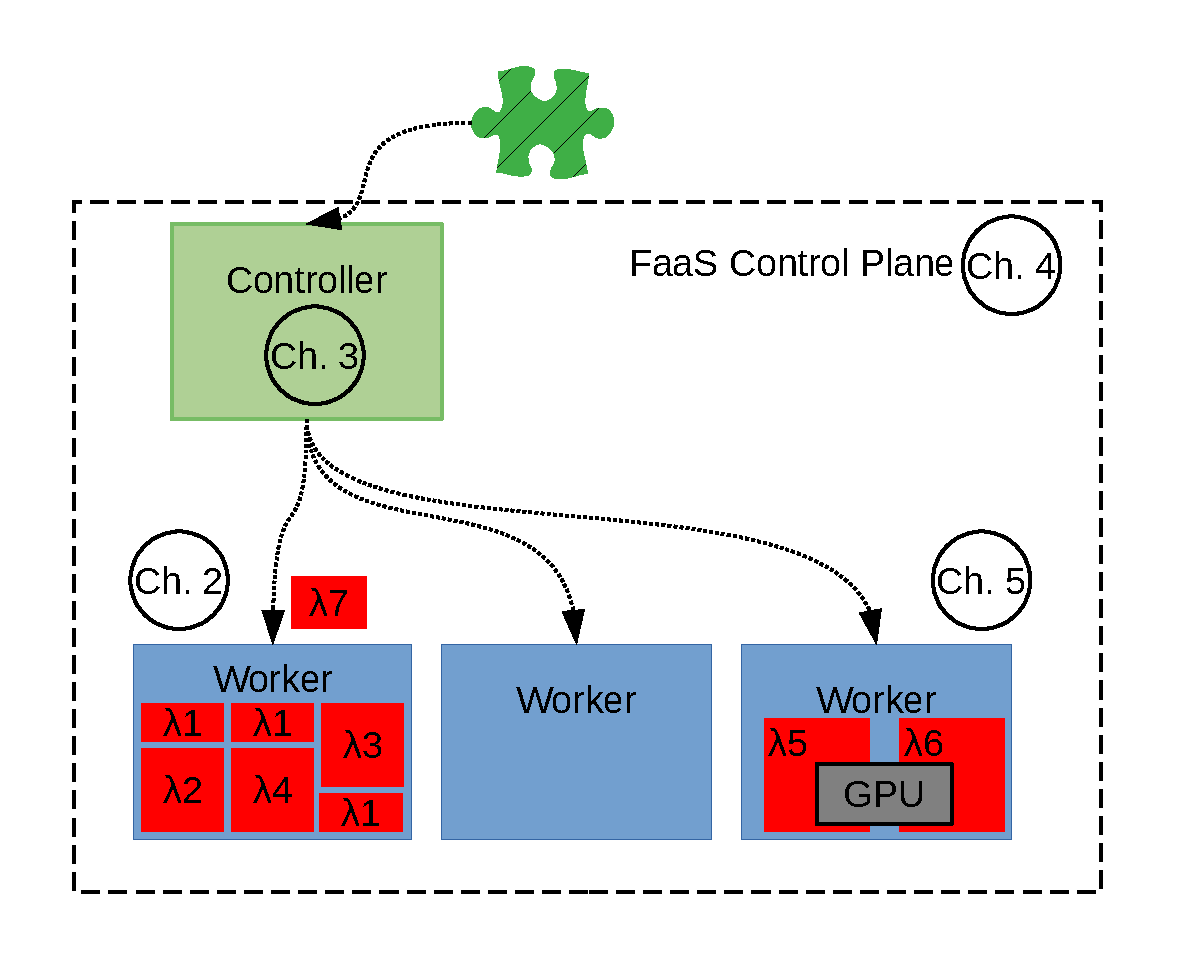
\includegraphics[width=\textwidth]{introduction/figs/faas-labeled.pdf}
  \caption{The major components of the control plane, and the areas of each this thesis impacts. A controller accepts invocations for functions and distributes them amongst a cluster of workers. These in turn run invocations in isolated sandboxes}
  \label{fig:control-plane}
\end{figure}

FaaS control planes themselves have been designed, re-design, and ported to a variety of ecosystems to solve unique problems and constraints.
% Nor is it a single "design" or platform
FaaS has been placed along the edge-to-cloud continuum~\cite{cicconetti2020decentralized,russo2023serverless,cheng2019fog,wang2020supporting}, taking advantage of its scale-to-zero capability.
% heterogeneous hardware
Moving serverless platforms beyond cloud computing to heterogeneous hardware has been explored~\cite{du2022serverless}, which is key for integration of IoT~\cite{persson2017kappa,trilles2020iot,cheng2019fog,wang2020supporting} and FPGA~\cite{bacis2020blastfunction,ringlein2021case} hardware.
% Private (Meta) 
Meta created an internal FaaS platform~\cite{sahraei2023xfaas} which could be optimized using their knowledge of what workloads run on it.
% FuncX
Another unique entry, FuncX~\cite{funcx_hpdc_20}, creates a layer over supercomputing resources to run user experiments in a FaaS-like manner.
% Cloud - GCP, Alibaba, AWS, Azure, several others
The most well-known platforms are the public offerings of the major cloud providers, AWS Lambda~\cite{lambda}, Google Functions~\cite{gcp-functions}, Azure Functions~\cite{azure-functions}, and Alibaba Function Compute~\cite{alibaba-compute}.
Several open-source equivalents have been made~\cite{openwhisk,openfaas,nuclio,knative} which are popular in both research and as products for end-users.
Included in this thesis is a design for a jitter-free, low-latency control plane and is highly configurable and able to run on heterogeneous and edge hardware.

% FaaS research isn't limited to a single domain
More focused research into serverless has branched into nearly every field of systems research.
To serve a function invocation, the system must create an isolated \emph{sandbox} to execute the user code in.
% A variety of isolation techniques predate FaaS~\cite{docker-main}, and were
Numerous isolation mechanisms have been put forward, containers~\cite{chhatrapati2021towards,docker-main,gvisor}, language runtimes~\cite{shillaker2020faasm,aytekin2019harnessing}, and lightweight virtualization~\cite{firecracker-nsdi20}.
All of these take time to start, in what's referred to as a \textit{cold starts} and can significantly increase invocation latency.
Additional research has targeted this problem specifically to accelerate existing isolation mechanisms creation time~\cite{mohan2019agile,du2020catalyzer,warm2}.
Future invocations see lower latency by benefiting from \emph{locality}, where the isolation sandbox is re-used in a \textit{warm start} invocation.

Knowingly keeping idle sandboxes resident in memory improves latency, but may lead to resource underutilization.
Sandboxes sizes are chosen by users, who often over-provision to negate performance problems~\cite{mvondo2021ofc,romero2021faa,eismann2021sizeless,yu2021harvesting,serverless-harvest-sosp21}.
Worker nodes also cannot host a container per function, who often require several for ideal performance, therefore remove them periodically to conserve space~\cite{faascache-asplos21}.
The highly heterogeneous workload of FaaS has proven challenging when trying to predict when containers will be needed, which would allow their removal from memory to conserve resources~\cite{shahrad2020serverless,zhao2021understanding}.
Adjusting the number of containers a function has reduces footprint, but may impact latency as they cannot be shared~\cite{enes2020real,li2022kneescale}.
Maintaining locality to provide acceptable performance while maximizing use of resources is an open area of research and addressed here.
% Keeping isolation containers around to serve future invocations requires their state to be maintained, typically in-memory.
% All possibly containers cannot be kept around because server resources are limited and valuable.
% The \textit{keep-alive} decision selects if and/or when containers are removed.

The serverless abstraction allows for workers with various capabilities, not limiting them to CPU-only computation.
The major cloud providers currently do not expose alternative compute, but latency-critical applications like machine learning (ML) inference being moved onto FaaS platforms to take advantage its high scalability can also benefit from heterogeneous hardware.
% Serverless functions currently cannot viably access CPU parallelism, and are configurable to use a limited number of CPU cores during execution. 
Accelerators come in many flavors: SmartNICs~\cite{choi2020lambda}, GPUs~\cite{pemberton2022kernel,guleria2019emf}, FPGAs~\cite{bacis2020blastfunction}, and more~\cite{du2022serverless,romero2021llama} -- each with unique characteristics and types of applications they can support.
A host of applications have moved to FaaS~\cite{yang2022infless,ali2022optimizing,zhang2019video,risco2021gpu,hung2019rapid,shankar2020serverless} that can leverage faster hardware.
FaaS invocations are also unable to easily coordinate computation with each other~\cite{yuan2022smpi,copik2023fmi,copik2022faaskeeper,sreekanti2020fault,sreekanti2020cloudburst,giantsidi2023flexlog,xu2021lambdadnn}, requiring slow intermediaries for interaction.
These accelerators also require locality to achieve usable performance, having significant and often longer cold start times.
% They also have a secondary effect
A unique \emph{data locality} for these devices exists too, as they must have data on hand that may have been cached on a system with more available memory.
Running accelerated and massively parallel computation in FaaS that puts not restrictions on applications is important for adoption and continued growth.

We cannot consider the challenges of serverless solely from a single-worker perspective, as by design it exists at a cluster level.
Functions have a variety of characteristics: execution time, inter-arrival-time of invocations, memory usage, and more.
These can all vary in orders of magnitude, from sub-second to several minute runtimes and sub-second to daily invocation arrivals~\cite{shahrad2020serverless}.
% The control plane is expected to guarantee low latency in all cases and scale applications up or down with changing demand.
Even worse, functions are notoriously bursty, rapidly changing how frequently invocations occur.
% In all, a FaaS control plane must handle millions of invocations per day and run them on clusters of thousands of machines.
% One could schedule function sandboxes, distinct from load balancing invocations~\cite{balaji2021fireplace,kaffes2021practical,abdi2023palette}, is a related problem to evenly distribute work across the cluster as functions vary with how many invocations they have.
One could schedule function sandboxes~\cite{balaji2021fireplace,kaffes2021practical,abdi2023palette,openwhisk} and have the controller micro-manage the cluster state.
% We must load balance~\cite{aumala2019beyond,leegreedy} invocations across clusters of servers and avoid overload any individual.
Load balancing invocations~\cite{aumala2019beyond,leegreedy,faaslb-hpdc22} is a more scalable way to address the complex load and large cluster uncertainty, trusting workers to make ideal decisions.
The cluster control plane targets locality in both cases, knowing that running invocations in existing sandboxes is much more performant.


% security~\cite{kim2023cryonics,zhao2023reusable,trach2019clemmys}
% applications~\cite{zhang2021serverless,mete2021implementation,hussain2019serverless,fouladi2019laptop,copik2022faaskeeper,hung2019rapid}
% % edge
% Edge serverless computing~\cite{aslanpour2021serverless,raith2023serverless,russo2023serverless}

% Domain-specific targets
% Low-latency~\cite{jia2021nightcore}
% Lang Runtime~\cite{shillaker2020faasm}
% FaaS as collection of services
% BaaS~\cite{baas,giantsidi2023flexlog,sreekanti2020cloudburst,sreekanti2020fault}


% Allows various trade-offs, in performance, security, and features.
% Serverless control planes have significantly different challenges and research opportunities than VM-based cloud computing.

\section{Thesis Outline}

% This thesis is consists of five additional chapters and is ordered as follows.
This thesis is ordered as follows.
The following chapter, Chapter~\ref{chap:serverless}, provides background on serverless computing, what technologies it builds on top of, and how it is being used in both research and by users.
Serverless evolved from, and is still built on top of, abstractions in cloud computing like virtual machines (VMs) and containers.
These mechanisms are used to isolate functions from one another and allow the control plane to control and protect resources.
This control plane itself consists of several components, a \emph{controller}, \emph{workers}, and ancillary services.
Users interact with the controller to create functions, invoke them, and receive results.
It, in turn, load balances invocations amongst the cluster of workers that execute them using the aforementioned isolation tools.
The many and varied designs presented by researches are shown and compared here.
Techniques to improve isolation mechanism performance and load balancing are frequent.
Wholly new systems have also been built, typically targeting a specific workload class such as ML, which has become popular in serverless.
This exploration ends with a detailing of the many use cases serverless has been put towards, including ML, scientific computing, and even distributed computing.

Chapter~\ref{chap:faascache} has the first contribution of this thesis and describes a container cache management design called \emph{FaasCache}.
%, and is about making smarter decisions in when to remove function containers.
Control planes keep idle function containers resident in memory in the expectation that they will be used again in the future.
These warm executions are significantly faster than their counterparts that must wait for a container to be spun up.
% In order to achieve low latency for individual function invocations, FaaS control planes must keep execution sandboxes resident in memory.
Unfortunately, memory is neither a free nor infinite resource, so control planes remove containers to both conserve and make room for others.
FaasCache optimizes worker memory usage by treating these containers as a \emph{cache}, and carefully considers what to evict when under resource constraint.
Each worker monitors function characteristics such as memory usage, frequency, and container startup time.
These are fed into a policy deciding which will be more valuable to keep given the cost of having to re-create it and how soon that might be.
It also monitors the cache-hit ratio of invocations to dynamically resize the memory allocated to the cache for targeting performance.
% This eviction decision is usually done on a timeout started when the last time a container was used.
% In this work I propose switching to on-demand resource reclamation and use several function and container attributes to decide what to remove.
% This algorithm applies ideas from the long-studied area of caching algorithms, who maximize utility out of fixed size resource pools.
% Container removal is analogous to cache eviction, and an invocation with or without an existing container can be considered a cache hit or miss.


The next chapter, chapter~\ref{chap:chrlu}, moves up a level in the control plane to present a novel load-balancing algorithm. % called 
As FaasCache shows, functions benefit from running in warm containers, which is referred to as function \emph{locality}.
The heterogeneous nature of functions would imbalance workers if we sent each function's invocations to a single worker.
Some would be overloaded and suffer significant performance degradation, others sitting idle.
Our \emph{CH-RLU} algorithm targets locality for functions while at the same time avoiding worker overload.
We use \emph{consistent hashing}~\cite{karger1997consistent} to give perfect locality and distribute functions amongst workers.
To detect overloads, we keep usage reports from each worker and add anticipated load from dispatched invocations to such reports.
Extremely popular functions, those with the highest frequency of invocations, also model Gaussian noise of the load impact before sending an invocation, to model overloading scenarios.
In all cases, if we predict a worker has too much work, we direct invocations away from it in a fixed pattern, maintaining locality while minimizing overloaded workers.
The effectiveness of this at both minimizing platform overhead and keeping load even across worker clusters is described at the end of the chapter.
% Serverless control planes do not operate on a single node, so load balancing algorithms are required to distribute invocations amongst workers.
% The load balancer must make a quick decision, and take into account the highly variable characteristics of functions it serves.
% A poor decision can drastically increase latency, as many functions execute in only a few milliseconds and scheduling delays can quickly exceed this.
% An algorithm must favor locality to achieve warm hits for functions, while ensuring workers are not overloaded from function frequency imbalance.
% To find this balance I propose a mixture of a function pinning load-balancing algorithm that is informed by existing load status to avoid overcommitment.
% This will minimize latency from CPU timesharing and favor warm invocation executions.

Next, Chapter~\ref{chap:iluvatar} details a new serverless control plane design called \sysname.
% created to fix problems with existing open-source offerings.
% Current open-source FaaS control planes \cite{openwhisk} are deficient in key areas for promoting scalable research in the area.
This new control plane is written in Rust and seeks to solve the deficiencies in current open-source control planes used for research~\cite{openwhisk}.
Its worker is designed to be highly modular, allowing swap-able implementations to support heterogeneous platforms and ease comparisons for research.
It supports a novel queue mechanism to support new designs that may not run all workloads immediately, or handle cases of severe resource demand.
The controller is built on a stateless design and uses the load balancing algorithm from Chapter~\ref{chap:chrlu}, relying on the worker's local knowledge for scheduling.
The third runtime component is a time-series database~\cite{influx} used to aggregate function and worker metrics, reducing communication overhead between platform components.
Finally, and a first for such systems, it has a built-in load generation suite that integrates seamlessly with both worker and load balancer.
With this, one tool can test any level of the control plane under various load conditions, and record highly detailed information for post-experimental analysis.
We use this tool to compare with other control plans and show the performance benefits of \sysname.
% They can have a variety of issues, such as significant performance spikes, a brittle code structure for modification, lock-in to various technologies, and poor setup for consistent experimentation.
% I detail a new serverless control plane that will be designed with two goals in mind: be effective for enabling research and low variability latency.
% Having a low and controlled latency is critical for having confidence in experimental results, the ability to attribute data to changes you made.
% The control plane being easily extensible and integrating seamlessly with a load generation framework is vital to productive research.

% Chapter~\ref{chap:new-poly} polymorphic functions are proposed as extensions to serverless capabilities.
% Chapter~\ref{chap:new-mpi} serverless MPI is proposed as extensions to serverless capabilities.
The final piece of this thesis is Chapter~\ref{chap:gpu-sched}, which uses \sysname~to multiplex GPU resources to serve black-box functions.
To prevent maintain control of GPU resources, we insert a \emph{shim} in between the function and GPU driver to intercept calls.
This lets us both over-subscribe memory and control when the memory is on-device or moved to the host.
We leverage the increase in memory control to allow many containers to share one GPU, creating a \emph{warm-pool} similar to that of regular CPU serverless.
As GPUs cannot support the same concurrency as many-cored CPUs, we use the queue mechanism of \sysname~to dynamically control ordering and dispatching of invocations.
The queue monitors GPU utilization and sends invocation when compute is available, moving memory around to ensure we don't overload the device.
Invocations also benefit from locality here, successive runs and having their memory available gives better execution performance.
We balance these needs with fairness, using the queue to prevent any function from starving others of device time.
The effectiveness of all these are demonstrated with thorough experimental analysis at the end of this chapter.
% Users want to run workloads, especially ML inference jobs, with low latency and this requires using accelerators.
% Modern serverless systems only expose CPU compute capabilities, while some bespoke research systems target inference-only workloads.

% Chapter~\ref{chap:summary} concludes this thesis.


\chapter{Background: Serverless computing and Function as a Service}
\label{chap:serverless}

% more opening context needed
% why should someone read this chapter?
Serverless computing builds on architectures and designs used throughout cloud computing.
These have been adapted and specialized in a myriad of ways by researchers and companies to both improve performance and enable new features.
This chapter starts by describing in detail how serverless cloud control planes operate, and the systems used to build them.
Additionally, the plethora of FaaS research in areas related to this thesis are examined and compared against.

\section{What exactly is Serverless Computing?}
\label{sec:serverless-computing}

\begin{figure}
  \begin{center}
    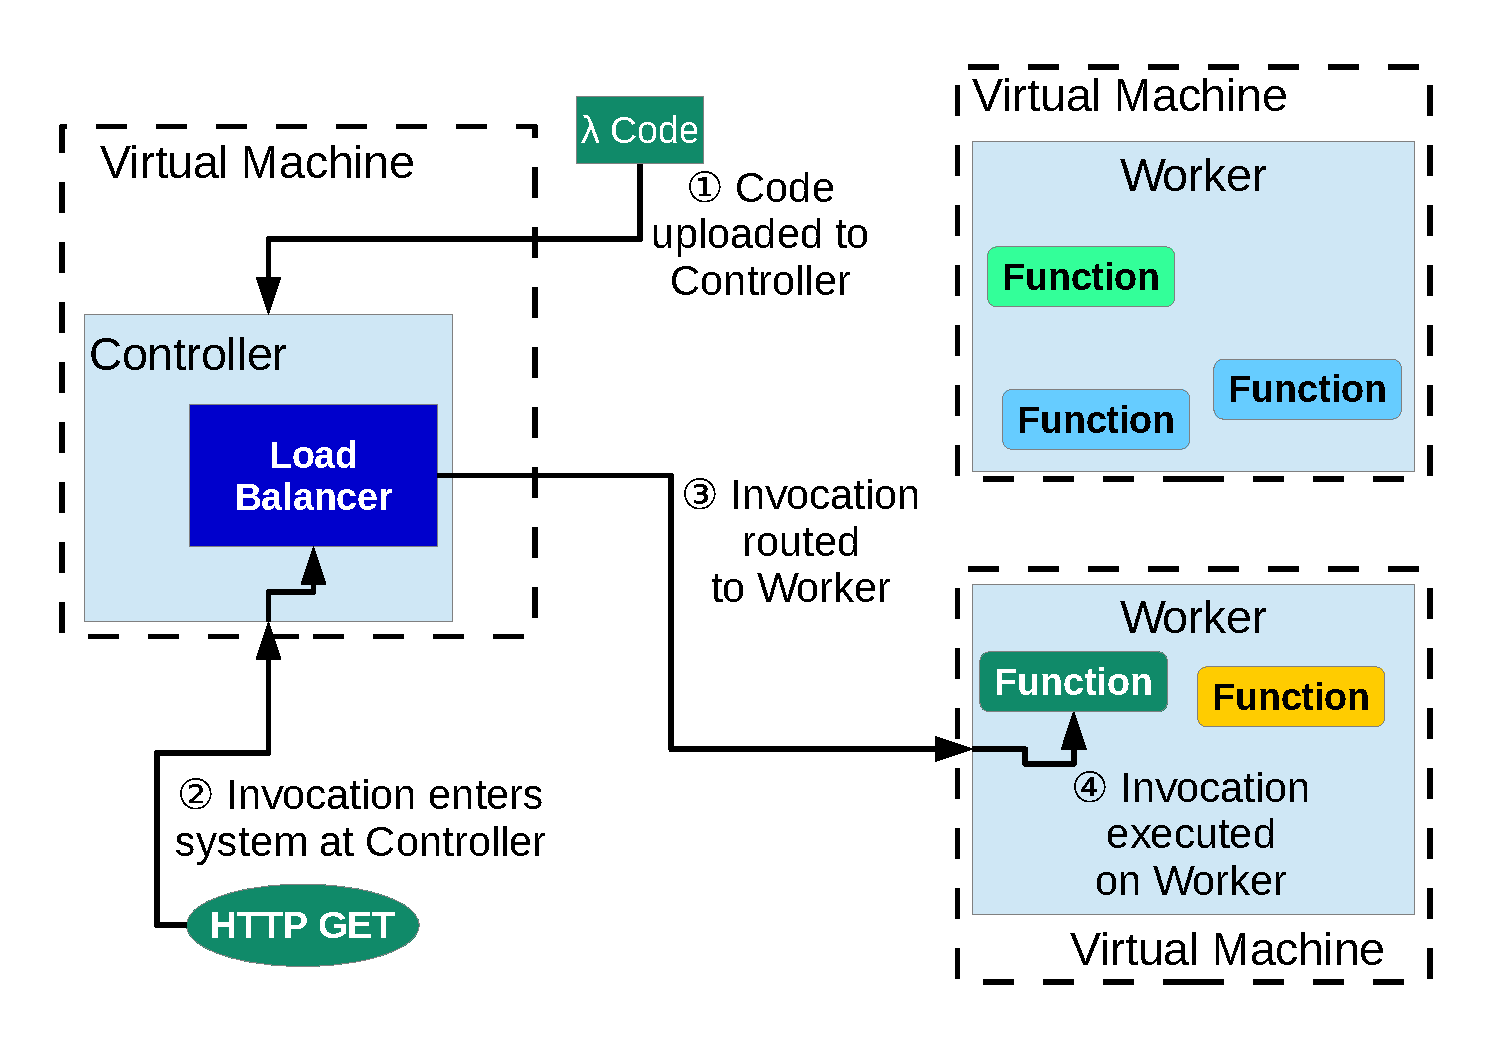
\includegraphics[width=.9\columnwidth]{./figures/sys-diag.pdf}
  \caption{A common architecture for serverless control planes. 
          A controller distributes invocations to workers who run them inside containers.}
  \label{fig:serverless-arch}
\end{center}
\end{figure}

% Continuing the container abstraction to its most extreme conclusion, we get a leap to \textit{serverless computing} often called Function-as-a-Service (FaaS).
Serverless computing presents a radical departure from previous iterations of computing architectures.
Users can run arbitrary applications without concern for how or where it is ultimately run.
FaaS control planes operate as a complex distributed system, operating from the lowest levels of OS abstractions to the highest levels of cloud system designs.

All such control planes work similarly and follow the generic architecture shown in Figure~\ref{fig:serverless-arch}.
Users upload their \textit{source code} \circled{1} such as that one in Figure~\ref{fig:background-lambda-example} to the cloud provider to create a \textbf{function}, and such functions can be chained together inside the provider's system to form a larger \textbf{application}.
When the code is \textbf{invoked} (e.g. an HTTP request is made \circled{2}), the provider routes it to a worker \circled{3}, creates a sandbox for it and executes the function \circled{4}, passing in any custom parameters.
This sandbox must provide isolation, both covering both resource and security, ensuring that hogs or malicious actors do not interfere with co-located executions.
Often, this sandbox utilizes existing technologies such as Docker \cite{docker-main} or VMs.
The major cloud computing providers have all created offerings, Amazon Lambda \cite{lambda}, Google Cloud Functions \cite{gcp-functions}, Azure Functions \cite{azure-functions}, alternative providers such as IBM \cite{openwhisk} and Alibaba \cite{alibaba-compute} have joined in, and even non-commercial open-sourced control planes exist \cite{hendrickson2016serverless,openfaas}.

\begin{figure}
  \begin{lstlisting}[language=Python, numbers=left, frame=single, basicstyle=\footnotesize\sffamily, columns=fullflexible]
  # Initialization code 
  import numpy as np 
  import tensorflow as tf
    
  m = download_model('http://model_serve/img_classify.pb')
  session = create_tensorflow_graph(m) 
    
  def lambda_handler(event, context):
       # This is called on every function invocation 
       picture = event['data']
       prediction_output = run_inference_on_image(picture) 
       return prediction_output 
     \end{lstlisting}
     \caption{A classic serverless function: performing ML inference on image data. 
              In this example library and model initialization are done before execution starts.}
     \label{fig:background-lambda-example}
\end{figure}

\begin{comment}
  \begin{figure}
  \begin{lstlisting}[frame=single, basicstyle=\footnotesize\sffamily, columns=fullflexible]
GET http://faas.com/img_recogn?input_bucket=9bcc64b9.png
  \end{lstlisting}
  \caption{Invoking a serverless function to perform image recognition. Small inputs may be passed directly, with large ones passed indirectly via storage.}
  \label{fig:lambda-invoke}
\end{figure}
\end{comment}

In a change from the billing model for rented VMs, users are billed only for the time their code is executing, often in small millisecond-sized time slices.
Most providers set the cost to a formulation of the amount of memory used per time period \cite{lambda-pricing}, roughly $\$1.66 \times 10^{-5}$ per GB/second.
Should the provider choose to keep that sandbox resident in memory to use for a future invocation, the user will not be charged nor be aware that it is happening, save for lower latency on future invocations.

% \cite{lambda,gcp-functions,azure-functions,openwhisk,alibaba-compute,shahrad2020serverless,hendrickson2016serverless}


Serverless computing is now being provided by all large public cloud providers and is an increasingly popular way to deploy applications on the cloud.  
%Amazon Lambda~\cite{aws-lambda}, Google Functions~\cite{google-functions}, and Azure Functions~\cite{azure-functions} are becoming an
Functions as a Service (FaaS) can also be realized on private clouds and dedicated clusters using frameworks such as OpenWhisk~\cite{openwhisk}, OpenFaaS~\cite{openfaas},  OpenLambda~\cite{hendrickson2016serverless}, etc. 
In this new cloud paradigm, users provide functions in languages such as Python, JavaScript, Go, Java, and others. 
The functions are executed by the FaaS platform, greatly simplifying resource management for the application. 



% Need to explain how it all works. But first provide some context for why this is important.


%In order to provide FaaS, the way it is implemented by platforms, results in certain performance challenges.
%However, the execution of FaaS functions entails performance overheads that we must be cognizant of. 
%
%FaaS functions cannot assume that state will persist across invocations, and functions need to be self contained in terms of their dependencies. 
%
FaaS functions cannot assume that state will persist across invocations, and function definitions must first import and load all code and data dependencies on each execution. 
Each function is run inside a container such as Docker~\cite{docker-main}, or a lightweight VM such as Firecracker~\cite{firecracker-nsdi20}. 
By encapsulating function state and any side effects, the virtual execution environment provides isolation among multiple functions, and also allows for concurrent invocations of the same function. 
Due to the overhead of starting a new virtual execution environment (i.e., container or VM), and initializing the function by importing libraries and other data dependencies, function execution thus incurs a significant \quotes{cold-start} penalty.
Table~\ref{tab:bg-workloads} shows the breakdown of initialization time (last column) vs. the total running time of different FaaS applications, and we can see that the initialization overhead can be as much as 80\% of the total running time. 
Thus, FaaS can result in significant performance (i.e., total function execution latency) overheads compared to conventional models of execution where applications can maintain application state between handling user requests and do not face the high initialization and cold-start overheads. 



\begin{table}
  \centering
  \caption{FaaS workloads are highly diverse in their resource requirements and running times. The initialization time can be significant and is the cause of the cold-start overheads, and depends on the size of code and data dependencies.}
  \begin{tabular}{lrrr}
    \hline 
    Application & Memory size & Run time & Initialization time \\
    \hline
    ML Inference (CNN) & 512 MB & 6.5 s & 4.5 s \\
    Video Encoding & 500 MB & 56 s & 3 s \\
    Matrix Multiply & 256 MB & 2.5 s & 2.2 s \\
    Disk-bench (\texttt{dd})  & 256 MB & 2.2 s & 1.8 s \\
    % Image Manip & 300 MB & 9 s & 6 s \\
    Web-serving & 64 MB & 2.4 s & 2 s \\
    Floating Point & 128 MB & 2 s & 1.7 s \\

    \hline
  \end{tabular}
  % \vspace*{\myfigspace}
  \label{tab:bg-workloads}
  %\vspace*{\myfigspace}
\end{table}



% Replace two main techniques -> Only one technique. 
%Two main techniques are used to alleviate the cold-start penalty. 
Once a container for a function is created and the function finishes execution, the container can be kept alive instead of immediately terminating it. 
Subsequent invocations of the function can then \emph{reuse} the already running container.
This \emph{keep-alive} mechanism can alleviate the cold-start overhead due to container launching (which can be $\sim 100$ ms). %Might be confusing, keep-alive also helps in other initialization.



However, keep-alive is not a panacea for all FaaS latency problems. 
Keeping a container alive consumes valuable computing resources on the servers. %, and reduces the number of functions that can be executed concurrently. 
Specifically, a running container occupies memory, and \quotes{warm} containers being kept alive in anticipation of future function invocations can reduce the multiplexing and efficiency of the servers. 
Thus, we develop keep-alive \emph{policies} that reduce the cold-start overhead while keeping the server utilization high.
%

Designing general keep-alive policies is challenging due to the extreme heterogeneity in the different function popularities, resource requirements, and cold-start overheads.
For instance, a recent analysis of FaaS workloads from Azure~\cite{shahrad_serverless_2020} shows that function inter-arrival times and memory sizes can vary by more than three orders of magnitude. 
%
This workload heterogeneity magnifies the performance vs. utilization trade off faced by keep-alive policies, as we shall describe in the next section. 
Additionally, FaaS workloads also show a high temporal dynamism, which requires new approaches to resource provisioning and elastic scaling, which we also develop. 

\section{Serverless Containers}
\label{sec:virtualization}


\subsection{Virtual Machines}

% Turtles all the way down.
% The public cloud is build on virtualized components.
% Compute providers have vast quantities of physical hardware and sell virtualized resources to customers \cite{amazon-ec2, azure-compute, google-compute}.
% Rather than having to procure and 

To both prevent takeover of the physical hardware and ensure isolation between different users, cloud providers typically offer virtualized infrastructure \cite{xen}.
Mimicking the stack in Figure~\ref{fig:vms}, user applications run inside a virtual machine and cannot directly access the hardware.
A hypervisor manages a series of virtual machines that have a private OS inside them.
Using hardware virtualization techniques, the provider's hypervisor interposes itself between guest and hardware, maintaining total control.
Memory is protected via virtual memory in the CPU, protected instructions are trapped to the hypervisor, and network and disk I/O interaction can be run through the hypervisor.
A major drawback is that users must install (duplicate) copies of OS's, libraries, and applications into each VM, and are responsible for maintenance of the guest OS.

% Basic outline of a Virtualization setup.
% Hypervisor, Mangagement software, various guests.
% hypervisor imposes as fake version of hardware for isolation.

\subsection{VM Resource Management}

% Boil 'em, mash 'em, stick 'em in a rack.
% Oodles of work in the maximizing resource use in area.
% From making them faster, reducing footprint, bin-packing, etc.
A number of works have sought to reduce the overhead from virtualization by techniques such as securely exposing hardware to guests \cite{dong2008sr} or reducing layers of indirection \cite{ben2010turtles}.
A number of optimizations to memory usage that reduce the footprint of VMs were outlined by~\cite{waldspurger2002memory}, which are still used in production hypervisors today.
Choosing where to place VMs, knowing that they may run for days or months, is critical to reduce fragmentation on hosts across provider datacenters.
Bin-packing studies have sought to minimize fragmentation \cite{binpacking} by overcommitting resources even at the risk of violating capacity.
Even today, after much research in the area, providers see 20\%-40\% of unallocated resources~\cite{fuerst2022memory} that they seek ways to make use of.

\subsection{Containers}

% \begin{figure}
%   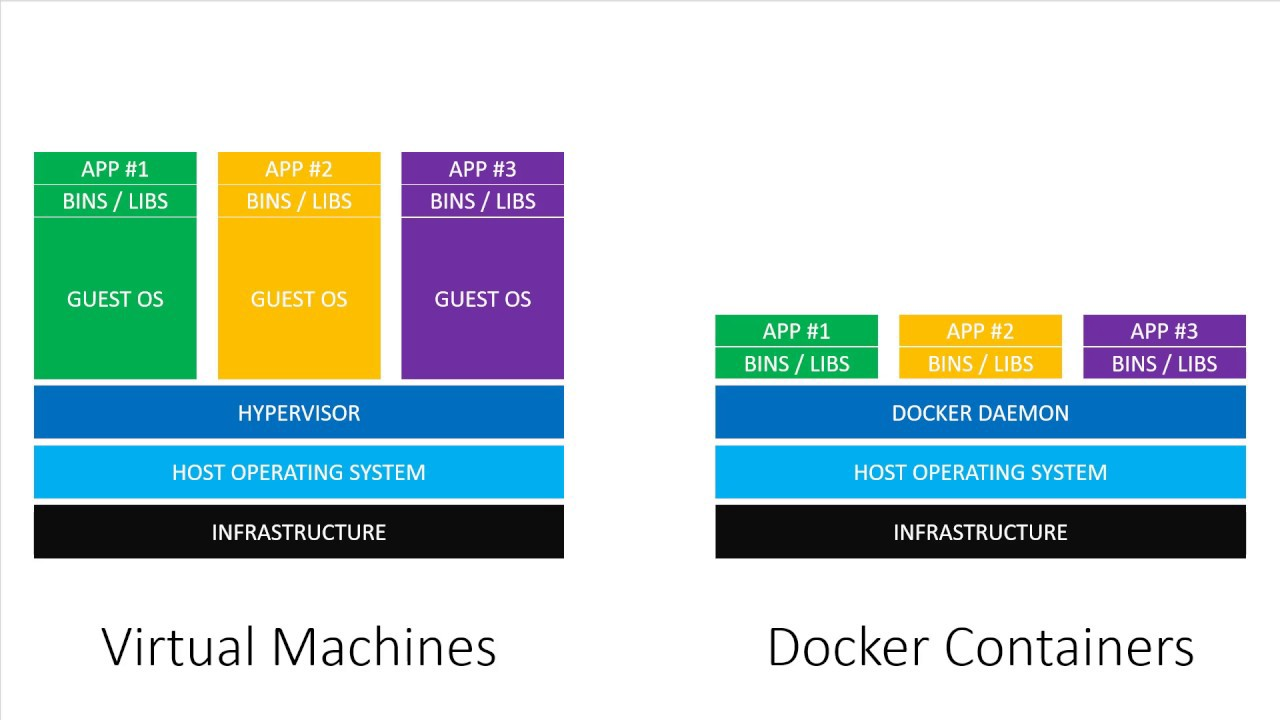
\includegraphics[width=\columnwidth]{figures/docker-vs-vms.png}
% \end{figure}

\begin{figure}
  \subfloat[Virtual Machines]{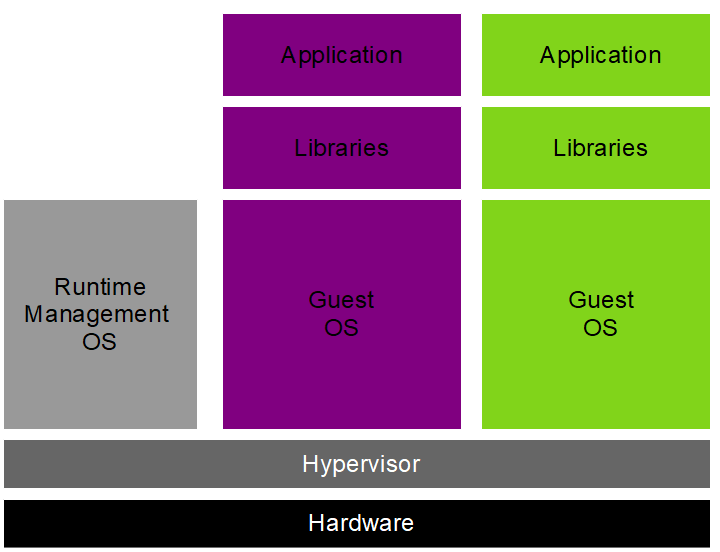
\includegraphics[width=0.5\textwidth]{serverless/figs/vms.png} \label{fig:vms}}
  \subfloat[Containers]{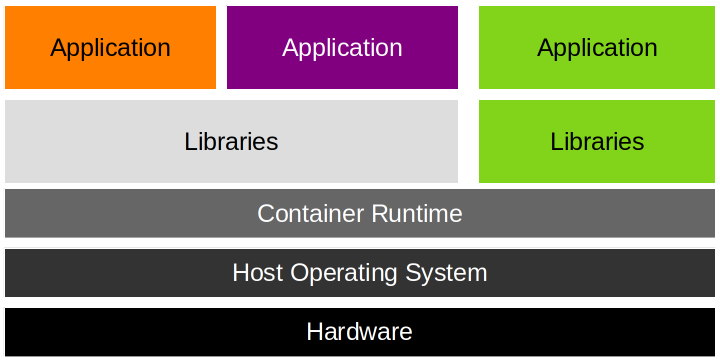
\includegraphics[width=0.5\textwidth]{serverless/figs/containers.png} \label{fig:docker}}
  \caption{Different layers of abstraction between hardware and kernel based virtualization.}
  \label{fig:docker-vs-vms}
\end{figure}

Enabling both improved process-level protections and a viable alternative to hardware virtualization, a new method of isolation was devised.
Kernel virtualization, built originally around Linux \textit{cgroups}, provides similar isolation and security guarantees to VMs.
A combination of kernel utilities enables limiting CPU, memory, and I/O usages, restricting views of the file system, blocking interaction with other processes, and more.
Popularized by various projects \cite{oci,docker-main}, such \textit{containers} reimagined how cloud computing and applications could work.
Multiple applications could share the same operating system, and even libraries, safe from all interference from one another.
Developers could ship applications, complete with any dependencies, that ran securely, anytime, and anywhere.
Providers even began offering services around these, tools like Kubernetes \cite{kubernetes} orchestrate placement of containers onto hosts, removing the need for users to rent VMs at all.


\section{Serverless Control Plane Research}
\label{sec:platform-enhance}

\mhead{Cold Start Mitigation}
The FaaS computing paradigm sees providers running user code on-demand when a request comes in, and importantly deciding \emph{where} it should run. 
Each invocation must be run in isolation from co-located invocations and must ensure provider control over system resources.
Both security goals are thus achieved by running each invocation in a sandboxed environment. 
Sandboxes are generally implemented using containers (such as Docker~\cite{docker-main}) or lightweight VMs (such as Firecracker~\cite{firecracker-nsdi20}) created on the server that runs the invocation.
Unfortunately, creation time for both any type of sandbox can be significant, adding latency to the in-flight request. 

Many techniques have been proposed to reduce the initialization overhead from such \emph{cold starts}.
Cold start invocations, because of the large initialization overheads, are typically $1-10\times$ larger than the function execution time.
%  which occurs when the function is run in an already initialized container which is cached in memory. 
% They can be mitigated by skipping initialization entirely, by saving in memory and reusing the execution environment for subsequent invocations of the same function. 
We can mitigate this by the saving execution environment in memory and reusing it for subsequent invocations of the same function, skipping initialization entirely. 
Keeping the function \quotes{warm} thus allows a provider to amortize the startup cost across future invocations.

\mhead{Workload Characterization}
Published traces from major providers give a glimpse into the scale of serverless computing.
Shahrad et al.~\cite{shahrad_serverless_2020} publicized the first dataset of the functions served by Azure Fucntions, with a detailed characterization breakdown.
As seen in Figure~\ref{fig:wild-invokes}, invocation rates are \emph{extremely} heavy tailed.
% 0.1\% of functions account for half of all invocations, and the top 19\% account for a total of 99.6\% of invocations.
The most frequently invoked functions are executed several times a second, while the rarest perhaps once per day.
Because of this, a small portion, 19\% of functions, account for 99.6\% of invocations in Azure.
A paper describing an internal FaaS platform at Meta~\cite{sahraei2023xfaas}, showcased handling trillions of invocations daily and a similar skewed workload.

Several examples of functions are shown in Table~\ref*{tab:workloads}, these are taken from~\cite{functionbench}.
Functions have high variation in warm and cold-start times, with cold-start times being significantly higher.
Memory usage can range from a few dozen megabytes, to half a gigabyte, matching real-world data from~\cite{shahrad_serverless_2020}.
Control planes must be able to handle these high variations in frequency and resource usage, and treat all functions fairly.

\begin{figure}
  \begin{center}
    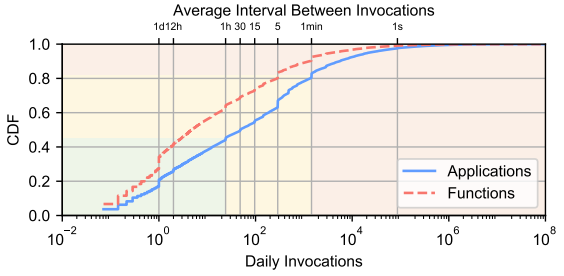
\includegraphics[width=.9\columnwidth]{./figures/wild-invocations.png}
    \caption{A CDF of daily invocations for functions. 
              Invocation frequencies range from sub-second to less than one per day. 
              Figure from~\cite{shahrad_serverless_2020}}
  \label{fig:wild-invokes}
\end{center}
\end{figure}

Functions exist in a data-driven architecture, being required to download inputs to handle each invocation.
The same group at Azure released another dataset in~\cite{romero2021faa}, focusing on data usage of functions.
They found a split of functions with some having high cloud storage usage and others almost none.
Surveys have shown that applications of all types have been deployed on FaaS~\cite{raza2021sok,hossein2022survey,eismann2020serverless}.
Some examples are explored in Section~\ref{sec:serverless-apps}.
% Control planes must cater to a host of diverse applications with equally varied runtime needs.

% The warm and cold time for different functions from the FunctionBench~\cite{kim_functionbench_2019} workload suite are shown in Table~\ref{tab:func-times}.
% The table shows the total execution latency when these functions are run on OpenWhisk.

\begin{table}
  \centering
  \caption{FaaS workloads are highly diverse in their resource requirements and execution times. The initialization time can be significant and is the cause of the cold-start overheads, and depends on the size of code and data dependencies.}
  \begin{tabular}{lrrr}
    \hline 
    Application & Mem size & Warm time (sec) & Cold-start time (sec) \\
    \hline
    % Web-serving & 64 MB & 2.4 s & 2 s \\
    % ML Inference (CNN) & 512 MB & 6.5 s & 4.5 s \\
    % Disk-bench (\texttt{dd})  & 256 MB & 2.2 s & 1.8 s \\
    % Floating Point & 128 MB & 2 s & 1.7 s \\
    % Image Manipulation & 300 MB & 9 s & 6 s \\
    % Matrix Multiply & 256 MB & 2.5 s & 2.2 s \\
    % Video Encoding & 500 MB & 56 s & 3 s \\
    Web-serving & 64 MB & 0.179 & 1.153 \\  
    ML Inference (CNN) & 512 MB & 2.211 & 7.833 \\
    Disk-bench (dd) & 256 MB & 1.068 & 2.944 \\  
    Floating Point & 128 MB & 0.083 & 1.432 \\  
    Image Manipulation & 300 MB & 4.806 & 5.268 \\  
    Matrix Multiply & 256 MB & 0.117 & 1.067 \\  
    AES Encryption & 128 MB & 0.587 & 2.064 \\  
    Video Encoding & 500 MB & 10.28 & 11.51 \\  
    JSON Parsing & 256 MB & 0.414 & 1.962 \\
    \hline
  \end{tabular}
  \label{tab:workloads}
\end{table}


\begin{comment}
\begin{table}
  \begin{tabular}{ c c c }
\hline
  Application & Warm Time (s) & Cold Time (s) \\ 
\hline
  Web-serving & 0.179 & 1.153 \\  
  ML Inference (CNN) & 2.211 & 7.833 \\
  Disk-bench (dd) & 1.068 & 2.944 \\  
  % float & 0.083 & 1.432 \\  
  % gzip & 0.406 & 1.033 \\  
  % image & 4.806 & 5.268 \\  
  Matrix Multiply & 0.117 & 1.067 \\  
  Sklearn Regression & 53.57 & 54.45 \\  
  AES Encryption & 0.587 & 2.064 \\  
  Video Encoding & 10.28 & 11.51 \\  
  JSON Parsing & 0.414 & 1.962 \\
\hline
\end{tabular}
\caption{FunctionBench~\cite{kim_functionbench_2019} functions run times' are significantly longer on cold starts. Ideally we want all of our functions to run warm to lower user latency. Cold starts also increase system load by creating runtime overhead.}
\label{tab:func-times}
%\vspace*{-0.4cm}
\end{table}
\end{comment}

\mhead{Reusing Initialization}
Performing multiple container startups of a function will involve executing the same startup procedures repeatedly: language runtimes, the OS of a micro-VM, etc.
Utilizing past startups by checkpointing the container at a known position and booting from there has proved promising in reducing cold start times~\cite{du2020catalyzer,vhive-asplos21}.
Memoization approaches that leverage existing containers to duplicate their state have proven highly effective~\cite{du2020catalyzer,wei2022booting}.

\mhead{Alternate Isolation Mechanisms}
While a simple implementation would run functions inside Docker containers~\cite{docker-main}, so long as isolation guarantees are upheld, using alternate mechanisms with faster start times is effective.
Directly optimizing the isolation mechanism~\cite{firecracker-nsdi20} or common libraries and language runtimes used by FaaS worklaods~\cite{carreira2021warm} both give immediate performance boosts. 
Running functions inside the worker's language runtime can dramatically reduce initialization times~\cite{vhive-asplos21,shillaker2020faasm,jia2021nightcore,du2020catalyzer}.
Security may be relaxed between functions in a larger application~\cite{akkus_sand_2018, dukic2020photons} allowing for the reuse of sandboxes.
%

\mhead{FaaS Resource Management}
Worker resources are not infinite, especially memory for keeping function sandboxes available.
Packing functions together can improve memory utilization~\cite{akhtar_cose_2020}.
Developers often over-assign memory, causing under-utilization, the control plane is in the perfect place to minimize this waste~\cite{eismann2021sizeless, mvondo2021ofc}.
Concurrent invocations of the same function has been reused to share resources, as isolation may be relaxed~\cite{stojkovic2023mxfaas}.

The initialization overheads of serverless functions and their repeated invocations have spawned a great deal of research into optimizing their resource management.
Recent surveys~\cite{faas-survey-jan-2022, raza2021sok, eismann2020serverless, hassan2021survey, mampage2021holistic} provide an overview of the challenges and solutions in this very active research area. 

% Locality for FaaS resource management has been explored in the form of function keep-alive policies~\cite{shahrad_serverless_2020}. 
% Once a container for a function is created and the function finishes execution, the container can be kept alive instead of immediately terminating it. 
% Subsequent invocations of the function can then \emph{reuse} the already running container.
% This \emph{keep-alive} mechanism can alleviate the cold-start overhead due to container launching (which can be $\sim 100$ ms). %Might be confusing, keep-alive also helps in other initialization.

% However, keep-alive is not a panacea for all FaaS latency problems. 
% Keeping a container alive consumes valuable computing resources on the servers. %, and reduces the number of functions that can be executed concurrently. 
% Specifically, a running container occupies memory, and ``warm'' containers being kept alive in anticipation of future function invocations can reduce the multiplexing and efficiency of the servers. 
% Thus, we develop keep-alive \emph{policies} that reduce the cold-start overhead while keeping the server utilization high.

% Designing general keep-alive policies is challenging due to the extreme heterogeneity in the different function popularities, resource requirements, and cold-start overheads.
% For instance, a recent analysis of FaaS workloads from Azure~\cite{shahrad_serverless_2020} shows that function inter-arrival times and memory sizes can vary by more than three orders of magnitude. 
% This workload heterogeneity magnifies the performance vs. utilization tradeoff faced by keep-alive policies, as we shall describe in the next section. 
% Additionally, FaaS workloads also show a high temporal dynamism, which requires new approaches to resource provisioning and elastic scaling, which we also develop. 

% Single-server environments have been the focus of these mechanisms and policies: we have made an initial attempt to understand their interactions in a distributed cluster context.
% Inter-function dependencies can also be used for predictive resource management and reducing function communication and startup costs~\cite{gunasekaran2020fifer, daw2021speedo, shen2021defuse}: incorporating these policies into our load-balancer is part of future work. 

\subsection{Load Balancing}

Serverless control planes are a distributed system, assigning invocations to worker nodes.
The load-balancing of invocations can significantly affect latency, from either overloading workers or causing excessive cold starts. 
Several works have used locality as the primary way of ensuring invocation warm-starts, trying to direct a function to the same worker(s)~\cite{package-cristina-19, leegreedy}.
FaaS load-balancing may be seen as akin to VM bin-packing, and some have used reinforcement learning to choose sandbox placement~\cite{balaji2021fireplace}.
Predicting a window of function's invocation arrivals and preparing a container for it~\cite{shahrad2020serverless} works for relatively uncommon functions.
Scheduling functions based on their larger application DAG can minimize startup and communication time~\cite{shen2021defuse, abdi2023palette, guo_decomposing_2022, kotni2021faastlane, shen_defuse_2021,mahgoub_wisefuse_2022,zhou_qos-aware_2022}.
Functions may compete for certain resources like network, so scheduling them on different machines can speed up certain workloads~\cite{tian_owl_2022}.

Package-aware load balancing~\cite{package-cristina-19}  identifies and uses function code dependencies (software packages) as an important source of data locality.
While this is an important factor, we focus on the in-memory locality of kept-alive functions since memory capacity is much smaller than permanent storage and caching functions in memory has a very large performance impact.
%
CPU contention and interference is a major source of performance bottlenecks for co-located functions, and adjusting CPU-shares using cgroups can provide significant benefits~\cite{suresh2019fnsched, suresh2021servermore, ensure-faas-acsos20}.
%
The load-locality trade off we explore is complementary to these CPU scheduling optimizations. 
%
The repetitive nature of functions and their workflows can also be used to improve resource utilization and latency~\cite{hunhoff2020proactive, yu2021faasrank, puru_xanadu_20, przybylski2021data}: our load-balancer is stateless for the sake of simplicity and can be enhanced with these techniques if necessary.


The tradeoff between locality and performance has also been explored in the context of delay scheduling~\cite{zaharia2010delay} for data-parallel applications such as MapReduce.
Load-balancing is seen as a \quotes{dispatch} problem in queuing theory, and the FaaS cluster system most closely approximates G/G/PS, since the arrivals and service times are not Markovian.
Techniques such as \quotes{join the shortest queue}, and \quotes{least work left}~\cite{gupta2007analysis} have been shown to be effective.
The online-greedy policy evaluated in the previous section closely approximates least-work-left.
However, it is difficult to implement in practice since the running times of functions is hard to predict due to their volatile arrival distribution mixtures and high variances in running time due to various system interference effects.


\subsection{Heterogeneous Hardware}

Numerous control plane designs have been proposed targeting various accelerators such as SmartNICs, GPUs, DPUs, and FPGAs~\cite{choi2020lambda,du2022serverless,pemberton2022kernel,daw2021speedo}.
One load balancing design sought to lower latency by mixing in low- and high-end servers for executing functions~\cite{roy2022icebreaker}, using cheap and plentiful memory to host many sandboxes with a few fast machines to speed up popular functions.

\subsection{Serverless Data-plane}

A lot of work has gone into improving the performance hit caused by serverless functions needing to repeatedly download data and state from remote storage.
Commonly used data can be cached on worker nodes for faster function access~\cite{mvondo2021ofc,romero2021faa}.
Fault-tolerant storage systems targeting serverless systems can accelerate shared worker between invocations~\cite{giantsidi2023flexlog,sreekanti2020fault}.
Co-locating different functions that access the same data to identical machines can improve data locality~\cite{abdi2023palette}.

\begin{comment}
\section{Application Orchestration}
\label{sec:app-orch}

Serverless providers only support single input-output and simple DAG organization of function invocations.
Several works have made orchestrators than run outside the provider serverless system to coordinate work.
\cite{suresh2021servermore, jonas2017occupy, fouladi2019laptop}
\end{comment}

\section{Application Mitigations of Control Plane Deficiencies}

Researchers have often found the offerings by cloud providers to be lacking, but naturally do not want to host their own serverless control plane.
To compensate for this, many have developed workarounds for issues such as poor performance and missing features.
Even cloud providers face bottlenecks when rapidly scaling a function to several thousand workers, hence~\cite{basu2023propack} allocates very large sandboxes and manually run multiple functions inside them.
To overcome the lack of communication,~\cite{copik2023fmi} creates a secondary VM to punch TCP/IP holes that enables an MPI-like interface for custom Python functions.
% Work done to get around the lack of features in current providers, or performance characteristics therein.


\section{Serverless Applications}
\label{sec:serverless-apps}

A variety of applications have been built on serverless computing, in all manner of industries, use cases, and scales.

FaaS can be used to distribute embarrassingly parallel tasks such as MapReduce~\cite{jonas2017occupy} or a \texttt{make} task~\cite{fouladi2019laptop}.
A common use case is parallel encoding of videos using hundreds of workers~\cite{ao2018sprocket, zhang2019video} or performing analytics on live video~\cite{romero2021llama, risco2021gpu}.
On-demand scaling and usage has made FaaS attractive as a place to run streaming applications~\cite{konstantoudakis2022serverless,wang2021wearmask,elordi2021demand} and real time~\cite{yan2016building,anand2019low} tasks.

The event-driven nature of serverless execution has garnered a lot of excitement from the IoT community~\cite{benedetti2021experimental,trilles2020iot,hu2020hivemind,persson2017kappa}.
Edge computing pairs nicely with the ephemeral and on-demand execution model of serverless and has seen significant work~\cite{cicconetti2020decentralized,cheng2019fog,wang2020supporting}.
Industrial applications, especially for monitoring and control have proven popular~\cite{hussain2019serverless,mete2021implementation,zhang2021serverless}.
Even running interactive multiplayer video games on top of serverless computing has been explored~\cite{donkervlietservo}.

Complex distributed applications are often a poor fit to be split into functions and linked into a serverless application.
One attempt by~\cite{copik2022faaskeeper} recreates Apache Zookeeper as a test-case for distributed serverless systems. 
It suffers scalability issues due to high communication overheads between invocations over external storage.

\section{ML in Serverless}
\label{sec:serverless-ai}

Machine learning in all its forms has made its way into serverless research.
Commonly to make scheduling decisions for containers~\cite{balaji2021fireplace} or resource allocation to them~\cite{mvondo2021ofc,eismann2021sizeless}.
Others have built control planes or systems dedicated to inference, targeting the performance bottlenecks in FaaS~\cite{yang2022infless, ali2022optimizing}.
And finally there are works that do training, taking advantage of the serverless scaling~\cite{wang2019distributed, gimeno2022mlless, xu2021lambdadnn}.

%~\cite{barrak2022serverlessml} % serverless ML survey paper

\section{Scientific Serverless Computing}

A group has made a serverless control plane that can connect with university supercomputing resources to run scientific workloads~\cite{funcx_hpdc_20}.
FaaS scalability has been used to accelerate biomedical research~\cite{kumanov2018serverless,hung2019rapid}.
Others have performed common linear algebra computations~\cite{werner2018serverless,shankar2020serverless} and optimization algorithms~\cite{aytekin2019harnessing} on FaaS.



\chapter{Keeping Serverless Computing Alive with Greedy-Dual Caching}
\label{chap:faascache}

% \todo{FaasCache Intro paragraph}
Keeping every created function container indefinitely is not feasible for serverless control planes.
They can be invoked sparsely -- perhaps a handful of times per day.
When a container isn't handling an invocation, it sits idle, occupying memory the control plane may want to use for other, more active, purposes.
How long to keep a function sandbox in memory is called a \textbf{keep-alive} decision, and has a dramatic effect on latency.

The primary goal of keep-alive is to amortize the initialization and cold-start latencies by keeping functions alive for different durations based on their characteristics.
Keep-alive policies must be generalizable and yield high server utilization, because servers must handle hundreds of short-lived functions concurrently.
Functions can have vastly different characteristics, and keep-alive policies must work efficiently in highly dynamic and diverse settings.
We use the following characteristics of functions for keep-alive policies.

The \textbf{initialization time} of functions can vary based on the code and data dependencies of the function.  
For example, a function for machine learning inference may be initialized by importing large ML libraries (such as TensorFlow, etc.), and fetching the ML model, which can be hundreds of megabytes in size and take several seconds to download. 
Functions also differ in terms of their \textbf{total running time}, which includes the initialization time and the actual execution time. 
Again, functions for deep-learning inference can take several seconds, whereas functions for HTTP servers and microservices are extremely short-lived (few milliseconds). 
The \textbf{resource footprint} comprises the CPU, memory, and I/O use, and also differs widely based on the application's requirements. 
Finally, functions have different \textbf{frequencies} and invocation rates. Some functions may be invoked several times a second, whereas other functions may only be invoked rarely (if they are used to serve a very low-traffic website, for instance). 


\subsection{Caching Background}

% This whole thing needs to be rewritten. What is the message?

% This is nice, but here and not in the technical sections? 
Our answer to solving the twin conundrum of keep-alive and provisioning that is robust to workload heterogeneity and dynamism, is to use concepts from a related, well-known field with the same challenges. 
%
Caching has a long history of robust eviction algorithms that use temporal locality such as  LRU (Least Recently Used). 
The effectiveness of a caching algorithm depends on the workload's inter arrival time distribution, the relative popularities of different objects, and thus many variants of LRU such as LRU-k~\cite{o1993lru}, segmented LRU~\cite{cheng2000lru}, ARC~\cite{megiddo2003arc}, and frequency based eviction such as LFU~\cite{einziger2017tinylfu}, are widely used in caching systems. 
Because functions show a lot of diversity in their memory footprints, and since keep-alive is primarily constrained by server memory, we seek to use \emph{size-aware} caching methods. 
%Conventional caching \emph{largely} deals with constant-sized objects. For example: LRU, sampling techniques like SHARDS, counterstacks, etc.
%Therefore, we investigate the use of \emph{size-aware} techniques for keep-alive policies and provisioning.
While conventional caching algorithms and analytical models largely deal with constant-sized objects, many size-aware caching policies have been developed for web-pages and data~\cite{cao_irani_1997}. 
In particular, we use the Greedy-Dual~\cite{young_gd_orig_94} online caching framework that deals with objects with different eviction costs, that are determined based on size and other factors.
The Greedy-Dual family of eviction algorithms for non-identical objects can be extended in many ways.
We use a common variant, Greedy-Dual-Size-Frequency~\cite{gdsf, gdfs_2001,cherkasova2001role}, which considers the size and frequency of objects. 


Caching has a rich collection of analytical and modeling techniques to determine the efficacy of caches for different workloads.
%Analysis techniques such as stack distances help in cache provisioning, are based on hit-ratio curves, and provide the fraction of accesses which are cache-hits for different cache sizes.
Hit (or miss) ratio curves are widely used for cache sizing to achieve a target performance, and for understanding and modeling cache performance. 
Hit-ratio curves can be constructed both in an offline and online manner, using techniques involving reuse distances~\cite{osca_atc20}, eviction times~\cite{hu2016kinetic}, Che's approximation~\cite{che2002hierarchical}, footprint descriptors~\cite{sundarrajan2017footprint}, and estimation techniques such as SHARDS~\cite{shards}, counterstacks~\cite{counterstacks}, etc. 



\section{Keep-alive Tradeoffs}
\label{sec:tradeoffs}


In this section, we first present an empirical analysis of cold-start overheads of common serverless applications, followed by the tradeoffs in keep-alive policies. 

\noindent \textbf{System model.} 
We assume that each function invocation runs in its own container. 
%
A FaaS control plane may use a cluster of physical servers, and forward the function invocation requests to different servers based on some load-balancing policy. 
Our aim is to investigate general techniques that are independent of cluster-level load-balancing, and we therefore focus on \emph{server-level} policies. 
Even on a single server, a function can have multiple independent and concurrent invocations, and hence containers. 
Each function has its own container disk-image and initialization code, and thus containers cannot be used by different functions. 
A function's containers are nearly identical in their initialization overheads and resource utilization, since they are typically running the same function code. 
%
When a function finishes execution, its container may be terminated, or be kept alive and ``warm'' for any future invocations of the same function. 
%
At any instant of time, each container is either running a function, or is being kept alive/warm. % (see Figure~\ref{fig:server}). 
%
Thus, server resources are consumed by running containers, and containers being kept alive in anticipation for future invocations. 


%rev1 
Keeping functions alive/warm presents a fundamental tradeoff: it can reduce application-latency and CPU and I/O overhead, but it increases memory pressure. 
Nevertheless, recycling the execution environment and keeping function containers alive is a useful performance optimization that is supported by large public cloud platforms~\cite{goog-functions-tricks,aws-warm-predictable,azure-warmup-trigger}. 
%
In some scenarios, server resources may also be shared with long-running containers and VMs. 
In such cases, function keep-alive also influences the performance of other co-located applications and services, and the overall cloud efficiency. 
Therefore, understanding and optimizing this tradeoff is important, and we develop caching-based dynamic resource provisioning policies in Section~\ref{sec:provision}. 
Our goal is to allow FaaS operators to understand the benefits of different levels of aggressive keep-alive policies. 


\noindent \textbf{Cold-start overheads in OpenWhisk.} 
%
In order to understand the performance and latency implications of function cold-starts, we investigate the chain of events necessary to run function code in a popular FaaS control plane, OpenWhisk~\cite{openwhisk}.  
A timeline of a function invocation request for a TensorFlow machine learning inference task is shown in Figure~\ref{fig:timeline}. 
The figure shows the major sources of cold-start overhead: from request arrival to the actual function execution. 
OpenWhisk first checks whether the function can be served from the  pool of warmed containers it maintains, and if no container is found, a Docker container is launched, and the runtime for the function is initialized: which comprises of OpenWhisk and Python runtime initialization, as well as any specific \emph{explicit} function initialization provided by the application. 
The total compulsory overhead, from the request arrival to the actual function execution, is significant: up to 2.5 seconds are spent loading all runtime dependencies, before the user-provided initialization and actual event handling code can begin execution. 


\begin{figure}[t]
  \centering
  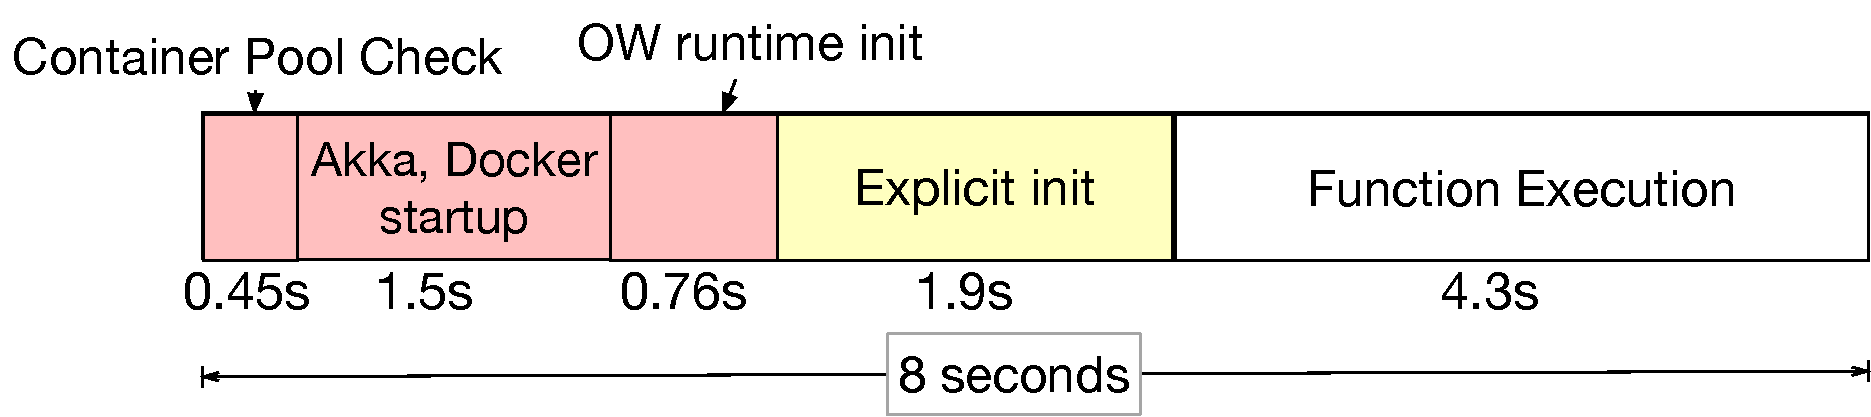
\includegraphics[width=0.8\textwidth]{faascache/faas-keepalive-20/figures/ow-timeline.pdf}
  \caption{Timeline of function execution and sources of cold-start delay in OpenWhisk for an ML inference application.}
  \label{fig:timeline}
\end{figure}


\noindent \textbf{Function Initialization.}
%\noindent \textbf{Function Initialization.}
%
%Optionally, applications may also use custom code to initialize and pre-warm the container 
%rev1 first and last line 
%Explicit
Function initialization refers to function-specific code for downloading and resolving code and data dependencies, which can be run before actual function execution (explicit-init component in Figure~\ref{fig:timeline}). 
For example, this can be used for downloading data dependencies ahead of time such as large neural network models for inference, or for runtime initialization such as downloading and importing package dependencies (e.g., Python packages). 
%The second technique for reducing the cold-start overhead is to explicitly initialize functions before running  them, and resolving most of the function's code and data dependencies during the initialization phase. 
%
An example of function initialization is shown in Figure~\ref{fig:lambda-example}, which shows a pseudo-code snippet of a function that performs machine learning inference on its input. 
For ML inference, the function downloads an ML model and initializes the TensorFlow ML framework (lines  5 and 6). 
If the function's container is kept alive, then invocations of the function do not need to run the expensive initialization code (lines 2--6). 
%Thus, the execution latency of functions can be minimized with a combination of careful function initialization and keeping the containers alive. 
% too broad a conclusion here...


% \footnotesize
\begin{figure}
\begin{lstlisting}[language=Python, numbers=left, frame=single, basicstyle=\footnotesize\sffamily, columns=fullflexible, xleftmargin=10.0ex, xrightmargin=10.0ex]
#Initialization code 
import numpy as np 
import tensorflow as tf
  
m = download_model('http://model_serve/img_classify.pb')
session = create_tensorflow_graph(m) 
  
def lambda_handler(event, context):
     #This is called on every function invocation 
     picture = event['data']
     prediction_output = run_inference_on_image(picture) 
     return prediction_output 
   \end{lstlisting}
   %\vspace*{\myfigspace}
   \caption{Initializing functions by importing and downloading code and data dependencies can reduce function latency by hiding the cold-start overhead.}
   \label{fig:lambda-example}
   %\vspace*{\myfigspace}
\end{figure}


% The function cold-start overhead includes both the execution environment initialization and the
\begin{comment}
Explicit initialization allows functions to be pre-warmed, and can be used to reduce the cold-start overhead. 
However, explicit initialization is not common---our empirical investigation into FaaS benchmarks~\cite{kim_functionbench_2019} and official examples showed that applications do not use this functionality. 
Nevertheless, it can be a powerful technique to amortize expensive operations such as package imports and downloading data dependencies. 
Explicit initialization can thus increase the effectiveness of keep-alive. 
However because it is not ubiquitous, we assume it is \emph{optional}, and our keep-alive and provisioning techniques work with and without it. 
\end{comment}


\noindent \textbf{Workload Diversity and Dynamism.}
%
Designing keep-alive policies is not trivial due to the highly diverse and expanding range of applications that are using FaaS control planes.
%This is in tradeoffs category. 
Conventionally, FaaS has been used for hosting web services, which is attractive because of the pay-per-use properties. 
Event handling functions for web responses typically have a small memory footprint but require low execution latency. 
Increasingly, FaaS is also being used for ``heavy'' workloads with high memory footprint and large initialization overheads such as highly parallel numerical computing (such as matrix operations~\cite{jonas2017occupy}, scientific computing~\cite{shankar2018numpywren}, and machine learning~\cite{akkus_sand_2018}. 
The diversity of FaaS applications also results in a wide range of function memory footprints, running times, and initialization times, as seen in Table~\ref{tab:workloads}.  
Keep-alive policies must therefore balance the resource footprint of the containers with the benefits of keeping containers alive---and do so in manner that is applicable across a wide range of applications. 


Furthermore, FaaS workloads show a high degree of dynamism and temporal effects. 
The Azure function~\cite{shahrad_serverless_2020} trace shows sharp diurnal effects: the function arrival rate is about $2\times$ higher during the peak periods compared to the average. 
Function workloads are also heavy-tailed: a few ``heavy hitting'' functions are invoked much more frequently than others or consume a larger amount of computing resources, often by 2 or 3 orders of magnitude. 


\subsection{Policy Goals and Considerations}


The primary goal of keep-alive is to reduce the initialization and cold-start latency, by keeping functions alive for different durations based on their characteristics. 
% Servers that run these functions are heavily multiplexed, and run hundreds of short lived functions concurrently. %backend FaaS servers?
% too sudden 
Because servers run hundreds of short lived functions concurrently, keep-alive policies must be generalizable and yield high server utilization. 
Functions can have vastly different characteristics, and keep-alive polices must work efficiently in highly dynamic and diverse settings. % (Table~\ref{tab:workloads}). 
We use the following characteristics of functions for keep-alive policies.


The \textbf{initialization time} of functions can vary based on the code and data dependencies of the function.  
For example, a function for machine learning inference may be initialized by importing large ML libraries (such as TensorFlow, etc.), and fetching the ML model, which can be hundreds of megabytes in size and take several seconds to download. 
Functions also differ in terms of their \textbf{total running time}, which includes the initialization time and the actual execution time. 
Again, functions for deep-learning inference can take several seconds, whereas functions for HTTP servers and microservices are extremely short-lived (few milliseconds). 
The \textbf{resource footprint} comprises of the CPU, memory, and I/O use, and also differs widely based on the application's requirements. 
Finally, functions have different \textbf{frequencies} and invocation rates. Some functions may be invoked several times a second, whereas other functions may only be invoked rarely (if they are used to serve a very low-traffic web-site, for instance). 

% \begin{figure}[t]
%   \centering
%   \vspace*{\myfigspace}
%   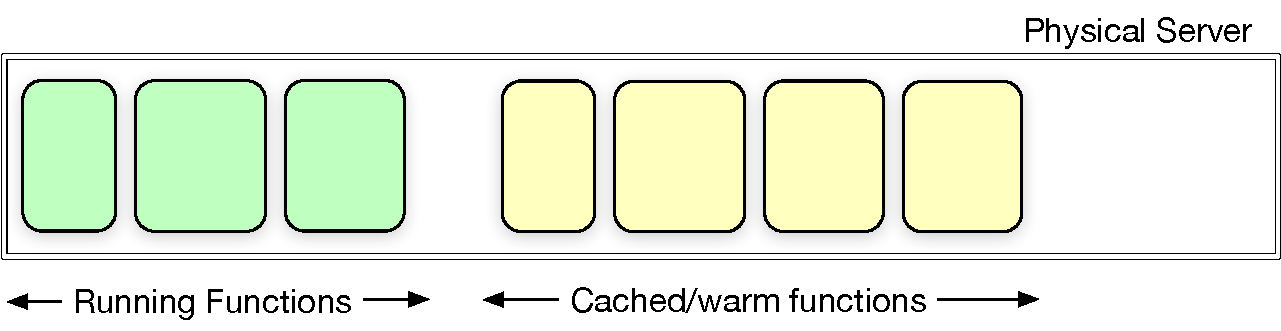
\includegraphics[width=0.4\textwidth]{../graphs/faas.pdf}
%   \vspace*{\myfigspace}
%   \label{fig:runwarm}
%   \caption{Server resources are consumed by running and warm containers.}
%     \vspace*{\myfigspace}
% \end{figure}


Because server resources are finite, it is important to prioritize functions which should be kept alive, based on the aforementioned characteristics. 
A function which is not popular and is unlikely to be called again in the near future, sees little benefits from keep-alive, and wastes server memory. 
%In fact, keeping such functions alive consumes valuable server computing resources for no gain in efficiency. %energy.. hmm
%Thus, keep-alive policies should prioritize popular functions. 
Similarly, the resource consumption of the functions is also important: since keeping large-footprint functions alive is more expensive than smaller functions, smaller functions should be preferred and kept alive for longer. 
Finally, functions can also be prioritized based on their initialization overhead, since it is effectively wasted computation.

% This paragraph is key. Different priorities and there is no one single ranking scheme for keepalive... 
The problem of designing keep-alive policies is complicated by the fact that functions may have vastly different keep-alive priorities for the different characteristics.
Consider a function with a large memory footprint (like those used in ML inference), high initialization overhead, and a low popularity.
Such a function should have a low keep-alive priority due to its size, high priority due to large initialization overhead, and a low priority due to its low popularity.
Thus, keep-alive policies must carefully balance all the different function characteristics and prioritize them in a coherent manner. 


% This still reads like making a case. But its only two sentences and bears repeating?
Current FaaS systems have shirked from this challenge and use primitive keep-alive policies that are not designed with the diversity and dynamism in mind. 
FaaS frameworks such as OpenWhisk, keep all functions alive for a \emph{constant} period of time (10 minutes). 
This is agnostic to different function characteristics such as resource footprint and initialization overheads, and only loosely captures popularity. 
More principled approaches are needed, which we provide next. 



%%% Local Variables:
%%% mode: latex
%%% TeX-master: "paper"
%%% End:



%%%%%%%%%%%%%%%%%%%%%%%%%%%%%%%%%%%%%%%%%%%%%%%%%%%%%%%%%%%%
\section{Caching-based Keep-Alive Policies}
\label{sec:cache-keep-alive}

%%%%%%%%%%%%%%%%%%%%%%%%%%%%%%%%%%%%%%%%%%%%%%%%%%%%%%%%%%%%

%\paragraph{Keep-alive is Equivalent to Caching.}
%\vspace*{\subsecspace}

Formulating a keep-alive policy that balances priorities based on its competing characteristics (memory footprint, frequency, initialization time, and execution time) of functions seems daunting. 

\begin{comment}
% \vspace*{-6pt}
\begin{framed}
  \vspace*{-6pt}
  \noindent \emph{The central insight of this paper is that keeping functions alive is equivalent to keeping objects in a cache.}
  \vspace*{-6pt}
\end{framed}
\vspace*{-2pt}
\end{comment}
%The problem of what functions to keep alive and for how long, is equivalent to what objects to cache. 

\noindent Keeping a function alive reduces its effective execution (or response) latency, in the same way as caching an object reduces its access latency. 
When all server resources are fully utilized, the problem of which functions \emph{not} to keep alive is equivalent to which objects to \emph{evict} from the cache. 
The high-level goal in caching is to improve the distribution of object access times, which is analogous to our goal of reducing the effective function latencies. 


This caching analogy provides us a framework and tools for understanding the tradeoffs in keep-alive policies, and improving server utilization. 
%The problem of cache eviction in object caching is a thoroughly studied for a wide range of constraints, systems, and environments. 
Caching has been studied a in wide range of contexts and many existing caching techniques can be applied and used for function keep-alive. 
Our insight is that we can use classic observations and results in object caching to formulate equivalent keep-alive policies that can provide us with well-proven and sophisticated starting point for understanding and improving function keep-alive.  


In the rest of this section, we will show how cache eviction algorithms can be adapted to keep-alive policies.
Caching systems typically seek to improve hit ratios (the fraction of accesses that are cache hits).
However, focusing on hit-rates alone does not necessarily translate to improved \emph{system} level performance if the objects have different sizes and miss costs.
For instance, caching all small objects may yield a high hit ratio, but the infrequent misses of larger objects results in higher miss costs and poor system throughput. 
Therefore, we will also focus on minimizing the overall cold-start overhead, which is equivalent to the ``byte hit ratio'' used in caching systems.



% We assume that each function in its own container.
% When the function is ``registered'', this container image is created.
% Multiple concurrent invocations to the same function are possible, but each invocation is in its own container.
% Containers are in one of two states. Either running the function, or are idling when they are being kept warm. 
% When a function is called by the user, if a corresponding container is ``free'', then it is used to run the function.
% Otherwise, a new container is instantiated.

% When a container is launched, the initilization code runs.
% Depending on the application and the FaaS platform, the amount of initilization can be different.
% For example, a truly ``stateless'' function will include all required dependencies on every invocation.
% In any case, there is some initilization and start-up overhead, which consumes 


% While any caching/eviction algorithm can be used with the help of this analogy after the mapping, the algorithm must be cognizant of the different resource footprints and access frequencies and execution latencies of different functions.
% %
% The greedy dual approach is a good mapping, which we use below. 

%\vspace*{\subsecspace}
\subsection{Greedy-Dual Keep-Alive Policy}
\label{subsec:gdsf}

While many caching techniques can be applied to the function keep-alive policies, we now present one such caching-inspired policy that is simple and yet captures all function characteristics and their tradeoffs.
Our \textbf{GDSF} policy is based on Greedy-Dual-Size-Frequency object caching~\cite{gdsf}, which was designed for caches with objects of  different sizes, such as web-proxies and caches. 
Classical caching policies such as LRU or LFU do not consider object sizes, and thus cannot be completely mapped to the keep-alive problem where the resource footprint of functions is an important characteristic. 
As we shall show, the Greedy-Dual approach provides a general framework to design and implement keep-alive policies that are cognizant of the  frequency and recency of invocations of different functions, their initialization overheads, and sizes (resource footprints). 


Fundamentally, our keep-alive policy is a function \emph{termination} policy, just like caching focuses on eviction policies.  
Our policy is resource conserving: we keep the functions warm whenever possible, as long as there are available server resources. 
This is a departure from current constant time-to-live policies implemented in FaaS frameworks and public clouds, that are \emph{not} resource conserving, and may terminate functions even if resources are available to keep them alive for longer. 

%We assume that each functions is deployed in a container, and o
Our policy decides which container to terminate if a new container is to be launched and there are insufficient resources available. 
The total number of containers (warm + running) is constrained by the total server physical resources (CPU and memory). 
We compute a ``priority'' for each container based on the cold-start overhead and resource footprint, and terminate the container with the lowest priority.
%
%Below, we describe our termination policy in detail.


%\noindent \textbf{Execution model.}
%Assume that there are $n$ different functions.
%
%We assume that each function runs in its own container.
%
%Each function can have multiple independent and concurrent instantiations, and hence containers. 
%
%At any instant of time, each container is either running a function, or is being kept alive/warm. 
%

%What is the point of this? 
%Assume that a  function $i$ has a initialization or startup time of $s_i$. 
%Once initialized, the running time of the function is  $r_i$, and thus total running time for the cold-start case is $s_i + r_i = T_i$.  
%When executing on a warm container, the time is simply $w_i$.
%


%Let $m_i$ be the memory footprint of the function.


%The total number of containers (warm + running) is constrained by the total server physical resources (cpu and memory). 
%Each container has a resource footprint, which we also call the \emph{size} of the container, denoted by $\mathbf{d_i}$.
%The size may be a multi-dimensional resource vector comprising of the CPU, memory, and I/O resources used by the running or warm container.
%In most scenarios, the number of containers that can run is limited by the physical memory availability, since CPUs can be multiplexed easily, and memory swapping can result in severe performance degradation.
%Thus for ease of exposition, we can consider only the container \emph{memory} use as the size, instead of a multi-dimensional vector. 


\noindent \textbf{Priority Calculation.} 
The GDSF keep-alive policy is based on Greedy-Dual  caching~\cite{young_gd_orig_94}, where objects may have  different eviction costs. 
%
For each container, we assign a \emph{keep-alive priority}, which is computed based on the frequency of function invocation, its running time, and its size:
%
% The priority is given by:
\vspace*{-7pt}
\begin{equation}
  \vspace*{-3pt}
  \text{Priority} = \text{Clock} + \frac{\text{Freq} \times \text{Cost}} {\text{Size}}
    \label{eq:prio-prop}
\end{equation}
%
% 

On every function invocation, if a warm container for the function is available, it is used, and its frequency and priority are updated.
Reusing a warm container is thus a ``cache hit'', since we do not incur the initialization overhead. 
When a new container is launched due to insufficient resources, some other containers are terminated based on their priority order---lower priority containers are terminated first. 
We now explain the intuition behind each parameter in the priority calculation:



\noindent \textbf{Clock} is used to capture the recency of execution.
We maintain a ``logical clock'' per server that is updated on every eviction. 
Each time a container is used, the server clock is assigned to the container and the priority is updated.  
Thus, containers that are not recently used will have smaller clock values (and hence priorities), and will be terminated before more recently used containers. 

% Didnt understand the need for this
%Although this is termination, it is something about clock. so here. 
Containers are terminated only if there are insufficient resources to launch a new container and if existing warm containers cannot be used.  
Specifically, if a container  $j$ is terminated (because it has the lowest priority), then $\text{Clock} = \text{Priority}_j$.
All subsequent uses of other, non-terminated containers then use this clock value for their priority calculation.
In some cases, \emph{multiple} containers may need to be terminated to make room for new containers.
If $E$ is the set of these terminated containers, then $\text{Clock} = \max_{j \in E}{\text{Priority(j)}}$

We note that the priority computation is on a per-container basis, and containers of the same function share some of the attributes (such as size, frequency, and cost). 
However, the clock attribute is updated for each container individually. 
This allows us to evict the oldest and least recently used container for a given function, in order to break ties. 


\noindent \textbf{Frequency} is the number of times a given function is invoked.
A given function can be executed by multiple containers, and frequency denotes the \emph{total} number of function invocations across all of its containers. 
The frequency is set to zero when all the containers of a function are terminated.
The priority is proportional to the frequency, and thus more frequently executed functions are kept alive for longer. 
%
%This is a departure from object caching, where each object is distinct. In our case, because of concurrent executions of functions, multiple containers for the same function may exist, and we thus take into account all the 
%


\noindent \textbf{Cost} represents the termination-cost, which is equal to the total initialization time. 
This captures the benefit of keeping a container alive and the cost of a cold-start. 
% There are other cost formulations also, such as $c/T$ etc that capture the ratio, that yield different policies.
The priority is thus proportional to the initialization overhead of the function. 



\noindent \textbf{Size} is the resource footprint of the container. 
%If we only care about the memory size, then we can simply use a single dimensional metric $m_i$ to denote the size.
The priority is inversely proportional to the size, and thus larger containers are terminated before smaller ones. 
In most scenarios, the number of containers that can run is limited by the physical memory availability, since CPUs can be multiplexed easily, and memory swapping can result in severe performance degradation.
Thus, for ease of exposition and practicality, we consider only the container \emph{memory} use as the size, instead of a multi-dimensional vector. 


We can also use multi-dimensional resource vectors to represent the size, in which case we convert them to scalar representations by using the existing formulations from multi-dimensional \emph{bin-packing.}
For instance, if the container size is $\mathbf{d}$, then the size can be represented by the magnitude of the vector $||\mathbf{d}||$.
Other size representations can also be used.
A common technique is to normalize the container size by the physical server's total resources ($\mathbf{a}$), and then compute the size as $\sum_j \frac{d_j}{a_j}$ where $d_j, a_j$ are the container size and total resources of a given type (either CPU, memory, I/O) respectively.
Cosine similarity between $\mathbf{d}$ and $\mathbf{a}$ can also be used, as is widely used in multi-dimensional bin-packing.  


\noindent \textbf{FaaS-specific considerations.}
The application of cache eviction algorithms to FaaS keep-alive is fairly straight-forward.
The various inputs Greedy-Dual (memory size, cold-start time, frequency) are available once a function has finished execution, and thus the keep-alive policy is completely online. 
Our policy calculates eviction priorities at the function level, but evicts at the container level. 
Recall that a particular function may have multiple containers associated with concurrent function invocations. 
We assume that all containers of a function are identical, i.e., they have the same initialization cost, footprint, etc. 
Thus, any one of the identical containers can be evicted. 



\subsection{Other Caching-Based Policies}
\label{subsec:variants}

The Greedy-Dual approach also permits many specialized and simpler policies.
For instance, allowing for different parameters in Equation~\ref{eq:prio-prop} results in different caching algorithms.
If only the access clock is used as a priority, and other parameters are ignored, then we get \textbf{LRU}, with its ease of analysis and generality which has been well established with over half a century of empirical and analytical work. 
Using only frequency yields \textbf{LFU.}
Similarly, a size aware keep-alive policy can be obtained by using 1/size as the priority, which would be useful in scenarios where memory size is at a premium. 


Other size-aware online algorithms with tight online theoretical guarantees can also be applied.
We also implement the \textbf{LANDLORD}~\cite{young2002line} algorithm, which can be understood as a variant of the Greedy-Dual approach.
Landlord also considers the frequency, size, and initialization cost of functions.
When the server is full and some container is to be evicted, a ``rent'' is charged from each function based on its size and initialization cost (specifically, it is equal to $\min(\frac{\text{initialization cost}}{\text{size}})$.
This subtly differs from Greedy-Dual-Size-Frequency: the decrease in priority is computed based on the state of all the cached containers, and not independently applied. 
Upon a function invocation, its containers get a ``credit'', and their priority is set to their initialization cost. 
The containers with the lowest credits are evicted. 
Landlord has appealing and well-proven properties of its online performance: its competitive ratio (the performance compared to an optimal \emph{offline} algorithm that knows future requests) has been well analyzed~\cite{young2002line}. 




%%% Local Variables:
%%% mode: latex
%%% TeX-master: "paper"
%%% End:


\section{Server Provisioning Policies} % Resource provisioning ?
\label{sec:provision}

Resource provisioning, i.e., determining the size and capacity of the servers for handling FaaS workloads, is a fundamental problem in serverless computing. 
In this section, we develop techniques that allocate the appropriate amount of resources to servers based on the characteristics of the function workloads. 
Resource provisioning policies must consider the rate of function invocations, the resource footprints of the functions, and the inter-arrival time between function invocations. 
To handle the interplay and tradeoffs between these factors, we use similar principles for provisioning that we used for developing our keep-alive policies. 
% Previous three lines are a bit verbose and can be compressed to 2, but ok.. 
% rev 1 
In case FaaS workloads are co-located with other applications such as long-running containers and VMs, our provisioning policies can also be used to determine the resource allocation of the combined running and warm function pool. 

The fundamental challenge underlying resource provisioning for FaaS workloads is the performance vs. resource allocation tradeoff. 
Running a workload on large servers/VMs provides more resources for the keep-alive cache, which reduces the cold-starts and improves the application performance. 
However, we must also be careful to not \emph{overprovision}, since it leads to wasted and underutilized resources.
Additionally, since function workload can be dynamic, resource provisioning must be \emph{elastic}, and be able to dynamically scale up or down based on the load. 
We therefore present a \emph{static} provisioning policy that determines the server memory size for a given function workload, and then develop an elastic-scaling approach for handling workload temporal dynamics. 

\subsection{Static Provisioning}
\label{subsec:static}

In Section \ref{sec:bg}, we have seen how keeping function containers warm in a keep-alive cache can help mitigate the cold-start overheads. 
The effectiveness of any keep-alive policy depends on the size of this keep-alive cache, and thus the server resources available, i.e., the server size. 
Our \emph{static} provisioning policy thus selects a server size for handling a given workload. 
% Not peak, since that would be infinite sized. 90 percentile, but we dont do that. 
We want to optimize the resource provisioning to avoid over and under provisioning, both of which are detrimental to cost and performance respectively. 


Having established that keep-alive policies are equivalent to cache eviction in the previous section, we now extend the use of the caching analogy further, to develop a caching-based provisioning approach. 
We claim that the performance vs. resource availability tradeoff of serverless functions can be understood and modeled using cache hit (or miss) ratio curves.
%
Hit-ratio curves are widely used in cache provisioning and modeling, since they give insights into cache performance at different sizes. 
%The performance of caches is typically modeled by constructing a hit ratio curve, which determines the hit-ratio at different cache sizes.
%The ``optimum'' cache size is based on the marginal utility or the slope of the hit ratio curve. 
%Due to temporal locality of object references, hit-ratio curves are typically long-tailed, which makes provisioning... ? 
Once a hit-ratio curve is obtained, it is used to provision the cache size based on system requirements. 
A common approach is to size the cache based on a target hit-ratio (say, 90\%). 
Alternatively, the slope of a hit-ratio curve can be understood to be the marginal utility of the cache, and a cache size that maximizes this marginal utility is picked.
This entails choosing a cache size which corresponds to the \emph{inflection point} of the hit-ratio curve. 


% We use a similar approach.
\noindent \textbf{Hit-ratio Curve Construction.}
We use a function hit-ratio curve for determining the percentage of warm-starts at different server memory sizes. 
The hit-ratio curve is constructed by using the notion of \emph{re-use distances.}
A function's reuse-distance is defined as the total (memory) size of the unique functions invoked between successive invocations of the same function.
For example, in the request \emph{reuse} sequence of \texttt{ABCBCA}, the reuse distance of function \texttt{A} is equal to \texttt{size(B) + size(C)}.
%
The \emph{distribution} of these reuse distances can yield important insights into the required cache size.
If the cache size is greater than the reuse distances, then there will be no cache misses. 
This can be generalized to find the hit-ratio at cache size $c$:   \vspace*{-5pt}
\begin{equation}
  \label{eq:hrc-rdd}
  \text{Hit-ratio}(c) = \sum_{x=0}^cP(\text{Reuse-distance} = x),
    \vspace*{-5pt}
\end{equation}
where the reuse distance probability is obtained by scanning the entire input function workload for all reuse sequences. 
Conveniently, the hit-ratio is the CDF (cumulative distribution function) of the reuse distances, which can be empirically determined based on all the computed reuse distances. 
We show one such hit-ratio curve constructed with reuse distances, for a representative sample of the Azure function workload in Figure~\ref{fig:hrc}. 
We can see that the hit-ratio curve of functions \emph{also} follows the classic long-tailed behavior: the hit-ratio steeply increases with cache size up to an inflection point, after which we see diminishing returns. 


This technique and observation informs our provisioning policy.
We construct a hit-ratio curve based on reuse distances, and size the server's memory based on the inflection point.
Alternatively, we can set a target hit ratio (say, 90\%), and use that to determine the minimum memory size of the server. 
%
Finding the reuse-distances for an entire trace can be an expensive, one-time operation, and takes $O(N*M)$ time where N is the number of invocations and M is the number of unique functions. 
However, sampling techniques such as SHARDS~\cite{shards} can be applied to drastically reduce the overhead, making this a practical and principled technique for resource provisioning. 



\begin{figure}[t]
  \centering
  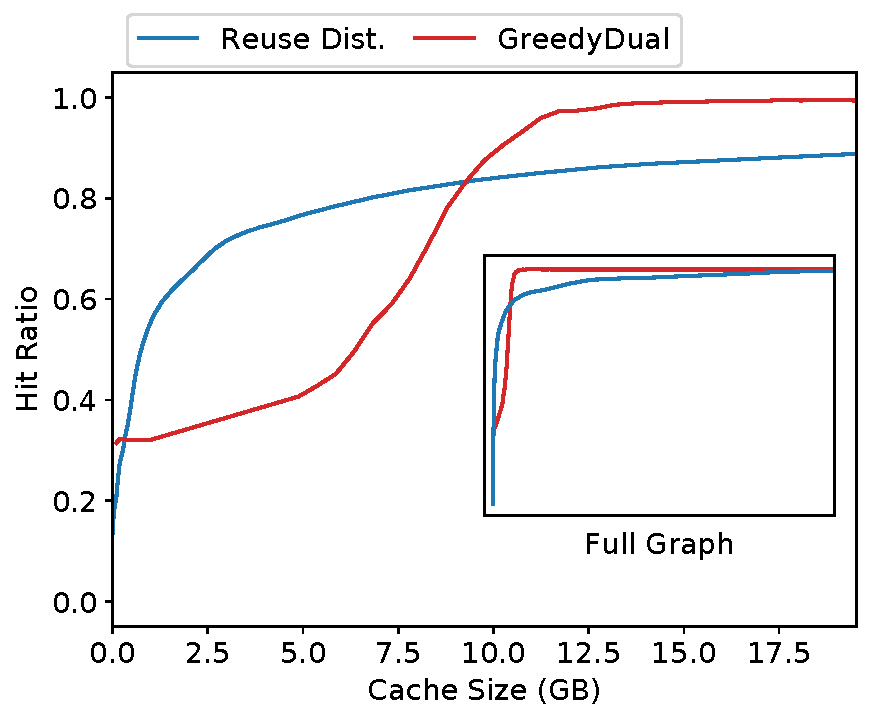
\includegraphics[width=0.5\textwidth]{faascache/faas-keepalive-20/graphs/rep-funcs-392/hit-ratio-392-b.pdf}
  \caption{Hit ratio curve using reuse distances show slight deviations from the observed hit ratios due to dropped requests at lower sizes, and concurrent executions at higher sizes.}
  \label{fig:hrc}
\end{figure}

\paragraph{Limitations of the Caching Analogy.}
The error in hit-ratios with the reuse-distance approach in Figure~\ref{fig:hrc} highlights an important facet where caching does not fully map to FaaS.
The main difference is due to the limitations on the concurrent execution of functions: 
caching deals with unique objects, whereas there can be  multiple containers for a function. 
%
At lower cache sizes, a high miss rate results in higher server load, and hence a higher number of dropped requests, that the classical reuse-distance approaches do not capture.
If all warmed containers of a function are in use, then a new invocation results in a cold-start---which would be counted as a cache ``hit''.
Thus at lower sizes, the real hit-ratio is lower than the ideal. 
At larger sizes, \emph{multiple} containers corresponding to concurrent invocations of a function will be present, which results in a deviation from the hit-rate curve. 
%: which is again different from the caching model where objects are unique. 
Reconciling these differences is an interesting area of future work. %but does not impact our work significantly. 
However, we note that hit-ratio curves are only used for coarse-grained allocation, and small deviations result in slight under or over provisioning. 
Moreover, our dynamic allocation policy described next can reduce these errors using proportional control. 

%\prat{Difference in two curves: could be because of multiple containers for a function, which is different from caching. So for larger cache sizes, the hit-ratio is higher. For lower sizes: it is lower because of dropped requests and not being able to handle the concurrent accesses which is not true with caching. So this is some sort of a negative result, or an area for future work.}


\subsection{Elastic Dynamic Scaling}
\label{subsec:dynamic}

We also use the hit-ratio curve approach for a \emph{dynamic} auto-scaling policy that adjusts the server size based on workload requirements. 
%
We assume that the FaaS server backend is running functions as containers either inside a virtual machine (VM), or is sharing the physical server with other cloud applications. 
In either case, it is important to be able to reclaim unused keep-alive cache resources and reduce its footprint, in order to increase the efficiency of the cloud platform. 

Our vertical elastic scaling policy is simple and is intended to demonstrate the efficacy of a general caching based approach. 
We implement a  proportional controller~\cite{pid-wiki} which periodically adjusts the VM memory size based on the rate of cold-starts.  
Thus during periods of low rate of function invocations (i.e., arrival rate), the cache size can be reduced. 
This may \emph{increase} the miss-ratio---but we care about the cold-starts (i.e., misses) per second, which is product of miss-ratio and invocations per second.
Our controller monitors the arrival and cold-start rate, and uses the hit-ratio curve to decrease or increase VM size dynamically. 
We use VM resource deflation~\cite{deflation-eurosys19} to shrink or expand the VM by using a combination of hypervisor level page swapping, or guest-OS memory hot-plug and unplug. 


Assume that we have a target miss speed (number of cold-starts/misses per second).
For instance, this target value can be a product of the desired hit-ratio, $h$, and the average function arrival rate for the entire workload trace, $\bar{\lambda}$. 
Periodically, we monitor the exponentially smoothed arrival rate $\lambda$, and the observed miss speed.
Our proportional controller adjusts the cache size in order to reduce the difference between the actual vs. target miss speed.
This error is used to compute the new \emph{miss rate}, $m$, and the associated cache size $c'$ as follows:
\begin{align}
  \label{eq:dyn}
%  m & = \frac{\bar{\lambda}}{\lambda}*h \\
  \text{HR}(c') & = 1-m = 1 - h\frac{\bar{\lambda}}{\lambda}
\end{align}

\noindent The new cache size $c'$ is then determined by inverting the hit-rate function $\text{HR}$.
Our vertical scaling controller is designed for coarse-grained VM size adjustments, and only tracks the workload at time granularities of several minutes. 
Our intent with this policy is to not be overly aggressive with the capacity changes, but only to capture the coarse diurnal effects. 
Therefore, we use a large error deadband: the cache size is only updated if the error is more than 30\%. 
%More sophisticated, predictive and reactive auto-scaling policies from web-clusters~\cite{gandhi2012autoscale} can be also be adapted. 
Finally, the memory scaling can also be combined with cpu auto-scaling based on the function arrival rate, using classical predictive and reactive auto-scaling techniques found in web-clusters~\cite{gandhi2012autoscale}. 

\paragraph{Online adjustments.} %rev1
Our policies rely on the \emph{aggregate} function characteristics, which is used for constructing the hit-ratio curve. 
Once done, the traffic intensity (invocations per second) can change.
We primarily assume that the probability distribution of function characteristics such as their frequency and size, does not significantly change.
However, our dynamic scaling policy can adjust to changes in the traffic intensity (invocations per second). 
In other words, we assume that the future traffic is going to be similar to the past, which is the basis of the timeseries-forecasting based policies (such as in ~\cite{shahrad_serverless_2020}), and is the fundamental principle underlying caching in general. 
%
Our provisioning policies are not completely online, since they have a preparation phase for constructing the hit-rate curves. 
A ``drift'' in function characteristics is fixed by periodically updating the hit-ratio curve, which we currently do once per week. 
Online hit-ratio curves can also be constructed, and adapting techniques such as ~\cite{zhang2020osca} is part of our future work.





% Let the exponentially smoothed arrival rate of functions be $\lambda$. 

% The hit-ratio curve constructed for the static provisioning is applicable for the overall workload for the average arrival rate $\bar{\lambda}$.
% For the elastic scaling, we monitor the exponentially smoothed arrival rate, $EWMA(\lambda)$, and scale up or down if it is more than one standard deviation from $\bar{\lambda}$. 
% If $\lambda < \bar{\lambda}$, we scale the server's memory down by $\delta(m)$, which is determined based on the cache hit ratio curve to meet the average or the set number of misses per second. 


% Let current cache size be c, and load be $\lambda$.
% In general, the misses per second is given by $m = (1-HR(c))\lambda$.
% The goal is to keep this constant, that is $m = \bar{m}$.
% If the new cache size is $c'$, then we have: $(1-HR(c'))\lambda  = (1-HR(c))\bar{\lambda}$
% \begin{equation}
%   \label{eq:dyn} 
%   HR(c') = 1- \dfrac{(1-HR(c))\bar{\lambda}}{\lambda} 
% \end{equation}
% We use the hit-rate curve to thus find $c'$ that yields the hit-rate on the right hand side of the above equation.  

% tgt-miss-rate = avg-lambda/lambda*miss-ratio 


%%% Local Variables:
%%% mode: latex
%%% TeX-master: "paper"
%%% End:


\section{Implementation}

We have implemented the keep-alive and the provisioning policies as part of our FaasCache framework built on top of OpenWhisk (Figure~\ref{fig:sys}). 

\begin{figure}[t]
  \centering
  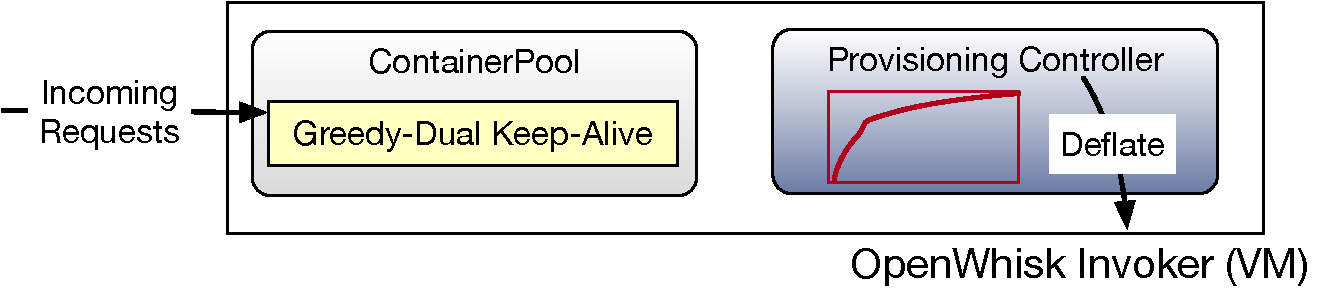
\includegraphics[width=0.95\textwidth]{faascache/faas-keepalive-20/figures/faascache.pdf}
  \caption{FaasCache system components. We build on OpenWhisk and augment it with new keep-alive policies and a provisioning controller. }
  \label{fig:sys}
\end{figure}

\noindent \textbf{Keep-Alive.}
FaasCache replaces the default OpenWhisk TTL-based keep-alive policy with the Greedy-Dual-Size-Frequency approach. 
For each initialized container, we assign and maintain the keep-alive prioritized ContainerPool, which is only a 100-line Scala modification. 
%Initialized containers are managed by the ContainerPool.
%\emph{Interesting aspects of priority calculation?} How is size, clock, frequency, cost, etc. computed? How does the impl differ from the idealized description? 
Each invocation of a function (OpenWhisk action) in ContainerPool records the launch time and when results are returned.


If the container was prewarmed before the invocation arrived, we record it as the function's warm runtime.
For new functions, the initialization overhead is captured and assumed to be the worst-case runtime until a warmed invocation is recorded. % is approximated as the minimum overhead of Docker and OpenWhisk's Python runtime initialization.
In the subsequent invocations, the initialization overhead is computed by subtracting the cold from the warm time. 
%Otherwise it was a cold start.
%The maximum cold and warm runtimes are kept per function to compute the priority.
%Size is simply the number of megabytes of memory OpenWhisk preallocates to the action's container, and
The function's frequency and clock value are updated with each request.
If the last container of a function is evicted, its cold and warm runtimes are stored and used to compute priority for its future invocations. 
%
To preserve the invocation fast-path, the ContainerPool is not kept sorted by priority. 
%Priorities are computed when an eviction needs to be made to reclaim memory.
Instead, it is sorted by priorities only during evictions, when the lowest priority container(s) are terminated.
%
We batch eviction operations to optimize the slow-path: we evict multiple containers to reach a certain free resource threshold (1000 MB is the current default). 

%rev 1
In the future, we intend to implement a similar design that is found in the Linux kernel page eviction. A separate thread (analogous to kswapd) can be used to periodically sort the containerpool list and asynchronously evict containers, so that eviction is not on the critical path. 

%All of an action's containers share one priority, regardless of the last time each ran an invocation.

% \prat{How are the values inferred?}
% New functions always replace old functions in the ContainerPool, so the priority of newly inserted containers doesn't matter. 
% After the second invocation of a function, its initialization overhead is inferred as the difference between the cold (first) and warm (subsequent) invocations. 
% Memory usage of the container is gathered via {\em Docker stats?\/}.



\noindent \textbf{Provisioning.}
For the static provisioning, we compute the reuse distance distribution for a given workload trace, and assume stationarity --- that it will be applicable on similar future workloads. 
We compute the reuse distances conventionally, by examining all reuse-sequences.
The dynamic provisioning controller runs periodically (every 10 minutes), to deflate or inflate the VM size, if the cold start rate deviates from the target significantly (by more than 30\%).
When the VM has to be shrunk, we use cascade deflation~\cite{deflation-eurosys19}.
We shrink the ContainerPool first, and reclaim the free memory using guest OS-level memory hot-unplug and hypervisor-level page swapping. 
%This approach is based on cascade deflation proposed in~\cite{deflation-eurosys19}. 

%Optimizations such as SHARDS that can significantly reduce the running time by sampling a small fraction of the functions, were found to be inadequate due to the wide disparity in the function sizes.
%The efficacy of sampling based techniques like SHARDS has mainly been empirically established only for fixed-sized objects. 


\noindent \textbf{Keep-alive Simulator.}
We have implemented a trace-driven discrete event simulator for implementing and validating different keep-alive policies.
Our simulator is written in Python in about 2,000 lines of code, and implements the various variants described in Section~\ref{subsec:variants}. 
It allows us to determine the cache hit ratios and the cold start overheads for different workloads and memory sizes.
Additionally, it also implements the static and dynamic provisioning policies for adjusting server size.

%%% Local Variables:
%%% mode: latex
%%% TeX-master: "paper"
%%% End:


\section{Experimental Evaluation}

% section Evaluation
\label{sec:eval}


We now present the experimental evaluation of our caching-based keep-alive technique by using function workload traces and serverless benchmarks.
Our goal is to investigate the effectiveness of these techniques under different workload and system conditions. 


\begin{figure*}
  \centering
\subfloat[ Representative functions.     \label{fig:rep-trace-exec}]
{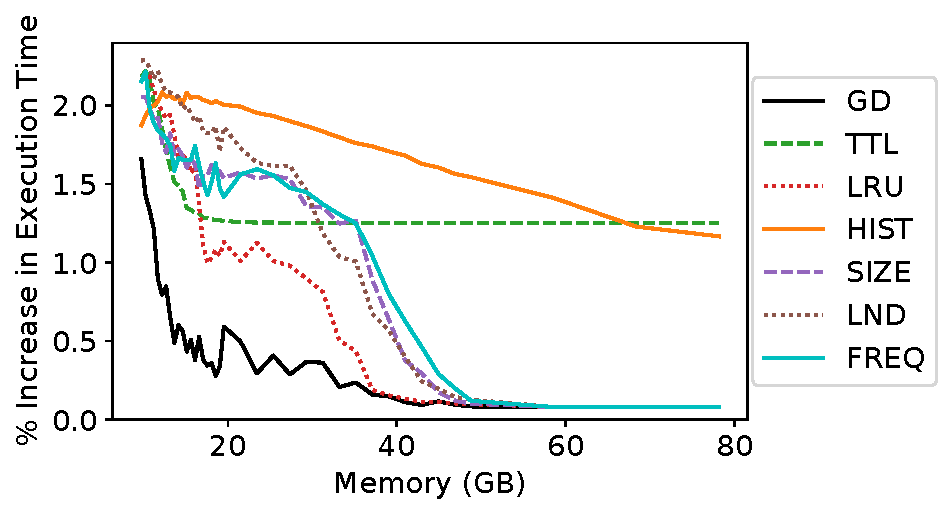
\includegraphics[width=0.37\textwidth]{faascache/faas-keepalive-20/graphs/rep-funcs-392/exec_inc_mem-392-legend.pdf}}
  \hfill 
    \subfloat[Rare functions.     \label{fig:rare-trace-exec}]
{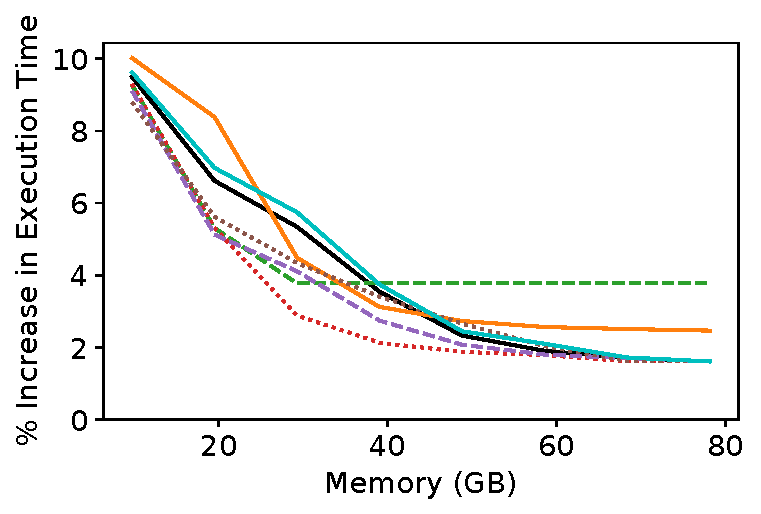
\includegraphics[width=0.3\textwidth]{faascache/faas-keepalive-20/graphs/rare-funcs-1000/exec_inc_mem-1000.pdf}}
\hfill 
  \subfloat[Random sampling.      \label{fig:random-trace-exec}] {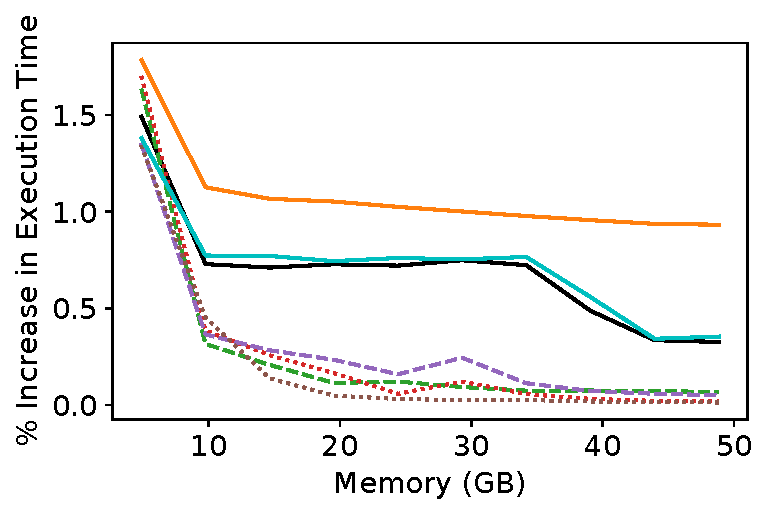
\includegraphics[width=0.3\textwidth]{faascache/faas-keepalive-20/graphs/random-funcs-200/exec_inc_mem-200.pdf}}
\caption{Increase in execution time due to cold starts for different workloads derived from the Azure function trace.}
\label{fig:exec-overheads-all}
\end{figure*}


\begin{figure*}[t]
  \centering
%  \vspace*{\myfigspace}
%  \begin{minipage}[c]{0.7\linewidth}
  \subfloat[Representative functions.\label{fig:rep-trace-cold}] {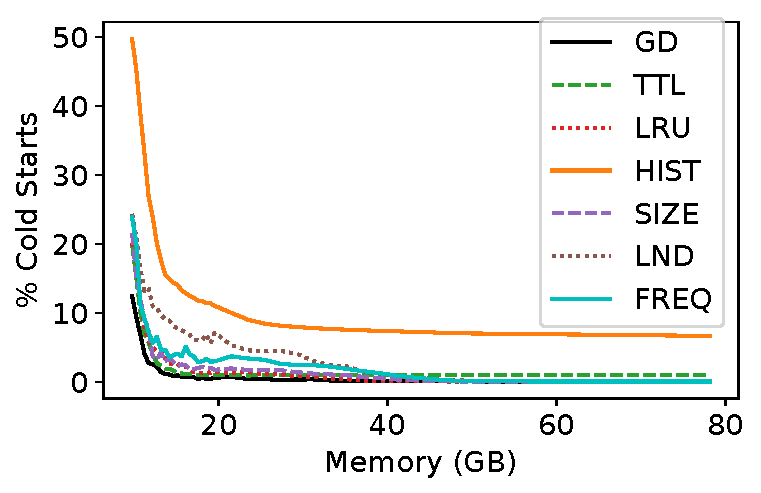
\includegraphics[width=0.33\textwidth]{faascache/faas-keepalive-20/graphs/rep-funcs-392/cold_drop_mem-392-legend.pdf}}
  \hfill
    \subfloat[Rare functions. \label{fig:rare-trace-cold}] {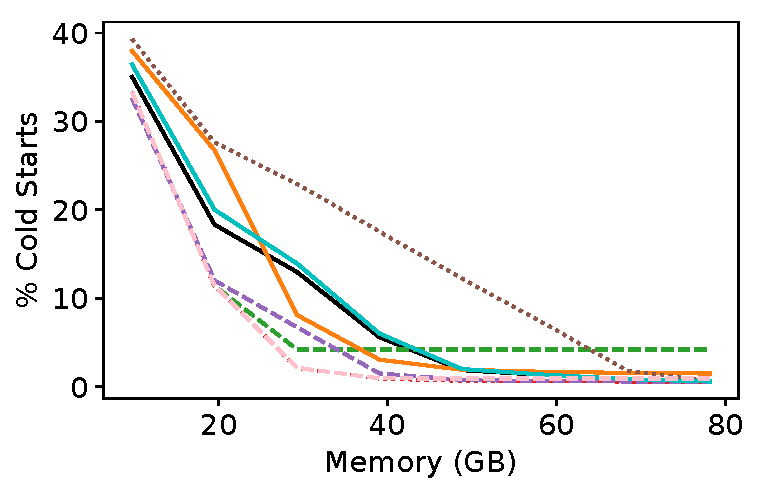
\includegraphics[width=0.33\textwidth]{faascache/faas-keepalive-20/graphs/rare-funcs-1000/cold_drop_mem-1000.pdf}}
  \hfill
  \subfloat[Random sampling. \label{fig:random-trace-cold}]
  {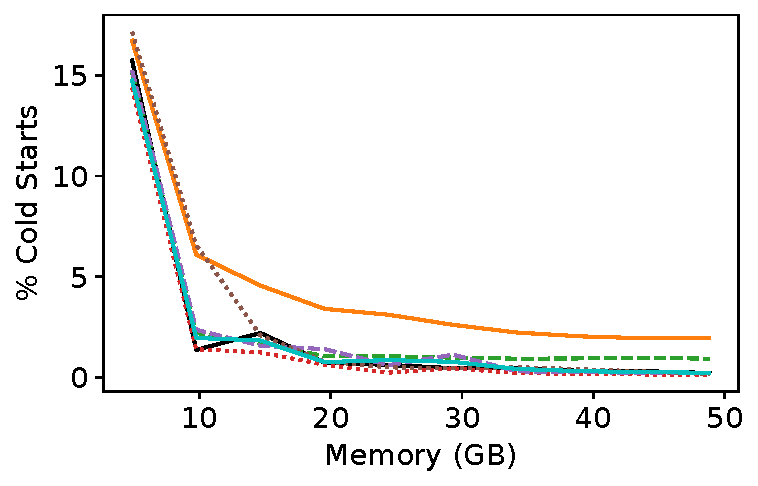
\includegraphics[width=0.33\textwidth]{faascache/faas-keepalive-20/graphs/random-funcs-200/cold_drop_mem-200.pdf}}
    \caption{Fraction of cold starts is lower with caching-based keep-alive. } % for different samples of the Azure function trace.}
      \label{fig:cold starts-all}
%    \end{minipage}
%    \hfill
%    \begin{minipage}[c]{0.29\linewidth}
 %      \begin{figure}
 %     \end{figure}
%    \end{minipage}
\end{figure*}


%%%%%%%%%%%%%%%%%%%%%%%%%%%%%%%%%%%%%%%%%%%%%%%%%%%%%%%%%%%%
\noindent \textbf{Setup, Workloads, and Metrics.}
%
For evaluating different keep-alive performance with different workload types, we use different trace samples from the Azure Function trace~\cite{shahrad_serverless_2020}, which contains execution times, memory sizes, and invocation-timestamps for more than 50,000 unique functions. 
Since our goal is to examine performance at a \emph{server} level, we use smaller samples of this trace for realistic server sizes, and replay them in our discrete-event keep-alive simulator. 
This also allows us to examine the behavior with different \emph{types} of workloads, which is important because our keep-alive policies are designed to be general and workload-agnostic.
We use the following three trace samples (more details in the Table~\ref{tab:trace-deets}): \\
\noindent \textbf{RARE:} A random sample of 1000 of the rarest, most infrequently invoked functions. These functions will usually result in cold starts under a classic 10 minute TTL.  \\
% mention 75% percentile detail?
\noindent \textbf{REPRESENTATIVE:} A sample of 400 functions, sampled from each quartile of the dataset based on frequency---yielding a more representative sample with higher function diversity. \\
\noindent \textbf{RANDOM:} A random sample of 200 functions.

% The FaasCache system is evaluated in Section~\ref{subsec:ow-eval}.
Functions from the FunctionBench~\cite{kim_functionbench_2019} suite are used for generating a realistic workload. 
A single server with 250 GB RAM and 48-core Intel Xeon Platinum 2.10 GHz CPUs is used for running all functions. The server is running modified OpenWhisk (i.e., FaasCache), and Ubuntu 16.04.5. 

\begin{table}
  \centering
  \caption{Size and inter-arrival time (IAT) details for the Azure Function workloads used in our evaluation.}
  \begin{tabular}{lrrr}
    \hline 
    Trace & Num Invocations & Reqs per sec & Avg. IAT \\
    \hline
    Representative & 1,348,162 & 190 /s & 5.4 ms \\
    Rare & 202,121 & 30 /s & 36 ms \\
    Random & 4,291,250 & 600 /s & 1.8 ms \\
    \hline
  \end{tabular}
  \label{tab:trace-deets}
\end{table}



\paragraph{Adapting the Azure Functions Trace.}
The format of the original Azure Function trace~\cite{shahrad_serverless_2020} requires some additional pre-processing and extrapolation for generating a workload.  
The full dataset consists of 14 days of function invocations, and billions of individual invocations. We use the first day's data, and do not consider functions that are never reused (i.e., with less than two invocations). 

The original trace provides memory consumption at the \textit{application} level---with the application made up of multiple functions.
Therefore, we evenly split the memory allocation between all functions in an application.
The dataset provides invocations in minute-wide buckets.
When injecting/replaying the workload, if there is only one invocation in a minute-bucket, it is injected at the beginning of the minute. 
For multiple invocations, they are equally spaced throughout the minute. 

%
The cold start overhead of each function is estimated as {\texttt maximum - average} runtime, and the execution times provided in the dataset are used for this computation. 
The dataset does not account for certain important sources of cold start overheads such as execution environment creation (e.g., Docker).
This unfortunately underestimates the cold start overheads.
However, because it applies uniformly to all functions, it preserves the relative performance of the different keep-alive policies, and does not affect the cache hit ratios. 
%

%These cold start overheads are generally constant, 

%This may not capture all the sources of cold start overhead such as the execution environment creation (e.g., Docker) and 

We are interested in two metrics: the cold start ratio; and the average increase in the execution time due to cold starts.
The increase in execution time is computed by averaging across all function invocations. 

%The latter captures the heterogeneity in function initialization overheads and invocation frequencies. 
%For estimating the time each function spends in explicit initialization, using the workload trace we subtract each functions' average runtime from its maximum runtime. 
%The dataset timings do not include provider overhead, so this initialization time is entirely due to application code.

%%
%Provider cold start overheads can be up to several seconds long, and take up the plurality of a function's execution time.
%Because the dataset does not include provider overhead, it is impossible to assign a realistic number to this cost.
%With these large penalties are not in our simulations, we therefore assume it as 0, but in reality the overhead is roughly constant.
%This causes the global increase in execution time to be smaller than it would be otherwise.
%Including a non-zero cold start cost would apply uniformly across all functions, and thus not change eviction priorities relative to one another.
%The cache hit ratio in Figure~\ref{fig:cold starts-all} would remain unchanged, and the Y-axis (the global increase in execution time) of Figure~\ref{fig:exec-overheads-all} would be scaled up relative to the chosen cold start overhead.
%%

% Using variable, real-world, times would require knowing or randomly assigning the runtime of functions, and would still require stochasticity as provider latency is not constant. 

% Not explaining this in the paper was our biggest “oops”: and there’s a few sources of confusion.
% Here is what we assumed: the dataset doesnt include container startup time, but the included function execution time captures both the function-initialization time (importing packages etc.), and the actual execution.
% So the assumption is that the Max execution time was due to this initialization overhead (which we include in the cold start overhead in our paper).
% The “time functions take to execute after they are ready to run” added to our confusion: we assumed this meant that it is the time when the control is transferred to the FaaS runtime inside the container: which would still incorporate all actual function initialization overheads.
% A contributing factor to making this assumptions was that most OpenWhisk applications do not have a strict explicit initialization, so it is in general not possible to know when a function is truly ready to execute non-idempotent code. 

% And so we end up with pretty small startup overheads, which can be seen from our Figure 5.
% Including container startup time and other overheads would make little difference to relative performance, since the extra overhead would apply to all functions.
% For instance, adding a constant startup penalty for all functions doesnt change their eviction priorities.
% The cache hit ratio (our Figure~\ref{fig:cold starts-all}) would remain unchanged, and the Y-axis of Figure~\ref{fig:exec-overheads-all} would be scaled up depending on the chosen cold start overheads. 

\begin{comment}
Our simulator evaluation uses real-world FaaS usage data from the recently released Azure Function trace~\cite{shahrad_serverless_2020}. 
The entire trace consists of tens of thousands of functions with billions of invocations, making it intractable to simulate the entire dataset.
Trace sampling methodology is important to capture the characteristics of the overall trace, and the scenarios where FaasCache is most effective.
Over half of all functions have an interval arrival time (IAT) over 30 minutes, where IAT is defined as execution time + idle time, guaranteeing them to always have cold starts when using a simple TTL eviction policy.
A tiny 1\% of functions account for nearly 90\% of all invocations, with an IAT of under a minute. 
% Therefore, smaller samples 
Given these extreme disparities, smaller samples must match behaviors of the larger dataset to show their effectiveness.
The full Azure trace can be suitably handled by a cluster of servers, in which case the system behavior is influenced by load-balancing and sharding policies, which our work is orthogonal to.
%Explain the rationale here. 
We generate three day-long traces using the Azure Functions dataset to showcase the effectiveness of FaasCache.
\prat{Insert reuse distance vs. time heatmaps for all these traces in the appendix along with table describing: number of fns, total invocations, avg. inter arrival time, etc.}
\end{comment}

%%%%%%%%%%%%%%%%%%%%%%%%%%%%%%%%%%%%%%%%%%%%%%%%%%%%%%%%%%%%
\subsection{Trace-Driven Keep-Alive Evaluation}

In this subsection, we use the Azure function traces to evaluate different keep-alive policies in our discrete-event simulator. 
% Primary Comparison? Competitors? 
We compare all caching-based variants against the default keep-alive policy in OpenWhisk (10 minute TTL).
% rev 1
When the server is full, this TTL policy evicts containers in an LRU order.
We also evaluate different Greedy-Dual variants: GD is our GDSF policy described in Section~\ref{subsec:gdsf}.
The others are the caching-based variants described in Section~\ref{subsec:variants}: LND is Landlord, and FREQ is LFU. 


%rev 1 
We also compare against the histogram-based keep-alive policy in~\cite{shahrad_serverless_2020}, which is the state of the art technique.
% Section 4.2 of serverless paper 
We have reproduced this policy (HIST) from the details in the paper, and have implemented it in a ``best-effort'' manner without any knowledge of the optimizations in the actual implementation.
This is effectively a ``TTL+Prefetching'' policy: it uses a histogram of \emph{inter-arrival times} to predict future function invocations and eagerly evict warm functions.
It uses timeseries forecasting to capture temporal locality, but does not consider the other function characteristics such as function size and initialization cost. 
The IAT, computed by taking a function's execution time plus the subsequent idle time, between each actual invocation is recorded in minute granularity buckets, tracking up to four hours between executions.
The policy uses ARIMA modeling for those invocations that fall outside this four hour window, we chose not to implement this specific feature due to its complexity, and the fact that it accounted for a minor fraction (\textasciitilde 0.56\%) of all invocations.
From these buckets, a function's coefficient of variation (CoV) is calculated using Welford's online algorithm~\cite{welford}. 
When the function's IAT is predictable (CoV $\leq 2$), the function's historical/customized preload and TTL time are used.
Otherwise, the function has a generic TTL of two hours. 
When an invocation is anticipated, it is brought into memory and kept there until its TTL expires.
A function is evicted when the policy predicts it will not have an invocation in the near future. 
%We chose not to implement the ARIMA modeling for IAT's exceeding four hours for simplicity and the fact it is only applicable to a tiny number of functions.
% \textbf{More details. Histogram size? When created? Online? }


%
The increase in execution time for different traces and for different cache sizes is shown in Figure~\ref{fig:exec-overheads-all}.
% How is this measured?
The increase in execution time is the cold start overheads averaged across all invocations of every function, and captures the user-visible response-time. 
%

For the representative trace (Figure~\ref{fig:rep-trace-exec}), Greedy-Dual reduces the cold start overhead by more than $3\times$ compared to TTL for a wide range of cache sizes (15--80 GB). 
Interestingly, it is able to achieve a low overhead of only 0.5\% at a much smaller cache size of 15GB, compared to other variants, which need 50 GB to achieve similar results---a reduction of cache size by more than $3\times$. 
%
For rare functions (Figure~\ref{fig:rare-trace-exec}), caching-based approaches such as LRU  reduce the cold start overhead by $2\times$ compared to TTL for cache sizes of 40--50 GB. 
This shows that for rare functions, recency is a more pertinent characteristic, and the complex four-way tradeoff used in Greedy-Dual is not necessarily ideal in all workload scenarios. 
For this workload, the HIST policy outperforms TTL, as reported in~\cite{shahrad_serverless_2020}. 
However, it results in 50\% higher cold start overhead compared to caching-based approaches.
Furthermore, because HIST uses only inter-arrival times, it is unable to perform well with heterogeneous representative workloads  (Figure~\ref{fig:rep-trace-exec}). 


Finally, the randomly sampled trace has a large number of infrequent functions because of the low probability of selecting the heavy-hitting functions.
In Figure~\ref{fig:random-trace-exec}, the recency component again dominates, and we see LRU outperforming other variants. 
The equivalence of LRU and TTL-based caching for rare objects has been noted~\cite{basu2017adaptive,jiang2018convergence}, which explains their similar behavior seen in Figure~\ref{fig:random-trace-exec}. 
%closeness of TTL and LRU performance for rare functions in our result. 


\noindent \emph{\textbf{Result:} For representative, diverse workloads, our GD policy can improve the performance and shrink cache sizes by up to $3\times$. For more homogeneous workloads, LRU can outperform current TTL-based approaches by $2\times$.}

%%%
% rev 1 
We can observe from Figure~\ref{fig:exec-overheads-all} that the increase in execution time is generally small ($<10\%$).
This is because of two main factors: the evaluation metric chosen, and the properties of the workload trace. 
The execution time is averaged across \emph{all} function invocations.
However, serverless workloads consist of a large number of very frequently invoked functions. 
The performance of these functions is generally not affected by keep-alive policies, since any policy is going to keep them in the cache because of their high frequency. 
Thus, the difference between non-work-conserving policies such as TTL and Greedy-Dual is masked because of the frequent and popular functions. 
For instance, the average inter-arrival time for all three workloads is less than 36ms, or about 27 function invocations per second. 
Thus, the server is overloaded, and TTL does well even though it is not work-conserving. 
As the IAT grows, the effectiveness of work-conserving caching-based approaches increases compared to TTL, as we shall see in the next subsection. 

%%%%
%While Figure~\ref{fig:exec-overheads-all} focuses on the average increase in execution latency, keep-alive can also reduce the tail latency of functions. Cold start 

%%%%

We see a similar relation and behavior in the miss-ratio curves shown in Figure~\ref{fig:cold starts-all}. 
Due to function heterogeneity, the cold start overheads are not strictly correlated with cache miss ratios, and thus the differences between policies is different compared to the previously described actual cold start overheads. 
% \prat{Write after colors are fixed.}
Classic miss-ratio curves do not consider the miss \emph{cost} (i.e., initialization cost), which is an important metric that is optimized by the Greedy-Dual approach.
Thus, in general, even in object caching contexts, miss-ratio curves deviate from the actual performance---a behavior that we also observe. 

%%%%%%%%%%%%%%%%%%%%%%%%%%%%%%%%%%%%%%%%%%%%%%%%%%%%%%%%%%%%
\subsection{OpenWhisk Evaluation}
\label{subsec:ow-eval}



\begin{figure}
  \centering
  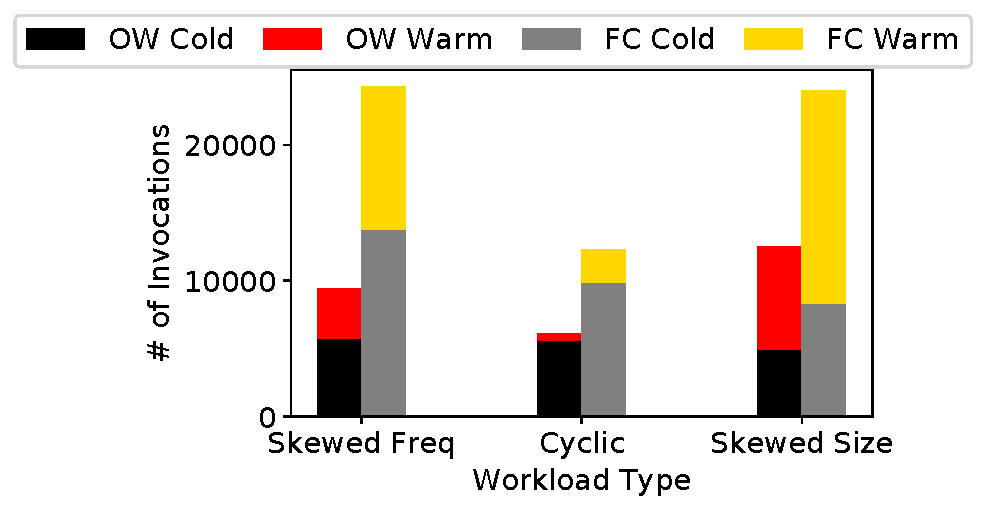
\includegraphics[width=0.6\textwidth]{faascache/faas-keepalive-20/graphs/litmus_tests/litmus_2_stacked.pdf}
  \caption{FaasCache runs 50 to 100\% more cold and warm functions, for skewed workload traces.}
  \label{fig:litmus_2}  
\end{figure}


In this subsection, we evaluate the performance of the FaasCache system on real functions. 
We focus on the performance of FaasCache's Greedy-Dual keep-alive implementation, and compare it to the vanilla OpenWhisk system which uses a 10 minute TTL.


% rev1 1
In contrast to the previous subsection in which we showed the average performance for different cache sizes, we will now also focus on the inverse problem: for a fixed server size, how much more load can be handled with FaasCache? 
By leveraging Greedy-Dual caching, FaasCache is able to reduce cold starts. 
This also reduces the number of \emph{dropped} requests. %

OpenWhisk buffers and eventually drops requests if it cannot fulfill them.
Because FaasCache more effectively selects evictions, its higher hit rate results in functions finishing faster, allowing more functions to be executed in the same time frame.  
%
\begin{table}
  \centering
  \caption{FaaS workloads are highly diverse in their resource requirements and running times. The initialization time can be significant and is the cause of the cold start overheads, and depends on the size of code and data dependencies.}
  \begin{tabular}{lrrr}
    \hline 
    Application & Mem size & Run time & Init. time \\
    \hline
    ML Inference (CNN) & 512 MB & 6.5 s & 4.5 s \\
    Video Encoding & 500 MB & 56 s & 3 s \\
    Matrix Multiply & 256 MB & 2.5 s & 2.2 s \\
    Disk-bench (\texttt{dd})  & 256 MB & 2.2 s & 1.8 s \\
    Image Manip & 300 MB & 9 s & 6 s \\
    Web-serving & 64 MB & 2.4 s & 2 s \\
    Floating Point & 128 MB & 2 s & 1.7 s \\
    \hline
  \end{tabular}
  % \vspace*{\myfigspace}
  \label{tab:fc:workloads}
  %\vspace*{\myfigspace}
\end{table}

To examine the effect of Greedy-Dual keep-alive on cold start and dropped requests, we use a workload trace comprising of four different functions: Disk-bench, ML inference, Web-serving, and Floating-point, described in Table~\ref{tab:fc:workloads}.

In Figure~\ref{fig:litmus_2}, we use different kinds of \emph{skewed} workloads: with a single function having a different frequency, a cyclic access pattern, and a skewed workload with 2 sizes. 
We see that FaasCache's keep-alive can increase the number of warm invocations by between 50 to 100\% compared to OpenWhisk's TTL.
The difference in the total number of requests served (warm+cold) is because OpenWhisk drops a significant number of requests due to its high cold start overhead and resultant system load. 
%
Thus with FaasCache, the total number of requests that are served also increases by $2\times$. 

%rev 1 above 
%Interestingly, OpenWhisk drops a significant number of requests, which is the cause of the different total served requests. 
%

% The impact on the different function performances can be seen in Figure~\ref{fig:faasbench}.
% For this figure, to generate the workload, the first three functions have an inter-arrival time of 1500 ms, and the fourth (floating-point) has a lower IAT of 400 ms. 

%a disk-based one, web-page serving, floating-point trigonomotry operations in numpy, and a convolutional neural network inference (TensorFlow with which model?). % A detailed description of these workloads is required.

% Explain what is the iat distribution and (other details? ).


% 32 GB wted_increase vanilla 11.964% cache 11.528%
% 48 GB wted_increase vanilla 6.184% cache 0.624%


\begin{figure}[t]
  \centering
\includegraphics[width=0.6\textwidth]{faascache/faas-keepalive-20/graphs/litmus_tests/faasbench_48_cold_hot-legend.pdf}
\caption{FaasCache increases warm-starts by more than $2\times$, which also reduces system load and dropped functions.}
\label{fig:faasbench}
\end{figure}


\begin{comment}
\begin{figure}[t]
  \centering
\subfloat[48 GB   \label{fig:faasbench-stacked-48}]
{ \includegraphics[width=0.3\textwidth]{../graphs/litmus_tests/faasbench_48_cold_hot-legend.pdf}}
\hfill 
  \subfloat[32 GB   \label{fig:faasbench-stacked-32}]
{  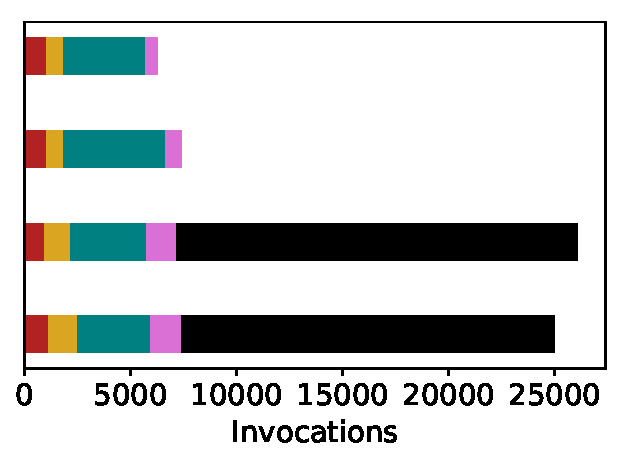
\includegraphics[width=0.17\textwidth]{../graphs/litmus_tests/faasbench_32_cold_hot.pdf}}
\caption{Impact of keep-alive on different function types.}
\label{fig:faasbench}
\end{figure}
\end{comment}

% Figure~\ref{fig:faasbench-stacked-32} shows the number of cold and dropped requests for the different functions, with a medium cache size of 32 GB.
% This setup is intended to evaluate our system in resource constrained environments.
% We see that dropped requests dominate, and FaasCache's more effective keep-alive serves 45\% of requests, while OpenWhisk only serving ~40\%.
% At the same time, warm starts improve 17\% using FaasCache.


Next, we use the skewed frequency workload and use functions from Table~\ref{tab:fc:workloads} to evaluate the impact on real applications. 
%The impact on the different function performances can be seen in Figure~\ref{fig:faasbench}.
To generate the workload, the CNN, DD, and Web-serving functions have an inter-arrival time of 1500 ms, and the Floating-point function has a lower IAT of 400 ms. 
%
Figure~\ref{fig:faasbench} shows the breakdown of different function invocations for this workload on a 48 GB server.
Interestingly, OpenWhisk drops a significant number (50\%) of requests due to the its high cold start overheads.
FaasCache increases the warm requests by more than $2\times$. 
Interestingly, the \emph{distribution} of warm starts is also different. 
FaasCache's Greedy-Dual policy prioritizes functions with higher initialization times, but penalizes those with large memory footprints. 
Because the floating-point function has a high initialization overhead (Table~\ref{tab:fc:workloads}), it sees a $3\times$ increase in hit-ratio compared to OpenWhisk.
\emph{In practical terms, the improvement in keep-alive results in a $6\times$ reduction in the application latency.
}
%The ML inference function has an 8\% lower warm hit rate than the other functions, as it gets de-prioritized because of it's high memory needs.


%When the cache size is increased to 48 GB (Figure~\ref{fig:faasbench-stacked-48}), FaasCache doesn't drop a single request, while OpenWhisk still can't serve 50\% of them.
%For the same workload, Figure~\ref{fig:faasbench-stacked-32} shows the distribution of cold and warm starts for a larger cache size of 32 GB.
%The number of warm starts increases by nearly 20\% compared to OpenWhisk.
% FaasCache's Greedy-Dual policy prioritizes functions with higher initialization times, the CNN function sees a 53\% higher warm starts, wheres Z function only sees X\% increase compared to OpenWhisk. 
% The floating point function has a very high initialization overhead (1.7 of the total 2 seconds), and thus sees its warm-start rate increase the most, by 40\%. 

\begin{comment}
At a smaller cache size of 32 GB shown in Figure~\ref{fig:faasbench-stacked-32}, the number of dropped requests dominate.
This setup is intended to evaluate our system in resource constrained environments.
FaasCache's more effective keep-alive serves 45\% of requests, while OpenWhisk drops nearly 60\%.
Warm-starts increase by 17\% with FaasCache. 
\end{comment}

\noindent \emph{\textbf{Result:} FaasCache can increase the number of warm-starts by $2\times$ to $3\times$ depending on the function initialization overheads and workload skew. This results in lower system load, which increases the number of requests FaasCache can serve by $2\times$.}

%\prat{CPU Graph not required, but just the average numbers will do.}

%%%%%%%%%%%%%%%%%%%%%%%%%%%%%%%%%%%%%%%%%%%%%%%%%%%%%%%%%%%%
\subsection{Effectiveness of Provisioning Policies}
All our previous results have been with a statically allocated server, and 
we now illustrate the effectiveness of our dynamic vertical scaling policy described in Section~\ref{subsec:dynamic}.
The goal is to dynamically adjust the cache size based on the workload. 
Our  policy seeks to keep the miss speed (cold starts per second) close to a pre-specified target. 
This is shown in Figure~\ref{fig:dynamic}---the target is 0.0015 misses per second. 
In this experiment, the cache resizing is done only when the miss speed error exceeds 30\%, and we can see that the cache size increases with the miss speed, and decreases with it. 
Without the dynamic scaling, a conservative provisioning policy would result in a constant, 10,000 MB size. 
In contrast, the average cache size with our proportional controller is less than 7,000 MB.
This 30\% reduction means that FaaS providers can reduce their provisioned resources without compromising on performance.
The freed-up resources can be used to accommodate additional cloud workloads (such as co-located VMs and containers). 
Our dynamic scaling is extremely conservative: increasing its agressiveness by reducing the error tolerance below 30\% will reduce  average server size,
%but cause a larger number of small memory-size  changes, which we wish to avoid.
but we seek to avoid the resultant small changes to memory-size to minimize fragmentation. 
%avoid why?? 

\begin{figure}[t]
  \centering 
  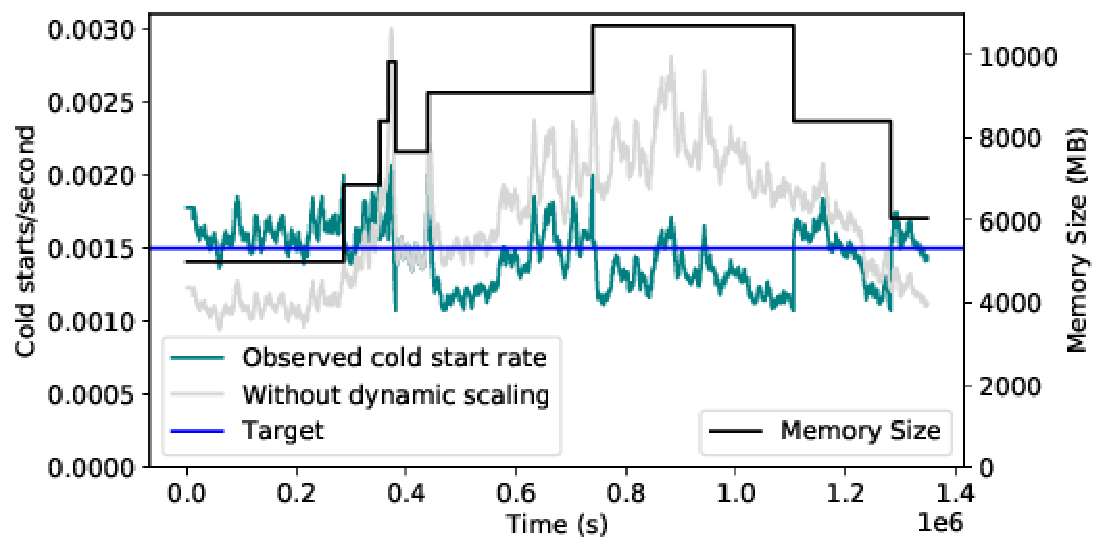
\includegraphics[width=0.6\textwidth]{faascache/faas-keepalive-20/graphs/dyn-scale-392-b.pdf}
  \caption{With dynamic cache size adjustment, the cold starts per second are kept close to the target (horizontal line), which reduces the average server size by 30\%. }
  \label{fig:dynamic}
\end{figure}

%%% Local Variables:
%%% mode: latex
%%% TeX-master: "paper"
%%% End:


\section{Related Works}
\label{sec:faascache-related}

% \section{Related Work}

% \noindent \textbf{Function Keep-alive.}
Mitigating cold starts is one of the central performance problems in FaaS, and has received commensurate attention in both academia and industry.
%
The initialization or startup time of functions can be reduced  by reducing container startup overheads~\cite{oakes_sock_2018,mohan_agile_2019, akkus_sand_2018}, or deploying functions inside ultra-light containers, VMs, or unikernels~\cite{unikernels,firecracker-nsdi20}.
%
While these mechanisms can reduce the cold start overhead associated with the virtual environment creation, other sources of overheads remain, such as losing all application initialized variables, cached files, etc.
As we have shown, keep-alive essentially serves the role of caching, and fast startup only reduces the ``miss'' penalty, and does not eliminate it.

% Rev 1 
Catalyzer~\cite{du2020catalyzer} implements new mechanisms for checkpointing and restoring application and sandbox state, which significantly reduce the initialization cost of functions deployed in their gvisor-based sandbox environment. 
Our approach is complementary to these techniques since we focus on retaining the entire execution environment instead of optimizations for restoring/recreating it. 
Keep-alive policies can be combined with these optimized mechanisms to improve system-wide performance even further. 

%for functions by forking a lightweight execution environment after function initialization. %still uses memory though?
%This reduces duplicate computation, 
%It uses a complementary set of techniques, since we tradeoff extra memory for simpler system and deployment complexity. 

Principled keep-alive policies for functions have recently gained attention: the recent dataset and policy from the Azure function trace~\cite{shahrad_serverless_2020} shows the importance and effectiveness of keep-alive policies. 
In contrast to our work, their policy does not take the function size into consideration and uses a time-series prediction approach (effectively capturing recency and frequency), and combines it with a predictive ``prefetching'' approach. 
As we have shown, function memory footprints are a crucial characteristic, and the use of caching allows the use of advanced analytical and modeling approaches for serverless computing in general. 
% rev 1 
Earlier work has focused on simple ``warm container pools''~\cite{lin_mitigating_2019}, in which Kubernetes cluster runs a certain number of warm containers for functions. 
Our caching-based policies take this one step further and decide \emph{which} container to keep-alive, and for how long. 
Polling to keep cloud functions warm has also been a popular method~\cite{warm2,warm1}.



%
Our work considers functions individually---function scheduling with DAG based approaches~\cite{carver_search_2019} is effective for function-chains, and are orthogonal and complementary to our work. 
%
Hiding function latency using data caching (such as redis) for database applications is investigated in~\cite{ghosh_caching_2019}. 
The ENSURE~\cite{ensure_acsos20} system handles keep-alive and resource provisioning for CPU resources using queuing theory techniques.
Our focus is on memory-constrained keep-alive and provisioning, and CPU-focused approaches are complementary to our work. 

\subsection{Comparative Works}

FaasCache has inspired a number of new caching policies, and of everything in this thesis has become the most popular system to reference and compare against.
Listed here are those that directly compare against FaasCache.
Heterogeneous FaaS workers~\cite{roy2022icebreaker} and predictive prewarming of containers~\cite{saha2024fase} can improve performance.
Edge computing has strict resource requirements, and uses a mix of scheduling and cache management to minimize cold starts~\cite{zhang2023online,chen2024cross}.
Invocations can also be intelligently scheduled, batched, and re-ordered to avoid cold starts~\cite{wu2024faasbatch,cai2024incendio}.

\begin{comment}
\noindent \textbf{Caching.}
Our choice of Greedy-Dual-Size-Frequency was motivated by the ease with which its parameters mapped to function keep-alive, in particular the frequency vs. size tradeoff.
Cache eviction algorithms have a long history, although the focus has predominantly on uniform sized objects (such as disk blocks, RAM pages, cache lines, etc.).
Certain caching optimizations relying on spatial locality (such as look-ahead and ARC) are not directly applicable to keep-alive. 
The size-aware cache algorithms and models used for web-caches, proxies, and CDNs form the basis of our work. 
Cache provisioning using hit/miss ratio curves is a common approach, and these curves can also be constructed dynamically, which is part of our future work.
%
\end{comment}

\begin{comment}

The Azure function traces and keep-alive approach 

Prior work has investigated reducing container startup overheads, which can reduce the 

\noindent \textbf{Usecases}

~\cite{cartas_reality_2019} questions the need for edge computing for ML inference, because of the decreasing inference latency and costs, and network latency becomes the primary bottleneck.

Berkeley view~\cite{jonas2017occupy, jonas_cloud_2019}

Interactive applications---RunBox ~\cite{glikson_runbox_2019}.

Data analytics with ServerMix~\cite{garcia-lopez_servermix_2019}

ExCamera

PyWren

Serverless analytics with Flint wtf

From laptop to lambda ~\cite{fouladi_laptop_2019}

Monolithic to serverless with Ripple~\cite{joyner_ripple_2020}

HPC~\cite{mocskos_faaster_2018}

SPEC group report~\cite{van_eyk_spec_2017}

\noindent \textbf{cold start problem}

~\cite{lin_mitigating_2019} is a project report that uses ML inference, webserver workloads as we are. Knative platform. Maintain a pool of warm containers. No real policy though.

HyperFaas claims to address cold start problem? ~\cite{zhang_hyperfaas_2019}. 

\noindent \textbf{Keep-alive Mechanisms.} Most closely related work goes here.. 

\noindent \textbf{Frameworks}

Cirrus~\cite{carreira_cirrus_2019} does end to end ML model training, hyperparam tuning on a new serveless framework. Not inference though?

SAND~\cite{akkus_sand_2018} is based on openwhisk, but focused more on the inter function messaging?

Wukong~\cite{carver_search_2019} has an interesting DAG scheduling solution---decentralized scheduling. Evalutes on numerical computing problems and compares with Dask (Python).

SPOCK~\cite{gunasekaran_spock_2019} combines VMs and serverless functions. 

Named functions as a service~\cite{krol_nfaas_2017}---uses unikernels!!
More work along similar lines~\cite{lin_computation_2019,mtibaa_towards_2018,xylomenos_named_2019,krol_computation_2018}


Peeking behind the curtains

SOCK~\cite{oakes_sock_2018}

OpenLambda~\cite{hendrickson2016serverless}

GrandSlam ~\cite{kannan_grandslam_2019} ~\cite{} tries to provide SLA guarantees for microservices.

Performance comparison by Geoffrey~\cite{lee_evalution_2018}


\noindent \textbf{Resource management}

Auction based function placement in serverless~\cite{bermbach_towards_2019}.

Checkpointing and migration with CRIU for IoT devices in~\cite{karhula_checkpointing_2019}. What's the motivation with stateless functions? Nothing---they focus on stateful functions.


``Living on the edge''~\cite{kulkarni_living_2019} explores transaction support and fault tolerance for stream processing. 


Data management (really caching?) with the Locus shuffling system~\cite{pu_shuffling_2019}. 


Caching strategies for data in~\cite{ghosh_caching_2019}

More storage optimizations?~\cite{zhang_narrowing_2019}

\noindent \textbf{Formal }

~\cite{hall_execution_2019} provides an architecture with WASM on the edge.

~\cite{riis_nielson_no_2019} provides a serverless kernel calculus combining lambda calculus for computation and pi-calculus for communication.

\end{comment}



%%% Local Variables:
%%% mode: latex
%%% TeX-master: "paper"
%%% End:


\begin{comment}
\cite{faascache-asplos21}

Platforms today exhibit eager eviction, always trying to have memory available to facilitate possible cold starts.
My work called FaasCache~\cite{faascache-asplos21}, reinterprets this paradigm.
We can choose instead to keep all sandboxes around indefinitely and only remove them when we must make room for an invocation we do not yet have a sandbox for.
It casts the eviction choice as a caching decision, where better eviction decisions lead to more cache hits (warm starts for invocations).
Taking into account a function's memory allocation, how often it is invoked, its recency, and the cost of having to re-initialize it, we can make more optimal decisions on what to keep.
Thereby giving a much higher warm hit ratio.
\end{comment}

\chapter{Load- and Locality-Aware Load Balancing}
\label{chap:chrlu}

% While serverless computing provides more convenient abstractions for developing and deploying applications, the Function-as-a-Service (FaaS) programming model presents new resource management challenges for the FaaS provider. 
In this chapter, we investigate load-balancing policies for serverless clusters and find that the locality vs. load tradeoff is crucial and presents a large design space.
Locality, i.e., running repeated invocations of a function on the same server, is a key determinant of performance because it increases warm-starts and reduces cold-start overheads. 
% We find that the locality vs. load tradeoff is crucial and presents a large design space. 

We enhance consistent hashing for FaaS, and develop CH-RLU: Consistent Hashing with Random Load Updates, a simple practical load-balancing policy which provides more than $2\times$ reduction in function latency. 
Our policy deals with highly heterogeneous, skewed, and bursty function workloads, and is a drop-in replacement for OpenWhisk's existing load-balancer.
We leverage techniques from caching such as SHARDS for popularity detection, and develop a new approach that places functions based on a tradeoff between locality, load, and randomness. 


\section{Related Work}

\subsection{Load Balancing Related Work}

\begin{comment}
\noindent \textbf{FaaS Resource Management.}
The initialization overheads of serverless functions and their repeated invocations have spawned a great deal of research into optimizing their resource management.
Recent surveys~\cite{faas-survey-jan-2022, raza2021sok, eismann2020serverless, hassan2021survey, mampage2021holistic} provide an overview of the challenges and solutions in this very active research area. 

Reducing the overhead of serverless functions through various systems and virtualization-level mechanisms and  optimizations~\cite{du2020catalyzer, firecracker-nsdi20, dukic2020photons, akkus_sand_2018, vhive-asplos21, carreira2021warm}. 
%
Locality for FaaS resource management has been explored in the form of function keep-alive policies~\cite{shahrad_serverless_2020}. 
Our work builds on and uses the caching-based Greedy-Dual policy from FaasCache~\cite{faascache-asplos21}. 
%
Single-server environments have been the focus of these mechanisms and policies: we have made an initial attempt to understand their interactions in a distributed cluster context.
%
Inter-function dependencies can also be used for predictive resource management and reducing function communication and startup costs~\cite{gunasekaran2020fifer, daw2021speedo, shen2021defuse}: incorporating these policies into our load-balancer is part of future work. 
\end{comment}

% \noindent \textbf{Function Load Balancing:}
Package-aware load balancing~\cite{package-cristina-19}  identifies and uses function code dependencies (software packages) as an important source of data locality.
While this is an important factor, we focus on in-memory locality of kept-alive functions, since memory capacity is much smaller than permanent storage and caching functions in memory has a very large performance impact.
%
CPU contention and interference is a major source of performance bottlenecks for co-located functions, and adjusting CPU-shares using cgroups can provide significant benefits~\cite{suresh2019fnsched, suresh2021servermore, ensure-faas-acsos20}.
%
The load-locality tradeoff we explore is complementary to these CPU scheduling optimizations. 
%
The repetitive nature of functions and their workflows can also be used to improve resource utilization and latency~\cite{hunhoff2020proactive, yu2021faasrank, puru_xanadu_20, przybylski2021data}: our load-balancer is stateless for the sake of simplicity and can be enhanced with these techniques if necessary.


The tradeoff between locality and performance has also been explored in the context of delay scheduling~\cite{zaharia2010delay} for data-parallel applications like MapReduce.
Load-balancing is seen as a ``dispatch'' problem in queuing theory, and the FaaS cluster system most closely approximates G/G/PS, since the arrivals and service times are not markovian.
Techniques such as ``join the shortest queue'', and ``least work left''~\cite{gupta2007analysis} have been shown to be effective.
The online-greedy policy evaluated in the previous section closely approximates least-work-left.
However, it is difficult to implement in practice since the running times of functions is hard to predict due to their volatile arrival distribution mixtures and high variances in running time due to various system interference effects.



% In general, 
% CH, dynamo,
% CH-RJ not applicable because of lack of locality.
% Stale loads dahlin, mitzen,
% power of 2 choices: but not locality aware and load has an uncertain bearing on performance.
% \subsection{Queuing and Dispatch}
% Remaining time times the original size (RS) ~\cite{scully2022bounding}
% Guardrails:~\cite{}
% Although we focus on the heavy-traffic regime with server loads far exceeding one. 

%%% Local Variables:
%%% mode: latex
%%% TeX-master: "paper"
%%% End:


\subsection{QoS Related Work}

% \noindent\textbf{FaaS Resource Management:}
% Multiple recent projects have looked into ways for optimizing the resource management of serverless frameworks, including solutions that
% reduce the overhead of the cloud functions~\cite{du2020catalyzer, firecracker-nsdi20, dukic2020photons, akkus_sand_2018, vhive-asplos21, carreira2021warm},
% improve locality through keep-alive policies~\cite{Shahrad:ATC:2020:ServerlessInTheWild},
% better caching algorithms for worker nodes~\cite{faascache-asplos21},
% reducing function communication and startup costs~\cite{gunasekaran2020fifer, daw2021speedo, shen2021defuse}, among others. 
% Our work leverages the caching-based Greedy-Dual policy~\cite{faascache-asplos21}, in a cluster with pools that support differentiated services for high- versuls low-priority functions.

% \noindent\textbf{Latency-sensitive scheduling and load balancing in serverless:}
% Nightcore~\cite{jia2021nightcore} provides low end-to-end latency and variability using fast paths for internal calls, low-latency message channels, efficient threading and concurrency.
% Atoll~\cite{singhvi2021atoll} uses deadline-aware two-level scheduling as part of a low-latency serverless platform.
% Our proposal can be added to those solutions to further implement differentiated services on top of more performant serverless platforms.
% In general, there is a rich previous body of work in performance improvement methods~\cite{soakes_sock_2018,kaffes2019centralized,hunhoff2020proactive} that are complementary to our approach.
% In addition, we extend the notion of locality-aware function routing~\cite{firecracker-nsdi20,aumala2019beyond,abdi2023palette} and use it within cluster pools that ensure differentiated services when functions can be divided into priority classes. 

\mhead{Differentiated services in serverless}
Sequoia~\cite{Tariq:SOCC:2020:Sequoia} is a serverless framework with a QoS scheduler based on a simple priority-based queue; however, the issue of starvation in the presence of a continuous arrival of high-priority functions is not considered.
Furthermore, the framework is based on a completely new design that does not support synchronous function calls.
In contrast, our solution was implemented on top of OpenWhisk and considers both synchronous and asynchronous functions.
Bilal et al.~\cite{Bilal:CoRR:2021:GreatFreedom} analyzed the trade-off space between performance and cost that arises from different CPU/RAM configurations and the resulting function performance.
This approach is orthogonal to ours and can be leveraged by the provider to offer differentiated services that span this configuration space.
Qiu et al.~\cite{Qiu:WOSC:2021:LatencyCritical} suggested that providers could implement resource over-commitment for FaaS workloads with loose latency objectives;
our approach ties over-commitment with current demand, with a dynamic mechanism that supports handling of bursts in high priority workloads at the expense of low priority ones.
\emph{Real-time serverless}~\cite{Nguyen:WoSC:2019:Real-Time} is a work-in-progress system that describes an interface for specifying invocation rate guarantees and proposes delivering them via admission control and predictive container management.

% \noindent\textbf{Workload shifting in the cloud:}
% Delaying of tasks has been proposed to make better use of renewable excess energy~\cite{Wiesner:Middleware:2021:TemporalShifting,Wiesner:EuroPar:2022:Cucumber}, to reduce
% energy consumption for workflow execution~\cite{Versluis:HotCloudPerf:2022:TaskFlow}, among others.
% While we have not implemented policies with energy management goals, our solution could be extended to consider energy information (peaks, variable costs, green energy availability).

\mhead{Multi-pool cluster scheduling}
Virtual cluster pools have been used for dynamic resource management in datacenters~\cite{Chase:HPDC:2003:COD}, to handle increased workloads in data analytics clusters~\cite{Lee:HotCloud:2011:Heterogeneity-Aware}, for QoS multi-class admission control~\cite{Delimitrou:ICAC:2013:ARQ}, and to decrease the delays of scheduling decisions~\cite{singhvi2021atoll}. 
We use this technique for service differentiation, and complement it with a novel control-based dynamic resizing mechanism to support burst absorption in serverless workloads.
%Note: {Lee:HotCloud:2011:Heterogeneity-Aware} uses too pools: core nodes and accelerator nodes; the latter are temporarily added to the cluster to handle increased jobs (observed or anticipated).

\mhead{Current Status of Differentiated FaaS Invocations}
\label{sec:motivation:currentStatus}
A recent empirical study~\cite{Tariq:SOCC:2020:Sequoia} found that current cloud providers (AWS, Azure, GCP and IBM) treat HTTP functions differently from those triggered by other means, frequently via undocumented behavior, including different concurrency limits and prioritization versus background functions.
In addition, while asynchronous functions are queued and thus the user understands that they may not execute immediately, providers don't typically enqueue synchronous functions but rather return with an error if peak exceeds concurrency limits or provider capacity.\footnote{An exception is GCP which handles synchronous calls in best effort fashion, performing queuing but not ensuring zero drops~\cite{Tariq:SOCC:2020:Sequoia}.}
%
Thus, the major public cloud providers are already implicitly defining two classes of functions: high priority (synchronous) and lower priority (asynchronous), with the latter being delay-tolerant.
%asynchronous functions in AWS can be queued up to 6 hours.\footnote{\url{HTTPs://docs.aws.amazon.com/lambda/latest/dg/invocation-async.html}}
%Asynchronous functions are either explicitly (for example, with the \texttt{async} keyword in OpenWhisk) or implicitly (by its trigger) defined in current platforms.
%The asynchronous functions are good candidates to be delayed if needed.

In OpenWhisk asynchronous functions are defined with the \texttt{async} keyword and follow a different execution path than synchronous ones.
However, the platform does not use any mechanism to delay or execute them at a lower priority.
A solution that treats \texttt{async} functions as delay-tolerant, scheduled with a lower priority than synchronous functions, can be added to OpenWhisk without API modifications.

%
% OLD, conference-paper related work
%
% \noindent \textbf{FaaS Resource Management.}
% The initialization overheads of serverless functions and their repeated invocations have spawned a great deal of research into optimizing their resource management.
% Recent surveys~\cite{faas-survey-jan-2022, raza2021sok, eismann2020serverless, hassan2021survey, mampage2021holistic} provide an overview of the challenges and solutions in this very active research area. 

% Reducing the overhead of serverless functions through various systems and virtualization-level mechanisms and  optimizations~\cite{du2020catalyzer, firecracker-nsdi20, dukic2020photons, akkus_sand_2018, vhive-asplos21, carreira2021warm}. 
% %
% Locality for FaaS resource management has been explored in the form of function keep-alive policies~\cite{shahrad_serverless_2020}. 
% Our work builds on and uses the caching-based Greedy-Dual policy from FaasCache~\cite{faascache-asplos21}. 
% %
% Single-server environments have been the focus of these mechanisms and policies: we have made an initial attempt to understand their interactions in a distributed cluster context.
% %
% Inter-function dependencies can also be used for predictive resource management and reducing function communication and startup costs~\cite{gunasekaran2020fifer, daw2021speedo, shen2021defuse}: incorporating these policies into our load-balancer is part of future work. 

% \noindent \textbf{Function Load Balancing:}
% Package-aware load balancing~\cite{package-cristina-19}  identifies and uses function code dependencies (software packages) as an important source of data locality.
% While this is an important factor, we focus on in-memory locality of kept-alive functions, since memory capacity is much smaller than permanent storage and caching functions in memory has a very large performance impact.
% %
% CPU contention and interference is a major source of performance bottlenecks for co-located functions, and adjusting CPU-shares using cgroups can provide significant benefits~\cite{suresh2019fnsched, suresh2021servermore, ensure-faas-acsos20}.
% %
% The load-locality tradeoff we explore is complementary to these CPU scheduling optimizations. 
% %
% The repetitive nature of functions and their workflows can also be used to improve resource utilization and latency~\cite{hunhoff2020proactive, yu2021faasrank, puru_xanadu_20, przybylski2021data}: our load-balancer is stateless for the sake of simplicity and can be enhanced with these techniques if necessary.


% The tradeoff between locality and performance has also been explored in the context of delay scheduling~\cite{zaharia2010delay} for data-parallel applications like MapReduce.
% Load-balancing is seen as a ``dispatch'' problem in queueing theory, and the FaaS cluster system most closely approximates G/G/PS, since the arrivals and service times are not markovian.
% Techniques such as ``join the shortest queue'', and ``least work left''~\cite{gupta2007analysis} have been shown to be effective.
% The online-greedy policy evaluated in the previous section closely approximates least-work-left.
% However, it is difficult to implement in practice since the running times of functions is hard to predict due to their volatile arrival distribution mixtures and high variances in running time due to various system interference effects.


%%% Local Variables:
%%% mode: latex
%%% TeX-master: "paper"
%%% End:



\section{Background: Load Balancing}

Managing the load of a cluster of servers is a common problem in distributed computing systems.
Load-balancing policies typically rely on some notion of ``load'' of a server, such as the number of concurrently executing tasks, length of the task-queue, cpu-utilization, etc.
%
The first broad class is \emph{compute-oriented} load-balancers, typically used for short-running tasks and queries. 
Load-balancing for computational tasks is common in scenarios like web-clusters~\cite{karger1999web}. 
In these systems, the tasks can be executed on any server,  servers in a cluster are largely fungible, and the task performance largely depends on the server-specific cpu-utilization at the time.

Load-balancing techniques have received significant theoretical attention (especially using queuing theory), as well as many practical systems~\cite{decandia2007dynamo}. 
From a queuing theory perspective, policies such as least-work-left (LWL) and Join-Shortest-Queue (JSQ), have studied near-optimal load balancing for computing load-dependent workloads under a processor-sharing (PS) setting. 

Interestingly, load-balancing for \emph{data-oriented} systems, such as Content Delivery Networks (CDNs)~\cite{nygren2010akamai}, and distributed key-value stores (such as Amazon Dynamo~\cite{decandia2007dynamo}) must also balance the load on servers, but with data locality as a key requirement.
In this context, locality refers to requests for the same object being handled by the server, or the same subset of servers if the object is replicated. 
We find that FaaS load balancing requires and benefits from \emph{both} these objectives: minimizing computing load \emph{and} maximizing locality to reduce cold starts. 

\begin{comment}
However, combining compute-oriented load-balancing solutions 

In large clusters, consistent load information cannot always be assumed, and simple techniques work well in practice.
For instance, the power of two random choices, which schedules a task on the least loaded of two random servers. 

Queuing analysis?
- G/G/PS system. Greedy load balancing is sub-optimal.

Randomization and power of 2 choices is popular.

But arent locality aware.

Web server load balancing work. A Gandhi etc. 
\end{comment}

%\vspace*{-0.2cm}
\subsection{Consistent Hashing} 
\label{subsec:ch}

\begin{figure}
  \centering
  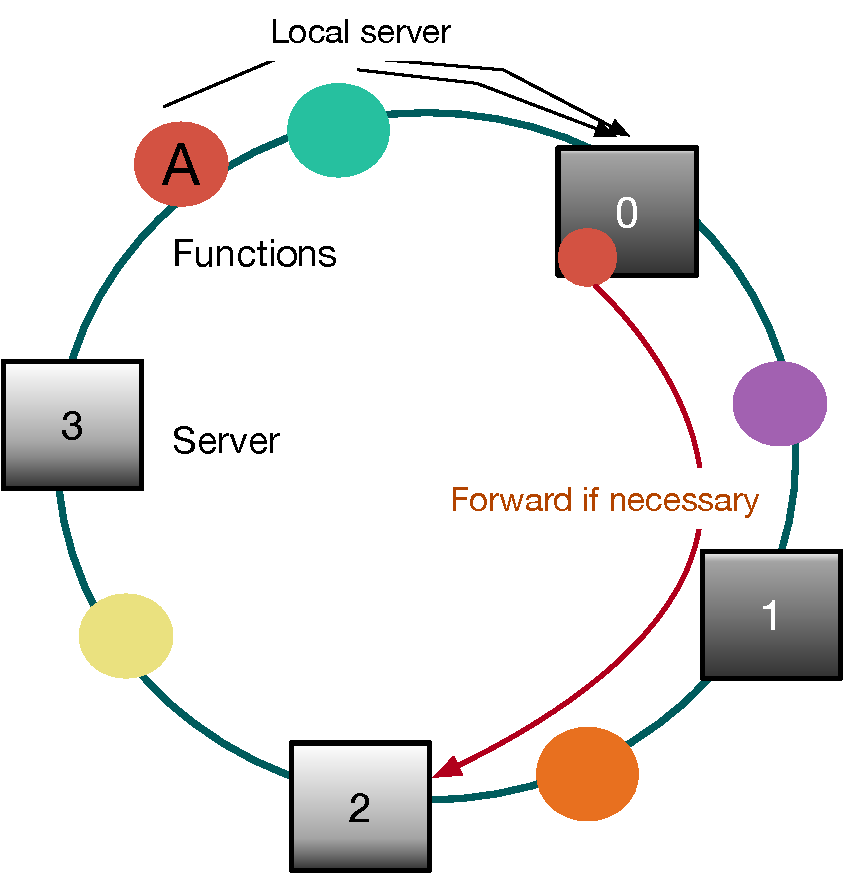
\includegraphics[width=0.7\textwidth]{chrlu/faaslb-osdi22/figs/ch-bl.pdf}
%  \vspace*{-0.2cm}
  \caption{Consistent hashing runs functions on the nearest clockwise server. Functions are forwarded along the ring if the server is overloaded.}
  \label{fig:ch}
%    \vspace*{-0.2cm}
\end{figure}

For data-oriented systems, a common technique to ensure locality is Consistent Hashing~\cite{karger1999web, karger1997consistent}.
Objects are mapped to servers based on some object id or key.
Consistent hashing preserves object-server mapping even in the face of server additions and removals, which improves locality.
%
Figure~\ref{fig:ch} provides an overview of consistent hashing. Both objects and servers are hashed to points on a ``ring'', and objects are assigned to the next server (in the clockwise direction) in the ring. 
Addition or removal of servers only affects the nearby objects by remapping them to the new next server in the ring.

OpenWhisk uses a modified consistent hashing algorithm for its default load balancer.
As functions are sent to servers, their expected memory footprint is added to a server-specific running counter of outstanding requests.
Upon completion the memory size of a function is decremented from that server's counter.
If the counter for a function's \quotes{home} server would exceed the assigned memory on the server it is forwarded along the ring.
%
The drawback of this policy, and consistent hashing as a whole, is that the performance can be affected by the relative popularities of the different objects.
A highly popular object can result in its associated server getting overloaded.
This problem is exacerbated in the case of FaaS functions, as we shall demonstrate in the next section. 


\section{Load-aware Consistent-Hashing} % Based Load Balancing Policies}
\label{sec:chrlu}

In this section, we describe the load-balancing algorithm which is locality, stale-load, and burst aware.
We assume a cluster  homogeneous servers, and 
a new function invocation can be sent to any of the servers.
Each server implements keep-alive for functions: after successful execution, the function's container is stored in server memory, and evicted based on some eviction policy. % such as LRU, TTL, or Greedy-Dual~\cite{faascache-asplos21}. 
%Subsequent invocations of the function constitute  a ``warm'' start which is significantly faster than a cold start. 
%The keep-alive policy determines when and which functions to evict when the server memory is fully occupied by running and ``warm'' containers.

% Thus, locality is crucial for achieving low latency.
% Data storage clusters such as distributed key-value stores also require object-access requests to be routed to the same set of servers.
% However, locality is a stronger constraint in data storage because of consistency requirements. 
% In the case of functions, locality is preferable, and server loads are also considered. 

% Where is the queuing theory perspective? LWL/ SJF/ dispatch. Highly variable job lengths.
%\vspace*{-0.2cm}
\subsection{Tradeoff between Locality and Load}

We use consistent hashing as the fundamental principle to ensure high locality: repeated invocations of the same function occur on the same server. 
However, popular functions, i.e., which are invoked very frequently, can result in overloaded servers.
Because function performance is affected by server load and resource availability, focusing on locality alone can result in slow function execution.

Function popularities are also highly skewed: a small percentage account for a vast majority of invocations.
With pure locality-based load-balancing, the servers of these popular functions would be severely overloaded.
Functions also can run for significantly longer than simple web requests, and thus they impose more load on servers, and the cost of a wrong placement decision is higher. 
This, combined with bursty invocations, can significantly increase the tail latency of functions. 
Thus pure-locality policies such as classical consistent hashing are not sufficient, and 
our research question is: \emph{Can consistent hashing be used to reduce latency due to overloaded servers?} 
Or put another way, can we balance the tradeoff between function locality and server-loads with consistent hashing? 


Our key idea is to extend consistent hashing to take also into account server loads, the cold start overheads of different functions, and the bursty traffic that is a key characteristic of FaaS workloads.
In the rest of this section, we describe our approach. 

% \subsection{Broad design Criteria}
% LB latency is important: millisecond pricing, so LB cant take up too many cycles.

%\vspace*{-0.2cm}
\subsection{Key Principle: Load-based Forwarding}

To balance the locality vs. server load tradeoff, we build on a new variant of consistent hashing called Consistent Hashing with Bounded Loads~\cite{mirrokni2018consistent} (abbreviated as CH-BL in the rest of the chapter).  
The key idea behind CH-BL is to use consistent hashing to locate servers for objects, and if the servers are ``full'', then ``forward'' the objects to the next server in the consistent hashing ring.

For example, in Figure~\ref{fig:ch}, function A is originally assigned to server 0, but this ``home'' server is overloaded (already running many functions), and thus the function is forwarded along the ring until a suitable non-overloaded server (2) is found. 
Any 5-independent hashing function can be used for determining the ``home'' server of a function. %which is determined by hashing the function's unique id. 
Users can specify the load upperbound or the capacity of the server ($b$), which determines the max load the server can sustain.  
Consistent hashing with bounded loads provides many strong theoretical guarantees on the length of the forwarding chain until the object is safely placed on a server. 


Interestingly, forwarding along the ring not only avoids server overloads, but also improves locality, \emph{even in overload scenarios.}
Forwarding along the ring has the advantage that even if function is not run on its ``home'' server, subsequent invocations that ``overflow'' still have a high warm-start probability on the servers on the overflow chain. %, with the warm-start probability decreasing in chain-length.
The warm-start probability is highest on the home server, and decays the farther the function is from its home server. 
This is more beneficial than alternative techniques such as Consistent Hashing with Random Jumps~\cite{chrj-aaai21}, which do not preserve locality and instead forwards to randomly chosen least loaded servers. 

%\vspace*{-0.2cm}
\subsection{Server Load Information}

Server load is a key metric in load-balancing policies.
We need to be able to determine the \emph{relative} suitability of one server over another, and thus many existing metrics can be used to provide information about server loads.
%
Simple metrics such as number of running functions are insufficient, since functions can have highly variable execution times. 
OpenWhisk currently uses occupied-memory used by active/running invocations as a proxy for load, and is unsuitable for the same reason. 
Both these metrics fail to capture CPU loads and lead to scalability issues when used by the load-balancer. 


% OpenWhisk currently uses occupied-memory as a proxy for load.
% However both these approaches require the load-balancer to keep accurately track of which function invocations and \emph{completions} on each server, which creates a scalability bottleneck.
% Furthermore, using memory availability is not suitable for resource-conserving keep-alive policies such as LRU or Greedy-Dual, which have been shown to be much more effective than OpenWhisk's default Time-to-Live (TTL) based eviction.


Instead, we primarily rely on \emph{system-level} load metrics, such as the standard Linux 1-minute load-average.
In addition to CPU utilization, this also captures the I/O wait due to cold starts, and provides a more realistic measure of load.
Traditional Linux load-average estimates the total number of processes running and ready-to-run, and we normalize the load-average by the number of CPUs. 
Thus, a load-average of $8$ on an 8 core server (discounting hyperthreading) is normalized to 1. 

An important practical consideration is that load information is often \emph{stale}, with the degree of staleness ranging from a few seconds to several minutes. 
For instance, because the Linux load average is an exponential moving average, it is slow to change.
Furthermore, load monitoring and reporting has delays due to how frequently the metrics are gathered at the local server, and how often they are made available to the load-balancer.
We use a simple publish-subscribe-like system, where individual servers periodically (every 5 seconds) push their load information, and the load-balancer uses these published loads to make all scheduling decisions.


%\subsection{Cold start Aware Bounded-Loads

%\vspace*{-0.2cm} % Challenges of CH-BL adoption. 
\subsection{Why CH-BL Is Insufficient}

The high computing load of functions, their bursty nature, and the staleness of loads, are the three major challenges to Consistent Hashing with Bounded Loads~\cite{mirrokni2018consistent} that the original algorithm is not designed to meet. 
There are a few practical considerations and key differences between simple object/storage caching and function execution:
1. CH-BL does not take into account the heterogeneity in running times and memory size of the objects (i.e., functions).
2. The implicit CH-BL performance model is binary: running-time is assumed to be uniform as long as servers are under the load-bound. 
3. The server loads evolve as a result of the actual function execution and are not just uniformly incremented as in the original algorithm. Object deletions are also not handled explicitly: we let the lazily computed load average determine whether a server meets the load-bound or not. 

\emph{Importantly, we do not assume complete and consistent state information about the servers.}
Omniscient knowledge of the execution state of all functions running all servers can certainly be leveraged effectively to run functions on the most suitable server.
However, such maintaining such global knowledge is expensive and impractical as far as storage consistency and latency are concerned.
Thus, we are striving for load-balancing policies which are robust to stale, incomplete, and coarse-grained information about server states. 
In the rest of this section, we shall show how the above three limitations of CH-BL can be overcome in FaaS load-balancing settings. 

%\vspace*{-0.4cm}
\subsection{Incorporating Function Performance Characteristics}
\label{subsec:chch}


Different running time and performance characteristics of functions can be incorporated into consistent hashing.
\emph{The key problem is to determine when and which function to forward.}
The forwarding policies need to be cognizant of the warm and cold running times, and the sensitivity to load of different functions. 

%Each server has a load-bound which we do not want the server's load to exceed. As described in the previously, consistent hashing with bounded loads can ensure that no individual server exceeds the load-bound $c$, by forwarding the request (in our case, function invocation) to the next server in the ring, until a suitable server is found. This bound determines what the maximum load of the servers will be. 


Assume a load-bound of $b$, the warm time of a function is $w$, and the cold time is $c$ (slow-start). 
%
The current or the home server will be ``0'', and the next server in the ring that the function may be forwarded-to will be denoted by ``1''. 
Running it on the ``home''/local server will result in expected time $E[T_0] = (p_0w+(1-p_0c)S(L_0) $, where $p_0$ is the cache-hit/keep-alive probability, and $S(L_0)$ is the slowdown in function if the load on the server is $L_0$. 
When a function in invoked the load balancer has the choice to either run in on the home server or forward it to the next server, where it is less likely to be found in the keep-alive cache, because the reuse-distance is much larger for the servers down the chain.
Therefore we can compute the forwarding regret, $E[T_0]/E[T_1]$.

The properties of bounded-loads allows us to easily compute this value.
The probability of being forwarded is small, and is $1/b$ based on Lemma 4 of~\cite{mirrokni2018consistent}.
The reuse-distance of the function, and hence the hit-rate on the original/home server will be larger: $p_0 > p_1*b$. 
% Based on our empirical observation of sub-linear performance decrease due to load (Section~\ref{subsec:function-perf}), in the worst case, the home server will be overloaded and alternative server will not be, and hence the ratio of slowdowns, $S(L_0)/S(L_1) > b$.
Based on our empirical observation of sub-linear performance decrease due to load (elided for space), in the worst case, the home server will be overloaded and alternative server will not be, and hence the ratio of slowdowns, $S(L_0)/S(L_1) > b$.
%
Minimizing the regret, we get that the function should be forwarded if $L>cb/w$.
Thus, the effective load upper-bound is \emph{increased} by a factor of $\text{cold}/\text{warm}$  time, allowing us to run more functions per server. 
In our empirical evaluation, we will show that this can significantly improve performance over plain CH-BL with a function-agnostic constant load-bound.
If the cold and warm times of a function are not available, then they are assumed to be equal, thus this degrades to classic function-agnostic bounded-loads. 


%%%%%%%%%%%%%%%%%%%%%%%%%%%%%%%%%%%%%%%%%%%%%%%%%%%%%%%%%%%%

%\vspace*{-0.4cm}
\subsection{Handling Bursts}
\label{subsec:bursty}

Functions come in a variety of frequency classes and are also prone to unpredictable burstiness (i.e., very low inter-arrival-times for a short duration). 
Identifying these bursts and both keeping latency for such \quotes{popular} functions low and preventing them from negatively impacting co-located functions is critical.
We have found that handling overload conditions is a key requirement and can significantly affect the tail latency.

Bursty function invocations result in two main problems.
First, they cause an increase in server load beyond the actual load-bound, because load is only lazily tracked.
The delayed load information can result in a popular function completely overwhelming a server, causing load \quotes{hotspots} in the cluster.
The second problem is that in extreme cases, the inter-arrival-time is less than the function latency, causing concurrent invocations.
Even if these concurrent invocations are run on a \quotes{local} server with the function present in the keep-alive cache, there will still be cold starts, since each invocation must run in its own container. 

Our solution to these two problems caused by bursty invocations is to detect popular function bursts, ``spread'' these invocations around multiple servers to prevent cluster hot-spots, and use stochastic/random load updates to introduce randomness into the load-balancing. 

\begin{comment}
Multiple problems. 1. Increase the load beyond the bound because lazily tracked. 2. Concurrent: no warm starts. Spreading them around will be useful. 

The problem of concurrent invocations is vexing even with locality, since containers may be in use and thus results in cold starts for these invocations. In the worst case we must accept $n-1$ cold starts for an $n$ core server. 

% Very popular functions can present problems.
We use two strategies:
1. Identify popular functions in a low-overhead online manner.
1a. Use this information to inform the load estimate. Due to the problem of \textbf{stale loads.}
2. Extreme overload: pick least loaded server if going around the horn.  % this seems orthogonal. 

This is similar to epsilon-greedy: we greedily pick the server based on the expected running time estimate for unpopular functions and probabilistically for popular functions. 
The probability is determined based on the server load and the noise in the server load estimate, which in turn depends on the estimate of the recent arrival rate of the functions. 

\end{comment}

%\vspace*{-0.2cm}
\subsubsection{Detecting Popular Functions with Spatial Sampling}

Our goal is to detect ``popular'' functions with low inter-arrival-times, in an online low-overhead manner.
%
Popularity detection must take into account the changing invocation frequencies of different functions over time, and be low-overhead.
We identify the top \textit{p} percentile of functions by their inter-arrival-times (IAT), or below some explicit IAT threshold, to reduce unnecessary hyperparamaters. 

Our approach is general: we first build a histogram of inter-arrival-times using sampling, and then query it. 
We note similarities with computing reuse-distance histograms, which are the building block of miss-ratio curves. 
%Our goal is to find the popular functions that have a low inter-arrival-time (IAT) quickly.
Reuse-time histograms are a simpler version of reuse-distances.
Recall that reuse distance is the number of \emph{unique} objects accessed, whereas inter-arrival-time is simply the difference in wall-clock times.
%In particular, we use the SHARDS technique, and modify and simplify it to compute an approximate IAT distribution instead of a reuse distance distribution. 



Our solution to identifying popular functions and function bursts is inspired by the popular SHARDS~\cite{shards} algorithm for building reuse-distance histograms. 
%
Following SHARDS, we randomly sample invocations to track individual function IATs. 
This tracking is simplified by only recording the most recent access time, and then computing the IAT as an estimated moving average of the current IAT and  $now - last\_access$. 
These values are tracked for every function, and functions in the top $p^{th}$ percentile of IATs are considered \textbf{popular}.
%
For the sampled functions using spatial hashing, we update their IAT.
Note that this approach keeps only a small number of last-accessed-iat entries in memory: ``have-been'' popular functions are naturally evicted from the tracking list. 
Because we do not care about reuse-distances, we avoid keeping a tree of reuse-distances, resulting in a simplified SHARDS-like algorithm (see Algorithm~\ref{algo:shards-popular}). 


% \begin{lstlisting}
% def update_shards_popular(func, time):

% if Ti < T:
%   if func in last_access_times:
%     # Already in our sample set 
%     iat = (t-last_access_times[func])/R 
%     last_access_times[func] = t 
%     prev_iat = iat_dict[func]
%     iat_dict[func] = iat 
%     iat_heap.remove((prev_iat, func))
%     iat_heap.push((iat, func))
%   else:
%     #First access... iat=='inf'
%     last_access_times[func] = t 
%     iat_dict[func] = t/R 
%     iat_heap.push((t/R, func))
%   iats_only = [x[0] for x in h]
%   pop_thresh = percentile(iats_only, 20)
%   avg_iat = percentile(iats_only, 50)
%   avg_arrival_rate = 1.0/(1000.0*avg_iat)
% \end{lstlisting}

\begin{algorithm}
% \begin{algorithmic}
\caption{SHARDS-inspired popular function detection. Functions with the top p percentile of IATs are 'popular'.}
\begin{algorithmic}[1]

  \Procedure{update\_shards\_popular}{$func, time$}
 \State $P \gets 100.0$
 \State $T \gets 20.0$ 
 \Comment{Effective sampling rate}
 \State $R \gets T / P$ 
 \State $Ti \gets abs(hash(func.name))$ 
 \If{$Ti \leq T$}
  \If{$last\_access\_times.contains(func)$}
  \Comment{Already in our sample set} 
  \State $iat \gets (t-last\_access\_times[func])/R$
  \State $last\_access\_times[func] = t$ 
%  \State $prev\_iat = iat\_dict[func]$
%  \State $iat\_dict[func] = iat$
%  \State $iat\_heap.remove((prev\_iat, func))$
  \State $iat\_heap.push((iat, func))$
  \Else
  \Comment{First access... iat=='inf'}
  \State $last\_access\_times[func] = t$
%  \State $iat\_dict[func] = t/R$
  \State $iat\_heap.push((t/R, func))$
  \EndIf
 \EndIf
 \State $iats\_only \gets iat\_heap.values()$
 \State $pop\_thresh \gets percentile(iats\_only, p)$
% \State $avg\_iat \gets percentile(iats\_only, 50)$
%  \State $avg\_arrival\_rate \gets 1.0/(1000.0*avg\_iat)$
\EndProcedure
\end{algorithmic}
\label{algo:shards-popular}
\end{algorithm}

%\vspace*{-0.2cm}
\subsubsection{Randomly Updating Stale Loads}

Popular functions represent such a large percentage of invocations yet a small number of functions, that they can be safely spread across many servers without causing cold starts.
A fair load balancing algorithm must spread popular functions to ensure QoS for less frequent functions. 
Because load information is stale, adhering to locality and load can result in servers facing a herd-effect.
Randomization is a powerful strategy to ameliorate such effects, however, we must use it judiciously because of the strong effects of locality in FaaS load-balancing.

Our solution is to introduce random forwarding (along the ring) which is proportional to the load of the server, such that popular functions are forwarded with a higher probability. 
If the (stale) load of the server is $L$, we update its load by adding gaussian noise with a mean of the \emph{extra anticipated load} on the server based on the staleness and function arrival rate on the server ($\lambda$).
Specifically, the $L_{\text{noisy}}=L+\mathcal{N}(\mu=\lambda, \sigma=0.1)$, where $\mathcal{N}$ is a Gaussian random variable. 
For popular functions, we  compare the $L_{\text{noisy}}$ to the load-bound.
For remaining functions, we continue to use the stale load $L$. 
Thus for highly loaded servers ``near'' the upper-bound, the extra random noise will result in the popular bursty functions being forwarded more, to avoid the herd-effect.

\begin{comment}
To achieve this, we introduce Gaussian noise to the forwarding decision.
% is added to the load based on the iat and the rate. Per-function noise. Can also be just a per-server estimate if desired. 
We compute the global arrival rate, then estimate the per-server arrival rate and the effect an invocation has on server load, following the steps in Algorithm~\ref{algo:PopularRLUPolicy}.
For each server we then sample noise from the normal distribution whos mean is centered on the \textit{extra\_anticip\_load}, and add that to the server's tracked load to get \textit{Lnoise}.
We iterate along the ring of servers until we find one with a \textit{Lnoise} less than the global \textit{bounded\_ceil}.
In the case where we skip over 3 servers, we assume that the invocation will run cold no matter what, and assign it to the least loaded server.
\end{comment}

% \textbf{Question 1:} Why not do the stale load error correction for all functions, why just the popular ones?

% \begin{figure}
\begin{algorithm}
  \caption{Random Load Update Forwarding Function}
  \begin{algorithmic}[1]
    \Procedure{CH-RLU-forward}{$func, server, chain\_len $}
    \State $b, b\_max, max\_chain\_len \gets system\_params $
    \If{$ chain\_len > max\_chain\_len $}
    \State return least-loaded-server
    \EndIf 

    \State $\lambda \gets 1.0 / avg\_iat$ \Comment Computed from Algorithm~\ref{algo:shards-popular}
     \State $L=Load(server)$
    \If{popular(func)} \Comment Computed from Algorithm~\ref{algo:shards-popular}
         \State $L = Load(server) + \mathcal{N}(\mu=\lambda\,\sigma=0.1)$
    \EndIf 
    \If{$L < min(cb/w, b\_max)$}
       \State server
    \Else \State CH-RLU-forward(func, next(server), chain\_len+1)
    \EndIf
    \EndProcedure
    \end{algorithmic}
\label{algo:PopularRLUPolicy}
\end{algorithm}

%\vspace*{-0.2cm}
\subsection{Putting it all together: CH-RLU}
\label{subsec:chrlu:together}

Our overall policy, Consistent Hashing with Random Load Updates (CH-RLU), combines all the previously described techniques and insights. 
When a new invocation arrives, we query the popular IAT threshold to determine what class of function it is. 
Functions are distributed via Algorithm~\ref{algo:PopularRLUPolicy}, which combines the use of SHARDS for popularity detection, cold and warm times for increasing the effective load-bound, and noisy loads. 
We bound the cold/warm ratio with a final load upper-bound b\_max.
The load bound parameters determine the locality-sensitivity: higher values of b and b\_max increase locality at the risk of resource-contention delays.
Similarly, higher values of $p$ results in more aggressive random forwarding and reduces locality. 


Forwarding along the chain has diminishing returns of locality, and if the function gets forwarded more than max\_chain\_len times, we simply run it on the least-loaded server. 
%
If the least loaded server is also overloaded, we drop the function. 
We have also implemented a simple PID controller with hysteresis for horizontal scaling, by using server load averages as the input control signal. 
This horizontal scaling is conservative, with a large dead-band of 5 minutes, and scaling is triggered only if the at least 50\% of the servers are overloaded.
As we shall show in the empirical evaluation, CH-RLU significantly reduces the variance in the loads among servers, and thus is more amenable to this horizontal scaling policy. 

% Unpopular functions still use Algorithm~\ref{algo:ConsistentCachePolicy}.
% In all cases, if we exhaust the list of servers trying to find one with low load, we randomly assign the invocation to a server.
% This only occurs in the most extreme cases of system load and also prevents spamming a popular server in that same scenario.



% if popular: L+Noise > bound 
% else: L > bound 

%%% Local Variables:
%%% mode: latex
%%% TeX-master: "paper"
%%% End:


%\vspace*{-0.2cm}
\section{Implementation}
\label{sec:impl}

We have implemented our consistent hashing with random load update (RLU) policy and other load-balancing policies in OpenWhisk, a popular FaaS system.
Our changes amount to more than 1,700 lines of code across many OpenWhisk components, but are primarily in the load-balancer class. 
In this section, we describe major implementation details, as well as key performance optimizations which significantly improve OpenWhisk performance and scalability by more than $4\times$. 

Our policies are implemented by modifying the load-balancer module of OpenWhisk (see Figure~\ref{fig:sys-diag}).
CH-RLU is implemented by modifying the existing OpenWhisk ``container sharding'' policy, which also uses consistent hashing, and forwards functions using only available memory as the load metric.
We use OpenWhisk's existing consistent hashing implementation, permiting an ``apples to apples'' comparison, and also making CH-RLU a ``drop-in'' replacement for the OpenWhisk default load-balancing. 
At the invoker level, we adapt FaasCache's GreedyDual keep-alive policy, which increases the keep-alive effectiveness compared to OpenWhisk's default non-resource-conserving TTL eviction~\cite{faascache-asplos21}. 

\begin{figure}  
  \centering
  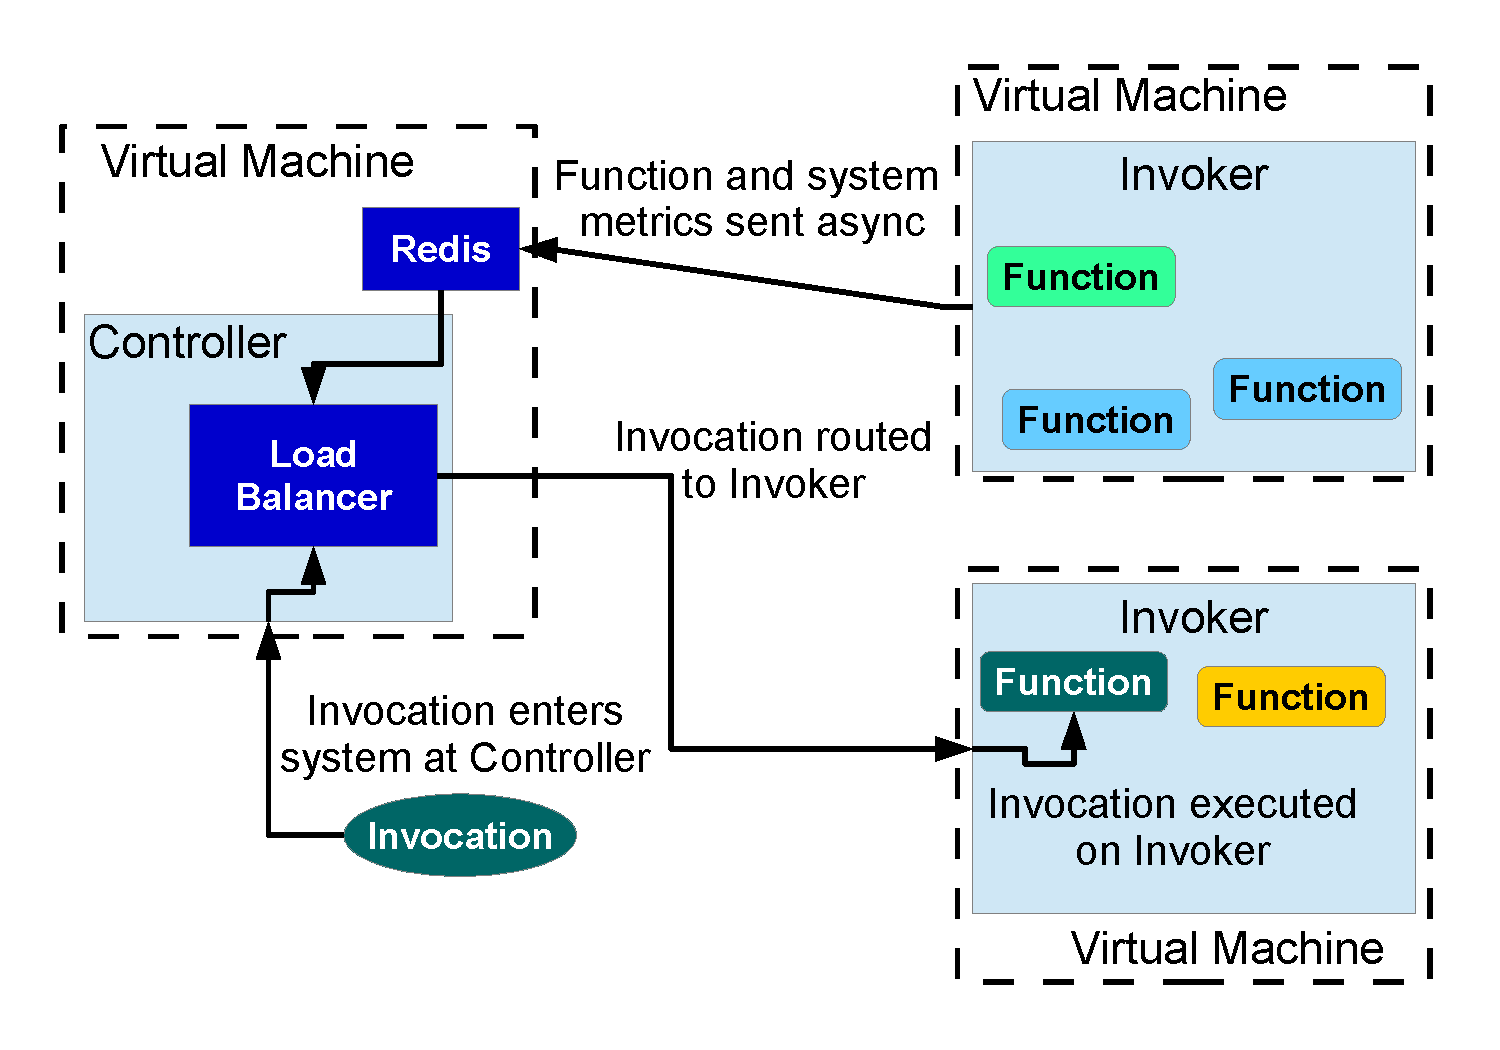
\includegraphics[width=0.6\textwidth]{chrlu/faaslb-osdi22/figs/sys-diag.pdf}
 %   \vspace*{-0.3cm}
  \caption{System diagram of relevant OpenWhisk components and communication used to schedule and run function invocations.}
  \label{fig:sys-diag}
  %  \vspace*{-0.3cm}
\end{figure}

The CH-RLU algorithm described in the previous section requires two main additional pieces of information from each invoker/server: the load averages, and the cold/warm running times of functions. 
Both of these are periodically (every 5 seconds) captured and stored in a centralized redis key-value store.
The load-balancer in the controller reads these asynchronously: working with stale and inconsistent metrics is our key design goal. 
The default load-bound, b, is 1.2, and the max load, b\_max is 6. Popularity threshold is set to 20\%.
We did not observe performance to be very sensitive to these parameters, and thus do not need to auto-tune them, and they are suitable as user-inputs. 

%\vspace*{-0.2cm}
\subsection{Performance Optimizations For OpenWhisk}

Since our goal is to run functions under high load, we ran into a large number of OpenWhisk performance and scalability bottlenecks.
We found default OpenWhisk to be almost unusably slow and unstable even under reasonable load. 
We present their details and our actions to overcome them, hoping that the fast-growing serverless computing research field can benefit from our lessons. 


In our experience, the primary source of scalability bottlenecks when concurrently managing Docker containers.
We found significant contention in \texttt{dockerd}, Docker's control daemon which handles all the container lifecycle events.
Even at moderate loads (normalized server load average close to 1), high dockerd contention can increase tail latencies by \emph{several minutes!}


Currently, OpenWhisk \textbf{pauses} each container after function execution, which prevents it from being scheduled by the CPU.
It then resumes the container before running the next invocation of the same function (assuming a warm start).
Each invocation therefore requires these two additional (pause/resume) events to be handled by dockerd, which results in significant lock contention.
Because of the FaaS programming model, the pausing is not necessary, since nothing in the container can run after a function has returned.
Therefore, we remove these redundant pause/resume operations to reduce dockerd contention.
This reduces the OpenWhisk overhead by 0.2 seconds \emph{per-invocation} on average.
More importantly, by reducing dockerd contention, we were able to run a much larger number of concurrent functions. 

An even larger source of scalability bottleneck is \textbf{network} namespace creation time.
Using the default bridge networking requires each invocation to create a new TUN/TAP network interface.
We found this to be a very expensive operation because of Linux network stack overheads (several 100 ms), and because of dockerd's userspace lock (futex) contention for its networking database. 
We found that as the \emph{historical} total number of containers launched grows, so does the size of the network-interface database.
Dockerd reads and updates this database under the critical section, and the larger database results in higher lock contention.
As a result, we were unable to use VMs/servers with more than 4 CPUs after 20 minutes of sustained load, since the dockerd contention resulted in many functions timing out (timeout was 5 minutes)! 

We sidestep this problem by not using bridge networking, but instead using Docker's \textit{host} network option and assigning each container a unique port on the host. 
Implementing the network change required updating the OpenWhisk runtimes used to wrap functions to monitor their specified port.
This change allowed us to run functions on larger invokers and under more sustained load, and eliminated most timeouts. 

Finally, after a certain request rate threshold, we found the default \texttt{nginx} OpenWhisk frontend would crash and return \textit{502 BAD GATEWAY} for all URLs. 
We did not discover the cause of this problem, and simply bypassed it by letting function invocations to communicate with the controller/load-balancer directly. 

\noindent \textbf{CPU limits.} 
OpenWhisk uses the \textit{-{}-cpu-shares} option to set container CPU priority.
This has an unintended consequence of allowing functions to use more than one CPU core while running.
Major FaaS providers constrain functions to a single core unless they have extremely high memory allocations (<1 GB).
In order to stay in line with providers and prevent outsized impact on system load from some functions, we use the \textit{-{}-cpus} flag instead to assign each function no more than one CPU.

Together, these performance optimizations have allowed us to run OpenWhisk on invokers that are $4\times$ larger, and serve more than $6\times$ the load, without dropping functions due to timeouts.
%
We plan to upstream all these performance optimizations in OpenWhisk to provide a higher-performance and lower-jitter control plane for FaaS research and production deployments. 

\begin{comment}
\noindent \textbf{docker pause.} 
OpenWhisk pauses Docker containers after each invocation completes to prevent the user code from continuing to run.
We disable this pausing because it causes significant contention inside Docker, affecting both latency and the ability to run more concurrent functions on an individual server.
Because we control the code running inside all our functions, we do not need the pausing as a security concern or to limit impact on load.
Our functions do not do anything outside of an invocation.

\noindent \textbf{configuration.}
While OpenWhisk provides a large number of configurable settings, most of them are locked into files.
In order to make the settings more amenable to prototyping and rapid changes, we converted many of them to also work as injectable environment variables.


\end{comment}



% SPACE: can be safely removed to get space back
% OPTIMIZATION
%Finding the consistent hash node a function hashes to is a relatively expensive operation, so we simply cache these pairs for fast lookup.
% Any time we change the hash ring (i.e. an invoker comes or goes) we simply empty the cache and allow it to refill as requests come along.


% SPACE: can be safely removed to get space back

% \begin{enumerate}
%   \item docker contention
%   \item host network
%   \item OW usage of docker CPU limits
%   \item general significant OW overhead
%   \item skip nginx
%   \item make many settings configurable
% \end{enumerate}

% OW Overhead median = 0.05472302436828605 seconds
% ShardingContainerPoolBalancer [0.0215673  0.05472302 0.86742063 4.59444914 6.49693995]
% quantiles: [0.1, 0.5, 0.8, 0.90, 0.99]


\section{Evaluation}
\label{sec:chrlu-eval}
In our evaluation we present the effectiveness of our load-balancing policy (RLU) using an implementation in OpenWhisk. 
Our primary goal is to quantify the impact of different load-balancing policies on function latencies under varying load conditions. 


% \begin{enumerate}
% \item Networking overhead 
% \item Pause-unpause overhead
% \item System overheads
% \item Effect of concurrency 
% \item Function latency vs. load 
% \item Default LB vs. Us
% \item TTL vs. GD
% \end{enumerate}

%  \vspace*{-0.2cm}
\subsection{Evaluation Environment}

\begin{figure}
  \centering
  \subfloat[Global Latency Impact]{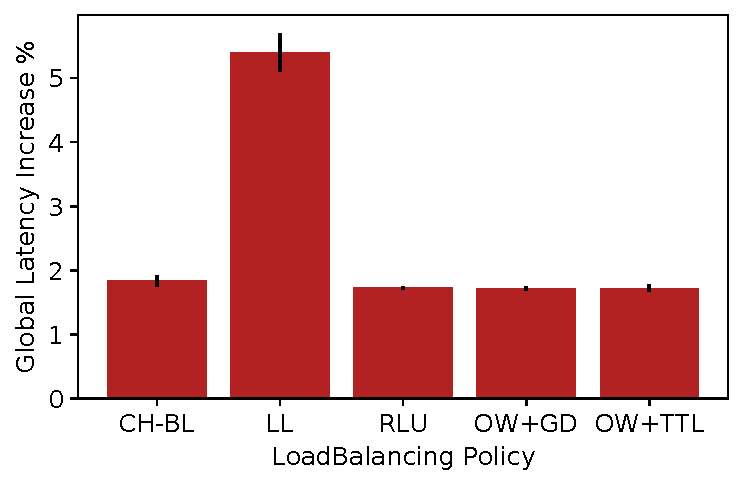
\includegraphics[width=0.5\textwidth]{chrlu/faaslb-osdi22/figs/compare/20-global-latencies-cntnorm.pdf} \label{fig:20-normalized-latencies}}
  \subfloat[Invocation Throughput]{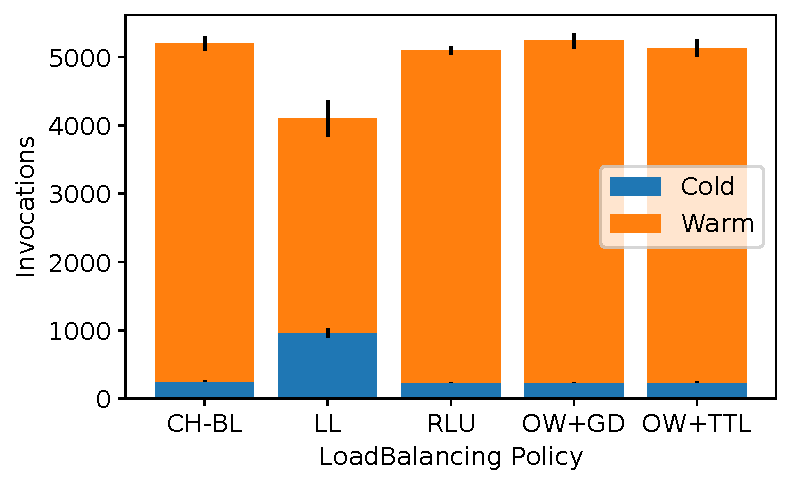
\includegraphics[width=0.5\textwidth]{chrlu/faaslb-osdi22/figs/compare/20-invokes-ttl.pdf} \label{fig:20-invokes}}
 % \vspace*{-0.5cm}
  \caption{Latency and throughput under low-load. Locality-agnostic least-loaded policy has more cold starts and a higher impact on latency.}
  \label{fig:low-load}
\end{figure}


\noindent \textbf{HW and SW Config.}
We run OpenWhisk in a distributed mode across 9 VMs.
8 invokers are each in their own VM with 16 vCPUs and assigned to use 32 GB RAM for hosting functions.
The final VM hosts the controller, load-balancer, and remaining services, with 12 vCPUs and 50 GB RAM to ensure it is not a bottleneck.
Metrics about system load were captured every 5 seconds by calling \textit{uptime} on each invokers VM and normalized by the number of CPUs on that system.
All latency information was recorded by the client, timing the HTTP request until the request completed. 
%
We make no policy changes to the invoker eviction policy, but use the changes from FaasCache~\cite{faascache-asplos21} for eviction decisions on the invoker.

\noindent \textbf{Contenders.}
In addition to our proposed load balancing policy, we compare against the default OpenWhisk load balancing policy (described in Section~\ref{subsec:ch}) with GreedyDual (OW+GD) and 10 minute Time-To-Live (OW+TTL) eviction policies, and implement two other load balancing polices for comparison: least loaded (LL), and consistent hashing with bounded loads using stale load-averages (CH-BL). 
For CH-RLU and CH-BL, we set the $max\_chain\_len=3$, a high max load bound, $b\_max= 6$, and a popularity threshold, $p=20\%$. 
We did not find performance to be particularly sensitive to the load-bound: the function latencies showed little changes across load upper-bounds of $[2-8]$. 
% This is also shown earlier in our latency vs. load analysis in Section~\ref{subsec:function-perf}. 

% $bounded\_ceil = 6$ because of the low correlation between a function's latency and server load from 


%%%%%%%%%%%%%%%%%%%%%%%%%%%%%%%%%%%%%%%%%%%%%%%%%%

\noindent \textbf{Metrics.}
%Evaluating the quality of a serverless load balancing policy can be done using several metrics.
We examine three main metrics: cold starts, the global average latency across all invocations, and the evenness with which load is spread amongst workers.
%
The first two directly and obviously relate to end user service quality but the third is more intricate. 
Providers pay for servers to run functions on and don't want those resources going unused and therefore wasted.
Equally, a server that is overloaded (not enough CPU or memory resources) will cause a spike in end user latency due to contention of queuing.
%
To quantify the global impact on latency from placement decisions, we normalize each invocation's latency by the ideal (minimum) latency, take the per-function mean of these, multiply each mean by the percentage of invocations that function had in the whole trace, and finally take the mean of those function latency means.
This is essentially a weighted average of latency-increase (i.e., slowdown).
It gives some balance between outcomes, for example, a rare function may get several bad placement decisions and thus increase the global latency, or a very common function generally has warm hits and does not impact latency. 
%With this metric we get a specific percentage of the increase in latency that load balancing policies have over the theoretical optimal in which all invocations have their minimum runtime.

% Setup:
% Custom OpenWhisk run on self-hosted VMs
% 8 invokers with 16 vCPUs and assignedto use 32 GB RAM for hosting functions
% Other services on 9th VM with 12 vCPUs and 50 GB RAM.


\begin{figure*}%[ht] 
  \centering
  \subfloat[Latency]{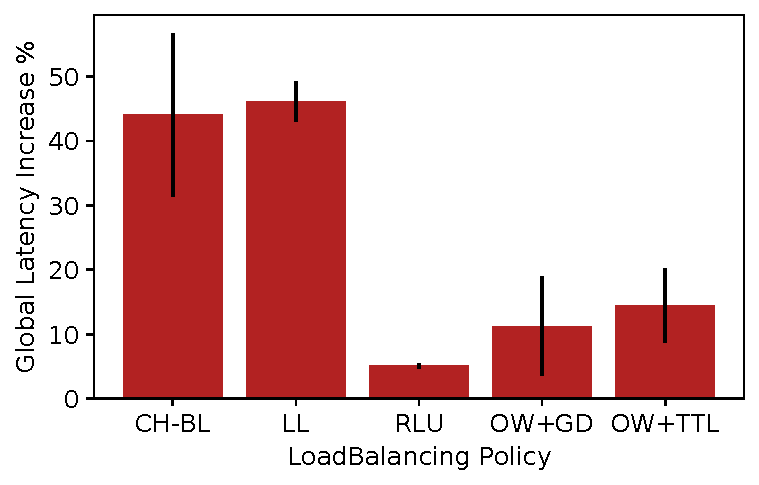
\includegraphics[width=0.4\textwidth]{chrlu/faaslb-osdi22/figs/compare/120-global-latencies-cntnorm.pdf} \label{fig:120-normalized-latencies}} 
  \hfill
  \subfloat[Throughput]{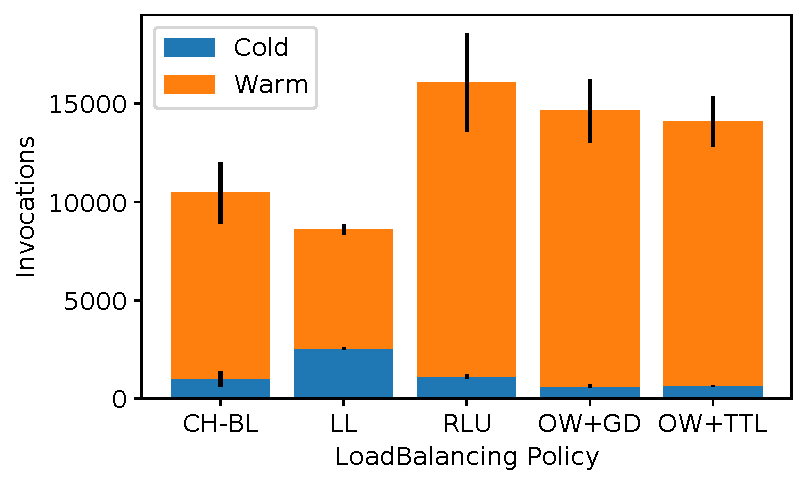
\includegraphics[width=0.4\textwidth]{chrlu/faaslb-osdi22/figs/compare/120-invokes-ttl.pdf} \label{fig:120-invokes}}
  \hfill
  \subfloat[Server Load variance]
  {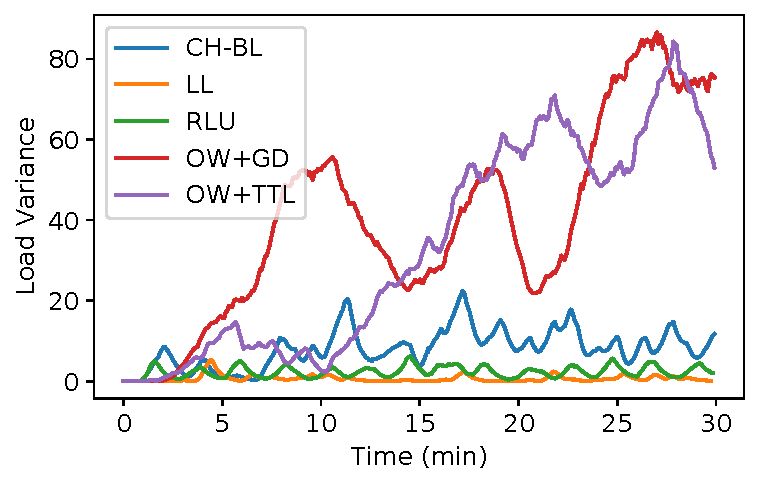
\includegraphics[width=0.4\textwidth]{chrlu/faaslb-osdi22/figs/compare/3-120-loadAvg-variance.pdf} \label{fig:120-load-variance}}
 % \vspace*{-0.5cm}
  \caption{At high server loads, our RLU policy reduces average latency by 2.2x at higher throughput, compared to OpenWhisk's default policy. It does so by keeping cold starts and load-variances low.}
  \label{fig:high-load}
\end{figure*}


\noindent \textbf{Workload.}
We convert 12 functions from FunctionBench~\cite{kim_functionbench_2019} to run on OpenWhisk.
To create a more realistic variety of functions, we create ten copies of each function with unique names, giving us 120 unique functions. 
Each function clone is invoked at different frequencies mimicking the arrival frequencies of the Azure trace~\cite{shahrad_serverless_2020}. 
% We picked these to mimic the invocation disparity shown in real-world traces.
Our load is generated using the closed-loop load generation tool Locust~\cite{locust} to invoke functions, running 20 threads for low load, and 120 for heavy load stressing.
Locust cannot easily have dedicated threads to invoke each function, so we convert the ``frequencies'' into weights and use those to randomly choose what function will be invoked next.
Each thread will iteratively invoke a random function, and after its completion wait 0-1 seconds before invoking another function.
Unless stated otherwise all experiments are run with the above settings, under heavy load, for 30 minutes, and results are the average of 4 runs.

% Workload:
% Load generated by locust
% 50 threads running in closed loop load generation (unless stated)
% 12 functions converted from FunctionBench
% mix of function types, both in runtime and resource usage
% each uploaded 4 times with unique names
% These 4 different ones will be called with diff frequencies of 1, 5, 16, 40
% mimic the invocation disparity displayed in Azure Function trace
% giving us 48 functions to call
% Load applied for 30 minutes. System stable by then and enough for a TTL impact
% each experiment run 4 times, and graphs are the average of those runs, unless stated

\begin{comment}
\subsection{Function Jitter}

\label{sec:unstable-latency}
This system added latency instability combined with the initial cold start overhead for a function's first run are two overheads no load balancing policy can mitigate.
% maybe TODO: Something on on we can only optimize warm hits and server load impact on runtime and will always have "added latency" over the optimal.

To see how our functions' latencies are affected by the system under load, we adjust the setup to have a single invoker and slowly crank up the number of threads making requests to increase the load on that invoker.
Latency increases due to load come from two causes: 1) CPU contention increases function execution time and 2) the server marshalling resources to run the function and extract results.
Figure~\ref{fig:LatencyVsLoad} shows a representative selection of functions, and the latency of individual invocations in relation to the load of our single invoker when they were invoked.
One mixed CPU and disk bound load performing web serving in Figure~\ref{fig:CHAM} sees \textit{no} impact at extreme loads.
Its only latency outliers are due to the inconsistent system overhead we saw above.
A more CPU intense function performing AES key encryption and decryption in Figure~\ref{fig:AES} roughly has some correlation with load.
Once the load gets above \textbf{8} does it not finish near its minimum latency anymore.
The AES function also exhibits layency inconsistency from the system like 'float' did, with many of the invocations under the extreme load of 10 taking as long as invocations with no load.
% Both~\ref{fig:AES} and~\ref{fig:FLOAT}, both CPU bound functions, see \textit{no} impact at extreme loads.
Finally, the long running and CPU bound Sklearn training function in Figure~\ref{fig:TRAIN} is marginally affected as load becomes extreme.
There is a definite correlation between the two, but it is clearly not linear, with a normalized load of 10 only causing a 1.5x increase in function latency.
These results challenge the traditional notion that functions are strictly limited by CPU resources. %, but we see that this isn't true.
We can favor locality more than load, allowing us to both prevent cold starts and not increase latency on warm starts.
Knowing that functions can withstand high server load up to a point, for all our following experiments we set the load bound used by RLU to 6.

\end{comment}


  %\vspace*{-0.2cm}
\subsection{Load-balancing Performance}
\label{sec:policy-comare}

% Policies being compared:
% Ours
% Bounded Loads
% Least loaded
% OpenWhisk (memory sharding) + GD
% OpenWhisk (memory sharding) + TTL

% Lots of metrics to consider when deciding a 'good' policy
% Classic cold start %
% function throughput 
% aggregated function latency
% distribution of load
%   resource usage on invokers

% The quality of a load balancing can be demonstrated in many different ways, and the addition of serverless workloads makes it more complicated.
% Our fixed-time and closed-loop load allows us to examine key metrics for FaaS and load balancing policies in general.


% global normalized latencies for 120 as a percentage over ideal
% ['CH-BL', 'LL', 'RLU', 'OW+GD', 'OW+TTL']
% [44.03687355782084, 46.12511623486831, 5.08886752197281, 11.27379780859461, 14.4173988318167]

% global normalized latencies for 20 as a percentage over ideal
% ['CH-BL', 'LL', 'RLU', 'OW+GD', 'OW+TTL']
% [1.83828219306087, 5.397093279722829, 1.7271133329324055, 1.7177648275920407, 1.723332172907966]

% Stable load
% Compare functions w/20 threads
% 20-compare-functions-ShardingContainerPoolBalancer-RLULFSharding.pdf 0.9997180360888229
% 20-compare-functions-LeastLoadBalancer-RLULFSharding.pdf 2.6262500335629335
% Compare functions w/120 threads
% 120-compare-functions-ShardingContainerPoolBalancer-RLULFSharding.pdf 1.7029922705698093
% 120-compare-functions-LeastLoadBalancer-RLULFSharding.pdf 7.805708861373892

When we run them under \textbf{light load} in Figure~\ref{fig:low-load}, the policies that use a locality mechanism are essentially identical.
The load on any one server is never high enough to impact co-located functions and we never have to forward invocations and incur excess cold starts, giving us a \quotes{lower bound} on load balancing.
The low 1-2\% latencies in Figure~\ref{fig:20-normalized-latencies} we see here are due to initial cold starts for functions and the varied overhead imparted by the system analyzed earlier.
The least loaded policy is significantly worse as it's lack of locality causes excessive cold starts as evidenced by the high number of cold starts in its invocation results detailed in Figure~\ref{fig:20-invokes}.
% The global latency impact in Figure~\ref{fig:20-normalized-latencies} and invocation throughputs in Figure~\ref{fig:20-invokes} 


Next we run the policies under our \textbf{heavy load} scenario, and get a clear distinction between how each of them performs. 
The two versions of OpenWhisk  in Figure~\ref{fig:120-normalized-latencies} only increase latency by 11\% and 14\% respectively which is rather good.
They cannot complete with RLU whos increase is less than half of that, a tiny 5\% impact on global latency.
CH-BL and least loaded increase global latency by over 40\%, showing terrible performance in that metric and on invocation throughput. 


The wide gap between policies can be understood by comparing the load variance between their workers (Figure~\ref{fig:120-load-variance}).
OpenWhisk's default policy is to only move a function to another server if the ``home'' one does not have available memory to run it. 
While very good for locality (getting fewer cold starts than RLU in Fig~\ref{fig:120-invokes}), it creates severe imbalance on the worker loads.
A few workers grow to extremely high load and their functions suffer, while others are mostly empty. 
RLU intelligently forwards invocations when a worker is near overload, keeping load variance low while protecting locality. 
Least loaded actually does the best at keeping equal load amongst workers, but at the cost of poor locality.

% An important seconday goal is to full utilize worker resources and ensure that certain workers are neither over- nor under-loaded compared to each other.
% The default OpenWhisk policy does a poor job of keeping load even on its workers, as shown in Figure~\ref{fig:OW-loadavg}
% Several workers have a load near 0, and one has a load of over 10!
% While the system has a stable mean load denoted by the solid black line, the dashed variance line is always extremely high.
% Our policy, shown in Figure~\ref{fig:Forward-loadavg} has a similar mean load to that of OpenWhisk, hovering just under 2.
% It differs by having a substantially lower variance, keeping invoker CPU load close together.
% For example invoker 4, the purple line, reaches a load of 4x at points but the system forwards work to other invokers and the load stabilizes.

%  \vspace*{-0.2cm}
\subsubsection{Handling Bursty Traffic}

% Two of the high-frequency functions have their frequency quadrupled and returned to normal every 10 seconds
% aes and gzip specifically, CPU and disk/cpu intensive respectively


\begin{figure}
  \centering
  \subfloat[Global Latency Impact]{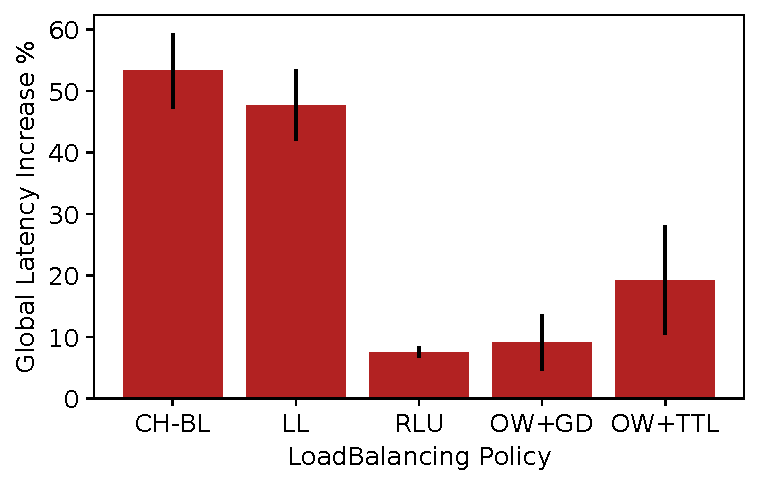
\includegraphics[width=0.5\textwidth]{chrlu/faaslb-osdi22/figs/bursty/120-global-latencies-cntnorm.pdf} \label{fig:bursty-latencies} }
  \subfloat[Worker Load Variance]{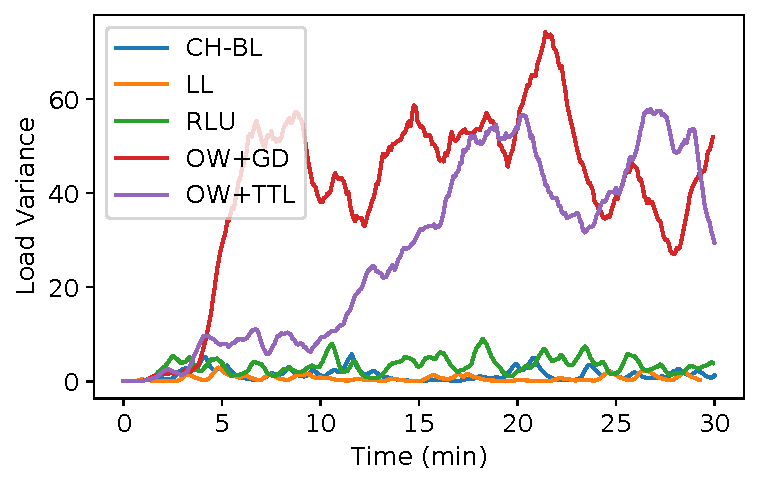
\includegraphics[width=0.5\textwidth]{chrlu/faaslb-osdi22/figs/bursty/3-120-loadAvg-variance.pdf} \label{fig:bursty-variance} }
%  \vspace*{-0.4cm}
  \caption{RLU improves latency by 10\% compared to OpenWhisk under bursty load conditions, while keeping a low worker load variance.}
  \label{fig:bursty-closedload}
\end{figure}


% Bursty load, 120 threads
% 120-compare-functions-ShardingContainerPoolBalancer-RLULFSharding.pdf 1.0932351152955206
% 120-compare-functions-LeastLoadBalancer-RLULFSharding.pdf 6.784717290259041

% global normalized latencies for 120 as a percentage over ideal
% ['CH-BL', 'LL', 'RLU', 'OW+GD', 'OW+TTL']
% [53.31502690829111, 47.720802127692316, 7.542333155555457, 9.089841768309597, 19.267038417080776]

\begin{figure}
  \centering
  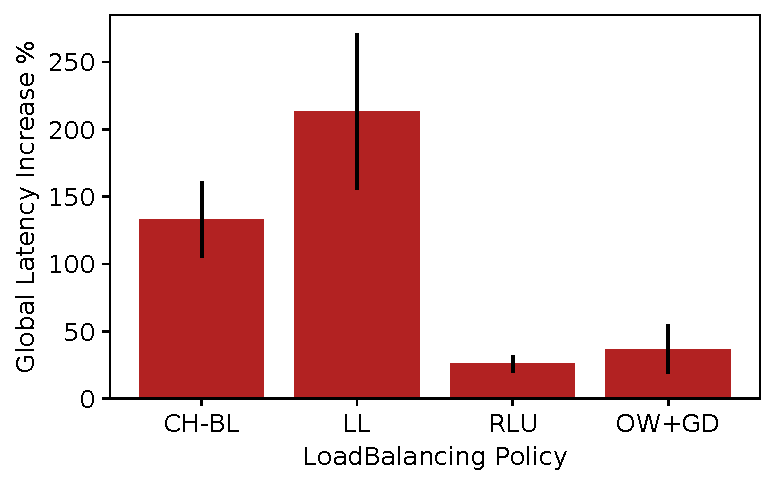
\includegraphics[width=0.6\textwidth]{chrlu/faaslb-osdi22/figs/ow/openload/openload-latencies-cntnorm.pdf}
 % \vspace*{-0.3cm}
  \caption{Global latency impact under a 30-minute long rising burst load from an open-loop generator. RLU reduces  latency by 17\% compared to OpenWhisk.}
  \label{fig:bursty-openload}
 %   \vspace*{-0.3cm}
\end{figure}

Next we take two different bursty workloads to see how the polices handle changes in invocation patterns.
The first uses the same closed-loop load generation but adjust the weights by which functions are invoked.
Every 30 seconds two of the top weighted functions are chosen to become bursty, and have their weights set much higher.
At the end of a burst their weights are returned to normal and another two functions are chosen.
As can be seen in Figure~\ref{fig:bursty-latencies} our policy acheives a 17\% lower impact on global latency than OpenWhisk with GreedyDual.
RLU represents a 60\% reduction to latency over OpenWhisk with its default TTL backend.
The more advanced eviction decision choices have a clear effect on improving the system even when the load balancer does not optimize for it.
The longer running functions in our workload have a larger effect on system load and the load balancer must be aware of this impact and either spread that heavy popular function around or move other functions off of that server.
Again, OpenWhisk does not take load into account and severely overloads some servers while languishing others.
We see more sky-high load variances from this bursty workload in Figure~\ref{fig:bursty-variance}.
Policies that monitor load, our RLU, CH-BL, and least loaded keep tighter control on load variance.

% We do suffer more cold starts, caused by moving traffic across workers to avoid load spikes from the bursty workloads.
% OpenWhisk does not try to mitigate variable workloadsd and suffers accordingly. 

% global normalized latencies for open load generation
% ['CH-BL', 'LL', 'RLU', 'OW+GD']
% [140.53344802991816, 228.83239333263217, 25.886003912929013, 36.857319393171736]

The second busrty load is a 30 minute long-rising burst, starting with just a few invocations per second and reaching a sustained peak of roughly 18 invocations per second at roughly 25 minutes.
We generated this load with a custom open-loop load tool that fires invocations but does not block waiting for completion.
New invocations are continually fired in a preset pattern of function types and times.
The global latency impact of this final scenario can be seen in Figure~\ref{fig:bursty-openload}.
Only the final 10 minutes of the workload place the system under extreme load, and the differences between policies reflect this.
CH-BL and least loaded cannot keep up with the suddenly changing load, causing a latency increase of over 100\% and 200\% respectively.
RLU's 25\% increase in global latency is still significantly better, 30\% lower, than OpenWhisk.
Our policy is able to make ideal choices for function placement under a varient of realistic workload scenarios.

\subsubsection{Scaling}
\begin{comment}
\begin{figure}
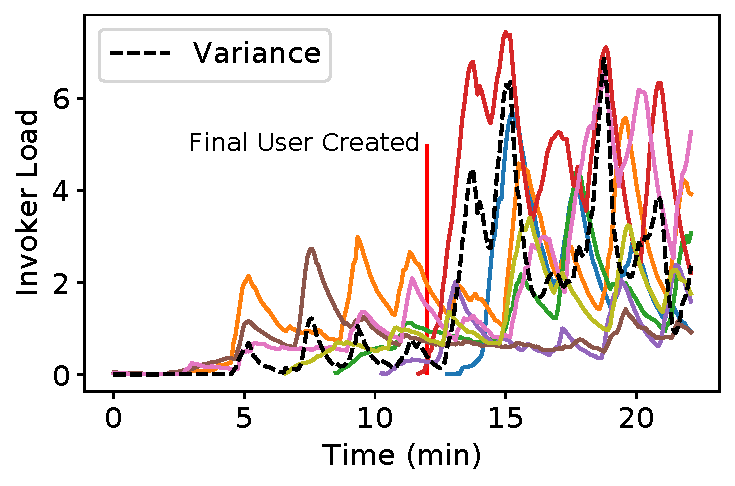
\includegraphics[width=0.33\textwidth]{../figs/scaling/120-loadAvg-6sec.pdf}
  % \vspace*{-0.3cm}
  \caption{When load increases over time, new workers are spun up and recieve a share of the workload while not being overloaded.}
  \label{fig:scaling}
%\vspace*{-0.3cm}
\end{figure}
\end{comment}

\begin{figure}  
  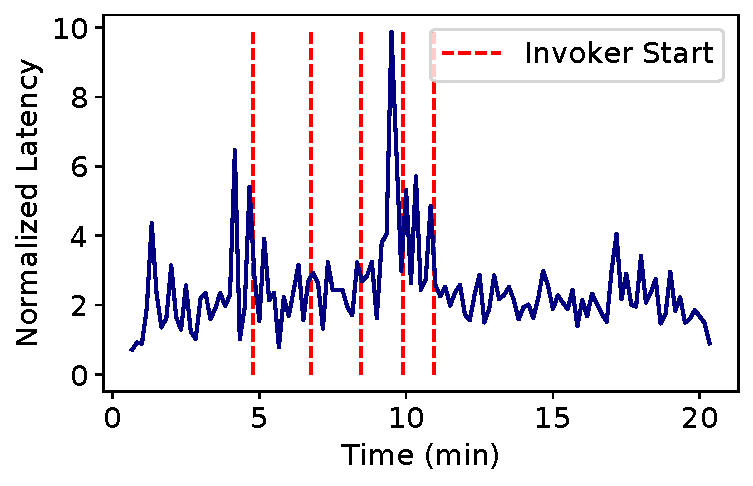
\includegraphics[width=0.6\textwidth]{chrlu/faaslb-osdi22/figs/scaling/scaling_lat_over_time-nolabel.pdf}
%  \vspace*{-0.3cm}
  \centering
  \caption{The average normalized function latency over time for a dynamic workload. New invokers are launched at the dashed lines, keeping the latency in check.}
  \label{fig:scaling-latency}
%  \vspace*{-0.3cm}
\end{figure}


% we are able to scale up infrequently and well
% system handles load as if all invokers were always up

% As described in Section~\ref{}, we can intelligently scale our systems workers as demand increases.
Lastly we want to demonstrate how our policy reacts to scaling the number of workers as demand increases.
We start our cluster with only 3 invokers and increase applied load up to the heavy load scenario above.
Rather than starting with the 120 threads of the heavy load with this smaller cluster, we adjust the scenario to start with a single thread and add a new one every 6 seconds, reaching the final thread count at about minute 12.
% Our small cluster does not allow us to match the multi-server scaling up and down changes of the simulator, so here we turn on invokers when there is an increase in forwarding to server servers beyond the 'home' server.
%The results for a single run of this scaling are in Figure~\ref{fig:scaling} with each invoker being represented by a unique color.

As the average invoker load increases, the controller activates a new worker and starts directing work towards it.
New workers are kept under the load bound of 6 and see load similar to our previous experiments that had a constant load.
%We can also correlate when new invokers are started to the latency invoked functions are encountering.
Figure~\ref{fig:scaling-latency} shows the function latencies (normalized to respective min. warm times). % and average them in 5 second groups. 
Preceeding each worker being started is a rise in overall latency, which then falls after the invoker has come online and starts taking additional load.
Thus, our horizontal scaling is able to dynamically keep the function latency in check, even though it only uses coarse-grained server load metrics.

% The remaining 5 workers are started dynamically, and quickly have a load similar to already existing workers.
% There are not load spikes or troughs, indicating the work is being spread well to new invokers as time moves on.
%These graphs are not a combination of multiple runs, but are characteristic of the performance across runs.

%\vspace*{-0.2cm}
\subsubsection{Load-balancer Overhead}

% BoundedLoadsLoadBalancer: 0.0001106853074066166
% LeastLoadBalancer: 6.170695498725195e-05
% RLULFSharding: 0.0001242685814681948
% ShardingContainerPoolBalancer: 4.7238211672012455e-05

More complicated routing decisions naturally mean they are more computationally expensive to perform.
% We have been able to keep balancing decisions to roughly 1 ms thanks to the optimizations described in Section~\ref{sec:impl}. 
Even so, RLU is on significantly slower making individual routing decisions, taking on average $1242.6 \mu$s to OpenWhisks' $472.3 \mu$s.
Such times represent a fraction of the time spent per-request by the system and is made up for by our more optimal placements. 


% %\vspace*{-0.3cm}
\subsection{Simulation Evaluation}
\label{subsec:eval-sim}


  \begin{figure}
  \centering
  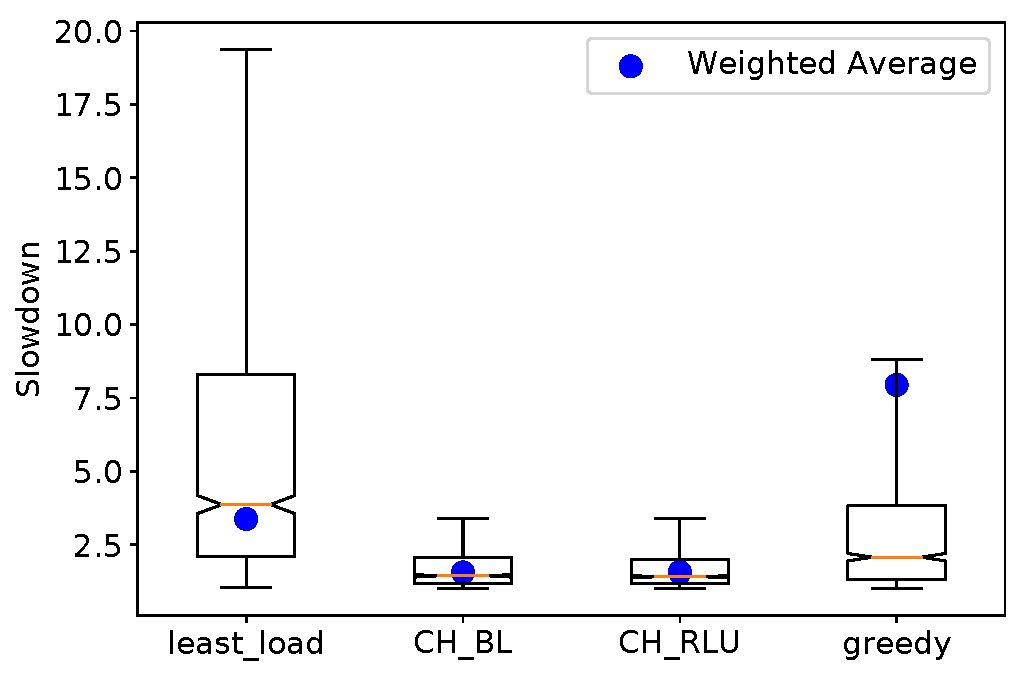
\includegraphics[width=0.3\textwidth]{chrlu/faaslb-osdi22/figs/1k/latencies-GD.pdf}
%  \vspace*{-0.3cm}
  \caption{[Simulated] Function latency distribution. }
  \label{fig:1k-lat}
%  \vspace*{-0.3cm}
  \end{figure}

\begin{figure}
  \centering
  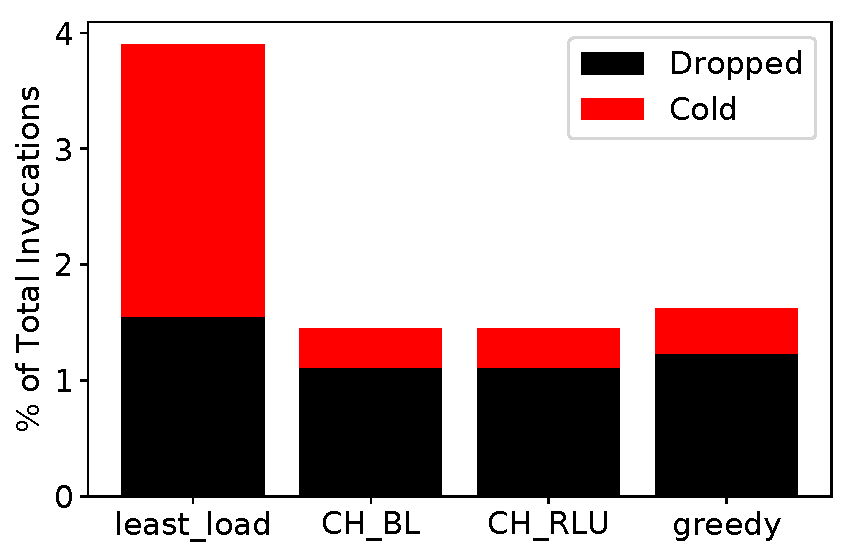
\includegraphics[width=0.3\textwidth]{chrlu/faaslb-osdi22/figs/1k/cd-GD.pdf}
%    \vspace*{-0.3cm}
  \caption{[Simulated] Cold and dropped functions.}
  \label{fig:1k-cd}
%    \vspace*{-0.3cm}
\end{figure}


To investigate the performance of various load-balancing policies at larger scales, we use a simulation approach.
We have developed a discrete-event simulator, which plays a function workload trace, and emulates the various aspects of function execution and slowdown: slow/warm starts, slowdown due to concurrent processing by emulating a G/G/k queuing system on each server, and various load metrics (emulating Linux exponentially decaying load averages, stale loads, real-time loads, etc.). 
The simulator allows us to implement different policies using information that would not otherwise be available on a real system: accurate function cold and warm times, instant load information, etc.
The function running times are computed by adding the actual provider-captured running times to the OpenWhisk and Docker startup overheads that are empirically measured and modeled.
This, when combined with queuing delays, captures the overall slowdown due to concurrent processing.
The simulator is implemented in Python in about 3,000 lines of code. 

We run the Azure trace with 1000 randomly chosen functions spanning almost a million invocations, and compare different load-balancing policies.
This workload is highly bursty and is characterized by the Figures in Section~\ref{sec:challenges}. 
We have implemented a ``online greedy optimal'' policy that considers \emph{all} servers when running functions, by picking the server with the lowest expected running time (based on Section~\ref{subsec:chch}).
This would be impractical and unrealistic to implement, since it needs accurate information about every function's keep-alive status on every server, and an accurate model of function performance at various loads.
Nevertheless, it provides an optimistic baseline: our consistent-hashing based policy ($CH-RLU$) is significantly simpler, only considers a small subset of servers, and does not require omniscient cluster state. 

Figure~\ref{fig:1k-lat} compares this greedy policy with a locality-agnostic ``least-loaded'' policy that is popular in web-clusters, and the two consistent-hashing based policies. 
The figure shows the function slowdown factor for each function, as well as the global average slowdown.
Slowdown is defined as the ratio of function's execution time to its base warm time without any system overhead, resource contention, or queuing delays.
Most functions do poorly with the least-loaded policy: the median function slowdown is almost $4\times$, primarily because of high cold-starts.
Figure~\ref{fig:1k-cd} compares the cold and dropped statistics for the various policies.

Returning to Figure~\ref{fig:1k-lat}, both CH-BL and CH-RLU have comparable performance, with a median slowdown of $2.4$. 
Finally, and surprisingly, the omniscient greedy policy performs poorly: with the global slowdown approaching $7$.
The primary reason for this is because of the bursty nature of the workload: the greedy policy tends to pick the server with the least-loaded server that can run the warm function.
However because of stale load information, we see a \emph{herd effect} on the server, and this causes extremely high resource contention and latency, even though the number of cold-starts is small (compared in Figure~\ref{fig:1k-cd}). 


% \begin{centering}
\begin{figure}
  \centering
  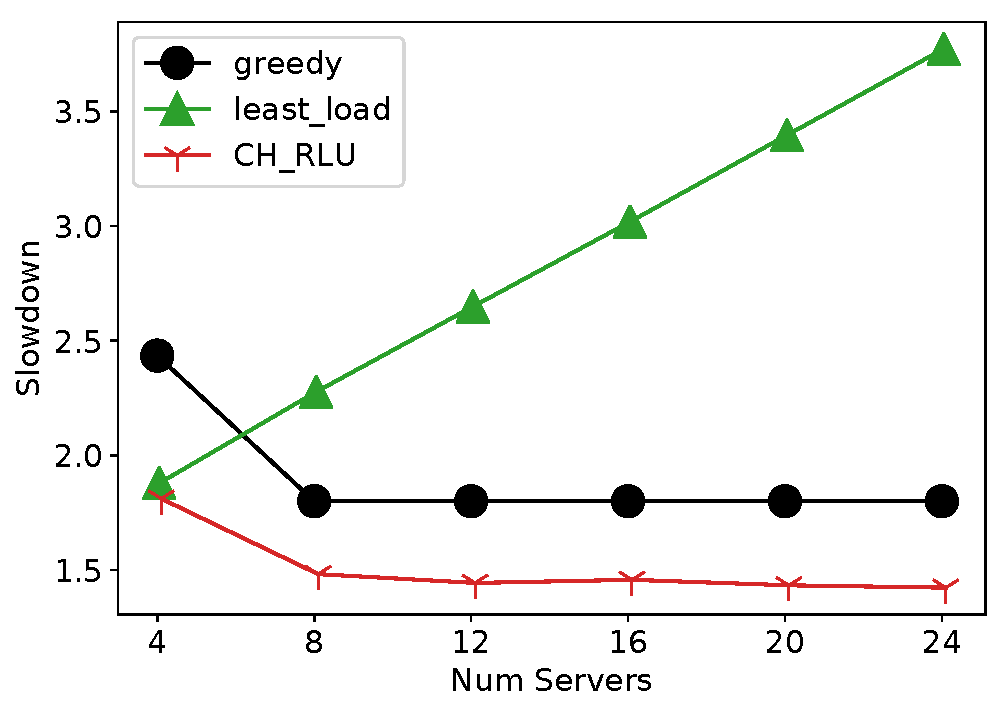
\includegraphics[width=0.3\textwidth]{chrlu/faaslb-osdi22/figs/1k/latencies-250scaling.pdf}
  %  \vspace*{-0.3cm}
  \caption{[Simulated] Function latencies as cluster size is increased. Least-loaded performs \emph{worse} because its locality and cold-starts become worse as more servers are added.}
  \label{fig:1k-scaling}
 %   \vspace*{-0.3cm}
\end{figure}
% \end{centering}

Finally, we investigate performance when the cluster size changes.
Figure~\ref{fig:1k-scaling} shows the slowdown for the three policies when the number of servers is increased.
Importantly, the total number of computing and memory in the cluster is kept constant at 256 CPUs and 512 GB, and the size of the individual servers is changed.
Thus 4 servers with 64 CPUs are compared with 8 servers with 32 CPUs, etc.
This experiment is intended to capture the effects of locality: smaller number of servers may have a higher hit-rate, and a more even load-spread.

Figure~\ref{fig:1k-scaling} shows how the function slowdown for both CH-RLU and greedy decays as the number of servers is increased.  
This is because larger servers see heavier lock and other resource contention, and thus while they may exhibit better locality, the load-induced slowdown dominates.
This has important ramifications for large FaaS providers, since they can continue using smaller servers for running functions, and expands the utility of small deflatable/harvestable VMs for running colocated functions~\cite{serverless-harvest-sosp21}.

CH-RLU reduces the function slowdown by 20\% compared to the greedy approach, across a wide range of cluster configurations in Figure~\ref{fig:1k-scaling}. 
Interestingly, least-loaded's performance worsens with increasing number of servers and fragmentation.
The main culprit is worsening locality.
With a small number of servers, least-loaded can get ``lucky'' and score a keep-alive cache-hit.
These fortuitous warm-starts get less probable with an increasing number of servers. 

%%% Local Variables:
%%% mode: latex
%%% TeX-master: "paper"
%%% End:




%~\cite{lbfaas-hpdc2022}

\begin{comment}
\begin{figure}
  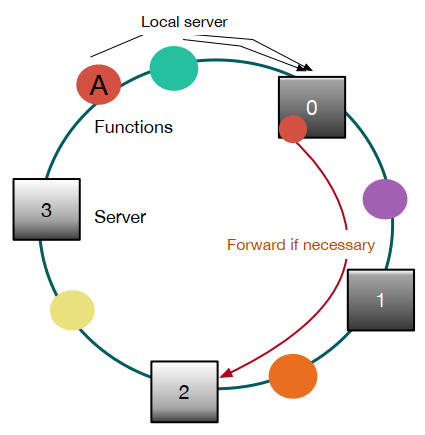
\includegraphics[width=.9\columnwidth]{./figures/consistent-hashing.png}
  \caption{Consistent hashing ring featuring function forwarding~\cite{lbfaas-hpdc2022}.}
  \label{fig:ch-rlu}
\end{figure}

In my work just accepted to HPDC~\cite{lbfaas-hpdc2022}, we take a different approach to load and locality balancing.
% Some functions are more \textit{popular} than others, and therefore will take up more system resources.
Previous work~\cite{shahrad2020serverless} revealed that a few functions make up the lion's share of invocations in FaaS systems.
Per Figure~\ref{fig:serverless-invocations} over 99\% of invocations are from just 19\% of functions, and load balancers need to take this pattern into account.
To start our balancing policy we use consistent hashing to always route a function to a home worker, favoring locality especially for those rarely invoked functions.
In the event a home worker is overloaded, we want to conditionally migrate work to other workers in an affinity-aware manner.
This load based migration locality is achieved by \textit{pushing} work around the has ring as shown in Figure~\ref{fig:ch-rlu}.
As a server's load increases, invocations are randomly pushed around the ring with popular functions being more likely to be forwarded.
This spreads work around preventing load imbalance, maintains locality for functions, and avoids latency increases from high CPU load on any individual worker.
\end{comment}

\chapter{\sysname: A Low-Latency FaaS Research Control Plane}
\label{chap:iluvatar}

Providing efficient Functions as a Service (FaaS) is challenging due to the serverless programming model and highly heterogeneous and dynamic workloads. 
% Great strides have been made in optimizing FaaS performance through scheduling, caching, virtualization, and other resource management techniques.
% The combination of these advances and growing FaaS workloads have pushed the performance bottleneck into the control plane itself.
Current open-source FaaS control planes like OpenWhisk introduce 100s of milliseconds of latency overhead, and are becoming unsuitable for high performance FaaS research and deployments.
In this chapter we present the design and implementation of \sysname, a fast, modular, extensible FaaS control plane which reduces the latency overhead by more than two orders of magnitude.
\sysname~has a worker-centric architecture and introduces a new function queue technique for managing function scheduling and overcommitment. 
\sysname~is implemented in Rust in about 13,000 lines of code, and introduces only 3ms of latency overhead under a wide range of loads, which is more than 2 orders of magnitude lower than OpenWhisk. 


\section{Why a new control plane?}
\label{sec:ilu-motivation}

We believe that the FaaS control plane is an important component of the modern cloud ecosystem, and presents many optimization opportunities and interesting research questions in system design. 

\textbf{Performance.}
%
Because of its central role in coordinating all aspects of function execution, the control plane plays a major role in determining function performance. 
Managing the function execution lifecycle for hundreds of concurrent invocations imposes a \emph{control plane overhead}, and increases the end-to-end latency.
This control plane overhead can be significant, and affects \emph{all} function invocations, including and especially the ``warm starts''. 
%Time spent in the control plane is simply measured by subtracting the execution time of the function code from the overall end-to-end latency.
% This overhead (end-to-end latency minus the function code execution time) for the PyAES function from FunctionBench~\cite{kim2019functionbench} is shown in Figure~\ref{fig:ow-scaling}. 

% The figure shows the 50 and 99 percentile overheads as the number of concurrent invocations are increased.
% In each case, we are invoking the function repeatedly in a closed-loop, and concurrent invocations are achieved by using multiple client threads.
% All invocations are warm starts.
% The experiment is run on a 48 core server (more details in Section~\ref{sec:ilu:eval}), and the figure thus shows the performance at low and medium load conditions. 

In experiments we witnessed OpenWhisk's 50 percentile latency overhead to be more than 10ms,  which is already a significant increase in latency for small functions which dominate real-world FaaS workloads.
Worryingly, the 99 percentile overhead is much higher, and rises to as much as 600ms, more details are in Section~\ref{sec:ilu:eval}.
To emphasize, for a median function in the Azure workload which runs for 500 ms, OpenWhisk can increase its latency by 100\%.  
Thus, the control plane plays a crucial role in function performance.
We note that these are the best-case warm-start latencies, when the function's containers is fully initialized and in memory. 
Since function cold-starts impose such a major performance penalty (increasing latency by more than $10\times$), mitigating them has been a major research focus. 
However, because of temporal and spatial locality of access, caching and prefetching techniques can be extremely effective, and the cold-start rate is often less than $1\% $ of all invocations~\cite{faascache-asplos21}. 
The majority of invocations are thus \quotes{warm}, where the performance is dominated by control plane overheads.

% We also see strange inversions in the scaling behavior: the overhead reduces for certain load-levels, and then increases again.
% This high overhead, high variance, and uncertain scaling behavior, results in many challenges for FaaS \emph{providers}. 
% Due to these issues, low-latency functions see severe performance degradation, and resource provisioning and capacity planning becomes harder due to the high variance and performance unpredictability. 

% Some of these latency overheads are an artifact of the architecture. 
% The shared Kafka function queue can be a major bottleneck; and there are no explicit backpressure or load regulation mechanisms, which is compounded by the CPU overcommitment. 

% For the sake of comparison, the figure also shows the latency overhead of \sysname~ in the same environment. 
% We are able to achieve a per-invocation mean overhead of less than 2ms for almost all the load conditions.
% Importantly, the tail overhead is also small: less than 3ms for less than 32 concurrent invocations, rising to 10ms when the system is saturated.

% To emphasize, for a median function in the Azure workload which runs for 500 ms, OpenWhisk can increase its latency by 100\%.  
% Thus, the control plane plays a crucial role in function performance.
% We note that these are the best-case warm-start latencies, when the function's containers is fully initialized and in memory. 
% Since function cold-starts impose such a major performance penalty (increasing latency by more than $10\times$), mitigating them has been a major research focus. 
% However, because of temporal and spatial locality of access, caching and prefetching techniques can be extremely effective, and the cold-start rate is often less than $1\% $ of all invocations~\cite{faascache-asplos21}. 
% The majority of invocations are thus ``warm'', where the performance is dominated by control plane overheads.
%\emph{We thus need a low-latency, low-jitter control plane.}

\textbf{System Design.}
%
As evidenced by the OpenWhisk architecture presented earlier, FaaS control planes are large, complex distributed systems.
% Due to the continually evolving needs of FaaS applications and emergence of new sandboxing techniques (such as lightweight VMs like Firecracker~\cite{firecracker-nsdi20}), they are sandwiched between the scale and heterogeneity of FaaS workloads on one hand, and the deep stack of OS and virtualization components on the other. 
%
A simple system running web services or microservices does not have to deal with sandbox management overheads, nor with highly heterogeneous request sizes.
% For reducing tail latency, these systems can often rely on the OS CPU scheduler for processor sharing, can do CPU allocation at very fine granularity~\cite{kaffes2019shinjuku}, use queuing theory techniques~\cite{prekas2017zygos}, etc. 
At the other extreme, control planes managing long running containers and VMs, like OpenStack or Kubernetes, face a much lower rate of VM arrivals and departures. and can do careful and \quotes{hard} resource allocation using bin-packing~\cite{cortez2017resource}.


Functions are highly heterogeneous, and can be seen as both latency-sensitive web requests \emph{and} large containers requiring significant system resources for several seconds. 
FaaS control planes thus have to do \emph{both} low-latency allocation \emph{and} pack CPU and memory resources on their servers carefully to maintain high system utilization.
Thus FaaS control planes are one of the more perfect microcosms of challenges in resource management and control in large scale distributed computing. 
%
% A clean-slate control plane design helps us investigate the fundamental performance tradeoffs and challenges in this fast-evolving ecosystem.
Our new implementation also helps to identify the current performance bottlenecks and new avenues of OS optimizations. 


\textbf{Control Plane for Experimental Systems Research.}
%
Performance-focused FaaS research is already challenging due to the extreme scale and heterogeneity of the workloads.
These challenges are compounded by existing control planes like OpenWhisk that are unfortunately highly unpredictable.
The control plane jitter and the extreme bimodal cold vs. warm latencies makes it difficult to do reliable and reproducible research~\cite{mytkowicz2009producing}, and subtle environmental and configuration effects can mask the true effects of new research optimizations.
However, it continues to be a key component in developing and evaluating FaaS research~\cite{akkus_sand_2018, shahrad_serverless_2020, faascache-asplos21, faaslb-hpdc22, zhou2022aquatope, ensure-faas-acsos20, alzayat_groundhog_2022}. 
% With OpenWhisk, function performance can be severely affected by a myriad of configuration options, such as insufficient memory for CouchDB, networking configuration, Docker configuration, etc. 

Given the importance of the control plane, we want \emph{predictable} performance to a large degree. 
In our experience, research in FaaS is often hindered by the large overheads and complexity of existing control planes. 
Thus, \sysname~is designed from the ground-up to be lightweight and provide predictable performance under different conditions. 
Our system implementation can potentially accelerate the development of new optimizations, clarify our understanding of performance characteristics of this relatively new stack, and provide a control plane for robust experiments. 
With a robust control plane, the community can share knowledge and advances, while being able to compare against a well-known and trusted baseline.

All aspects of function execution are orchestrated by a FaaS \emph{control plane}, which are implemented by frameworks like OpenWhisk~\cite{openwhisk}.
For using a FaaS service, the user interacts with the control plane for registering and invoking functions, tracking their status, etc.
The control plane manages the resources of a cluster of servers, and schedules functions on to them based on its load-balancing policies.

%FaaS is a relatively new workload paradigm, and control planes are still evolving and maturing.
%OpenWhisk is a popular framework which has been used as a platform for investigating and optimizing many facets of FaaS execution.

In OpenWhisk, user requests for invoking a function go through a reverse proxy (NGINX) to the central \emph{controller}, which implements, among other things, load-balancing (a variant of consistent hashing with bounded loads by default).
The controller puts the function invocation request into a shared Apache Kafka~\cite{kafka} queue.
Inside the worker, the invoker service pulls function invocations from the Kafka queue based on that worker's own resource availability.
Docker containers running a Go-based control plane agent are used to isolate functions, and each worker maintains a container pool of initialized/warm containers.
% A worker ultimately runs the function, and the control plane extends across the worker as well. 
%OpenWhisk strives to provide exactly-once semantics (although this hasn't been tested or verified) by logging function results in CouchDB. Kafka and CouchDB in the critical path. 
OpenWhisk logs function results in a CouchDB instance.
Importantly, both Kafka and CouchDB are on the critical path, and add 100s of ms to invocation latency.
%
OpenWhisk is highly modular and distributed, with many networked services.
All of these, combined with the JVM GC (it is implemented in Scala), results in large and unpredictable latency spikes~\cite{faaslb-hpdc22, hotcarbon22-faas}, with slowdowns of more than $10,000\times$ reported~\cite{zuk_call_2022}. 
%For instance, Stretch factors shown in \cite{zuk} of 10,000, indicating that the overhead is 10,000 more than the actual processing latency, and with response times of 100s of seconds. 

\begin{comment}
Shared kafka queue for scheduling and assignment of invocations.
Contended.
Ours simpler design: locality enforced through multiple independent loosely coupled components: CH-BL load balancer, and queuing at the invoker for tolerating bursts. 

The burst mitigation is done again using many techniques.
Increase queue size, overcommit resources and increase concurrency, forward, and finally elastic scaling.

OS level preemption is useful, since function invocation is not confined to a single process but many components such as containerization layer. The resource usage is also not uniform, but bursty and low average.

Stretch factors shown in \cite{zuk} of 10,000, indicating that the overhead is 10,000 more than the actual processing latency, and with response times of 100s of seconds. 

\noindent \textbf{Control planes}  (such as OpenWhisk~\cite{openwhisk})  handle all aspects of function execution. 
This control plane manages a cluster of servers to run functions on, and implements function scheduling, load-balancing, resource monitoring, function status tracking, storing function results, logging, etc. 
It is also responsible for performance optimizations for functions such as keep-alive~\cite{faascache-asplos21} to mitigate function cold-start overheads due to the sandboxing and function initialization overheads. 
%\emph{Paint a picture of what all it does.}
The control plane itself is highly distributed with many components such as API gateways, distributed message queues (such as Kafka), and databases. % (like CouchDB).
Even on a single server, a function's execution is orchestrated through many components, as shown in Figure~\ref{fig:faasmeter-iluvatar}. 
\end{comment}

% \vspace*{-8pt}
% \subsection{Why a new FaaS control plane?}
% \label{sec:bg:ynew}

% Why did we embark on this mission in the first place?
We believe that the FaaS control plane is an important component of the modern cloud ecosystem, and presents many optimization opportunities and interesting research questions in system design. 

\begin{figure}
  \centering  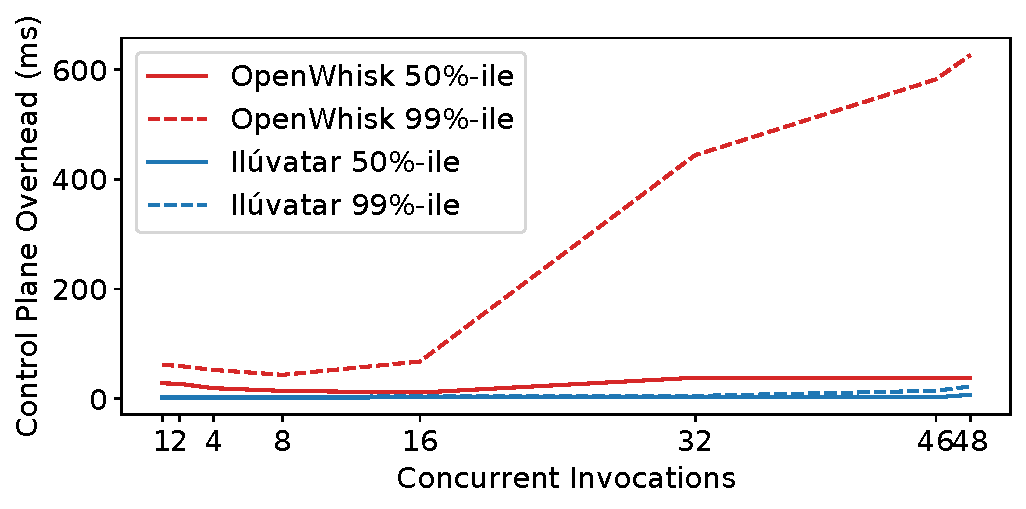
\includegraphics[width=0.4\textwidth]{iluvatar/graphs/scaling/pyaes/overhead-scaling.pdf}
  \caption{The latency overhead of the control plane, as the number of concurrent invocations increases. 
        OpenWhisk overhead is significant and has high variance, resulting in high tail latency. 
        \sysname~ reduces this overhead by 100x. }
  \label{fig:ow-scaling}
\end{figure}


\noindent \textbf{Performance.}
%
Because of its central role in coordinating all aspects of function execution, the control plane plays a major role in determining function performance. 
Managing the function execution lifecycle for hundreds of concurrent invocations imposes a \emph{control plane overhead}, and increases the end-to-end latency.
This control plane overhead can be significant, and affects \emph{all} function invocations, including and especially the ``warm starts''. 
%Time spent in the control plane is simply measured by subtracting the execution time of the function code from the overall end-to-end latency.
This overhead (end-to-end latency minus the function code execution time) for the PyAES function from FunctionBench~\cite{kim2019functionbench} is shown in Figure~\ref{fig:ow-scaling}. 

The figure shows the 50 and 99 percentile overheads as the number of concurrent invocations are increased.
In each case, we are invoking the function repeatedly in a closed-loop, and concurrent invocations are achieved by using multiple client threads.
All invocations are warm starts.
The experiment is run on a 48 core server (more details in Section~\ref{sec:eval}), and the figure thus shows the performance at low and medium load conditions. 

From Figure~\ref{fig:ow-scaling}, we can see that the OpenWhisk latency overhead is more than 10ms,  which is already a significant increase in latency for small functions which dominate real-world FaaS workloads.
Worryingly, the 99 percentile overhead is much higher, and rises to as much as 600ms.
We also see strange inversions in the scaling behavior: the overhead reduces for certain load-levels, and then increases again.
This high overhead, high variance, and uncertain scaling behavior, results in many challenges for FaaS \emph{providers}. 
Due to these issues, low-latency functions see severe performance degradation, and resource provisioning and capacity planning becomes harder due to the high variance and performance unpredictability. 
%

Some of these latency overheads are an artifact of the architecture. 
The shared Kafka function queue can be a major bottleneck; and there are no explicit backpressure or load regulation mechanisms, which is compounded by the CPU overcommitment. 
%
For the sake of comparison, the figure also shows the latency overhead of \sysname~ in the same environment. 
We are able to achieve a per-invocation mean overhead of less than 2ms for almost all the load conditions.
Importantly, the tail overhead is also small: less than 3ms for less than 32 concurrent invocations, rising to 10ms when the system is saturated.


To emphasize, for a median function in the Azure workload which runs for 500 ms, OpenWhisk can increase its latency by 100\%.  
Thus, the control plane plays a crucial role in function performance.
We note that these are the best-case warm-start latencies, when the function's containers is fully initialized and in memory. 
Since function cold-starts impose such a major performance penalty (increasing latency by more than $10\times$), mitigating them has been a major research focus. 
However, because of temporal and spatial locality of access, caching and prefetching techniques can be extremely effective, and the cold-start rate is often less than $1\% $ of all invocations~\cite{faascache-asplos21}. 
The majority of invocations are thus ``warm'', where the performance is dominated by control plane overheads.
%\emph{We thus need a low-latency, low-jitter control plane.}

\noindent \textbf{System Design.}
%
As evidenced by the OpenWhisk architecture presented earlier, FaaS control planes are large, complex distributed systems.
Due to the continually evolving needs of FaaS applications and emergence of new sandboxing techniques (such as lightweight VMs like Firecracker~\cite{firecracker-nsdi20}), they are sandwiched between the scale and heterogeneity of FaaS workloads on one hand, and the deep stack of OS and virtualization components on the other. 

For instance, systems for running web services or microservices do not have to deal with large and highly variable sandbox management overheads, nor with highly heterogeneous request sizes.
For reducing tail latency, these systems can often rely on the OS CPU scheduler for processor sharing, can do CPU allocation at very fine granularity~\cite{kaffes2019shinjuku}, use queuing theory techniques~\cite{prekas2017zygos}, etc. 
At the other extreme, for longer running containers and VMs, their control planes, like OpenStack or Kubernetes face a much lower rate of VM arrivals and departures. and can do careful and ``hard'' resource allocation using bin-packing~\cite{cortez2017resource}.


Functions are highly heterogeneous, and can be seen as both latency-sensitive web requests \emph{and} large containers requiring significant system resources for several seconds. 
FaaS control planes thus have to do \emph{both} low-latency allocation \emph{and} pack CPU and memory resources on their servers carefully to maintain high system utilization.
%
%We posit that these competing needs present new challenges in large-scale distributed resource allocation.
Thus FaaS control planes are one of the more perfect microcosms of challenges in resource management and control in large scale distributed computing. 

A clean-slate control plane design helps us investigate the fundamental performance tradeoffs and challenges in this fast-evolving ecosystem.
Our new implementation also helps to identify the current performance bottlenecks and new avenues of OS optimizations. 


\noindent \textbf{Platform for Experimental Systems Research.}
%
Performance-focused FaaS research is already challenging due to the extreme scale and heterogeneity of the workloads.
These challenges are compounded by existing control planes like OpenWhisk that are unfortunately highly unpredictable.
The control plane jitter and the extreme bimodal cold vs. warm latencies makes it difficult to do reliable and reproducible research~\cite{mytkowicz2009producing}, and subtle environmental and configuration effects can mask the true effects of new research optimizations.
However, it continues to be a key component in developing and evaluating FaaS research~\cite{akkus_sand_2018, shahrad_serverless_2020, faascache-asplos21, faaslb-hpdc22, zhou2022aquatope, ensure-faas-acsos20, alzayat_groundhog_2022}. 
%OpenWhisk is a popular framework which has been used as a platform for investigating and optimizing many facets of FaaS execution.
With OpenWhisk, function performance can be severely affected by a myriad of configuration options, such as insufficient memory for CouchDB, networking configuration, Docker configuration, etc. 

Given the importance of the control plane, we want \emph{predictable} performance to a large degree. 
In our experience, research in FaaS is often hindered by the large overheads and complexity of existing control planes. 
Thus, \sysname~ is designed from the ground-up to be lightweight and provide predictable performance under different conditions. 
Our system implementation can potentially accelerate the development of new optimizations, clarify  our understanding of performance characteristics of this relatively new stack, and provide a platform for robust experiments. 
% Establishing a shared open platform enables easy comparison between research work
With a robust platform, the community can share knowledge and advances, while being able to compare against a well-known and trusted baseline.


\section{\sysname~Design}
\label{sec:design}

% Design goals:
%   A research control plane
%     Easy to use, adjust source code, modification points
%     Full system stack: controller (load balancer), worker(s), load generation, containers, workloads, simulation
%     Configurable, lots of knobs to adjust things easily
%     Tracking of metrics/resources/system events
%   low-variance! and low(ish)-overhead control plane
%   No frivilous features, not too complicated

\sysname's design is guided by our experience of OpenWhisk performance, and by our goals of providing predictable performance, modularity, and a control plane for reliable FaaS research.

% \vspace*{-8pt}
\subsection{Architecture and Overview}
\label{sec:design:arch}

The \sysname~control plane is spread out across a load balancer and the individual workers, and sits above the containerization layers. 
We intend for \sysname~to be the narrow waist~\cite{popa_http_2010} in the FaaS ecosystem: with optimizations for DAG scheduling~\cite{zhou_qos-aware_2022}, state handling~\cite{sreekanti2020cloudburst}, and horizontal scaling~\cite{faaslb-hpdc22} implemented above it, and sandboxing and containerization below it.  
This architecture was motivated by the key question: \emph{Can fast FaaS control planes be implemented with strict layering and separation of concerns?}


We have found that most of the control plane overhead is in the workers, and hence optimizing the worker performance is our major focus.
%
Our architecture is \textbf{worker-centric}, and places more performance and load-management responsibility on the individual workers, instead of a more ``top-down'' centralized approach favored by prior work such as Atoll~\cite{singhvi2021atoll} and others~\cite{kaffes_centralized_2019, kaffes_hermod_2022}.
Top-down resource management requires a consistent global view of the cluster, and is complementary to our work. 
Predictive techniques for load-balancing, prefetching, scheduling, function-sizing can all be effective, but we want to explore the performance characteristics and limits of \emph{reactive} control planes that work with unmodified container runtimes. 

\begin{figure}
  \centering 
  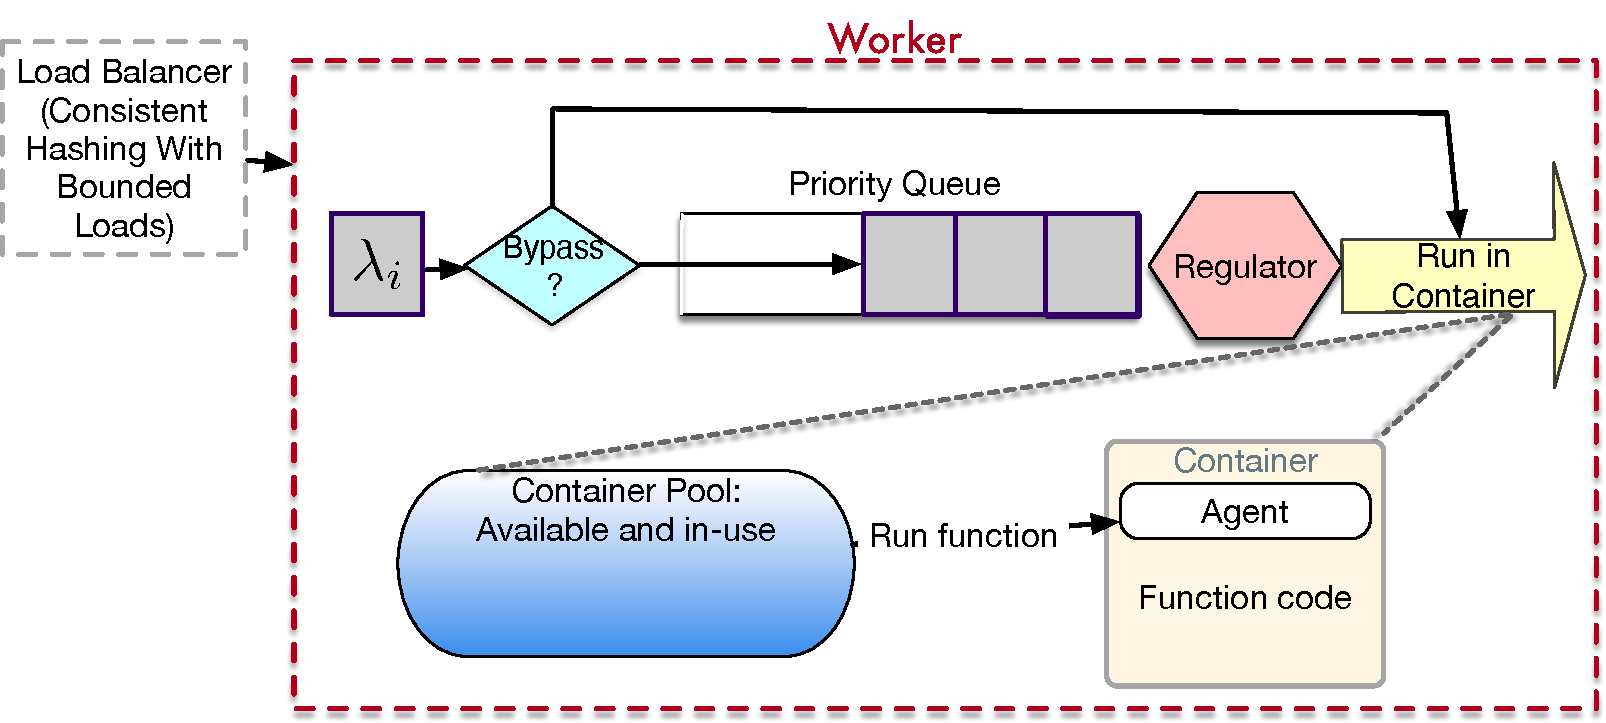
\includegraphics[width=0.95\textwidth]{iluvatar/figs/il76-q.pdf}
    % \vspace*{-6pt}
  \caption{\sysname~has a worker-centric architecture. A per-worker queue helps schedule functions, and regulate load and overcommitment. }
  \label{fig:arch}
  % \vspace*{-6pt}
\end{figure}

\sysname's main components are shown in Figure~\ref{fig:arch}.
Clients/users invoke functions using an HTTP or RPC API, with the main operations being \texttt{register, invoke, async\_invoke, and prewarm}.
Workers also provide load and status information to the load-balancer. 
We use stateless load-balancing, by using variants of consistent hashing with bounded loads (CH-BL), which have been proposed for FaaS recently~\cite{faaslb-hpdc22}. 
This is a locality-aware scheme, which runs functions on the same servers to maximize warm starts, and forwards them to other servers only when the server's load exceeds some pre-specified load-bound.


Continuing on the worker-centric theme, the worker API is a subset and almost completely identical to the overall API, and functions can be launched directly on a worker for single-worker setups and benchmarking, without going through a load-balancer and adding unnecessary latency.
The workers implement various latency-hiding and burst-mitigation techniques. 
All functions are launched inside containers, and dealing with the container layer is a major part of the worker. 
Each worker maintains a container pool of initialized containers for facilitating warm starts, and has an invocation queue for handling dynamic loads.
Function characteristics such as their cold and warm execution times are captured in various data-structures and are made available using APIs for developing data-driven resource management policies.

An important contribution and component of \sysname~is its principled support for function overcommitment based on its queuing architecture.
In many environments, like public FaaS providers, function resources cannot be overcommitted. 
However, the actual function resource usage is often significantly less compared to their requested \quotes{size}.
This difference is the motivation behind recent \quotes{right sizing} work~\cite{akhtar_cose_2020, guo_decomposing_2022, tian_owl_2022, eismann2021sizeless, kotni2021faastlane}, and can significantly improve system utilization.
Through its queue-based architecture, \sysname~supports a wide range of overcommitment scenarios, including no overcommitment, which is absent from OpenWhisk.
By default, OpenWhisk does not overcommit memory, but can  overcommit CPUs, which introduces performance interference and potential SLA violations for functions. 



%%%%%%%%%%%%%%%%%%%%%%%%%%%%%%%%%%%%%%%%


% \subsection{Function handling in the workers}
% \vspace*{-8pt}
\subsection{Function Lifecycle}
\label{sec:design:lifecycle}

%Function lifecycle is controlled by three main \sysname~worker API calls.
New functions first must be \emph{registered}, which entails downloading and preparing its container disk image.
The container images are fetched from DockerHub or some other image repository.
Container images are composed of multiple copy-on-write layers, and we prepare the images by selecting the relevant layers for the operating system and CPU architecture.
The images consist of the user-provided function code and our agent, which is a simple Python HTTP server that runs in each container. 
%How functions are registered and prepared to run by the control plane isn't immediately interesting research-wise, so we choose to do these out-of-band.
%
Registered functions can then be directly \emph{invoked}, which triggers launching of the function's container.
The first invocation is usually a cold start, which entails launching the container image from disk, or from a previous snapshot~\cite{ustiugov2021benchmarking, ao2022faasnap} if available. 
Each function container starts the agent which listens for and controls the actual function code execution. 
The agent has two simple commands, a \texttt{GET /} endpoint for simple status checking, and a \texttt{POST /invoke} to run an invocation with some arguments.
When the container is ready, the worker sends an HTTP request to the agent to start the function code execution. 
We detect the container's readiness using an inotify callback, which is a faster and more generic mechanism for notification compared to Docker's built-in API. 
%
Finally, when the function finishes execution, the HTTP call to the container's agent returns, and the container is marked as \quotes{available} in the container pool, to be potentially used for future invocations of the same function.

\begin{comment}
In the spirit of a fast \quotes{baseline} control plane and for isolation, \sysname~does not share containers across functions.
This is in contrast to SAND's application sandboxing~\cite{akkus_sand_2018}, SOCK's Zygote containers~\cite{oakes_sock_2018}, Nightcore~\cite{jia2021nightcore}, and even OpenFaaS~\cite{openfaas}.
%For example, recently proposed optimizations such as SAND's application sandboxing~\cite{akkus_sand_2018}, or SOCK's Zygote containers~\cite{oakes_sock_2018} share containers for concurrently running functions. 
% allow for functions to share a language runtime inside a container, or the same function to reuse 
% SAND's application sandboxing~\cite{akkus_sand_2018}, or SOCK's Zygote containers~\cite{oakes_sock_2018}. 
%We don't allow concurrent invocations of the same function to run in the same container like OpenFaaS~\cite{openfaas} or nightcore~\cite{jia2021nightcore}.
Our isolation model is similar to the public cloud providers. 
\end{comment}

Additionally, \sysname~introduces a standard \texttt{prewarm}  API call, which starts the function's container and the agent inside of it, and adds it to the container pool.
This reduces most of the cold start overhead associated with the container.
Prewarming can both avoid a \quotes{thundering herd} of cold starts on worker startup, and be an optimization in which the control plane anticipates invocations and prepares containers for them. 
This allows for a systematic mechanism to implement various recently proposed predictive prewarm policies~\cite{roy2022icebreaker, shahrad_serverless_2020, silva_prebaking_2020}. 

%When a container is created, our agent is started up inside it.




\begin{figure}
\centering 
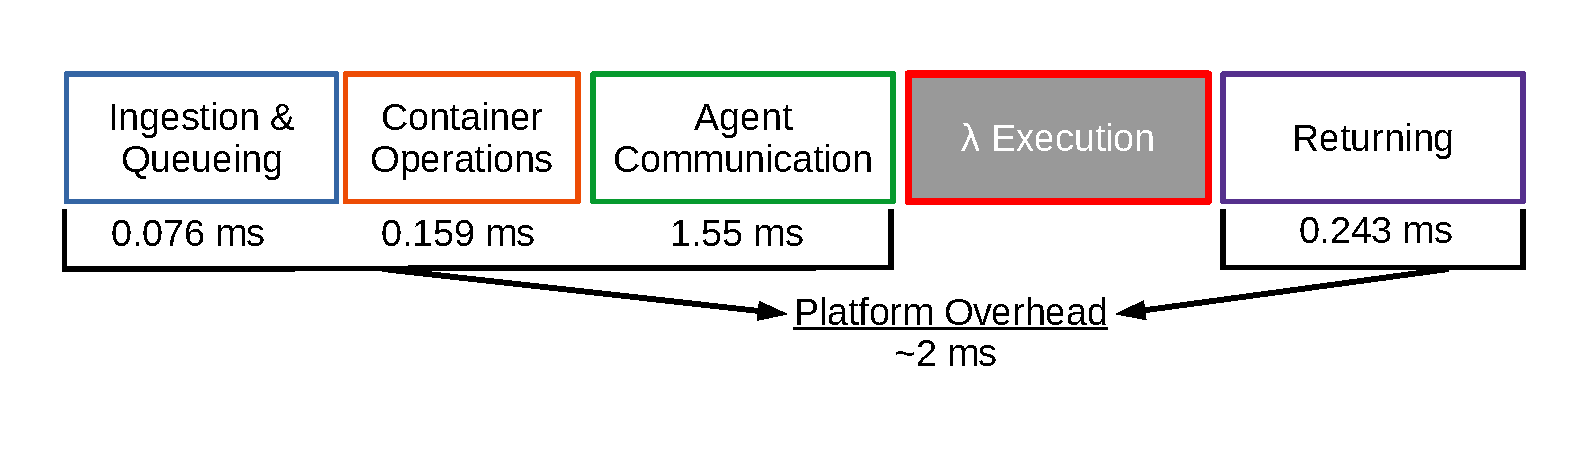
\includegraphics[width=0.95\textwidth]{iluvatar/figs/OverheadTimeline.pdf}
% \vspace*{-12pt}
\caption{The main components of the \sysname~overheads.}
\label{fig:timeline-flow}
  % \vspace*{\myfigspace}
  % \vspace*{-12pt}
\end{figure}


\noindent \textbf{Function Latency Breakdown.}
Throughout \sysname~and this chapter, we are interested in three main performance metrics. 
The first is the end-to-end latency of function execution, also called the \emph{flow time}, shown in Figure~\ref{fig:timeline-flow}.
This in turn has two main components: the control plane overhead is the latency of \sysname~operations, which are mainly before the start of function execution.
The second component is the function execution time, which is determined by the function code, and the load on the system.
The function execution time is our baseline, and we compute the \emph{normalized} end-to-end latency by dividing the full latency by the execution time (also called the \emph{stretch}). 

A more detailed latency breakdown is shown in Table~\ref{tab:overheads}.
The majority of overhead comes from the communication with the agent which is over HTTP. 
This is a deliberate choice, since we wanted to be compatible with existing OpenWhisk function images.
This can be reduced by using faster IPC mechanisms like in Nightcore~\cite{jia2021nightcore}. 
However, these faster communication approaches would reduce compatibility, especially with functions deployed inside VMs.

For OpenWhisk, a similar latency breakdown shows that a large amount of time is spent reading/writing to CouchDB (up to half a second), and the rest of the slowdown occurs in the Invoker (OpenWhisk's worker) and is primarily due to its design and implementation. 
Interestingly, the load-balancer/controller for OpenWhisk adds less than 3ms of latency even under heavy load, indicating that the worker-level performance is relatively more important. 
This further motivates our worker-centric design and evaluation focus. 


\begin{table}
  \centering 
  \caption{Latency of different \sysname~worker components for a single warm invocation.}
  \label{tab:overheads}
  \begin{tabular}{|c|c|r|}
    \hline
    Group & Function Name & Time (ms) \\
    \hline
    Ingestion \& Queuing & \begin{tabular}{@{}c@{}}invoke \\ sync\_invoke \\ enqueue\_invocation \\ add\_item\_to\_q \end{tabular} & \begin{tabular}{@{}c@{}}0.026 \\ 0.013 \\ 0.017 \\ 0.02 \end{tabular} \\
    \hline
    Container Operations & \begin{tabular}{@{}c@{}}spawn\_worker \\ dequeue \\ acquire\_container \\ try\_lock\_container \\ \end{tabular} & \begin{tabular}{@{}c@{}}0.029 \\ 0.02 \\ 0.096 \\ 0.014 \\ \end{tabular} \\
    \hline
    Agent Communication & \begin{tabular}{@{}c@{}}prepare\_invoke \\ call\_container \\ download\_result \\ \end{tabular} & \begin{tabular}{@{}c@{}}0.154 \\ 1.364 \\ 0.032 \\ \end{tabular} \\
    \hline
    Returning & \begin{tabular}{@{}c@{}}return\_container \\ return\_results \\ \end{tabular} & \begin{tabular}{@{}c@{}}0.017 \\ 0.266 \\ \end{tabular} \\
    \hline
  \end{tabular}
\end{table}

%As we can see, the overheads are minimal. Some queuing, some agent communication, which totals to about 3ms. 
% \vspace*{-8pt}
\subsection{Worker Performance Optimizations}
\label{sec:design:worker}

To achieve this low latency function execution for heterogeneous and bursty workloads, \sysname~uses two key underlying design principles: resource caching, and asynchronous handling of function life-cycle events.

\subsubsection{Resource Caching}

The cornerstone design goal of \sysname~is to reduce jitter, which we accomplish by removing expensive operations from the function's critical path. 
Instead, we cache and reuse as many function resources as possible, which minimizes the \quotes{hot path} function invocation latency significantly.
This principle is applied in various worker components, which we describe below.
A fast \textbf{Container Pool Keep-alive} and cached \textbf{HTTP Clients} allow for efficient warm start invocations.
Pre-allocating and caching \textbf{Network Namespaces} shortens cold starts---a technique first used for rapid container provisioning~\cite{oakes_sock_2018};

\noindent \textbf{Container Keep-alive.}
The primary and exemplary application of resource caching is in the container keep-alive cache that \sysname~workers maintain.
The containers become \quotes{warm} when their function has finished execution, and become \quotes{available} for the next invocation of the same function. 
We maintain a pool of all in-use and available containers for each registered function.
This container cache implements classic eviction policies such as Least Recently Used (LRU), and size-aware policies like Greedy-Dual-Size-Frequency, as proposed in FaasCache~\cite{faascache-asplos21}. 

\noindent \textbf{Network Namespace Caching.}
For isolation, each container is provided with a virtual network interface and a network namespace.
Through performance profiling, we've found that creating this network namespace can add significant latency to container cold starts---as much as 100ms.
This is due to contention on a single global lock shared across all network namespaces~\cite{oakes_sock_2018}. 
To minimze this overhead, we maintain a pool of pre-created network namespaces that are assigned during container creation. 
The isolation is still maintained, since concurrently running containers do not share the namespace. 
%Avoiding this expensive operation on the critical path.

\noindent \textbf{HTTP Clients.}
The worker threads communicate with the in-container agent for launching the function code.
Instead of creating a new HTTP client for every invocation, we cache a client per container and use connection pooling. 
This affects all invocations (even warm starts), and reduces the control-plane overhead latency by up to $3ms$. 

\subsubsection{Async Function Life-Cycle Handling}

The second key design principle is to handle various aspects of the function's lifecycle asynchronously off the critical path.
\sysname~achieves this through background worker threads for certain tasks, and through its Rust implementation which heavily uses asynchronous functions, futures, and callbacks wherever possible. 

\noindent \textbf{Keep-alive eviction.}
One such aspect is maintaining the function keep-alive cache, and ensuring that new functions have enough free memory to launch without waiting on existing containers to be evicted first.
Traditionally, eviction decisions would be made in an online fashion, but picking victims and waiting for their removal creates high variance in function execution times. 
\sysname~performs container eviction from the keep-alive pool  periodically in the background, off the critical path. 
This is similar to the Linux kernel page-cache implementation. 
We maintain a minimum free-memory buffer for dealing with invocation bursts, and periodically sort the containers list for eviction based on caching policies from~\cite{faascache-asplos21}. 

\noindent \textbf{Function Queuing.}
An important component of \sysname's architecture is a per-worker function queue.
New invocations are first put into the queue, and are dispatched to the container backend by a queue monitoring thread. 
%only when sufficient resources are available.
This allows us to tolerate bursts of invocations, and regulate the server load. 
% Details of our queuing policies are presented in Section~\ref{sec:q}.

%%%%%%%%%%%%%%%%%%%%%%%%%%%%%%
% \vspace*{-8pt}
\subsection{Container Handling}
\label{sec:design:ctr}

\sysname~uses standard Linux containers for isolating and sandboxing function execution---a \quotes{vanilla} and conventional approach.  
Several exciting new isolation mechanisms for cloud functions
have been proposed: such as lightweight VMs~\cite{firecracker-nsdi20}, unikernels, WASM~\cite{shillaker2020faasm} and other language runtimes~\cite{graalvm}, etc. 
Importantly, the sandboxing affects the \emph{cold start} overheads, which account for a tiny fraction of all invocations (usually less than 1\%).
Our control plane design and performance optimizations are independent of the sandboxing mechanism, and we address the orthogonal problem of optimizing the \emph{warm starts}. 

The basic container operations we use are: i) Create a container/sandbox with specified resource limits and disk image/snapshot, ii) launch a task inside it for the agent, and iii) destroy the container.
Each container is launched with the CPU and memory resource limits. CPU limits are enforced with cgroup quotas. 
This limited API allows \sysname~to support \emph{multiple} container backends.


By default, we use containerd~\cite{containerd}, which is popular container library, also used by Docker. 
The very rich containerization ecosystem presents a large number of options, and examining their tradeoffs was a major part of \sysname's design process.
Importantly, the choice of containerization library impacts the cold start times, and some library operations can take considerable time (100s of ms). 
High-level container frameworks like Docker are feature-rich and easy to use, but are typically used for long-running containers and are not optimized for latency.
Docker uses containerd under the hood, and it provides  more fine-grained control and slightly better latency.
Functions require a minimal containerization, and a lot of feature-complexity in these large containerization libraries can add to latency.
For instance, the crun~\cite{crun} library which is written in C takes about 150ms to launch a container, whereas containerd (written in Go) needs 300ms, and Docker needs 400ms. 

Using containerd allows us to use the OCI container specification~\cite{oci}, and makes it easier to support other container runtimes.
For instance, we also support the Docker container backend, which required only a minimal programming effort.
Containerd operates as a separate service, and we use it's RPC-based API, which contributes to some latency as well.
We contemplated writing our own optimized container runtime in Rust to avoid the overheads due to inter-process communication, extra process forks and system calls, and implement other cgroups and namespace optimizations. 
However, we ended up going with containerd to keep our control plane small and reusable across container runtimes.
We also wanted to investigate and tackle the challenge of getting predictable performance out of higher level containerization services that are not part of the same address space. 


\noindent \textbf{Simulation Backend.}
In addition to containerd and Docker containers, we also support a \quotes{null} container backend which is useful for simulations and evaluating control plane scalability.
%
Because of the scale and variety of FaaS workloads, using discrete event simulators for developing and evaluating resource management policies is often necessary.
%
For instance, the recent work on FaaS load balancing~\cite{faaslb-hpdc22} uses such a simulator for evaluating their policies at scale for different subsets of the Azure workload trace.
Usually, the simulation is used to augment and complement the \quotes{real} empirical evaluation of the same policies which are implemented in FaaS frameworks like OpenWhisk. 

However, a major methodological and practical issue is that the policy implementations, workload generation, and analysis, all need to be duplicated across the simulator and the real system.
This can lead to subtle and large divergences between the simulation and real environment. 
Moreover, the simulator cannot capture all the real-world dynamics and jitter, and can suffer from poor fidelity.

In order to aid researchers, \sysname~takes a different approach to simulations, and provides \emph{in-situ} simulations. 
Our \quotes{null} container backend does not run any actual function code, but instead sleeps for the function's anticipated execution time.
The rest of the control plane operates exactly as with real containers, and we still handle all other aspects of the function's lifecycle.
%
This allows us to simulate large systems and workloads. 
For evaluating any particular policy, researchers can use the simulator null-backend to evaluate control-plane overheads, warm-starts, etc., without requiring a large cluster.
Each \sysname~worker can \quotes{simulate} 100s of cores, since the CPU resources are only being consumed by the control plane, and not for running actual functions.
Alternatively, a large cluster can be simulated with multiple simulated workers. 

With this approach, \emph{there is minimal difference} between the simulation and the real system. 
Thus an experiment can be run in-situ or in-silico, following identical code paths.
The main distinction is that API calls to containerd are replaced with internal dummy function calls, and function invocations are converted to sleep statements.  
All control plane operations, control-flow, logging, resource limits enforcement, etc., are exactly the same as with the \quotes{real} \sysname.
This also helps with mocking and testing new policies. 

%%%%%%%%%%%%%%%%%%%%%%%%%


%%% Local Variables:
%%% mode: latex
%%% TeX-master: "paper"
%%% End:


\section{Function Invocation Queuing}
\label{sec:q}

As a way to regulate and control function execution and worker load, \sysname~ incorporates a per-worker invocation queue architecture. 
Function invocations go through this queuing system before reaching the container manager, which either locates the warm container and runs the function or creates a new container.
Each worker manages its own queue, differentiating our design from OpenWhisk's shared Kafka queue. 

\noindent \textbf{Motivation.}
%
This queuing architecture is motivated by three main factors: i) the bursty nature of the workload , and ii) Reducing cold starts due to concurrent invocations, and iii) to give workers additional mechanisms for controlling their load, implementing prioritization, etc. 
Note that once the function passes through the queue, it is effectively ``scheduled'' for execution by the OS CPU scheduler.
The CPU scheduler of course has its own throttling and controling mechanisms, such as cgroups and the various scheduler tuning knobs.
The invocation queue thus acts as a kind of a regulator or a filter before the CPU scheduler, and ideally, ``feeds'' it the right functions at the right rates for maximizing throughput and minimizing latency.
%

Because function workloads are so bursty and heterogeneous, running each function immediately can significantly increase the worker load and result in severe resource contention and increase  function tail latencies.
%
The queue also helps as an explicit back-pressure mechanism for load-balancing, admission control, and elastic scaling.
The queue length is  used for accurately determining the true load on the worker, which is a vital input to consistent hashing with bounded loads~\cite{faaslb-hpdc22}.
This reduces the staleness and noise of using system load average as the load indicator, and makes load balancing more robust.


Queuing invocations also allows us to reduce cold-starts.
While repeated function invocations are good and increase warm starts, 
\emph{concurrent} invocations of the same function results in cold-starts for all the concurrent invocations, since each invocation needs to be run in its own container.
This is also the ``spawn start''~\cite{ristov_colder_warmer}, which causes severe latency increase of 10s of  seconds in public FaaS. 
If there are $n$ concurrent invocations that arrive at the same time, then the $n$ concurrent cold-starts can significantly increase the system load and affect latency of other functions.
Instead, by queuing and throttling the functions, we can wait for the invocation to finish, and then use the warm container for the next function in this ``herd'', and so on and so forth. % Lol zizek 
%Having a queue allows us to regulate the invocations by this and other means. (?) 

% \vspace*{-8pt}
\subsection{Queue Architecture}
\label{sec:q:arch}

\sysname's queue architecture is shown in Figure~\ref{fig:arch}.
We have three main components.
%
From right to left, first, we have a concurrency regulator (or just regulator), which enforces the \textbf{concurrency limit}: the  upper-bound on the number of concurrently running functions. 
%
This lets functions execute \quotes{on cpu} without timesharing, and effectively determines the overcommitment ratio.
Higher concurrency limits (more than the number of CPUs) means  more CPU overcommitment.
Note that even with overcommitment, the cgroup quotas still provide proportional allocation (thus a 2 CPU container will still get twice the CPU cycles compared to a 1 CPU container). 
%
In addition to concurrency, other factors can also be used to regulate the queue discharge rate. 
The regulator can be used to run functions of only when sufficient resources (such as CPU bandwidth, warm containers, or even accelerators like GPUs) are available. 


%Note that technically the queue service backend is a processor sharing system, so can tolerate immediate execution albiet under heavy load.
%The concurrent cold start mitigation is one important component of the regulator policy.
%Its inputs are the number of currently running functions, the state of the container map to see which functions are executing, and the system resource utilization (load average, cpu\%, etc).
%This allows custom policies: we may want to limit the load average to under some limit, or the number of functions ``in flight'', etc.
\sysname~can be deployed with a fixed concurrency limit based on the usage requirements, or use its dynamic concurrency limit mode. 
In the dynamic mode, we use a simple TCP-like AIMD~\cite{yang2000general} policy which increases the concurrency limit until we hit congestion, which in our case is hit if the system load average increases above some specified threshold. 
Other metrics are possible: looking at the increase in execution time (i.e., stretch) of the functions could also be used as a congestion metric.
The concurrency limit affects the tail-latency, and more advanced policies can be implemented. 


\begin{comment}
Having the container map also allows us to implement \textbf{concurrent cold-start mitigation}.
If the function at the head of the queue has no warm containers available, and one of its instantiations is running, then we put the function back in the queue.
As a function's warm start is typically orders of magnitude shorter than cold starts, it is better for it to wait for warm container than to cold start one.
We implement this by asking the container pool for a warm container, and if it fails to give us one we can re-queue the invocation for the future.
Optionally, we can allow for a cold start to increase the number of warm containers for a function, naturally scaling if there is an increase in frequency.
\end{comment}

% This is currently implemented by looking at the container pool and estimating the likelihood of a warm vs. cold start, and using that expected execution time.
% The number of current concurrent executions are stored in the system statemap.


The second component is a \textbf{queuing discipline.} 
In the simplest case, we can use simple FCFS, and process functions in arrival order.
However, because functions are heterogeneous, this is not always the most appropriate.
Instead, we can use the past function execution characteristics such as their cold/warm running times for size-aware queuing such as shortest job first (SJF).
We elaborate more on the queuing policies in the next subsection. 

Finally, we note that queuing may increase the waiting time for small functions.
We thus have a \textbf{queue bypass} mechanism, which allows certain functions to bypass the queue and immediately and directly run on the CPU. 
Bypass policies take the function running time and the current system state as input. 
Currently, we implement a short-function bypass, where functions smaller than a certain duration are immediately scheduled, as long as the system is under a load-average limit.  
More effective bypass policies can also consider reinforcement learning approaches, since the action space is simple (bypass or enqueue), and the system state is well defined (functions running and in-queue, etc.).


% \vspace*{-8pt}
\subsection{Queuing Policies}
\label{sec:q:pol}

We implement multiple queue policies which leverage the repeated invocations of functions and use their learned execution characteristics to determining each function's priority.
To accomplish this, we maintain per-function characteristics such as cold time, warm time, and inter-arrival-time (IAT). 
%We maintain a sorted priority queue of invocations. 
We maintain a priority queue sorted by the function priorities, which are computed using their characteristics like arrival and execution time. 
%We can priority calculation to yeild differnt policy results.
%Different priority calculation yields different priorities. 

FIFO is simplest and invocations are just sorted by their arrival time.
For prioritizing small functions, we leverage our bypass mechanism, where the short functions can skip the queue and be scheduled directly on the CPU. 
Optimizing queuing policies for heterogeneous functions is challenging, and is an NP complete problem even in the offline case~\cite{bender1998flow}.


For improving throughput, we use shortest job first (SJF), which helps reduce the waiting time for short functions, but can lead to starvation for longer functions if the queue never drains. 
As a tradeoff between function duration and arrival, \sysname~ by default tries to minimize the ``effective deadline'' of a function, which is equal to the sum of its arrival time and (expected) execution time.
This earliest effective deadline first (EEDF) approach balances both short functions and starvation.
In both SJF and EEDF, an invocations' execution time is determined by its (moving window) warm time.
New/unseen functions have their times set to 0, to prioritize their execution.  
If we expect to find available containers for a function, we use its (moving window) warm time as the execution time in both SJF and EEDF.
Otherwise, we use its cold time---this also helps in reducing the concurrent cold starts, since the expected cold invocations of some functions in a burst separates them in the queue, and reduces the number of concurrently executing identical functions.
This spreading of function invocations over time increases the warm starts and overall performance. 
%
%Finally, we can  also prioritize functions with the highest inter-arrival-time. 
Finally, the RARE policy prioritizes the most unexpected functions (i.e., functions with the highest IAT). 

%All these policies can be combined with the short-function bypass technique.
%This also reduces the queue size and thus the overheads associated with maintaining a priority queue.
%In practice, the concurrency limit is larger than the number of the CPUs, so the queuing is expected to minimal under steady-state conditions. 


%L-p fairness:  $(\sum F^p)^{1/p}$


%%% Local Variables:
%%% mode: latex
%%% TeX-master: "paper"
%%% End:


\section{Implementation}
\label{sec:impl}

% Use a lot of provided stuff as a starting point
%   Containerd for isolation/container startup
%   CNI for networking
%   prebuilt Docker images
%   Rust language for efficient compiled language, without garbage collection interference
%   Tokio async handling & userspace threads

\sysname~ is implemented in Rust in about 13,000 lines of code.
It will be open-sourced upon paper acceptance. 
Its low latency and lack of jitter are attributable to the various low-level profile-guided performance optimizations we have implemented during the course of its development and testing.
Function handling and container management in the worker make up a majority of the implementation footprint and focus. 
Ours is a heavily asynchronous implementation using the \texttt{tokio} library in Rust, and various function lifecycle events spawn new userspace threads and trigger callbacks. 
The major data structure shared by the various worker threads is the container pool, which is implemented using the \texttt{dashmap} crate, which is a concurrent associative hashmap--- this provides noticeable latency improvements compared to a mutex or read-write lock.
Conversely, we still use a mutex for the queue, since we found minimal performance degradation compared to a no-queue architecture during profiling. 
These, and many other small optimizations, keep the \sysname~
resource consumption small: even under a heavy and sustained load that saturates a 48 CPU server, the worker process uses less than 20\% of a single CPU core. 




%%%%%%%%%%%%%%%%%%%%%%%%%%%%%%

%\noindent \textbf{Agent Optimization.}
%All our functions are written Python, and we do some Python-specific optimizations during their prewarm.
%The agent imports the function Python code, loading it and any library dependencies into memory, plus executing statements not in functinos, such as downloading an ML model.


% \paragraph{Deployment}
% For ease of repeatable and scalable use, we have set up our system to be deployable with Ansible \cite{}.
% In a command it can configure, set up, and tear down the applications that make up \sysname{}, and even capture artifacts like logs.
% It ties in nicely with the detailed configuration supported by our worker and controller services.
% Our services support configuration via a json file, convenient for development and local testing, but less so for large research experiments.
% Ansible, plus some clever config loading, allow us to inject arbitrary values as part of a larger command, making deployment for different experiments a breeze.

% With this setup, \sysname{} can be configured and deployed to any number of nodes with a single command.
% With this we easily scripted a variety of setups for our experiments in Section \ref{Evaluation}, giving us consistent and controlled environments and results.
% Workers are configured with a json file on startup, with the various policy options (such as queuing), keep-alive, timeouts, networking, logging, etc.

% CNI and container-spec are also provided as json files. For the container-spec, we change....

% Workers have four main services: Containers, invocation, network, and status.

% \vspace*{-8pt}
\subsection{Support for FaaS research}
\label{sec:impl:support}

One of our major design goals is for a reliable and extensible control plane for performance-focused FaaS research.
We now describe some of the \sysname~ features and our experiences in extending it.


\noindent \textbf{Performance Metrics.}
We keep track of all internal and external function metrics (such as their cold/warm execution time histories, inter arrival times, memory footprints, etc.) and provide them to all components of the control plane, and also to external services.
%
One of \sysname's implementation goals was to reduce the reliance on external services for system monitoring etc.
We thus track key system metrics like CPU usage, load averages, and even CPU performance counters and system energy usage using RAPL and external power meters.
These metrics are collected using async worker threads, and provide a single consistent view of the system performance.
%
Additionally, we also use and provide Rust-function tracing for fine-grained performance logging and analysis.
We use the \texttt{tracing} crate to instrument the passage of invocations through the control plane components, and obtain detailed function level timing information, which is used for identifying control plane and container-layer bottlenecks. 
%These logged details helped us with performance bottlenecks, but by default we keep disabled because it can increase per-invocation latency due to the overheads and CPU contention from creating so many logging events and it increases log file output size dramatically. 

\noindent \textbf{Adding New Policies and Backends.}
%
Using function and system metrics allows for easy development of data and statistical learning based resource management policies to be implemented.
Our baseline policy implementations for keep-alive eviction, queuing, load-balancing, are all easily extensible using Rust traits, polymorphism, and code generation. 
In our experience, adding new policies is relatively straight-forward, even for new-comers.
For example, all the priority-based queuing policies (SJF, EEDF, RARE, etc.) were implemented by extending the base FCFS policy.
Implementing and testing these policies took less than a few dozen lines and about four hours for a graduate student unfamiliar with the code-base. 

The default container runtime backend is \texttt{containerd}, but the interface is small, and supporting new backends is relatively easy.
We added Docker support in about 400 lines and one person-day of development effort.


\textbf{Load-generation and Testing.}
In the spirit of providing a full-featured system for FaaS experimentation, we have developed a load-generation framework.
It can do closed and open loop load generation, and be parameterized by the number and mixture of functions, their IAT distributions, etc. 
The testing framework can use functions from FaaS suites like FunctionBench~\cite{kim2019functionbench}, or custom sized functions that run lookbusy~\cite{lookbusy} for generating specific CPU and memory load.
%
The open-loop generation produces a timeseries of function invocations, which is helpful for repeatable experiments.
The functions' IAT distributions can be exponential, or be derived from empirical FaaS traces like the Azure trace~\cite{shahrad_serverless_2020}.


For the Azure trace, we start by randomly sampling functions and computing the CDF of their IATs.
We compute the expected load level in the system using Little's law, by finding the expected number of concurrent invocations for each function and adding them for all functions.
This expected load can be significantly different from the capabilities of the system under testing (for example, 100 concurrent functions will overload a 12 core system). 
Therefore, we can scale the individual function IAT CDFs to find a suitable load. This also allows us to change the relative popularities of individual functions, and conduct fine-grained sensitivity experimentation (like examining system performance when the popularity of one single function
changes, etc.).
We can generate larger traces by layering, and merging the traces from multiple smaller workloads.  


For synthetic functions (using lookbusy), we use their distribution of running times and memory consumption when generating the workload.
When using real functions from a benchmark-suite like FunctionBench, for each randomly sampled function, we use its average execution time (from the full trace), and assign it the closest function in the suite.
For example, if the average running time of a candidate function in the Azure trace is 8 seconds, we represent it using the ML-training function, which has the closest running time of 6 seconds.




%%%%%%%%%%%%%%%%%%%%%%%%%%%%%%


%%% Local Variables:
%%% mode: latex
%%% TeX-master: "paper"
%%% End:


\section{Experimental Evaluation}
\label{sec:ilu:eval}
We have extensively tested \sysname's performance characteristics throughout its development.
Here, we present a limited set of its key performance attributes and focus on new insights into FaaS performance.
All our experiments are conducted on a 48 core Intel Xeon platinum 8160 CPU, and we restrict the worker to 32 GB memory, running Ubuntu 20.04 using Rust version 1.67.0 and Tokio library version 1.19.2.
%
We are interested in evaluating latency overheads and \sysname's suitability as a low-jitter research control plane. 
This evaluation focuses exclusively on the performance of the worker, where we think most per-invocation latency improvement opportunities exist.
Many effective load-balancing policies have been published, but their impact on latency is limited to balancing decision time and warm start ratio.
Our stateless controller's overhead is consistent at less than 0.5ms, and we can thus ignore its latency contribution, for ease of exposition.
Our CH-BL based load-balancer maximizes locality and provides 99\% warm starts, and we focus on single-worker performance to remove unnecessary confounding factors.

% \noindent \textbf{Load Generation.}
% To collect benchmarking data and testing Control Plane Overhead for the different functions we generate \emph{closed loop} requests with varying client threads for 30 min each. We calculate the average for normalization of data collected in any other experiment. 

% For testing different Queue Policies we use open loop request generation. 

% \noindent \textbf{System Tweaks.}
% Ilúvatar itself keeps track of the memory usage and can limit number of concurrent requests dispatched to the system. We use Linux CPU Hotplug support to turn off some of the CPU cores to limit the system size. 

% \vspace*{-8pt}
\subsection{Control Plane and Function Performance}
\label{sec:ilu:eval:ovhead}

\begin{figure}
  \centering  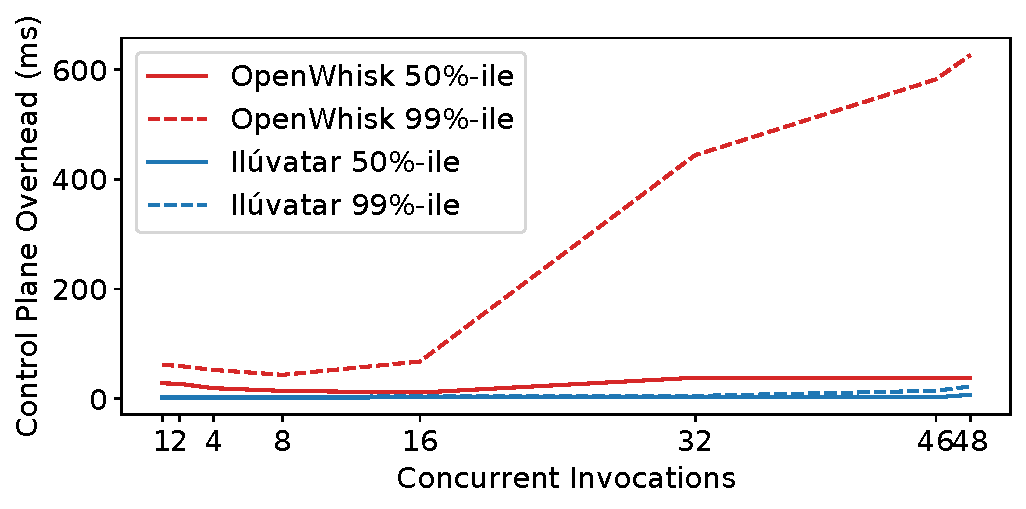
\includegraphics[width=0.6\textwidth]{iluvatar/graphs/scaling/pyaes/overhead-scaling.pdf}
  \caption{The latency overhead of the control plane, as the number of concurrent invocations increases. 
        OpenWhisk overhead is significant and has high variance, resulting in high tail latency. 
        \sysname~reduces this overhead by 100x. }
  \label{fig:ow-scaling}
\end{figure}

\begin{comment}
\begin{figure}
    % Results for pyaes, which has runtime of ~300 ms
    % [0.8, 0.9, 0.99, 0.999, 0.9999, 0.9999]
    % 1 [2.26 2.29 2.40 4.40 4.59 4.59]
    % 2 [2.19 2.24 2.32 3.97 4.74 4.74]
    % 4 [2.28 2.32 3.07 4.81 5.76 5.76]
    % 8 [2.27 2.31 2.48 4.84 12.16 12.16]
    % 16 [2.60 3.02 4.65 7.89 8.66 8.66]
    % 32 [3.18 3.36 4.97 7.91 10.71 10.71]
    % 46 [5.02 6.19 14.50 20.25 26.02 26.02]
    % 48 [12.31 14.89 22.25 28.86 32.52 32.52]
  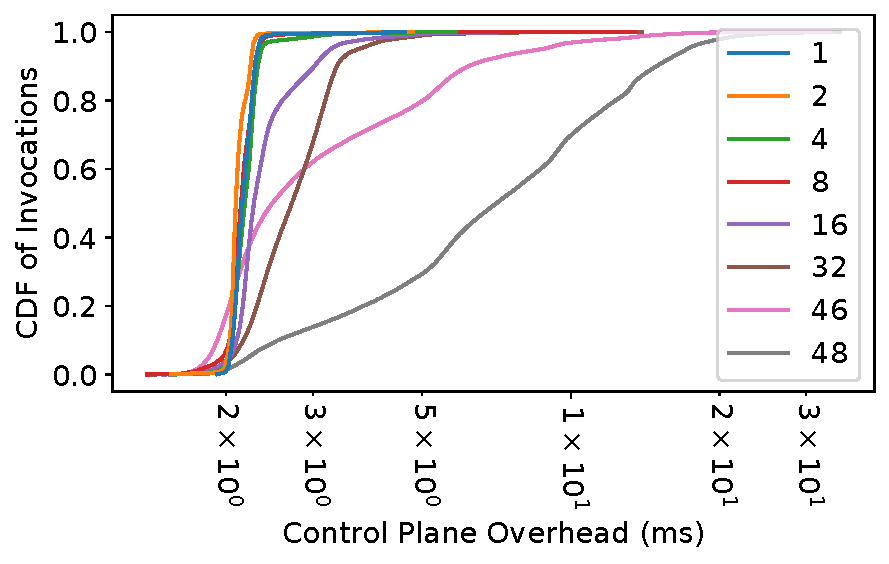
\includegraphics[width=0.6\textwidth]{iluvatar/graphs/scaling/pyaes/overhead-cdf.pdf}
    %  \vspace*{-6pt}
     \caption{\sysname~provides low latency overhead across a range of concurrent invocations.}
        % \vspace*{-6pt}
    \label{fig:ovh-cdf-aes}
\end{figure}
\end{comment}
% Results for lin_pack which has runtime of ~300 microseconds
% Percentiles: [0.8, 0.9, 0.99, 0.999, 0.9999, 0.9999]
% Thread count results (in milliseconds):
% 1 [2.69 3.01 5.68 940.41 956.48 956.48]
% 2 [2.69 2.94 7.12 940.17 942.17 942.17]
% 4 [2.16 2.53 5.74 928.90 935.37 935.37]
% 8 [2.00 2.35 4.78 833.26 860.58 860.58]
% 16 [3.13 3.70 7.05 664.69 709.56 709.56]
% 32 [6.30 7.54 13.78 351.35 430.77 430.77]
% 46 [9.62 11.83 20.14 103.92 15406.05 15406.05]
% 48 [9.64 12.14 20.85 73.48 31507.97 31507.97]

% Results for json_dumps_loads which has runtime of 0.5-1.5 seconds
% [0.8, 0.9, 0.99, 0.999, 0.9999, 0.9999]
% 1 [3.41 3.50 3.87 7.66 10.54 10.54]
% 2 [3.41 3.48 3.99 7.09 12.99 12.99]
% 4 [3.61 3.70 4.20 7.93 8.59 8.59]
% 8 [3.74 3.85 4.81 9.00 15.24 15.24]
% 16 [3.73 3.85 4.27 8.35 15.27 15.27]
% 32 [4.08 4.21 5.15 8.77 15.98 15.98]
% 46 [4.10 4.24 5.27 8.95 15.92 15.92]
% 48 [4.11 4.25 5.17 8.79 16.02 16.02]  

In this subsection, we focus on the latency overheads of \sysname~under different workloads and configurations.
For these experiments, we do not use any queuing, use a single worker, and focus on the most basic \sysname~configuration.  

We start by examining the control plane overheads under a closed-loop load for 30 minutes generated by different number of client threads. 
The control plane overhead CDF for the AES function is shown in Figure~\ref{fig:ow-scaling}. %~\ref{fig:ovh-cdf-aes} 
With 48 concurrent client threads, all the CPUs are fully utilized by function execution. 
Even in this saturated case, the 90 percentile overhead is less than 20ms. 
Just below this saturation limit, with 46 threads, the 90 percentile overhead drops to less than 10ms, and the average is less than 3ms. 

%%%%%%%%%%

\begin{figure*}
  \centering
  \subfloat[PyAES \label{fig:flow:pyaes}] {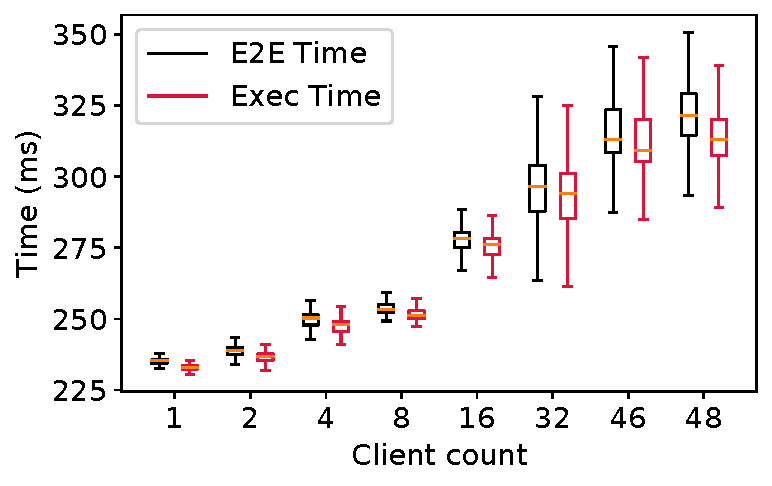
\includegraphics[width=0.3\textwidth]{iluvatar/graphs/scaling/pyaes/worker-e2e-and-exec.pdf}}
    \subfloat[JSON \label{fig:flow:json}] {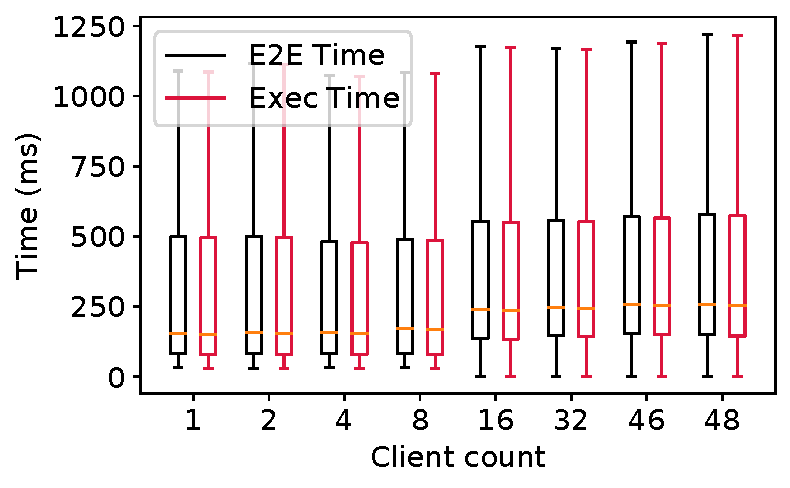
\includegraphics[width=0.3\textwidth]{iluvatar/graphs/scaling/json_dumps_loads/worker-e2e-and-exec.pdf}}
    \subfloat[Video \label{fig:flow:video}] {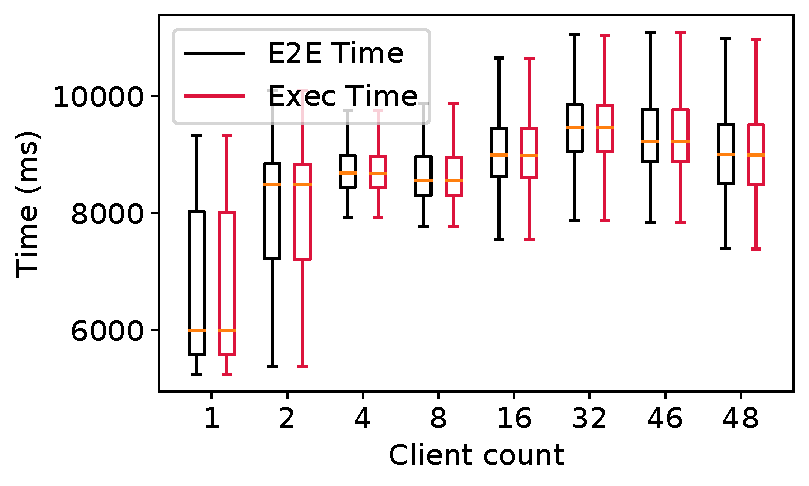
\includegraphics[width=0.3\textwidth]{iluvatar/graphs/scaling/video_processing/worker-e2e-and-exec.pdf}}
      %  \vspace*{-6pt}
      \caption{End-to-end latency and execution times for different functions as we increase the concurrency levels.}
        %  \vspace*{-6pt}
  \label{fig:flow-fn-all}
\end{figure*}

We now provide a more detailed breakdown of the function latency.  
In Figure~\ref{fig:flow-fn-all}, we look at the end to end (E2E) function latency (i.e., flow time) and execution time of different representative functions under different loads.
The flow time is impacted by the control plane overhead and the function code execution time. 
Both these factors are affected by the system load, which in turn is affected by the concurrency level.
% We vary the number of clients invoking the same code in a closed loop, and had each client register the code as a unique function with the system.
The difference between the E2E and the function execution time is the control plane overhead, which is small for all functions and at all load levels.


Interestingly, a significant source of latency variance is the function execution time itself. 
For the small, CPU-intensive PyAES function (Figure~\ref{fig:flow:pyaes}), the  inter-quartile-range is 60ms, which is 20\% the average execution time.
Both the execution time (and hence the E2E latency) and the variance also increases with the system load.
%
This variance is also determined by the non-determinism in the function code.
For instance, the JSON function (Figure~\ref{fig:flow:json}) parses a random json file on every invocation, and thus has a higher natural variance in its execution time.
%
Finally, the video processing function is long and CPU intensive: it downloads and converts a video to grayscale. 
This magnifies the CPU contention, and the function latency increases from 6 to 9 seconds under heavy load.
%


The notable increase in execution time for all three functions is a result of  high  CPU cache miss percentage and a reduction in the instructions per cycle (IPC).
%
We also observed poor cache locality with an increasing number of CPU cores. When the same workload was run on half the number of CPUs (by disabling the rest of the CPU cores), the cache miss percentage significantly dropped (by more than 50\%), along with a proportionate reduction in the latency variance.
%
This highlights and emphasizes the deeper architectural challenges of FaaS, which were also shown by~\cite{shahrad_architectural_2019}. 
%We leave the study of the cause of this effect for future work.

\noindent \textbf{Result:} \emph{\sysname~overheads are small even under heavy load. Function code non-determinism and system load have a higher impact on the function execution times. }


%%%%%%%%%%%%%%%%%%%%

\begin{figure}
  \centering
  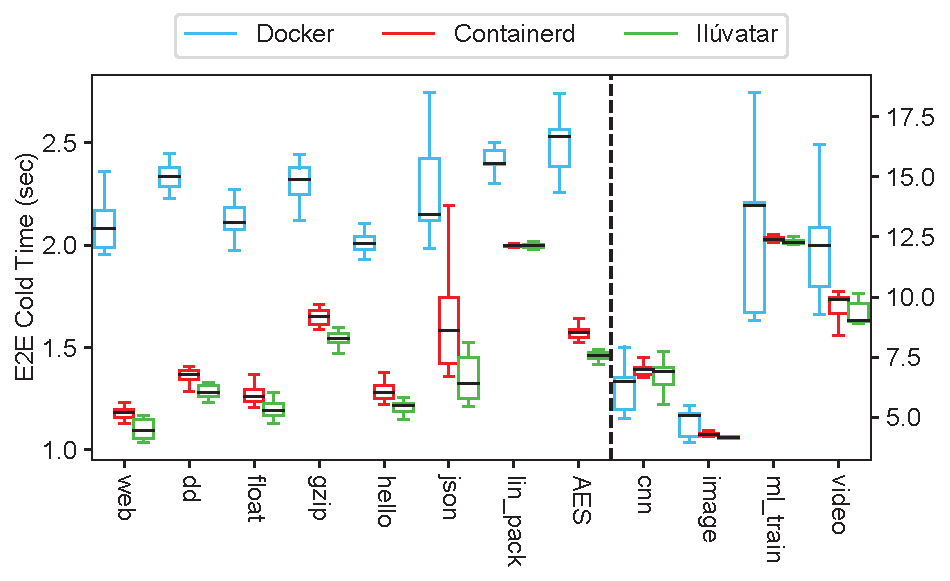
\includegraphics[width=0.6\textwidth]{iluvatar/graphs/impl/benchmark_cold_e2e.pdf}
  % \vspace*{-6pt}
  \caption{Most functions benefit from using a lower-level containerization and OS object caching on cold starts.}
  \label{fig:cold}
  % \vspace*{-6pt}  
\end{figure}

\noindent \textbf{Cold starts.}
So far, we have focused on warm-start performance which dominates function workloads.
\sysname~also incorporates a few optimizations for cold starts. 
Specifically, we are interested in quantifying the impact of the different container backends (containerd and Docker), and the network namespace caching optimizations. 
The end to end cold times for various functions are shown in Figure~\ref{fig:cold}: this includes both container startup time and function initialization overheads. 
In general, smaller functions face a larger impact due to the cold starts, since it represents a higher percentage of their total flow time. 


For small functions (left axis of the figure), using containerd (without network namespace caching) reduces the cold start by more than 40\%, indicating a clear advantage of using a lighter container runtime.
Introducing the namespace caching further reduces the cold start times by 15\% compared to unoptimized containerd which creates a new network namespace for each new container. 
After using the namespace cache, each function invocation sees upwards of $100 ms$ improvement in their cold start time.
%
The effects also hold for larger functions (right axis of Figure~\ref{fig:cold}), where Docker increases both the average and variance of the latency. 

% \vspace*{-8pt}
\subsection{Queuing Performance}
\label{sec:eval:q}

Having seen \sysname~performance in closed-loop micro-benchmarks, we now investigate the impact of its various queuing components and policies.
% We use our open-loop load-generation capabilities described in Section~\ref{sec:impl:support}.
We use an open-loop load-generator, with a random selection of 21 functions from the Azure traces, and pair them with different functions based on their closest running times.
This \quotes{stationary} workload has an average 40 requests per second for 30 minutes. 
This represents an extremely heterogeneous workload in terms of function durations and IATs.
Additionally, we also show results from a \quotes{bursty} workload generated in the same way, but with one function generating a burst of 18 requests per second for one minute.
In this open-loop testing, we prewarm the function containers to prevent excessive cold starts immediately at the start of the workload.
The number of containers to prewarm for each function is determined using Little's law by using their average rates and execution times. 

%~\ref{tab:workload-dsc} lists selected functions and theirs IATs. To test effectiveness of the queue policies we modify the baseline trace to include a burst of function invocation at the rate of 18 request per second in the middle of baseline trace for a window of one minute. Application dd in the table~\ref{tab:workload-dsc} represents it's IAT in bold.
\begin{comment}
\begin{figure}
    \begin{tabular}{|c|c|l|l|}
        \hline
        Application        & \begin{tabular}[c]{@{}l@{}}Benchmark\\ E2E Time (s)\end{tabular} & \begin{tabular}[c]{@{}l@{}}Baseline\\ IATs (s)\end{tabular}                                                       & \begin{tabular}[c]{@{}l@{}}Burst\\ IATs (s)\end{tabular} \\ \hline
        chameleon          & 0.0138       & \begin{tabular}[c]{@{}l@{}}0.076, 0.212, \\ 0.263, 0.391, \\ 0.398, 0.993, \\ 1.527, 3.292, \\ 4.381\end{tabular} & \begin{tabular}[c]{@{}l@{}}0.076, 0.212, \\ 0.263, 0.391, \\ 0.398, 0.993, \\ 1.527, 3.292, \\ 4.381\end{tabular} \\ \hline
        dd                 & 0.105        & \begin{tabular}[c]{@{}l@{}}0.213, 0.501, \\ 5.255, 5.944\end{tabular}                                             & \begin{tabular}[c]{@{}l@{}}\textbf{0.0547}, 0.213, \\ 0.501, 5.255,\\ 5.944,\end{tabular}                                  \\ \hline
        gzip\_compression  & 0.222        & 5.984                                                                                                             & 5.984                                                                                                             \\ \hline
        json\_dumps\_loads & 0.420        & 0.499                                                                                                             & 0.499                                                                                                             \\ \hline
        image\_processing  & 1.969        & 4.043                                                                                                             & 4.043                                                                                                             \\ \hline
        model\_training    & 5.974        & \begin{tabular}[c]{@{}l@{}}2.445, 3.004, \\ 3.746, 5.982, \\ 6.045\end{tabular}                                   & \begin{tabular}[c]{@{}l@{}}2.445, 3.004, \\ 3.746, 5.982, \\ 6.045\end{tabular}                                   \\ \hline
    \end{tabular}%
    \caption{Description of Workloads used for evaluation.}
    \label{tab:workload-dsc}
\end{figure}
\end{comment}

\begin{figure*}
  \centering
  \subfloat[Overcommit \label{fig:q-base:wted}] {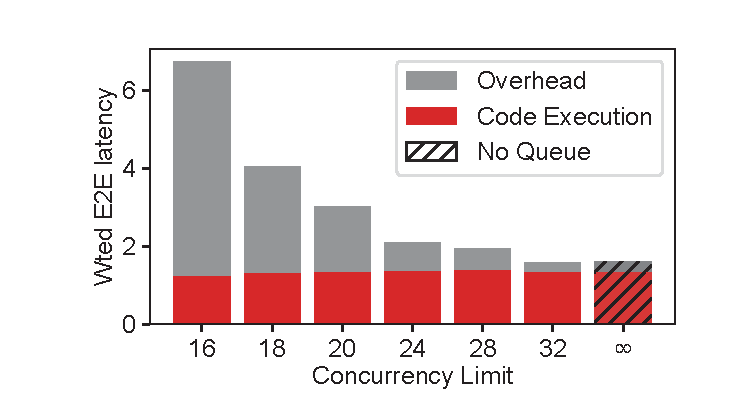
\includegraphics[width=0.6\textwidth]{iluvatar/graphs/old-baseline/breakdown/all_funcs_minheap_ed.pdf}}
  \hfill
  \subfloat[Distribution of function latencies \label{fig:q-base:box}] {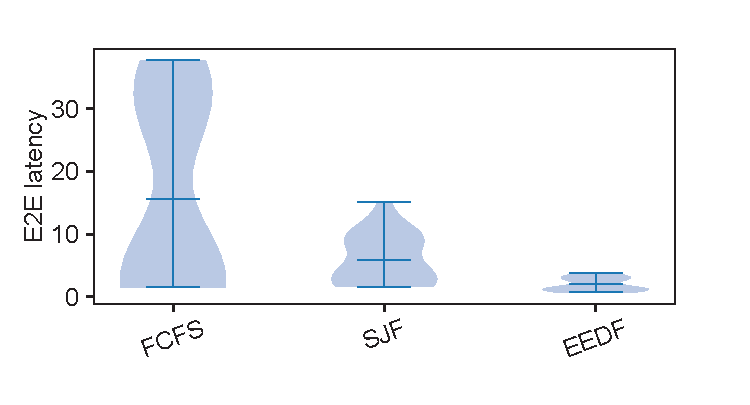
\includegraphics[width=0.6\textwidth]{iluvatar/graphs/scaled_trace2/trace_0_1/violin_e2e_for_each_queue/16_16.pdf}}
  \hfill
  \subfloat[Latency breakdown \label{fig:q-base:breakdown}] {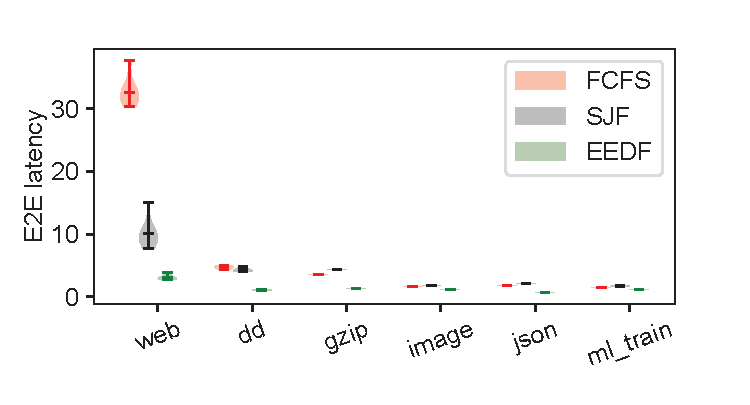
\includegraphics[width=0.6\textwidth]{iluvatar/graphs/scaled_trace2/trace_0_1/violin_func_breakdown/16_16.pdf}}
% \vspace*{-6pt}
  \caption{Queuing performance on the stationary Azure workload. Size-based policies can provide significant latency benefits.}
  \label{fig:q-baseline}
  %  \vspace*{-6pt}
\end{figure*}


\noindent \textbf{Metrics.} 
We use multiple performance metrics to understand and compare different policies.
Since functions can differ in execution time, we always normalize their total latency (flow time) by their execution time in an unloaded system. 
As shown in the previous figures~\ref{fig:flow-fn-all}, even with 1 closed-loop thread, the execution time has variance.
For normalization, we use the \emph{average} execution time with 1 thread for all the functions. 
Second, function popularities can also vary widely. 
We thus compute the \emph{weighted} latency, where each function's normalized latency is weighted by the number of its invocations in the trace.
Thus, the weighted latency represents the latency \emph{per-invocation}. 

\begin{figure}
  \centering 
  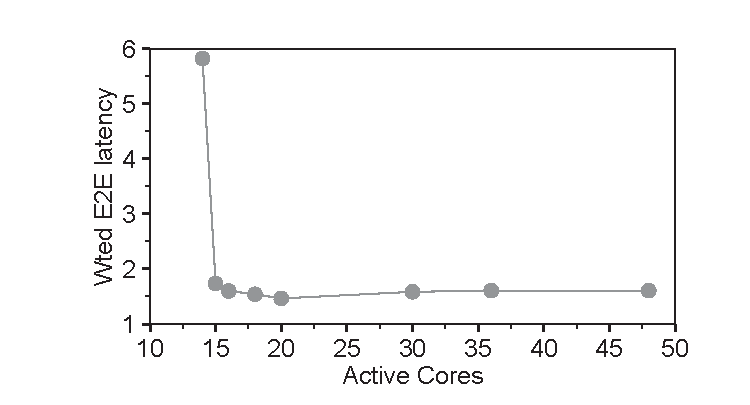
\includegraphics[width=0.6\textwidth]{iluvatar/graphs/scaling/WeakScaling.pdf}
    %  \vspace*{-6pt}
  \caption{The per-invocation function latencies for different system sizes (\# CPUs). We see a sharp inflection point at 16 CPUs, and use that in our queuing evaluation.}
    %  \vspace*{-6pt}
  \label{fig:weak}
\end{figure}


\noindent \textbf{Saturation Testing.}
We are primarily interested in how the queuing impacts the waiting time (which is part of the control plane overhead), and the function performance.
The analysis of queuing is interesting only in saturated scenarios, where there is enough extra load on the system and not all invocations can immediately run on the CPU.
We find this saturation point by weak scaling, and decreasing the number of CPU cores available to \sysname~(by disabling CPU cores using hot-unplug). 
The weighted and normalized latencies for different number of CPUs is shown in Figure~\ref{fig:weak}, which shows the performance \emph{without queuing.}
We see that for our baseline trace, increasing the number of available CPU cores has diminishing returns: the per-invocation latency doesnt benefit when CPUs are increased from 18 to 48.
However, we also see a sharp inflection point at 16 cores: decreasing the size to 14 cores results in a very high, almost $6\times$ slowdown. 
At 16 cores, our workload saturates the system, and we use this system configuration for all our queuing analysis.
We note that the alternative is to scale the workload up and run on on all 48 cores.
However, as we have shown previously through Figure~\ref{fig:flow-fn-all}, the poor hardware locality results in higher variance in the function execution times, and introduces more performance variance.
This variance often masks the control plane jitter, which is of more interest to us. 

% We evaluate our several queuing policies and compare them against a ``no-queue'' policy. 
% When there is no queue to limit concurrency, the control plane must either reject invocations when overloaded or allow resource overcommitment: namely processor sharing.
% Our system chooses the latter and will allow infinite invocations to run concurrently, so long as there is sufficient memory available, we do not overcommit memory.
% This behavior mimics how Openwhisk handles overload scenarios.
\begin{figure*}
  \centering
  \subfloat[Overcommit \label{fig:q-burst:wted}] {\includegraphics[width=0.6\textwidth]{iluvatar/graphs/scaled_burst_trace2/trace_0_1/barplot_breakdown_perqueue/all_funcs_minheap_ed.pdf}}
  \hfill
  \subfloat[Distribution of function latencies \label{fig:q-burst:box}] {\includegraphics[width=0.6\textwidth]{iluvatar/graphs/scaled_burst_trace2/trace_0_1/violin_e2e_for_each_queue/16_16.pdf}}
  \hfill
  \subfloat[Latency Breakdown \label{fig:q-burst:breakdown}] {\includegraphics[width=0.6\textwidth]{iluvatar/graphs/scaled_burst_trace2/trace_0_1/violin_func_breakdown/16_16.pdf}}
    %  \vspace*{-6pt}
  \caption{Small and bursty functions can get disproportionately impacted due to queuing. A little overcommitment can go a long way to reduce latency.}
    %  \vspace*{-6pt}
  \label{fig:q-burst}
\end{figure*}

\noindent \textbf{Impact of Overcommitment.}
Many frameworks like OpenWhisk inadvertently overcommit CPUs by running more functions than available CPU cores.
\sysname~can control the degree of overcommitment through its concurrency limit queue regulator.
Figure~\ref{fig:q-base:wted} shows the effect of this overcommitment, when the EEDF (earliest effective deadline) queue policy is used. 
The worker is limited to CPU cores, so higher concurrency limits represent different degrees of overcommitment. 
As the concurrency limit is increased, we see a reduction in the queuing time (which is a major part of the control plane overhead).
For instance, the queuing overhead is negligible when overcommitment level is 2 (i.e., 32 concurrency limit).
However we can see a tradeoff: the increased concurrency risks performance interference, and the code execution time also slightly increases (by 4\%).
For comparison and as a baseline, we also show the \quotes{no queue} configuration which is pure processor sharing and there is no limit on CPU overcommitment.
%
Queuing also reduces cold starts due to concurrent invocations. 
Without queuing, the number of cold starts increased by more than $3\times$. 

For the bursty workload, the impact of overcommitment is even more drastic, as shown in Figure~\ref{fig:q-burst:wted}.
A slight increase in concurrency limit can reduce the weighted latency by more than $3\times$, indicating that overcommitment is more effective for burstier workloads.
Interestingly, the latency improves by $20\%$ with queuing as compared to the \quotes{infinite overcommitment} no queuing case.
This is due to the increase in function execution time due to uncontrolled CPU contention and interference, which the queue helps ameliorate. 

\noindent \textbf{Result:} \emph{CPU overcommitment can reduce queuing times, but come with risk of increased performance interference. \sysname's queue design provides a new effective \quotes{knob} for managing this tradeoff.}

% Bursty here. 

\noindent \textbf{Queuing Policies and Fairness.}
Next, we look at the performance impact of the different queuing policies themselves.
We are interested in the impact on the latencies of the different functions. 
Figure~\ref{fig:q-base:box} shows the normalized latencies of different functions with the different queuing policies.
This scenario has a significant amount of queuing: the concurrency limit is set to 16 (the number of CPUs). 
The function-size aware policies like SJF and EEDF provide much lower latency compared to the standard FCFS: the average latency is reduced by more than $2-3\times$. % 30 to 10 
%The RARE policy prioritizes the highest inter arrival time, and is not size aware, and also tends to suffer under high loads.

A breakdown of the latency of individual functions in Figure~\ref{fig:q-base:breakdown} helps understand this stark performance difference.
The queuing in FCFS increases the total time of the extremely small \quotes{web} function (13ms running time), which increases its latency by $30\times$.
The small-function prioritization by SJF and EEDF reduces this significantly. 

The impact of queuing for the bursty workload is even more interesting, as shown in Figure~\ref{fig:q-burst:box}.
EEDF's average latency is $2\times$ higher than simple FCFS, while SJF is 60\% lower than FCFS. 
Investigating the per-function breakdown again in Figure~\ref{fig:q-burst:breakdown} again points to the contribution of the small web function, which is \emph{also the bursty function}.
The bursty invocations trigger the cold start mitigation, which deprioritizes them, and increases the queuing time, which disproportionately impacts the small functions.
% Bursty here. 

\noindent \textbf{Result:} \emph{Incorporating both function size and arrival times can improve function latency and fairness significantly. Very small functions see a higher \% increase due to queuing.}


%%%%%%%%%%%%%%%%%%%%%%%%%%%%%%


\noindent \textbf{\sysname~vs. Little's law vs. Simulation.}
Finally, we want to show \sysname's suitability for performance modeling, capacity planning, and as a research control plane for developing and evaluating FaaS resource management policies.
We compare the number of concurrent function invocations and queue length (EEDF) with the expected load according to Little's law, computed using average arrival rates and execution times of all functions of our stationary trace. 
We see that the real system metrics, even with all the inherent burstiness in the Azure trace, and the function execution and control plane jitter, are on average very close to the Little's law estimate.
This strongly indicates that our performance is indeed predictable even with highly heterogeneous workloads.

Additionally, Figure~\ref{fig:sim-vs-live-little} also shows the output of our ``simulation'' container backend described in Section~\ref{sec:design:ctr}.
This backend doesn't run actual function code, but exercises all other control plane aspects.
We use constant average function execution times (without accounting for variance and stochasticity) for all invocations.
Even though this simulation setup doesn't capture real-world variability and the impact of server load on function performance, we see that the simulation is also fairly closely aligned with the real experiment output.
This shows that \sysname's integrated simulation framework captures sufficient system dynamics and provides high-fidelity simulations.
This can significantly accelerate FaaS research, especially advances in reinforcement learning based scheduling, which requires high-quality simulations for learning policies. 

\begin{figure}
  \centering
  \includegraphics[width=0.6\textwidth]{iluvatar/graphs/trace-compare/baseline/minheap_ed/16/paper-status.pdf}
  \caption{\sysname~running in-silico closely models the in-situ performance. Making it a viable exploration opportunity supplementing real experiments.}
  \label{fig:sim-vs-live-little}
\end{figure}

% \subsection{Scalability}
% \label{sec:eval:scale}

% \textbf{Strong scaling. 48 worse than 16 because of ... bad locality?}

% \textbf{Simulation.}
% FaaS performance highly sensitive to workload due to skewed nature.
% Tough to experiment and report stable outcomes.
% For example, adding one function \emph{decreases} the overall latency. But its due to reporting.

% One way to avoid this is to look into simulations. Lightweight and allow different combinations to be thoroughly explored.

\begin{comment}
\noindent \textbf{Discussion.}
Our worker-centric design allows us to focus on single-worker performance. 
The load balancer is stateless and uses consistent hashing with bounded loads, and has a small overhead of less than 0.5 ms. 
Without workers sharing state (like with OpenWhisk's shared queue), there is no/minimal performance interference, and hotspots are confined in space and time.
%We conjecture that \sysname's performance improvements are largely due to the design and queuing policies for handling invocation bursts. 

Finally, our performance comparison with OpenWhisk is based on end-to-end latency testing. 
Performance tracing of OpenWhisk is challenging due to the highly distributed nature, and the drastically different architectures prevent a clean side-by-side comparison vs. the various components.
The use of Rust vs. Scala provides some performance gains as well, but all our OpenWhisk evaluation was conducted with ample heap sizes to reduce extra garbage collection overheads. 
\end{comment}

\begin{comment}
\begin{figure*}
  \centering
  \subfloat[Overcommit \label{fig:q-base:wted}] {\includegraphics[width=0.3\textwidth]{iluvatar/graphs/simulation/scaled_trace2/trace_0_1/barplot_breakdown_perqueue/all_funcs_minheap_ed.pdf}}
  \hfill
  \subfloat[Distribution of function latencies \label{fig:q-base:box}] {\includegraphics[width=0.3\textwidth]{iluvatar/graphs/simulation/scaled_trace2/trace_0_1/violin_e2e_for_each_queue/16_12.pdf}}
  \hfill
  \subfloat[Code Breakdown \label{fig:q-base:cold}] {\includegraphics[width=0.3\textwidth]{iluvatar/graphs/simulation/scaled_trace2/trace_0_1/violin_func_breakdown/16_12.pdf}}
 
  % \subfloat[Overcommit \label{fig:q-base:wted}] {\includegraphics[width=0.3\textwidth]{iluvatar/graphs/burst/breakdown/all_funcs_minheap_ed.pdf}}
  % \hfill
  % \subfloat[Fairness \label{fig:q-base:box}] {\includegraphics[width=0.3\textwidth]{iluvatar/graphs/burst/boxplot/16_24.pdf}}
  % \hfill
  % \subfloat[Cold \label{fig:q-base:cold}] {\includegraphics[width=0.3\textwidth]{iluvatar/graphs/burst/coldstarts/16_24.pdf}}
    % \vspace*{-6pt}
  \caption{Simulation baseline}
  \label{fig:q-burst}
    %  \vspace*{-6pt}
\end{figure*}
\end{comment}

%%% Local Variables:
%%% mode: latex
%%% TeX-master: "paper"
%%% End:


\section{Related Work}
\label{sec:related}

Alongside the closed-source FaaS control planes from the major cloud providers, a variety of other FaaS control planes exist.
Open-source production faas OpenWhisk~\cite{openwhisk}, OpenFaaS~\cite{openfaas}, nuclio~\cite{nuclio}, kNative~\cite{knative}, and funcX~\cite{funcx_hpdc_20}.
Others were made for with targeted research goals in mind~\cite{jia2021nightcore, hendrickson2016serverless, oakes_sock_2018, singhvi2021atoll,vhive-asplos21}.

\sysname~occupies a somewhat unique spot in the crowded FaaS landscape because of its focus on warm starts and some key constraints in our system design.
%
Techniques for reducing cold start overheads, like snapshots, language isolation,  unikernels, all sit ``below'' the control plane, and can be complemented with fast control planes.
At the other extreme end, the predictable nature of serverless workloads has been used to great effect for predictive load-balancing, prefetching, sizing, etc.
\sysname~is mostly reactive and is worker-centric, and tries to make minimal assumptions about workload predictability and focuses on more general optimizations that can work for arbitrary workload patterns.
%

\noindent \textbf{FaaS Control Planes.}
%
SOCK~\cite{oakes_sock_2018} is closely related to \sysname, and makes similar observations about network namespace overheads, and introduced storage and cgroup optimizations for serverless optimized containers. 
SOCK is based on OpenLambda~\cite{hendrickson2016serverless} and achieves great cold start performance with Zygotes that are cloned into new containers.
These optimizations to the container runtime are also applicable to \sysname~and are complementary. 
Using the standard containerd interface allows us to use multiple current and future container backends, and is a deliberate tradeoff. 
%Importantly it lacks both the ability to operate as a cluster and an integrated load generation system, both of which we have implemented both in \sysname~.


Nightcore~\cite{jia2021nightcore} is an integrated control plane and runtime system for low-latency microsecond-scale microservices.
It essentially implements containerized RPC, and uses fast message passing between the control plane and the agent.
Its special container runtime precludes generic ``black box'' functions, and it provides a weaker isolation model by running functions concurrently within the same container.
In the microservice context, container management and scheduling, dealing with heterogenenous functions, and other challenges are not relevant.


Atoll~\cite{singhvi2021atoll} is a fast and highly scalable control plane, and hugely benefits from pre-allocation and prediction.
It has a two level load-balancing setup with functions scheduled to a cluster group which then places them on a worker. 
\sysname's design and contributions are orthogonal to Atoll's more top-down and predictive approach, and we focus on the ``low-level'' worker problems.


Open-source control planes like OpenWhisk, OpenFaaS~\cite{openfaas}, nuclio~\cite{nuclio}, and kNative~\cite{knative}, are widely used to provide functions as a service. 
They tackle the competing demands of modularity and features, along with supporting function executions in generic environments.
Many FaaS systems use Kubernetes as the resource and container management layer, and its complexity and high latency further inhibits deep understanding and optimizations. 
OpenWhisk's cold and warm performance has been analyzed in many prior works such as~\cite{quevedo_evaluating_2019} and also as part of other systems~\cite{scheuner_lets_2022, alzayat_groundhog_2022, faaslb-hpdc22, faascache-asplos21}. 
OpenWhisk scheduling design and improvements can be found in ~\cite{kim_scheduling_2021, faaslb-hpdc22}.
Tighter latency requirements exist when deploying functions at the edge, and OpenWhisk's use on lower powered devices presents even more latency troubles~\cite{palade-edge-22, pfandzelter_tinyfaas_2020, hall_execution_2019, wang2021lass}. 
Interestingly, public cloud latencies are also significant, of the order of 50 ms~\cite{ustiugov_analyzing_2021}, hinting that the problems also extend their control planes. 
%All four of these control planes rely on Docker and Kubernetes for their deployment and scaling mechanisms.
%These existing tech stacks are highly useful, but limit the research possibilities of a platform, e.g. cold start optimizations and deploying to edge nodes become intractable.
%While \sysname~does have a Docker isolation implementation, it is to showcase the ability implement multiple containerization mechanisms and compare between them.


\noindent \textbf{Function Scheduling.}
Concurrent to our efforts, queuing of function invocations has been proposed in~\cite{zuk_call_2022}, which implements various size-aware policies like SJF. 
Surprisingly, and perhaps due to OpenWhisk overheads, their function slowdowns are extremely high: of more than $10,000\times$. 
An earlier theoretical queuing analysis of flow and stretch metrics is also presented in~\cite{zuk_scheduling_2020}. 
In contrast to \sysname's worker-centric design, a centralized core-level allocation design is presented in~\cite{kaffes_centralized_2019}.
In FaaS clusters, the tradeoffs in load balancing and early/late binding are evaluated in~\cite{kaffes_hermod_2022}.
Locality~\cite{faaslb-hpdc22}  and ML-based~\cite{yu2021faasrank} techniques for FaaS load-balancing take advantage of the high temporal locality and predictability of the FaaS workloads.
Our effort is more focused on reactive systems, and adding predictive allocation will only improve it. 

OS scheduler improvements can also improve FaaS workloads~\cite{fu2022sfs}. 
Regulating Linux CPU cgroups shares is also effective in overcommitment~\cite{ensure-faas-acsos20}.
Evaluating the effectiveness of these scheduling improvements when juxtaposed with queuing will be interesting. 
Scheduling function workflows and DAGs are a growing area~\cite{shen_defuse_2021,mahgoub_wisefuse_2022,zhou_qos-aware_2022}, and we focus on single-invocation optimizations. 

\begin{comment}
Restoring from snapshots~\cite{vhive, faasnap, catalyzer}


%The architectural implications are analyzed in~\cite{shahrad_architectural_2019}. We look at the higher levels of the stack, i.e., at the control plane. The paper identifies the fundamental factors affecting function performance at the hardware level due to cache misses, bad locality, etc. 
\paragraph{Edge.}
The lower resource availability of edge platforms also motivates lighter control planes. 
Tinyfaas is a apecialized FaaS platform for the edge 
\cite{pfandzelter_tinyfaas_2020}, but uses existing control planes like OpenWhisk and Kubless.
\cite{hall_execution_2019}


\paragraph{Scheduling.}

ANY papers that use previous running time/task size information!? Atoll. Aquatope. 

Tail latency: 50ms for warm-starts for the cloud.~\cite{ustiugov_analyzing_2021} 

RL scheduling~\cite{yu2021faasrank}. 

Lets trace it\cite{scheuner_lets_2022} , platform overheads etc.


Workflow and serverless DAG scheduling is complementary to \sysname. 

FnSched. Anshul~\cite{}. Centralized Scheduling? 

Sharing containers in SAND~\cite{akkus_sand_2018}

Hierarchical scheduling (within container) in HyperFaas. 

\paragraph{OpenWhisk.}
\cite{quevedo_evaluating_2019} evaluates the cold and warm times under OpenWhisk. 
OW Hash based scheduling described in~\cite{kim_scheduling_2021}.

Container sizing lot of attention, why! Uses OpenWhisk atleast\cite{guo_decomposing_2022}.
Also uses it and claims massive speedups.~\cite{kotni2021faastlane}

Aquatope\cite{zhou_qos-aware_2022} also uses prewarming for keepalive and is based on OpenWhisk.

%%%%%%%%%

Overcommittment: Owl~\cite{tian_owl_2022} also does interference.
So does ENSURE and fnsched. Overcommittment has impact on both the function execution time and control plane overhead (more functions to execute and more contention of cplane processes with functions.) We do overcommitment for only short functions with the bypass. Longer functions likely to be CPU intensive.


Our work: control plane sandwiched between isolation optimizations and data-driven overcommit and predictive. 

Completely orthogonal to optimal sizing like sizeless~\cite{}, OFC~\cite{}, COSE~\cite{akhtar_cose_2020},~\cite{guo_decomposing_2022}, etc.
\end{comment}


\sysname~a fast, modular, and extensible FaaS control plane made open source capable of running on heterogeneous and edge hardware. 
It is implemented in Rust in about 13,000 lines of code, and introduces only 3ms of latency overhead under a wide range of loads.
Its worker-centric architecture, resource caching based design, queue-based overcommitment and scheduling, and careful asynchronous implementation, all contribute to low latency and jitter. 
% \sysname~is open source, runs on heterogeneous and edge hardware, and is intended to serve as a platform for future high-performance FaaS research and deployments.
% In the near future, we intend to incorporate support for Firecracker~\cite{firecracker-nsdi20} VMs and GPUs; investigate load balancing optimizations; and deploy \sysname~on HPC and cloud clusters. 


% \chapter{Black-Box GPU Acceleration for Serverless}
\label{chap:gpu-sched}

% \section{Introduction}

Function as a Service (also called FaaS or serverless computing) is one of the fastest growing abstractions in cloud computing today with usage increasing by 2x in the past two years alone~\cite{wen2023rise}.
% Users create self-contained \textit{functions} whose lifecycle is orchestrated by the FaaS provider.  
Users are enticed by its dynamic scaling, low cost, and ease of management, as the lifecycle of self-contained \textit{functions} is orchestrated by the FaaS provider.
% Cloud providers benefit because functions use ephemeral resources unlike traditional virtual machines (VMs) and the provider has find-grained control over scheduling and placement.
Cloud providers leverage the ephemeral nature of functions into fine-grained control over scheduling, placement, and resource allocation.

% 1)
Current FaaS applications are limited by the capabilities exposed by providers, mostly consisting of short-running functions~\cite{shahrad2020serverless} using limited compute.
% Functions are given limited CPU resources and have no way efficient of coordinating with one another, precluding classic parallel computing.
Providers have not exposed GPUs or other parallel processing paradigms to their serverless platforms, a need for which is growing as users migrate new, intensive, workflows to cloud FaaS.
These applications see a \emph{minimum} 2.5x throughput improvement when accelerated, strong encouragement to enable such devices in serverless platforms.

% 2-3)
Accomplishing this transition requires the control plane to address several resource management problems.
Achieving high device utilization and low latency require device multiplexing~\cite{pemberton2022kernel, ng2023paella, fingler2022dgsf, gu2023fast}, but unmodified functions preclude such sharing of GPU resources.
% To make matters more complicated, GPU resources are managed by an esoteric device driver that isn't controllable by the OS.
Once a function is given access to the GPU, it can allocate the entire memory range or hog compute in a run-to-completion model.
% Idle periods mean allocated resources on the GPU are blocked off, other functions being unable to use them for their executions.
% Removing containers to release held resources results in heavy churn and increased latency from the repeated container initialization.
Swapping functions requires starting a new container, costing several seconds on the critical path, making the well-known \quotes{cold start} problem of FaaS an even larger latency bottleneck.
% We avoid cold starts by being the first to enable GPU keep-alive~\cite{faascache-asplos21} policies via GPU resource multiplexing.
Avoiding cold starts (i.e. a warm start) to get viable performance requires enabling GPU keep-alive~\cite{faascache-asplos21} policies via GPU resource multiplexing.

\begin{comment}
Machines used to host FaaS systems are expected to serve thousands of unique functions with low latency.
This is accomplished by running user function code inside a container (or VM), then keeping the container in memory but idle for future uses. 
A na\"ive adaption of this to the GPU problem would assign an entire GPU to each container for its lifetime.
Unfortunately an idle container then wastes GPU resources, and the limited number of GPUs per server leads to churn when we need to create a new container for another function.
% but this causes low utilization and high turnover when going to run a new function.
Virtualization for these devices exists, provisioning fixed slices of GPU resources to containers that they then have exclusive access to.
% This also results in low utilization, as nothing else can use that section when it is idle, and also limits the resources available to give to any one function that might take advantage of them.
While allowing more containers to exist concurrently, this solution does not address idleness and introduces a new limitation by reducing the maximum allocation any single function is allowed to make.
\end{comment}
  
% 4-6)
Multiplexed resources are not a performance panacea: the platform must now contend with function fairness and locality.
% The FaaS control plane must also guarantee that all functions will run in a timely and fair manner.
% GPUs must also be shared temporally 
Optimal performance is achieved by running one function repeatedly, as its data dependencies will be available on-device.
Yet a popular function can easily starve others of device time and violate fairness guarantees if not eventually blocked.
% Temporal GPU sharing between the highly heterogeneous serverless workloads must be balanced with execution \quotes{locality}.
New queuing policies tailored to the unique scenario of GPU-serverless computing must be designed to ensure fairness while maintaining high throughput.
% Warm hits, i.e. executing using an already existing container, have up to 100x lower latency compared to their cold counterparts.
% Such execution \quotes{locality} can only come 
% want warm starts.
% locality good -> 'batching'.
% but need spatial/temporal multiplexing as well.

% 7
Previous research work into enabling GPU acceleration in FaaS has focused on ML inference~\cite{pemberton2022kernel, ng2023paella, fingler2022dgsf, gu2023fast}; understandable given its popularity.
These approaches have abandoned the black-box nature of FaaS in favor of extremely fine-grained control of GPU usage and scheduling.
Supporting functions of all types is critical, as more use cases like scientific computing~\cite{kumanov2018serverless,hung2019rapid}, video encoding~\cite{ao2018sprocket, zhang2019video}, and optimization problems~\cite{aytekin2019harnessing,werner2018serverless,shankar2020serverless}, migrate to the platform.
% Our work uniquely enables all these to run natively with minimal overhead.
% Custom solutions have been proposed~\cite{}, but rely on targeted workloads or bespoke platforms, a general-purpose approach is needed.

% 7)
Given these known problems, in this work we seek to answer several research questions:
\begin{enumerate}[leftmargin=*]
  % \item Can we provide GPU acceleration to black-box, unmodified, serverless functions?
  % \item How can GPU support be integrated into high-performance FaaS control planes?
  \item Can we provide GPU acceleration to black-box, unmodified, serverless functions?
  \item Can we multiplex GPU resources between functions in a low overhead manner?
  \item How do we balance locality, fairness, and performance in the face of heterogeneous functions?
  % \item Is this possible without the cost of full virtualization?
\end{enumerate}
% \todo{Better RQs to frame novelty}

In this work, we propose and designed a series of techniques and policies that resolve all of these issues.
They enable black-box serverless functions to utilize GPUs for acceleration while concurrently sharing its resources.
We built our system on top of the \sysname~platform~\cite{fuerst2023iluvatar}, utilizing Nvidia's integration with Docker~\cite{docker-main}. %, but is generic to any accelerator or isolation system.
Importantly, they don't rely on specific hardware or software versioning support, and work on heterogeneous hardware regardless of age or capability. 

% \mhead{RQ1}
Starting from the lowest level component, we interpose an intercept shim between function code and the GPU driver.
Using this, we capture all memory allocation calls and transform them into Unified Virtual Memory (UVM)~\cite{nvidia-uvm} calls.
UVM memory allows applications to allocate beyond the device limits, letting the driver use host memory as swap space, migrating memory on demand. 
Once all allocations are converted to UVM memory, we use the shim to move memory between host and device under direction from the control plane.

% \mhead{RQ2}
Controlling memory positioning allows us to both oversubscribe device memory and keep containers warm while other functions execute on the GPU.
To enable multiple functions to run concurrently, a new queuing policy is required that better matches the new device's capabilities and workload characteristics.
We accomplish this with a modified implementation of a Mutli-Queue Fair Queue (MQFQ)~\cite{hedayati2019multi}, which prevents starvation, scales invocations across multiple GPUs, and minimizes execution overhead.
To prevent contention interference, we monitor device utilization using NVML~\cite{nvml} and track memory usage to throttle invocations.

With these controls we improve function latency by orders of magnitude over previous solutions and expand the pool of serverless applications.
In short, this work proposes the following enhancements to serverless computing:
\begin{enumerate}[leftmargin=*]
  \item We create a custom driver that intercepts function allocation calls to multiplex device memory.
  \item With no limit on device memory, we can keep idle containers resident, creating the first warm pool of GPU containers.
  \item Our memory management techniques allow us to reduce device pressure from idle functions, mitigating overcommitment overhead.
  \item We design a queuing policy that enables concurrent execution while ensuring fairness under heterogeneous workloads.
  % \item W
  % \item Benchmark suite of GPU-enabled serverless functions, including many non-machine learning applications.
\end{enumerate}

This paper is ordered as follows.
Section~\ref{sec:bg} covers background of serverless work and GPU virtualization.
Our motivation behind work is explained in detail in Section~\ref{sec:motiv}.
Section~\ref{sec:design} details our design of queuing, memory control, and resource management.
We examine the implementation of these pieces in Section~\ref{sec:impl}.
Lastly, Section~\ref{sec:eval} shows the effectiveness of our systems with a thorough experiment suite.
 

% \section{Why a new Serverless GPU Approach?}
\section{Serverless GPU Challenges}
\label{sec:motiv}

The current resources offered by serverless platforms severely limit the types of function workloads it can support.
% They are limited to a few GB of memory and limited vCPU time~\cite{lambda-limits}.
Memory is limited to a few GB and vCPU access is restricted to a single, time sliced, core~\cite{lambda-limits}.
Yet any function with a dataset that exceeds these limits or a problem space that needs parallel computing for timely results cannot be served.
% Moving computation to a GPU by providing faster solutions and increased device memory that is much more than current serverless limits.
GPU acceleration alleviates both of these bottlenecks and has the double benefit of improving existing workloads. 
We can't get this acceleration without cost unfortunately, several considerations need to be made for their benefits to shine.

\begin{comment}
\begin{table}
  \caption{Cold starts with a GPU can be worse because of container startup and library initialization. 
  If the execution is significant, this delay can still be a minor part of the latency.
  All times are in seconds.}
  \begin{tabular}{lrrr}
    \hline
    Function & GPU & CPU & GPU Speedup \\
    \hline
  FFT & 3.322 & 13.073 & 3.94x \\
  Ffmpeg & 4.612 & 34.260 & 7.43x \\
  Imagenet & 11.286 & 10.103 & 0.9x \\
  Roberta & 15.481 & 14.372 & 0.93x \\
  Eos & 4.904 & 1.049 & 0.22x \\
  Isoneural & 9.963 & 1.434 & 0.15x \\
  Lavamd & 2.136 & 14.161 & 6.64x \\
  Lud & 2.359 & 110.495 & 46.85x \\
  Myocyte & 4.339 & 39.662 & 9.15x \\
  Needle & 2.177 & 223.306 & 102.58x \\
  Pathfinder & 1.797 & 106.667 & 59.37x \\
  Srad & 3.945 & 123.499 & 31.31x \\
  Squeezenet & 6.793 & 4.672 & 0.69x \\
  RNN & 2.491 & 3.226 & 1.3x \\
  \end{tabular}
\end{table}
\end{comment}

\begin{table}
  \centering
  \caption{Attaching a GPU adds significant time to container startup overhead. All times are in seconds.}
  \label{tab:gpu-attatch}
  \begin{tabular}{lccc}
    \hline
    Function & GPU & No-GPU & Cold start Slowdown \\
    \hline
  Imagenet & 8.581 & 6.907 & 1.25x \\
  Roberta & 16.374 & 14.015 & 1.17x \\
  % Squeezenet & 5.809 & 3.966 & 1.47x \\
  % RNN & 4.284 & 3.776 & 1.14x \\
  Ffmpeg & 2.044 & 0.775 & 2.64x \\
  FFT & 2.648 & 3.677 & 0.73x \\
  % Eos & 2.408 & 1.589 & 1.52x \\
  Isoneural & 2.586 & 1.662 & 1.56x \\
  % Lavamd & 1.947 & 1.223 & 1.6x \\
  Lud & 2.125 & 0.736 & 2.89x \\
  Myocyte & 2.145 & 0.980 & 2.19x \\
  Needle & 2.292 & 1.453 & 1.58x \\
  Pathfinder & 1.997 & 1.029 & 1.95x \\
  % Srad & 2.213 & 3.313 & 0.67x \\
  \end{tabular}
\end{table}

\subsection{GPUs Containers}

\begin{comment}
GPU resources are not a free upgrade and must be treated differently from classical FaaS resource management.
Memory on a single device is limited to 10s of GB of memory compared to potential TBs supported by their hosts.
% To make matters worse, unmodified applications can allocate the entire device's memory range, preventing other functions from running without deleting the current one.
To make matters worse, an unmodified application can allocate the entire device's memory range, leaving the control plane with no recourse but removal to relieve pressure.
We cannot limit compute usage of a GPU as easily as one can use cgroups to limit a process' vCPU time.
Device compute kernels are arbitrarily sized, and are not guaranteed to be constant across function inputs.
Reducing the size of kernel launches (i.e. the number of threads it executes on) will increase execution time for the application and may cause crashes.
Launching multiple concurrent kernels which exceed the device's capabilities results in throttling, negatively affecting user latency.
% Function execution and container management must therefore
Ensuring memory and compute are available for function execution, while avoiding container churn, are critical for usable performance.
% Applications also tend to be contstrained by one of these two resources, as has been shown repeatedly~\cite{}, making co-locating challenging.
We use UVM tricks and monitor GPU compute to accomplish both of these tasks, without having to control individual kernel launches that many other systems use~\cite{pemberton2022kernel,gu2023fast,ng2023paella}.
\end{comment}

Serverless invocations are run inside isolated sandboxes, and creation of these typically happens on the critical execution path.
Such \quotes{cold starts} add significant latency to an invocation in comparison to actual function execution time.
Runtimes for functions are on the order of tens of milliseconds~\cite{shahrad2020serverless}, yet container startup may be several seconds: an order magnitude delay.

Creating a new container with an attached GPU is even more expensive.
Table~\ref{tab:gpu-attatch} compares the startup time for new Docker containers with and without a GPU.
Cold start times grow up to 3x, {adding an average of 1.5 seconds of latency} to an already costly process~\cite{du2020catalyzer,lin_mitigating_2019,manner_cold_2018,mohan_agile_2019}.
% Creating a new container with an attached GPU is also costly, Table~\ref{tab:gpu-attatch} compares the startup time for new Docker containers with and without a GPU.
We captured and broke down time spent starting a new ML inference container with and without an attached GPU in Figure~\ref{fig:cold-timeline}.
The bottom timeline with attachment has an additional second of startup from an Nvidia library hook performing kernel work.
% , even before counting time taken by the application for initializing the GPU and loading specialized libraries.
% has the accelerator and spends roughly 1.5 seconds in an Nvidia library hook that performs kernel work to attach the GPU to the container.
Once that is accomplished, the control plane agent starts loading user function code, which uses a more complicated startup procedure to prepare the device and allocate resources, taking an additional 1.5 seconds.
All serverless platforms use a warm-start pool of containers to amortize the cold start penalties across future invocations.
We created first such container pool for avoiding GPU cold starts using our memory multiplexing and manipulation techniques.
% These seconds exacerbate existing cold start overheads already seen~\cite{du2020catalyzer,lin_mitigating_2019,manner_cold_2018,mohan_agile_2019}, which are often longer than function execution time.
% All serverless platforms use a warm-start pool of containers amortize cold start penalties across subsequent invocations which GPU limitations have precluded.
% Our techniques provide the first warm-start pool of GPU containers in serverless to significantly improve latency.
% Without the ability to share a GPU resources, specifically memory, between several containers, this 
% The combination of limited memory for containers, plus high overhead times

\begin{figure}
  \includegraphics[width=\textwidth]{mqfq/graphs/coldstart/combined_timeline.pdf}
  \caption{Time spent in a cold start without (top) and with (bottom) a GPU attached to a container hosting TensorFlow inference code.
          % Several additional seconds are caused by Nvidia runtimes and user code library loading.
          GPU attachment adds over a second to initialization time, 
          and user code setup of the GPU increases agent startup inside the container. 
          }
    \label{fig:cold-timeline}
% Gunicorn & library load time, no GPU:
% gunicorn: 0:00:11.688722
% Gunicorn & library load time, GPU:
% gunicorn: 0:00:13.320342
% nvidia: 0:00:01.399233
\end{figure}

\subsection{Serverless Scheduling}

% The workloads in FaaS are unique challenge in cloud computing, and make getting good performance out of GPU acceleration a complex challenge.
The workloads in FaaS are highly heterogeneous and represent a unique orchestration challenge in cloud computing.
Memory usage, execution duration, and the inter-arrival-time between invocations can vary by several orders of magnitude~\cite{shahrad2020serverless}.


Previous GPU-enabling works do not address the potential for worker-level queuing of accelerated Serverless functions.
The first proposal~\cite{naranjo2020accelerated} used Docker and only shows performance improvement against CPU runtimes, neither queuing nor any drawbacks from switching computation are considered. 
Several examples~\cite{pemberton2022kernel,gu2023fast,ng2023paella} do schedule ML inference tasks and GPU resources for high GPU utilization, but do so by breaking apart each function to control kernel launches, thereby preclude whole classes of applications from running.

% Existing platforms avoid queuing, and if at all implemented use a simple policy such as FCFS (first-come-first-serve). 
Most scheduling serverless work targets cluster load balancing via locality~\cite{faaslb-hpdc22,kaffes_hermod_2022,abdi2023palette,package-cristina-19}, and avoid queuing at workers.
% A naïve queuing algorithm such as FCFS (first-come-first-serve) or Round Robin works well with CPU scheduling because it can rely on a large pool of containers.
If necessary they use First-Come-First-Serve (FCFS), which works well scheduling on CPUs because it can rely on a large pool of containers to avoid cold starts and expects little queuing of invocations.
Unfortunately, a FCFS policy neither take into account the need for fairness between functions under queuing, nor optimal use of limited device resources.
Moving data between host and device to change the running application is slow, as seen by~\cite{yu2019automatic, hong2017gpu} and we show below in Section~\ref{sec:shim}.
A new scheduling policy that considers locality of data on device and locality of functions in a smaller container warm pool are needed for viable GPU performance.
% Our memory multiplexing and manipulation
% However, the challenge of GPU locality and warm-pool leads these to high rates of cold starts, container churn, and loss of fairness.

% GPU functions also need data to be local

% Maintaining locality has seen much work~\cite{faaslb-hpdc22,kaffes_hermod_2022,abdi2023palette}, all trying to handle the highly heterogeneous~\cite{shahrad2020serverless} workloads of FaaS.
% Inter-arrival-times for functions can vary by several orders of magnitude, as do runtime characteristics such as execution time and memory usage.
% Inter-arrival-times for functions can vary by several orders of magnitude and are not fixed, complicating predicting when and how many containers will be needed.

% The CPU-GPU architecture differences require analyzing how FaaS keeps latency low, and determining how GPUs can fit in.
% Large host memory footprints are taken advantage of by FaaS to run the many containers needed to maintain high locality unpredictable functions.
% Limited GPU memory diminishes the chance for a local container warm hit, highlighting the need for a sizable container pool.
% Recently run functions will also benefit from architecture features like cache presence, and subsequent runs are less likely to need to pull external data dependencies.
% The large number of CPU cores on servers increases invocation concurrency

% A similar correlation exists with GPUs, they run faster when their data is \quotes{local} (i.e. on-device), as we show in our experiments in Section~\ref{sec:shim}.
% We resolve both problems with one solution: oversubscribe device resources and manipulate it for better locality.

% The limited resources of GPUs need a more advanced scheduler to provide \emph{locality}
% Our queue design can run invocations out-of-order, allowing several dispatches of a function in succession to increase warm hits, lowering latency.

GPU batching has been effective~\cite{ali_batch_2020,yang2022infless,ali2022optimizing} in improving GPU utilization and latency when executing ML tasks.
The inputs of multiple invocations are merged into one \emph{batch} by the control plane, computed together, and split apart to distribute results.
% Scientific applications among others are not amenable to batching, and for those that do, they require changing the FaaS paradigm.
Such white-box solutions eschew isolation by making assumptions about the workload, the fact that inputs can be manipulated and how function code can make use of them.
Scientific applications among others are not amenable to batching as their inputs cannot be merged in an attempt at more efficient computation.
Black-box scheduling that works with all application classes is required for generic adoption of accelerators in cloud serverless platforms.


\subsection{Balancing Workloads}

% Serverless relies on \emph{locality} to achieve low latency, a warm container isn't the only factor in this.
% Enabling new worklaods to run on serverless platforms is not sufficient, the workflow must also be fast and unobtrusive. 
% Users expect good \emph{performance} out of the control plane, else they will host their application another way.
% Serverless relies on \emph{locality} to achieve its low latency target, having both a warm container and data be present on-device for optimal results.
% Finally, platforms must be \emph{fair} and prevent function starvation when sharing compute time.

To demonstrate that our system achieves fairness with high performance and locality, we run a trace from our experiments (Sec.~\ref{sec:queue-knobs}) and compare the CPU vs GPU performance.
This representative workload is run on two systems: one with 48 CPU cores, and the other with two Nvidia P100 GPUs.
The functions are restricted to only use one of the two compute types, and the outcome is in Figure~\ref{fig:cpu-compare}.
% The GPU system, despite having lower compute concurrency, has 50\% lower latency 
The GPU system cannot run as many functions concurrently, requiring queuing, but still achieves 50\% lower latency over its CPU-only counterpart.
% These are performance gains and application opportunities which are currently being left on the table by because of the lack of compute parallelism, and which we are the first to enable.

% GPUs have become pervasive as a way of accelerating computation of all types, and are common in cloud computing offerings.
% Yet outside research proposals, they havenot been integrated into serverless computing platforms.
 
\begin{figure}
  \centering
  \includegraphics{mqfq/graphs/cpu_compare/25.7/compute_compare_squish.pdf}
  \caption{Average invocation latency for a trace is 2x better on a small GPU platform running our desigin compared to a CPU-only system.}
    \label{fig:cpu-compare}
\end{figure}


\section{Background}
\label{sec:bg}

\begin{comment}
\subsection{Serverless}

Serverless control planes execute snippets of user code inside isolated sandboxes, handling data movement and resource allocation needs to service them.
The creation of such function-specific containers costs several seconds on the critical execution path, and is known as a \quotes{cold start}.
To amortize the sandbox startup time, they are kept resident in memory to execute subsequent invocations in a \quotes{container pool}.
A simple one-sized fits all design of assigning an entire GPU to each container breaks down when trying to handle heterogeneous FaaS~\cite{shahrad2020serverless} workloads.
% It results in high container churn and cold starts, constantly serving invocations with no resident container increases latency significantly. 
One cannot have a viable container pool when the limited GPUs on a machine are each assigned to a single container.
This results in constant removal of containers to serve new invocations, causing high numbers of cold starts.
Any idle function would also result in significant underutilization of resources -- a major waste of hardware from the provider's perspective.
\end{comment}

\subsection{GPU Support for Serverless}

\begin{table}
  \centering
  \caption{The functions in Tables~\ref{tab:gpu-attatch} and~\ref{tab:gpu-cpu} come from several sources. 
  They are a subset of the ones we ported to \sysname.}
  \label{tab:fun-list}
  \begin{tabular}{c|p{6cm}}
    \hline
    Collection & Functions \\
    \hline
    ML~\cite{kim2019functionbench} & Imagenet, Roberta \\ %  RNN, Squeezenet
    PyHPC~\cite{pyhpc-bench} & FFT, Isoneural \\ % Eos, 
    Rodinia~\cite{che2009rodinia} & Lud, Myocyte, Needle, Pathfinder \\ % , Srad
    Other & Ffmpeg~\cite{ffmpeg} \\
  \end{tabular}
\end{table}

\begin{table}
  \centering
  \caption{Functions' get great performance benefits from running on GPU over CPU. All times are in seconds.}
  \label{tab:gpu-cpu}
  \begin{tabular}{lccc}
    \hline
    Function & GPU & CPU & GPU Speedup \\
    \hline
  Imagenet & 2.253 & 5.477 & 2.44x \\
  % Squeezenet & 1.168 & 1.099 & 0.95x \\
  % RNN & 0.366 & 0.048 & 0.14x \\
  Roberta & 0.268 & 5.162 & 19.26x \\
  Ffmpeg & 4.483 & 32.997 & 7.37x \\
  FFT & 0.897 & 11.584 & 12.92x \\
  % Eos & 0.017 & 0.045 & 2.66x \\
  Isoneural & 0.026 & 0.501 & 19.57x \\
  % Lavamd & 1.989 & 15.199 & 7.64x \\
  Lud & 2.050 & 70.915 & 34.6x \\
  Myocyte & 2.784 & 39.277 & 14.11x \\
  Needle & 1.979 & 144.639 & 73.09x \\
  Pathfinder & 1.472 & 134.358 & 91.3x \\
  % Srad & 3.893 & 119.759 & 30.77x \\
  \end{tabular}
\end{table}

Many applications that have adopted FaaS for its on-demand scaling will also benefit from acceleration, as shown by Table~\ref{tab:gpu-cpu}.
Machine learning inference requires iterations of matrix multiplication and transformations, common tasks for which modern GPUs are designed around.
Imagenet and Roberta respectively see a 3x and 20x reduction in latency thanks to acceleration, common numbers for ML improvements.
Video encoding via \emph{ffmpeg} has become the a popular task on AWS Lambda, which can leverage specialized hardware found in most GPUs to get a minimum 7x speedup.
Scientific computing has started to be used in FaaS~\cite{john_sweep_2019,mocskos_faaster_2018,werner2018serverless,shankar2020serverless}, but needs acceleration to quickly run expensive algorithms.
One such ubiquitious algorithm, Fixed-Fourier-Transform (FFT), sees 13x improvement, and larger, complete applications (Needle, Pathfinder, etc.) are 80-90x faster with acceleration.
These are performance gains and application opportunities which are currently being left on the table, and which we are the first to enable.


\subsection{GPU Sharing Mechanisms}

\mhead{Spatial Sharing}
Nvidia has created several technologies for sharing their GPUs that split compute and memory between clients.
% via virtualization that vary with different hardware generations.
% Virtualization passthrough of vGPUs~\cite{nvidia-passthrough} uses direct device assignment common to hardware virtualization, where a guest VM has total control of the device with no sharing.
Nvidia MIG~\cite{nvidia-mig} (Multi-Instance GPU) pre-partitions device resources at  manufacturing time, and one or more of these virtualized GPU partitions can be assigned to a VM or container via direct device assignment.
Once slice(s) of the GPU are assigned, the only way to adjust allocations is to cold start a new container.
Fixed sizes place arbitrary restrictions on the dynamic resource allocations we want to be able to give to functions.
Over-allocation causes fragmentation, and the opposite approach will reduce performance or could break functions due to insufficient resources.
% Assigned partitions can lead to underutilization due to fragmentation from poor placement and function idle periods.
Idle functions cause immediate underutilization, which could be alleviated via temporal sharing complicating fixed hardware partition management even further.
%  and fragmentation when a function does not use all the resources it has been asigned.
%  and place arbitrary limits on resource allocations we can make to functions.
% Multiple containers could temporally share GPU partitions to improve utilization, but this is an unnecessary complication of userspace temporal sharing.
% The partitions sizes are fixed as manufacturing time, and lead to resource fragmentation and underutilization.

Multi-Process Service~\cite{nvidia-mps} (MPS) allows multiple processes to make share the device concurrently and has been proposed for FaaS~\cite{gu2023fast}.
An MPS server and the hardware device perform resource partitioning based on configuration at application start time.
MPS is explicitly designed to let cooperative processes share GPU resources, and documentation specifies that it is intended to work with OpenMP/MPI applications.
If any process encounters a critical error, all processes connected to the MPS server will crash, meaning one faulty serverless function will break all functions using that GPU.%, regardless of the function it is for.

\mhead{Temporal Sharing}
% Several software things.
There has been much work by others in the virtualization of accelerators~\cite{duato2010rcuda, yu2019automatic, hong2017gpu} to allow for temporal sharing.
Virtualization allows total control over device resources and scheduling, but imposes significant performance overheads~\cite{yu2017full}.
These approaches~\cite{yu2019automatic, hong2017gpu} must duplicate application state in host memory, and allocate/de-allocate all resources when switching between applications.
% , and most target disaggregation~\cite{duato2010rcuda,fingler2022dgsf} or API imposition~\cite{yu2019automatic}.
% These support memory and compute sharing 


% Actual scheduling of code on GPUs happens at several levels of the orchestration stack.
The GPU driver itself accepts individual compute \emph{kernels} from applications and has a device-internal scheduler which maps them to available compute blocks as they arrive.
% Replacement schedulers~\cite{mccoy2024gallatin} have been devised, as well as systems that schedule kernel launches from inside an application~\cite{strati2024orion}.
Kernel schedulers for domain-specific optimizations~\cite{strati2024orion,chen2017effisha,kim2020navigator,gu2023fast} have been designed to coordinate kernels from several applications to improve on device scheduler performance.
These operate only on compute kernels to prevent contention and assume active concurrent workloads are coordinated elsewhere to not exceed the device memory.
% At the highest level, a process or job can be scheduled on a specific GPU and allowed to run to completion, accepting the application's arbitrary kernel launches. 
% As many workloads can't consume all available GPU resources, some schedulers control both kernel launches and device memory.
Other schedulers~\cite{ng2023paella,pemberton2022kernel,strati2024orion} include manipulating and oversubscribing memory as they schedule kernel launches, but they violate the black-box principles we target by breaking apart the application to have tighter control.
Interposition and disaggregation techniques~\cite{fingler2022dgsf,duato2010rcuda} allow for multiplexing memory and compute similar to our design, thanks to the level of control gained by replacing the GPU driver, and are black-box because they do not replace the actual application.


\begin{comment}
\mhead{Memory Multiplexing}
Limitations caused by requiring driver interaction to control the device makes it a challenge to multiplex memory.
Virtualization approaches~\cite{yu2019automatic, hong2017gpu} must duplicate application state in host memory, and allocate/de-allocate all resources when switching between applications.
Kernel level schedulers~\cite{ng2023paella,pemberton2022kernel,strati2024orion} are able to manipulate and oversubscribe memory as any GPU application would, but violate the black-box principles we target.
Interposition and disaggregation techniques~\cite{duato2010rcuda,fingler2022dgsf} allow for true multiplexing similar to our design, thanks to their level of control equal to that of a kernel scheduler while not being part of the actual application.
\end{comment}
% \mhead{Usage}
% GPUs are throughput-oriented architectures, executing a single instruction across multiple threads (SIMT).
% They are designed to execute thousands of threads in parallel on large datasets coming from a single application.
% Not designed for switching between several small applications or smaller datasets.


\begin{comment}
% All of these techniques give total control to one function, or allows it to allocate physical memory on a device and leave insufficient memory for other functions to run.
% The only way to adjust resource imbalances is with removal and creation of new containers, a high-overhead scenario with many function cold starts.
Applications cannot manipulate GPUs directly, they must use a manufacturer-provided driver for all operations.
GPU compute is launched by host programs using \emph{kernels} which execute a code block with given memory inputs and a number of parallel threads to use.
Multiple kernels can be launched concurrently, with the device handling scheduling of kernels and threads internally.
Kernels run until completion, with execution time varying widely depending on the number of threads, input size, and complexity of the code being run.
Nvidia introduced Unified Virtual Memory (UVM)~\cite{nvidia-uvm} to allow applications to both simplify memory management and be a workaround to insufficient device memory.
Traditionally, \funcname{cuMemAlloc} is used for device-only memory allocations, and the program manually moves data between the device and host.
% Programs allocate memory using \funcname{cuMemAllocManaged} instead of \funcname{cuMemAlloc}, and the device driver moves memory between the device and host in response to usage and memory pressure.
When using \funcname{cuMemAllocManaged}, the same memory pointer can be used on both host and device, and the driver is responsible for data migration and coherency.
This capability is also used by UVM to allow over-subscription of memory, as it will move data pages around on-demand, using host memory as \quotes{swap} space.
We integrate our control plane with UVM to actively oversubscribe memory, allowing many function containers to remain warm on a device without interference, dramatically reducing cold starts.
% Each device generation has a variable number of streaming multiprocessors (SMs) that can support blocks of threads at a time.
% Devices report utilzation in 
\end{comment}

% \subsection{GPU Scheduling}


\section{Related Work}
\label{sec:related}

\mhead{Cold Starts}
Overheads from serverless computing primarily come from cold start delays, and research has tackled this problem from several directions.
Reducing the time spent starting a new container has taken two approaches: snapshotting for shorter startup time~\cite{du2020catalyzer,vhive-asplos21}, or deploying functions inside faster-starting containers~\cite{unikernels,firecracker-nsdi20,shillaker2020faasm}.
Alternatively, avoiding cold starts entirely has also proven popular and successful.
Predicting the need for a container and pre-warming it has been explored using various techniques~\cite{shahrad2020serverless,vahidinia2022mitigating,ebrahimi2024cold}.
Keeping containers around longer to maximize their performance~\cite{faascache-asplos21}, or load-balancing to guarantee more warm-hits~\cite{faaslb-hpdc22,balaji2021fireplace,abdi2023palette}.
Bursty functions can cause load imbalance and queuing on systems, and intelligent queuing can avoid additional latency~\cite{yan2020hermes}.

\mhead{Serverless GPU}
One of the first works to integrate GPUs is~\cite{naranjo2020accelerated} using rCUDA~\cite{duato2010rcuda} to connect disaggregated GPUs in a cluster to containers.
It only looks at the performance effect on individual function invocations, not exploring the resource management, queuing, or heterogeneous load issues in FaaS.
DGSF~\cite{fingler2022dgsf} combines disaggregation and API remoting to improve utilization, and has the remote node load-balances GPUs.

Software level scheduling of GPU kernels (device compute requests from programs) has been explored by several works, and requires GPU code be extracted separately and not be in a function with CPU code.
Kernel-as-a-Service~\cite{pemberton2022kernel} treats individual kernels as first-class serverless functions, managing kernel scheduling and memory allocations directly from the platform.
%  and uses DAGs to intersperse them with host code
Paella~\cite{ng2023paella} also breaks apart model inference tasks into CUDA kernel launches to enable control plane software scheduling of GPUs and their resource management.
Both of these automatically move memory off of the device when kernels are done, and don't have to worry about applications holding onto device memory when idle.

FaST-GShare~\cite{gu2023fast} profiles ML workloads to monitor how much of the GPU it utilizes, then uses this information to schedule inference tasks on GPUs to maximize utilization.
ML inference tasks have fixed sized memory and kernel usages (known tensor sizes, etc.) and this is an effective approach.
Other applications can have arbitrary and changing requirements, especially when one considers that function arguments are the main determiner of resource usage, so this idea breaks down when shifting to black-box applications.

\mhead{FaaS Scheduling}
Most FaaS scheduling research has focused on load balancing the cluster, and has tackled it on a variety of directions~\cite{kaffes_hermod_2022, kim_scheduling_2021, abdi2023palette, package-cristina-19, serverless-harvest-sosp21, faaslb-hpdc22}.
Existing platforms such as OpenWhisk~\cite{openwhisk} use FCFS queuing on workers and expect the load balancer will avoid queue delays entirely.
Only one other work has explored worker-level queuing, comparing it with processor multiplexing during overload scenarios~\cite{kaffes2021practical}.

% non-faas GPU scheduling section?

\mhead{Serverless Use Cases}
The number of serverless use cases than use or can benefit from acceleration is continuously growing.
Encoding of videos~\cite{ao2018sprocket, zhang2019video} and analytics on live video streaming~\cite{romero2021llama, risco2021gpu} are perfect matches for both serverless's scaling and the workload's need for high compute parallelization.
% Machine learning in all its forms has made its way into the serverless research.
% Commonly to make scheduling decisions for containers~\cite{balaji2021fireplace} or resource allocation to them~ \cite{mvondo2021ofc,eismann2021sizeless}.
Machine learning inference has need for low-latency results, and has seen much work in serverless~\cite{yang2022infless, ali2022optimizing, ali_batch_2020}, and can achieve lower latency with acceleration.
% And finally are works that do training, taking advantage of the serverless scaling~\cite{wang2019distributed, gimeno2022mlless, xu2021lambdadnn}.
%
The exposure of supercomputing resources to run scientific workloads by~\cite{funcx_hpdc_20} highlights the demand for parallelization of functions.
Such science workloads vary from biomedical research~\cite{kumanov2018serverless,hung2019rapid}, linear algebra~\cite{werner2018serverless,shankar2020serverless}, to optimization algorithms~\cite{aytekin2019harnessing}.



\section{GPU Scheduling Design}
\label{sec:design}

A GPU scheduler requires a different execution model than traditional CPU serverless scheduling, coming with new constraints.
CPU scheduling knows a function will run on a single vCPU with a fixed maximum memory allocation.
Performance cannot be impacted by concurrent executions, as resources are isolated by the host.
The control plane always knows how many items are able to run and where resource limitations exist before starting execution.

Switching device types upends these well-explored assumptions.
% We must allow for concurrent dispatches to an individual GPU, but ensure they do not compete for compute resources while running.
Concurrent dispatches to a GPU can compete for both compute and memory resources, interrupting each other or even causing potential failures.
If there is insufficient memory, do we need to move memory off the device to relieve pressure, or do we need to remove a container?
Locality is still important, as a function will have better performance if a container for it already exists, but if the memory is off-device the benefit is reduced.  
On systems with multiple GPUs, we must be aware that an existing container we have may not match the GPU that's available to run and that we cannot alter this attachment.
Finally, it must provide fair access to GPU time and prevent starvation amongst all functions.


\subsection{Overview}

Our scheduling system relies on three primary components, each outlined in Figure~\ref{fig:sys-diag}, and we shortly describe each here.
Because we need to enforce fairness at the function level, invocations are put into sub-queues unique to their function \circled{1}.
From these, our larger queue selects one to dispatch from \circled{2} and execute next.
It queries the GPU monitor \circled{3} (Sec.~\ref{sec:gpu-man}) to verify sufficient GPU resources are available to run the invocation.
Once this has been confirmed, the function can start executing and make use of the device.
The monitor piece also actively monitors GPU compute and memory utilization \circled{5} which is used to avoid device contention and overhead.
The queue as necessary uses this information to direct the control plane agent and driver shim \circled{4} (Sec.~\ref{sec:design-cont-shim}) inside containers to manage device memory.


\begin{figure}
  \centering
  \includegraphics[width=0.9\textwidth]{mqfq/figs/queue-sys-2-simple.pdf}
  \caption{\QName~system design.}
  \label{fig:sys-diag}
\end{figure}


\subsection{Multi-Queuing}
  
% When integrating GPUs into serverless computing, we want to enable concurrent use of the device by several functions, while ensuring fairness and preventing function starvation. 
% If we want to enable several applications 
% Many applications cannot fully saturate a GPU's resources~\cite{}, and devices can often handle concurrent kernel launches from several applications
Next we delve into detail about how this new queue design can both ensure fairness and handle multiple invocations to run on one GPU.
The design of the GPU queue piece is adapted from I/O handling and queuing policies that seek to accomplish similar goals to ours, specifically Mutli-Queue Fair Queuing (MQFQ)~\cite{hedayati2019multi}.
Modern I/O devices support multiple hardware input queues that are concurrently served from, and numerous distinct processes can submit tasks to the device.
%  which was designed to maximize throughput of storage hardware that supports multiple input queues to handle requests from numerous processes.
Multi-queuing maintains state and several per-flow metadata values that avoid contention and ensure fairness between functions (called \emph{flows}), which are listed in Table~\ref{tab:mq-symbols}.

% In MQFQ, I/O requests from processes are inserted into local queues (flows) that are pinned to CPU sockets for locality.
% Each flow has a \emph{virtual time (\VT)} that is incremented on each dispatch at the core of the fairness mechanism.
% if the VT isn't too far ahead of the minimum time across all flows, is allowed to dispatch, else the flow is throttled to enforce fairness.
% A global token system limits the maximum number of in-flight requests across all flows to the device's maximum throughput, to prevent overloading.
% These two features of MQFQ, flow fairness and preventing device over-saturation, map well to the heterogeneous nature of serverless functions and avoiding GPU resource contention.
% Multi-queuing's design, shown in Figure~\ref{fig:sys-diag}, does away with the common single queue of policies like FIFO and Round Robin.
% \QNameFull's (\QName) design, shown in Figure~\ref{fig:sys-diag}, creates a unique queue, called a \emph{flow} for each function it is serving.
% Each function is given a unique \emph{flow} with new items being inserted into the top of each flow in \circled{x}.
New items are again inserted into their respective flow \circled{1}, and when a flow is non-empty, it is considered \emph{active} and only when active can be selected for dispatching.
Each flow is given a \emph{virtual time} (\VT) to be used to determine how many times flows have been served in relation to each other.
From each \VT, a global minimum \VT~(\GlobVT) across active flows is kept via a minimum indicator structure, or \emph{mindicator}.
% From each \VT, a minimum \emph{global virtual time} (\GlobVT) is computed from all active flows.

% To send an invocation to the device, MQFQ randomly
In MQFQ, each flow is managed by a separate thread, and dispatch independently of each other.
As a flow is dispatched from, its \VT~is incremented and with these the \GlobVT~also increases over time.
% To enforce fairness any flow is not allowed to have its \VT~go beyond \GlobVT~by a certain amount called \T.
Fairness is enforced by ensuring that no flow is allowed to get \T~time head of \GlobVT.
% Any flow that meets this criterion is immediately \emph{throttled}, and is not considered for dispatching until \GlobVT~has increased.
Once a flow exceeds the throttle limit, it is \emph{throttled} and cannot be dispatched from until once again its $\VT + \T < \GlobVT$.
When $\T == 1$, we get perfect fairness as any active flow cannot get more service time than any other flow.
In practice, \T~is larger to reduce coordination contention on shared data structures, while keeping flows within fairness bounds.
% As a flow is dispatched from, its \VT~is incremented and the \GlobVT~also increases over time.
Throttled flows are returned to active status as \GlobVT~grows and then may dispatch again.

After the last item from a flow is removed and completes, it transitions to \emph{inactive}, and accordingly no longer contributes to \GlobVT.
To prevent a flow from accruing credits, upon its transition from inactive to active we update $flow.\VT = max(flow.\VT, \GlobVT)$.

% To prevent overloading of the device, the queue must limit the number of in-flight dispatches, the maximum supported value of which is denoted by \D.
%  before dispatching the queue acquires a token \circled{3}
Lastly, a device can only support a limited amount of function parallelism before causing device-level throttling.
To handle this, we limit the number of per-device concurrent dispatches with \D~tokens representing permission to run on a device.
% Before formally dispatching from a flow, the queue only proceeds if a token \circled{3} is acquired.
Removing an item from a flow and sending it to the device only proceeds if a token \circled{3} is acquired.

% A dispatch thread monitors when a GPU becomes available, considers all active flows, chooses one, and removes the oldest item from it.
% The invocation is dispatched to an available container \circled{2}, and if none is present, one is created and attached to a GPU, where the item executes.
% the queue picks a flow and in \circled(2) dispatches its oldest item to start running.


\begin{table}
  \centering
  \caption{List of symbols in \QName's design.}
  \label{tab:mq-symbols}
  \begin{tabular}{c|p{6.2cm}}
    \hline
    Symbol & Description \\
    \hline
    \VT & Virtual Time, device wall clock service time of a flow \\
    \GlobVT & Minimum \VT~across all active flows \\
    \T & Amount any flow's \VT~can exceed \GlobVT~before being throttled \\
    \D & Device concurrent invocations, can be fixed or dynamic with a maximum \\
    % \FinVT & A Flows \quotes{Finish}~\VT, the flow's \VT~plus its length by average execution time \\
    TTL & Time-to-Live for an empty flow to become inactive \\
    % Service Average & Amount by which a flow's \VT~is increased after dispatch \\
  \end{tabular}
\end{table}

\subsection{\QNameFull}
\label{sec:mq}

Multi-Queuing is an excellent design for systems that must throttle unequal flows and manage external device contention.
It is insufficient to simply port the MQFQ pattern to GPUs and expect ideal performance.
The dissimilarity of their workloads must be taken into account and integrated into a new wholly new system.
GPU functions have different compute and memory footprints, execution runtimes, and importantly require state on-device for good performance: all of which diverge from disk assumptions.
GPUs cannot support the 100+ active dispatches of solid state disks~\cite{hedayati2019multi}, especially with the unknown utilization of invocations.
We modify the original MQFQ design to account for these significant deviations to get maximum performance out of our accelerator.
% Tasks sent to sold-state disk I/O use equal amounts of device time and resources.
% Their GPU function counterparts can vary widely in both of these metrics, including between invocations of the same function.
% Disks can also handle over 100 parallel requests, and GPUs see execution overhead with single-digit concurrency that also is dependent on compute and memory usage.


\mhead{Variable Execution Time}
The first difference it device dispatches no longer having the same execution time.
Without adjustment, this favors long-running functions who would get more wall time on-device because their \VT~increase is identical to smaller functions.
We therefore switch the \VT~increment to use each function's average execution time, directly correlating service time with time on device. 
Shorter functions are allowed more \emph{invocations} than their long counterparts, but each now get equally fair device time.

\mhead{Device Footprints}
% A device's concurrency limit \D~is not pre-determined as in the disk case.
% We must 
Because each function uses different amounts of compute and memory during execution, we cannot have a fixed \D~as disks do.
We track memory usage of running containers and GPU compute utilization to adjust \D~dynamically with load to minimize contention and execution overhead.
% These methods are described in detail in Sections~\ref{sec:gpu-man} and~\ref{sec:design-cont-shim}.
A shim that tracks memory usage is described in Section~\ref{sec:design-cont-shim}, and GPU manager for compute usage in Sections~\ref{sec:gpu-man}.

\begin{comment}
Not sufficient for GPU case
different 'i/o' times, variable resource usage, no locality, ignores device state, etc.

To provide these needs, locality and fairness, we need a new queue design.
Each function must track how much service time it has been given to prevent resource hogging.
Good performance can be achieved by having a function run several times in succession.
The control plane should be able to use ad-hoc and tunable heuristics to improve scheduling decisions.
All of these can be accomplished by replacing a single, flat queue with individual queues per function.


% A device can only support a limited amount of function parallelism before causing contention and device-level compute throttling.
% To handle this, we limit the number of per-device concurrent dispatches with \D~tokens representing permission to run on a device.
% Before formally dispatching from our chosen queue, we query the GPU manager \circled{3} for a token, only proceeding if one is acquired.
We cannot migrate a container between GPUs, so if existing containers do not match our GPU-specific token, we must also start a new one that does.
This manager described below in Section~\ref{sec:gpu-man} tracks utilization, dispatches, and completions, minimizing contention by dynamically changing \D~with utilization.

% Something about \D~scaling, throttling with \T\, rest of system \dots
To enforce fairness, each flow has a \emph{virtual time} (\VT), from which a global minimum VT (\GlobVT) across active flows is kept via a minimum indicator structure, or \emph{mindicator}.
After a flow is dispatched from, its \VT~is incremented by its function's average runtime. % normalized by the flow's weight.
% Choosing to use the wall time directly correlates a flow's \VT with how much service time on the GPU it has received.
Therefore, \VT~is the wall clock service time a flow has received.
This benefits smaller functions by preventing large tasks from using an outsized share of compute time. 
% Fairness is enforced by ensuring that no flow is allowed to get \T~time head of \GlobVT.
% Any flow that meets this criterion is immediately \emph{throttled}, and is not considered for dispatching until \GlobVT~has increased.

When a flow is emptied, it will be marked \emph{inactive} and ignored during dispatching.
Our mindicator removes inactive flows from consideration for \GlobVT, preventing such flows from blocking scheduling by being out-of-date. 
% Once marked inactive, that flow's containers also have their data moved off-device.
A flow moving from inactive to active after an insertion has its \VT~fast-forwarded to the current \GlobVT~to prevent them accumulating credits while idle.

We use a central dispatch thread to eliminate overhead from the control plane.
In MQFQ's disk I/O scenario, dispatches happened on the order of millions per second, and devices have internal parallelism \D~handle over one hundred outstanding I/O requests.
A GPU can be overloaded with single-digit numbers of concurrent functions, and due to their length, dispatches typically occur in the tens per second.
Having a thread for each flow monitoring when tokens are available and changes in flow \VT~has enormous overhead.
The small device parallelism also limits the potential device locality of a flow having several successive dispatches, as who gets to run becomes a quasi-random choice of the OS scheduler on which flow's thread runs first.
This design change raises its own concerns: repeatedly choosing the minimum \VT~flow for dispatching leads to MQ acting akin to FIFO, always selecting the \quotes{oldest} item across all flows.
The \quotes{sticky} portion of \QName~is our solution to this which we describe in detail next.
% Our solution to this is to have \quotes{sticky} selection of flows, which we describe in detail below in Section~\ref{sec:locality}.
\end{comment}

\mhead{Data Locality}
% Locality can have be achieved in multiple ways \dots
Function's benefit not only from having an existing container available to run in, but also from having their data on-device when they do to run.
Flows that become active have their data moved onto the device in anticipation of use \circled{4}, if space is available.
When a container is about to execute, we move all its data to the GPU to ensure it will have optimal performance.
Throttled and inactive functions immediately have their data moved off-device, because we don't expect them to run in the near future.
% Reclaiming device memory allows us to warm an active flow's data, data movement details are described in Section~\ref{sec:design-cont-shim}. 
Data monitoring and movement details are described in Section~\ref{sec:design-cont-shim}. 
% This also frees up memory for 
% When a flow is throttled, we don't expect it to run until other flows catch up, so all containers belonging to that flow have their data moved off-device to free up memory.

% Running repeatedly from a flow aids in data locality, so added several mechanisms to increase the flow dispatch locality.
% To start, a single flow is allowed to be \T ahead of the minimum flow's VT, but in the default algorithm the minimum VT flows is always chosen.
% Running repeatedly from a flow aids in data locality, which requires our dispatch algorithm to optimize for both it and fairness,
% We use several pieces of metadata from each flow to schedule, their \emph{finishing VT} \FinVT, number of enqueued items, and currently running invocations.
% The top active flows with the largest (i.e. oldest) \FinVT~are selected, targeting those flows which are most backlogged for draining.
% Using \VT~alone would likely remove flow from future consideration as only its \VT~changes, allowing other flows to take its place.
% From the top flows, the largest flow having the least number of active invocations is selected for dispatch.
% When $\D == 1$ running invocations will always be 0 during dispatch, so this devolves into a secondary sorting on flow length.
% For $\D > 1$, by sorting on active invocations we avoid concurrently running a function with itself to avoid cold starts, unless there is only one flow in which case it will be chosen.
% This selection enables repeated dispatching from a flow while still ensuring fairness by throttling a flow when its \VT~exceeds \T.
% The full dispatch algorithm is described in detail below in Section~\ref{sec:dispatch}.
% Each flow maintains a \VT and \FinVT

% instead choose the flow with the maximum \emph{finish\_vt}, draining the oldest flow until it is empty or throttled by \T.
% This choice of finishing VT is stable to cause a flow to be dispatched from successively, achieving locality.

% Being able to foresee that a function will be needed soon
The bursty and heterogeneous nature of function arrivals can cause a flow to be empty, but we can often expect a new invocation for it in the near future.
To keep data local, we add a time-to-live (TTL) timeout to each flow to prevent it becoming inactive.
An empty flow remains \emph{active} from the time of its last invocation's completion until the expiration of the TTL, then we mark it inactive.
This TTL uses each function's inter-arrival-time as a base, informed by the bursty nature of FaaS that invocations will either come frequently or after long empty periods~\cite{shahrad2020serverless}.
% Active but empty flows are of course still included when determining \GlobVT.

\subsection{Dispatch Algorithm}
\label{sec:dispatch}

The central hub of our queuing and scheduling design is the dispatching step \circled{2}, where a flow is chosen to execute next.
% Given the low number of concurrent dispatches, we have a single queue structure and associated thread for performing dispatching. 
We make our dispatcher both the primary source of locality for our queue, but also the place for fairness enforcement.
Rapidly switching between functions does not allow for reuse of data on device, but always selecting the same flow leads to starvation.

% The dispatch Algorithm~\ref{algo:dispatch} starts with acquiring a GPU token, and get the minimum VT across flows.
% If no token is received, we exit immediately as no GPU is available to run an invocation.

At the start of dispatching, we update the state of each flow in \emph{update\_state} according to the \GlobVT~in line~\ref{lst:line:update_vt}.
The first flow state update checks to see if it is and has been empty for longer than the TTL, signifying that it hasn't seen any invocations for some time.
It is marked inactive and loses any locality we had maintained, as we don't anticipate it will be used in the near future.
% If it is empty and has been for longer than the TTL, the flow is marked finally inactive.
Next, flows who match $flow.\VT + \T \ge \GlobVT$ have exceeded the throttling threshold and are immediately throttled.
Any flow that doesn't fall into these categories are kept active, may be dispatched from if non-empty, and hold onto resources.

Once states has been updated, in line~\ref{lst:line:filter} we consider for dispatch all flows both active and non-empty.
% To enable stickiness, we develop a multi-stage selection inspired by Power of Two Choices~\cite{mitzenmacher2001power}.
% In addition to a \VT, flows have a corresponding \FinVT~computed as the \VT~plus the average execution time multiplied by the number of enqueued items.
% We order active and non-empty flows by their \FinVT~and select the top $max(0.3*num\_active\_flows, \D)$ flows.
% The maximum here allows us to have the top set of flows to consider between, increasing the consideration set with \D~to allow more flows to concurrently dispatch.  
From this subset we must choose a single flow, using a piecewise function on \D~for best performance.
When $\D == 1$, the flow with the most number of enqueued items is picked.
% Otherwise we choose the flow with the least number of currently executing invocations breaking ties using the longest length again.
When $\D > 1$ we still select on queue length, but on~\ref{lst:line:in_flight} break ties in the favor of the flow with the least number of currently executing invocations.
This encourages multiple flows to progress and reduces the chance of a cold start caused by concurrent execution of the same function.
In both cases we are draining the most backed up queues and enabling flow stickiness.
If no token is received, we return \texttt{None} as no GPU is available to run an invocation.
The flow that is ultimately chosen is returned at~\ref{lst:line:done}, a token to run on GPU is acquired, and the flow's oldest item is removed and sent out to be executed.
% Our selection of the flow with the largest \FinVT~allows dispatches to continue from non-empty flows, and we accept the unlikely scenario of all flows being throttled while an old and empty flow waits to expire.

\algnewcommand{\LineComment}[1]{\State \(\triangleright\) #1}
\begin{algorithm}[H]
\begin{algorithmic}[1]
\caption{Flow Dispatching Algorithm}
\label{algo:dispatch}
\Procedure{Dispatch}{}
\State $\GlobVT \gets mindicator.min()$
\State $chosen \gets None$
\For{$flow \in flows $}
\State $update\_state(flow, \GlobVT)$ \label{lst:line:update_vt} %\Comment {Set Inactive/Throttled}
% \If{$flow.is\_active() \textbf{ and } !flow.is\_empty()$}
%   \If{$chosen == None$}
%     \State $chosen \gets flow$
%   \ElsIf{$chosen.finish\_vt < flow.finish\_vt$}
%     \State $chosen \gets flow$
%   \EndIf
% \EndIf
\EndFor
% \State $to\_select \gets max(3, \D)$
% \State $sort(flows, on: \FinVT)$
% \State $flow\_cnt \gets max(0.3*num\_active\_flows, \D)$
% \State $candidates \gets top(flow\_cnt, flows)$
\State $cand \gets filter(flow.active~\textbf{and}~flow.len > 0, flows)$ \label{lst:line:filter}
\State $sort(cand, on: length)$
% \State $chosen \gets max(candidates, on: length)$
\If{$\D \ne 1$}
\State $sort(cand, on: in\_flight)$ \label{lst:line:in_flight}
\EndIf
\State $chosen \gets top(cand)$
\State $token \gets get\_token(chosen)$
\If{$token == None$}
\State \Return $None$
\EndIf
\State $mindicator.update\_vt(chosen)$
\State \Return $chosen.pop()$ \label{lst:line:done}
\EndProcedure
\\
\LineComment{Update state of flow, given the global \VT}
\Procedure{update\_state}{flow, \GlobVT} \label{lst:line:update_state}
\If{$flow.is\_empty~\textbf{and}~flow.in\_flight==0$}
\If{$Date.Now() - flow.last\_exec \ge TTL$}
\LineComment{Flow has expired}
\State $flow.state \gets Inactive$
\EndIf
\ElsIf{$flow.\VT - \GlobVT < \T$}
  \LineComment{Flow has exceeded threshold}
  \State $flow.state \gets Throttled$
\Else
\State $flow.state \gets Active$
\EndIf
\EndProcedure
\end{algorithmic}
\end{algorithm}

\subsection{Memory Overcommitment}
\label{sec:design-cont-shim}

Each container has a custom shim that intercepts calls to the GPU driver, specifically those for initialization and memory allocations.
Requests by functions to allocate physical memory are captured in and converted into UVM (virtual device memory) allocations, allocation metadata is stored, and the result is returned to function.
When some flow becomes active, the queue, via our agent inside each container, directs the shim to move the memory for the flow's containers onto the device in anticipation of use \circled{4}.
In the event memory pressure is too high, this is delayed until an invocation is about to be dispatched, and only the container about to execute migrates memory.
When a function's flow is inactive or throttled, we again use the shim to move container memory off the device to free up space.
Because our shim tracks memory metadata, we can know how much memory a container needs on-device, and our GPU monitor ensures we don't over-subscribe memory with running invocations.
% Our driver can move the memory on and off the device to ensure

\subsection{GPU Load Management}
\label{sec:gpu-man}

The GPU monitor is responsible for two key mechanisms: tracking GPU assignment and monitoring GPU utilization \circled{5}.
Creating a GPU context uses physical memory we can't control, so the monitor only allows a fixed number of containers to exist at one time.
New containers are launched on the GPU with the most available slots and mapped to the device they are assigned.
When is required but not available, we use this mapping to evict a container to make room.
% When a slot isn't available, we use this mapping to evict a container using an LRU caching strategy to get a slot on the device that we want to run on from Section~\ref{sec:design}.

GPUs have limited memory and compute, and if we don't monitor how much function's use, they can interfere with each other and increase execution latency.
This limited number of concurrently executing functions is captured in \D, and is the primary mechanism of the control plane to prevent interference.
\D~can be either a fixed maximum value, or dynamically adjusted by the control plane at runtime.

Dynamically setting \D~is dependent on the two main resource limitations of GPUs, on-device physical memory and compute.
Because we intercept memory allocations, we can closely track device memory usage of containers thanks to our driver shim, and only allow a new dispatch when the needed container won't overload the device's physical memory.
Ensuring there is available compute is not as straightforward to manage as memory due to unpredictable function characteristics.
An ML inference task for example could have known compute usage, who's input and weight tensors will have fixed compute uses based on some execution graph.
Other types of GPU functions can launch compute kernels unpredictably, based on the application's internal control flow.
The actual size and number of kernel launches often vary with function arguments, making an a priori utilization intractable.
Accepting this, we choose to externally monitor device utilization and launch new invocations when headroom is deemed sufficient to support another dispatch.
To avoid a thundering herd of launches, we increment the tracked usage by a factor of $1/\D$, and let the next monitoring update capture actual usage.
When both resources are deemed available for a dispatch, we \quotes{increase} \D~by allowing the item to start executing.
Our active management of both resources changes the nature of \D~from a fixed parallelism limit to a dynamic runtime control knob.
% Tracking both container/GPU mapping, and GPU utilization to allow function to start running



\section{Implementation}
\label{sec:impl}


\subsection{Function Queue}
\label{sec:q-impl}

Queuing and dispatching happen inside the FaaS worker where the function will be executed.
We implemented our queuing policy and GPU monitoring inside the \sysname~\cite{fuerst2023iluvatar} worker in 2000 lines of Rust.

% Comparatively, our use case here does not make as many dispatches per second, nor does it run a process on every core.
To keep dispatch time low, we have a dedicated thread inside the worker running Algorithm~\ref{algo:dispatch}.
This thread will pause and wait for a signal when GPU tokens aren't available or no invocations are available to run.
New invocations sent to the worker are enqueued by separate threads, which also book-keep the flow's \VT~as necessary.
Function flows and \VT~tracking are kept in one data structure, and protected behind Read/Write locks.
Once invocations are dequeued, they are sent to asynchronous threads to let the dispatcher thread prepare future dispatches.
Completed invocations signal the dispatcher thread, as their completion means new invocations can likely be started with their released resources.
The dispatcher thread picks up these changes when it runs next and doesn't become a bottleneck, having to micromanage individual flows.

This differs from original MQFQ~\cite{hedayati2019multi} design that was distributed across every CPU core, and relies on lockless and highly-scalable data structures to eliminate contention.
We find our adjustments enough to allow concurrent queuing and dispatching without blocking, at the rates our worker will be handling.
% The original MQFQ~\cite{hedayati2019multi} uses several lockless and highly-scalable data structures to allow concurrent access across many CPU cores on a machine.

% and use a simplified design better suited to the performance needs of a FaaS worker and GPU scheduling.
% This is the primary difference from MQFQ, which has per-core queues and lock-less structures for these tasks.
% A single GPU can only serve and dispatch a handful of invocations per second, so the lock-less and tree data structures aren't necessary.
% We protect shared structures with Read/Write locks which give sufficient protection against blocking.

% Rust, rust, rust \dots



\subsection{GPU Driver Shim}
\label{sec:shim-impl}

We control and monitor GPU memory by intercepting calls to the native driver using a custom shim.
This is written in 500 lines of C code, and to ensure nothing accesses the GPU without us being aware of it, we preload it before launching function code inside each container.

\mhead{Memory Oversubscription}
We use CUDA's Unified Virtual Memory (UVM) to oversubscribe device memory.
When using UVM, the application sees a unified host-device memory space, and memory pointers are valid in both spaces.
The CUDA driver moves and ensures coherency of UVM memory between the host and device as use and pressure demands, mimicking disk-based swap space in traditional OS computing.
% Each function container loads with a custom driver shim we have writtin which intercepts all regular \funcname{cuMemAlloc} calls, and turns them into UM \funcname{cuMemAllocManaged} calls.
% Our shim intercepts all regular \funcname{cuMemAlloc} calls and turns them into UVM \funcname{cuMemAllocManaged} calls.
Our shim intercepts all calls to the driver for allocations for physical memory made via \funcname{cuMemAlloc}, and makes a UVM allocation of the same size using \funcname{cuMemAllocManaged}.
We record the size and memory pointer position, then return the pointer to the application, which is left none the wiser to our interposition.
It can use this memory as if it were physically allocated, reading, writing, or copying it to the host using traditional driver calls.
We also intercept and forward UVM allocations, recording their metadata for our use too.
% We track each allocation, allowing us to properly free the memory when required and manipulate memory without the function being involved.


\mhead{Memory Movement}
We fortunately do not need to rely on the CUDA driver to move memory, who's memory swapping strategies we cannot control.
% Memory that is allocated with UVM can be moved between the host and device manually, without waiting for the driver to do it on-demand.
% The agent running inside each function container allows the control plane to control function GPU memory usage via the driver .
It exposes \quotes{madvise} and memory prefetching capabilities, which we combine with the shim's metadata to have total control over memory. 
% we take advantage of these to avoid concurrent functions from exceeding the physical memory of the device.
% function memory onto the device its queue is marked active 
% As the latter name implies, this call is asynchronous, which we use to overlap making our memory directives with other overheads.
% When a flow is active and we're about to use a container for it, we direct the shim to call these functions on all the tracked memory.
% Using the recorded memory information, we call \funcname{cuMemAdvise} to tell the driver we prefer the memory on the device, and \funcname{cuMemPrefetchAsync} to order it moved there.
When we want a container's memory moved onto the device, we direct the shim to call \funcname{cuMemAdvise} to tell the driver we prefer its memory on the device, and \funcname{cuMemPrefetchAsync} to order it moved there.
After we choose a flow for dispatch, we send this command asynchronously to the container it will execute in.
% The prefetch driver call also is non-blocking, allowing us to rapidly call it on each allocation.
% allowing us to overlap the time it takes to prepare the memory
Doing this in a non-blocking manner allows us to overlap prefetching with the control plane marshalling invocation arguments to send to the container.
Not having to block while waiting for memory to be moved saves significant time on the critical path.
% so we make this call and then send the invocation and its arguments to the container.
% Performing them in this order allows us to overlap this host-to-device memory movement with our platform actions.
When a flow is throttled or memory is needed to run other functions, we direct the shim to use those same API calls move memory off the device.

% The platform agent inside the container ensures that it is loaded before the application starts.
% The addresses of allocations are recorded, and the memory pointer is returned to the application, being none the wiser.
% When a flow becomes active, we send a directive to the driver via the agent to move allocated memory onto the device.
% Inversely, when the flow is inactive or gets throttled, another command is sent to move the memory off the device.

\mhead{Utilization monitoring}
% Using t
We track both GPU compute utilization and per-container and total device physical memory usage.
Using NVML~\cite{nvml} bindings in Rust, we query compute utilization and record its instantaneous and moving average, for use in determining \D.
% Originally, we used the \emph{nvidia-smi}~\cite{nvidia-smi} CLI program for this, but found it took 1-2 seconds per update, caused high overhead, and was neither effective at tracking utilization nor easily parsable.
% If the updates are too infrequent, the platform will think more compute is available than reality, and over-schedule functions on a GPU.
% With NVML only taking roughly 100 $\mu{}s$, we query this information every 200 ms to balance having up-to-date information while avoiding excessive CPU utilization on the host.
We query this information every 200 ms to balance having up-to-date information while avoiding excessive CPU utilization on the host.
% The in-worker recored utilzation is also incremented on each dispatch by a factor of $1/D_{max}$ to avoid a thundering herd.
To track memory usage, our shim includes a report of memory allocations still held by the application to the worker alongside other invocation results. 
This data updates the container's record in the worker, which then tracks memory pressure on the device.
When a container needs to run, or a flow is made active, we can evict containers belonging to inactive flows to make room.
% , memory reporting, etc.


\section{Experimental Evaluation}
\label{sec:eval}

% Run on system with Ubuntu, 48 phys cores, Nvidia P100 GPU, 250 Gb ram
% Here we will showcase the effectiveness of our GPU memory manipulation in minimizing
Here, we showcase the many parts of our design in an extensive series of experiments that fully analyze its impact.
All experiments were run on identical systems running Ubuntu 20.04 on kernel version 5.4, with a 48 physical core Intel Xeon Platinum 8160 with hyperthreading disabled, 250 GB of RAM, and an Nvidia P100 GPU running driver version 470.239.06.
This isn't the latest GPU hardware, and emphasizes that our design can work with a variety of hardware, doesn't require advanced features, and is easily scalable and adaptable to other systems.

\subsection{UVM Shim}
\label{sec:shim}

The piece underpinning our entire design is our driver shim that captures and rewrites memory allocations made by function code.
If we cannot oversubscribe memory or can only do so by significantly increasing code execution time, our system design is untenable.

\mhead{Memory Management}
Our shim enables two abilities, GPU memory overcommitment and control plane management of memory placement.
To show the impact of both we run 16 copies of the FFT function from Table~\ref{tab:fun-list}, each using 1.5 GB of device memory that, in aggregate, oversubscribes our GPU's memory by 50\%.
% To show the importance of locality of function memory and available space, we run 16 copies of the FFT function from Table~\ref{tab:fun-list}, each using 1.5 GB of device memory that, in aggregate, oversubscribe GPU memory by 50\%.
We then invoke them individually and iteratively 20 times such that all will be executed before starting executing the first again.
Before and after invocations, we direct our shim to prepare function memory in various ways.
The impact of these different memory policies are displayed in Figure~\ref{fig:mem-prefetch}, with average time spent in-shim shown in red and function code execution in black.
With such high oversubscription, UVM driver alone controlling data placement, the \texttt{None} case, execution time is 40\% worse than the optimal seen in Table~\ref{tab:gpu-cpu}.
Execution time is higher when memory must be paged in on-demand from the host as kernels access it, and old memory paged out.
% An intial proactive mechanism of telling the driver our data location preference, \texttt{Madvise}, tells the CUDA memory system we would prefer the memory onto the card, and after execution to prefer it off.
Using just the driver madvise mechanisms, \texttt{Madvise}, tells the CUDA memory system we would prefer memory on the card, and after execution to prefer it off.
This actually is worse than \texttt{None}, as madvise calls to the driver don't actually move any memory, we just waste time sending the memory directives with no benefit to execution time.
Active prefetching with \texttt{Prefetch To} asynchronously copies memory to the device before invocation, and \texttt{Prefetch} additionally moves data off device after execution.
If we only tell the driver to move memory \textit{onto} the device, it must spend time page swapping to fulfill our request, and potentially move pages we still need.
Combining removal of idle memory \emph{and} prefetching memory in anticipation of use reduces function latency by 33\% over \texttt{None}.
We send prefetching directives off the critical execution path, thereby reducing the latency to just execution time, which now matches the ideal execution time as listed in Table~\ref{tab:gpu-cpu}.

\begin{figure}
  \centering
  \includegraphics{mqfq/graphs/mem-move/f16-i20-driver-mps-move.pdf}
  \caption{More intelligent memory management improves execution latency. 
    \texttt{Prefetch To} moves memory on-device before a function container executes.
    \texttt{Prefetch} additionally moves it off again when the container will be idle.}
    \label{fig:mem-prefetch}
% Fetch Strat, Exec Time, Fetch Time, Total Time
% Madvise 1.4893044978380203 0.021360369771718932 1.5106648676097392
% None 1.4704825393855572 1.2621283531188965e-06 1.4704838015139103
% Prefetch To 0.830518102645874 0.4062889523804188 1.2368070550262928
% Prefetch 0.7852441824972629 0.22023404985666276 1.0054782323539257
\end{figure}


\mhead{Interception Overhead}
We intercept driver calls and replacing physical memory allocations with UVM to enable memory management, but this change comes with a price.
To determine the impact, we run each function 10 times, with and without our driver shim enabled, tracking their latency.
We never adjust where the function's memory is, so any overhead will be caused by interceptions and usage of UVM allocations.
Figure~\ref{fig:shim-overhead} collates a variety of different function types and how they were affected.
Most functions see zero added execution time from the shift to UVM, our interception being undetectable.
The rest see single-digit percentage increases, with \funcname{Srad} standing out with a 30\% overhead in execution time under the shim.
These results are in line with Nvidia's own reporting on the performance change when migrating applications to UVM~\cite{nvidia-uvm}.
With our driver having such little impact, it is ideal for enabling a warm container pool of GPU containers and moving function memory off device when idle.

\begin{figure}
  \centering
  \includegraphics{mqfq/graphs/driver-compare/8-exec_time.pdf}
  \caption{Functions see little to no impact from our interception and substitution of allocation calls.
          This matches performance promised by Nvidia for UVM applications.}
    \label{fig:shim-overhead}
\end{figure}

\subsection{Queuing Knobs}
\label{sec:queue-knobs}

Knowing we can efficiently manipulate GPU memory, we move to testing our queuing policies built on top of them.
Our queue design allows for a number of hyperparameters that are either fixed by configuration or dynamic at runtime.
Here we explore the effects of each knob in isolation to see their effect on performance.

Each experiment is run with the same trace composed of 18 functions, run for 10 minutes, have roughly 2 invocations per second, and presented results are the average of 5  repeated runs.
Function were randomly chosen from Azure trace in the same manner as previous works~\cite{fuerst2023iluvatar,faaslb-hpdc22}, and the trace generated by randomly sampling from an eCDF computed from the Azure data.
To map a function name to actual GPU code, we select the closest matching execution duration from Table~\ref{tab:gpu-cpu} that doesn't exceed that time.

\mhead{Container Pool}
% Functions running warm is vital for low latency in serverless systems which, and our UVM shim enables maintaining a warm pool of GPU containers.
To show the effectiveness of both \QName's sticky dispatching and having a container warm pool are at decreasing cold hits, we increase the number of functions to 65 while keeping the invocations per second similar.
Experiment duration is increased to one hour to prevent first-time invocations of functions, which will always be cold starts, from dominating the results.
% To show how cold hits decrease as the warm pool is enabled we increase the number of functions to 65 and the duration to one hour while keeping the invocations per second similar.
% The high number of functions will stress the need for having available containers 
The high number of functions stresses the need for having a warm pool, as is clear from the results in Figure~\ref{fig:container-pool-cold-hits}.
A simple FCFS queuing policy that has no warm pool (e.g. pool size of 1) sees colossal 90\% cold hit rate.
%  caused by both the lack of warm pool and inability to reorder enqueued invocations so that they may run warm.
% Looking at the blue line, with no pool, (e.g. a pool size of 1), 10\% of invocations run cold, which cause a knock-on effect of higher latencies for both the invocation run cold and those waiting in queue.
Comparatively with the same lack of pool, \QName~without concurrency, represented by the blue line, only has 10\% of invocations run cold.
%  kept low entirely by its locality measures.
\QName's improvement comes from its locality and overrun techniques, as FCFS cannot reorder invocations and must frequently evict container to run the next item.
% Note that \QName~doesn't intentionally optimize for running a function in a warm container, but this emerges due to its overrun and throttling policies.
% This number are low to start thanks to the locality measures in \QName, comparatively, a FCFS Naïve queuing policy sees a much higher 90\% cold hit rate.
When the pool is increased to 32 containers, only 2\% of \QName~invocations are cold, which continue to decline with higher sizes.
FCFS also benefits from the warm pool, with both policies having equal cold hits when the pool size is maximized.

When we increase concurrency (\D), two scenarios come up: either different functions run concurrently with each other, or a function runs concurrently with itself.
The latter causes higher cold starts as we need one container per dispatched invocation of the same function.
Green and orange lines in Figure~\ref{fig:container-pool-cold-hits} show the impact of \D~on cold starts.
% High numbers equivalent to the no-pool case appear, and are again mitigated by the larger pool size.
Cold hits are higher with concurrency as expected, but are mitigated once the warm pool size grows to 32.

\begin{figure}
  \centering
  \includegraphics{mqfq/graphs/container_pool/big-60min/65/cold_hits.pdf}
  \caption{\QName~greatly reduces cold hits compared to FCFS, and is improved with a large container pool size. 
          More cold hits are also caused when \D~(concurrency) is raised, needing private containers to serve concurrent invocations.}
    \label{fig:container-pool-cold-hits}
\end{figure}

\mhead{Unfairness}
The limited resources on GPUs encourages us to prefer running a function several times because its resources are already on-device.
Adjusting the maximum overrun \T~to find the ideal balance point between fairness and stickiness is important.
% Figure~\ref{fig:unfairness-queue} shows how performance can be improved by allowing some unfairness by adjusting \T, the maximum allowed overrun of a flow.
% Figure~\ref{fig:unfairness-queue} are the average of time spent in the queue, with each function's queue time being normalized by their fraction of invocations in the trace.
Figure~\ref{fig:unfairness-queue} compares the average invocation latency as we increase \T.
Using a fixed increment to \VT~(i.e. 1.0 in Figure~\ref{fig:unfairness-queue}) is a simple solution and forces functions' to have an equal \emph{number} of invocations.
Such a policy ignores functions' variable execution times, favoring those with long execution times, and as seen in many other scheduling domains leads to unfairness and poor performance.
When $\T \le 1$, each flow is immediately throttled after a completed dispatch, forcing it to lose on-device locality, and has a terrible impact on latency.
% Larger \T, up to 10, improve latency by up to 25\%, a notable benefit provided by locality,
As \T~increases, latency is improved by up to 25\% at $\T == 10$, locality causing invocations to complete faster and increasing flows drainage.

The service average by which we increase a flow's \VT~has a significant impact queuing.
Using function execution time (Wall Time) as the service average changes \VT~to represent \emph{time} on device per-function.
Execution time is highly variable in FaaS unlike MQFQ's disk I/O domain, and ignoring it can lead to unfairness.
% Small yet popular functions are frequent in FaaS, favoring them shows when the best performance.
With $\T \approx 5$, latency is 70\% better than with immediate throttling, and 60\% better at this point over the fixed service average.
When \T~becomes too large, device time is hogged by specific flows, unfairness becomes extreme, and we see worse invocation latency.
% Favoring short functions will be allowed to run several times before being replaced with a long one.
% A flow with a long-running function 

\begin{figure}
  \centering
  \includegraphics{mqfq/graphs/unfairness/25.7/e2e_sec.pdf}
  \caption{Adjusting \T~allows flows to overrun one another, increasing data locality and therefore performance.
  The performance changes when a function's GPU wall time is used to change \VT, or the increment is fixed.}
    \label{fig:unfairness-queue}
\end{figure}

\mhead{Active Flow TTL}
A larger \T~is not the only way tool design has to favor locality, we can also keep a flow \emph{active} even while empty.
Empty flows remain active until a TTL expires, then they're made inactive and have resources moved off device.
Figure~\ref{fig:flow-ttl} shows the improvement to both execution time as compared to ideal warm performance (improved by local resources), and latency (additionally improved by priority dispatching) as the TTL grows.
Setting any global TTL (the solid line), at even a small 0.1 seconds, improves latency and overhead by 25\% and 50\% respectively.
% Latency sees a 25\% improvement and execution time over 50\%, from \emph{any} TTL policy, and 
Increasing the TTL to up to 4 seconds sees significant, but diminishing, returns.

% A large 4 second time can reduce latency by 35\% and execution time by 40\%.
We can also base the TTL on each function's inter-arrival-time (IAT), rather than have a global fixed time.
This method sets the TTL for each flow to the IAT multiplied by the value on the X axis, plotted as the dashed line.
Switching generally performs better, and performs best when $TTL = IAT \times 1.5$, reducing invocation latency by 40\% over no-TTL.
These results fit the heterogeneous and bursty nature of FaaS functions with varied IATs.
Even popular functions with low IAT can have idle periods, and keeping their resources warm for short periods allows fast handling when they re-appear.
Setting the TTL too high at $IAT \times 3$ prevents them from transitioning to inactive, leaving their \VT~artificially low, jumping them unfairly ahead in the queue.

\begin{figure}
  \centering
  \includegraphics{mqfq/graphs/ttl/25.8/mqfq-ttl-compare.pdf}
  \caption{Enabling a time-to-live for flows prevents them from becoming inactive, to keep resources warm on-device. 
    This improves both latency and on-device execution time for functions.
    Note the non-linear scale on the X axis.}
    \label{fig:flow-ttl}
\end{figure}


\mhead{Concurrency}
Running concurrent invocations is vital to achieving high GPU utilization, and by improving invocation throughput aids user latency.
% We monitor the utilization of GPUs every 200 ms, as well as when functions launch and complete.
Figure~\ref{fig:concur-exec-overhead} examines the effect on execution overhead as the concurrency \D~is changed and is made dynamic.
When \D~is fixed, the gray line, overhead is directly correlated with \D, added up to 2x overhead from GPU contention.
The remaining lines represent the GPU utilization percentage at which we dynamically adjust \D~but have a fixed maximum (\Dmax), represented by the X axis value.
% In the dynamic case, when the compute utilization is below 95\%, we increase \D~and dispatch a new invocation.
% \D~is capped by a maximum configuration setting to prevent runaway dispatching that can occur during time in between active function's kernel launches.
All see a small increase in overhead when $\Dmax==2$, equal between all values.
% A low percentage such as 50\% has stable overhead close to that of when $\D==1$, but at the expense of high queuing time due to lack of dispatches.
Higher \Dmax~sees them separate but reach a plateau of maximum overhead, as the GPU manager limits \D~as it detects high device contention.

% Execution time isn't the only metric impacted, 
Latency for invocations also changes as \D~is adjusted, throughput at the expense of individual invocation overheads.
Latency in Figure~\ref{fig:concur-e2e} is decreased across the board when $\Dmax==2$, and nearly 20\% better than baseline when utilization monitoring is at 80\%.
This trend does not continue, caused by queuing at the conservative level of 50\% and encroaching execution overhead at higher levels.
The scalability of \D~hinges on a variety of factors: function workload composition, device compute capability, and device memory size.
Larger devices can support more functions, but this can be offset by an equally expensive function to run.

\begin{figure}
  \centering
  \includegraphics{mqfq/graphs/concurrency/25.7/paper_exec_overhead.pdf}
  \caption{Execution overhead grows as concurrency is increased.
  The gray line uses a fixed device concurrency, and the remaining lines represent the GPU utilization below which we allow a new dispatch.}
    \label{fig:concur-exec-overhead}
\end{figure}
\begin{figure}
  \centering
  \includegraphics{mqfq/graphs/concurrency/25.7/paper_e2e_sec.pdf}
  \caption{Latency for invocations is affected by concurrency.
  Increasing \D~when utilization is low improves latency, but if the threshold is too high, significant queuing delays occur.}
  \label{fig:concur-e2e}
\end{figure}
\begin{comment}
\mhead{Flow Weights}

Flow weights comparison - Figure~\ref{fig:flow-weights}

\begin{figure}
  \includegraphics{mqfq/graphs/weights/13.9/weight_box_log.pdf}
  \caption{Flow weights can influence queueing time and latency.}
    \label{fig:flow-weights}
\end{figure}
\end{comment}

\subsection{\QName~Performance}
\label{sec:queue-perf}

Now that we've shown how \QName's performance is affected by hyperparameters, we look at the optimal configuration and compare to other policies.
We show three alternative policies as comparison, \naive, \fcfs, and \batch.
\naive~dispatches in a first-come-first-serve order and has no container pool, \fcfs~uses our warm pool and shim to move function memory on-device before executing, and move it back off after each invocation has completed.
% and a \texttt{Batch} policy that separates flows and executes everything in the flow with the
Thirdly, a variant we call \batch~also inserts invocations into per-function flows, and on dispatch empties the entire \emph{flow} containing the oldest \emph{item} to execute all removed items serially, but prevents new items from tagging along.
% The latter two have been enhanced to use our shim to move function memory on-device before executing, and move it back off after invocation completion.
It also uses the warm pool and memory movement, only does this after the completion of an entire batch.

Starting with the worst-performing policy in Figure~\ref{fig:queue-e2e}, \naive~has extreme wait times caused by frequent cold starts caused by the lack of warm pool as we saw in Fig.~\ref{fig:container-pool-cold-hits}.
Adding the pool and memory management in \fcfs~gives over two orders of magnitude improvement in latency, without increasing the concurrency.
\QName~outperforms \fcfs~by 3x with a 3.9 vs 13-second average respective latency thanks to its locality favoring overrun mechanism.
% , and 20\% better than \batch~because it doesn't throttle functions that hog GPU time well.
Increasing \D~improves \QName~latency by a further 15\% and actually makes \batch~have equal performance.
This is caused by errant lucky items at the end of batches jumping ahead in the queue, in violation of fairness principles.
When \D~is set too high, the device cannot handle the higher concurrency, and all policies suffer degradation from compute contention.

\begin{figure}
  \centering
  \includegraphics{mqfq/graphs/q_compare/25.7/20/paper_e2e_sec.pdf}
  \caption{Latency of various queue policies compared.}
  \label{fig:queue-e2e}
\end{figure}

% 25.7 20
% ['FCFS', 'Batch', 'MQFQ-Sticky', 'FCFS', 'Batch', 'MQFQ-Sticky', 'FCFS', 'Batch', 'MQFQ-Sticky']
% [12.995100928987991, 6.008403172041167, 3.9393128576329333, 8.030896226415095, 3.4407989024013723, 3.4336443728987986, 11.269908295197256, 4.6764212401266105, 4.865312288850772]
% 25.7 0.3
% ['FCFS', 'Batch', 'MQFQ-Sticky', 'FCFS', 'Batch', 'MQFQ-Sticky', 'FCFS', 'Batch', 'MQFQ-Sticky']
% [12.995100928987991, 6.008403172041167, 4.167263608404803, 8.030896226415095, 3.4407989024013723, 3.8459053233276164, 11.269908295197256, 4.6764212401266105, 4.868836489708405]
% 25.7 3
% ['FCFS', 'Batch', 'MQFQ-Sticky', 'FCFS', 'Batch', 'MQFQ-Sticky', 'FCFS', 'Batch', 'MQFQ-Sticky']
% [12.995100928987991, 6.008403172041167, 4.854454444082333, 8.030896226415095, 3.4407989024013723, 3.841766863464837, 11.269908295197256, 4.6764212401266105, 4.819323267753003]

\mhead{\QName~Fairness}
\todo{Text for Figure~\ref{fig:queue-fairness}}

\begin{figure}
  \centering
  \includegraphics{mqfq/graphs/q_compare/25.7/20/paper_fairness_squish.pdf}
  \caption{Per-function latency comparison between FCFS and \QName.}
  \label{fig:queue-fairness}
\end{figure}

\begin{comment}
\begin{figure}
  \includegraphics{mqfq/graphs/q_compare/25.7/mean_flow_fairness.png}
  \caption{Fairness of various queue policies compared.}
    \label{fig:queue-fairness}
\end{figure}

\mhead{GPU Utilization}
\end{comment}

\mhead{Multiple GPUs}
Our system easily scales to orchestrating and dispatching across multiple GPUs.
We run the same trace as in previous experiments and show the comparison in Figure~\ref{fig:multi-gpu} after we add a second, identical, GPU to our hardware.
% In Figure~\ref{fig:multi-gpu} we show how it adapts to running the same trace on systems with one and two identical GPUs.
Two GPUs not only allows us to run $\D\times2$ invocations, but also do on-the-fly load balancing between them to avoid compute contention with higher \D.
% and therefore expect a corresponding 2x performance improvement.
As a baseline, the multi-GPU blue dashed line has 60\% lower latency without device concurrency.
Scaling \D~to 6, we see reductions in latency up to \emph{87\%} -- whereas the single device is quickly overloaded and has worse overall performance.
% This balancing boosts latency reduction to \emph{87\%} when \D~is very high
% , much better than our expected linear speedup.
Execution overhead in red increases dramatically with \D~when only one GPU is available, in the worst case a nearly 6x increase.
% With higher \D, our dispatches also load balance between the two devices, something not possible in the solitary device case.
However, with two GPUs in the red dashed line, once $\D \ge 2$ the load balancing mitigation lowers overhead by 45\%, and a maximum of 66\%.
Reduction of this overhead is a significant contributor to lower latencies as well.
% The ability to choose devices results in a 70\% reduction in execution overhead, entirely from mitigating compute overloading.


% e2e
% [4.663137860034904, 3.607658436985101, 4.575037657122783, 4.991578333097969, 5.386245616200919, 5.212470496279234]
% [1.9581354786418401, 1.0854709685368538, 0.8082406824696803, 0.7523517956355057, 0.7496512471943295, 0.677325266114725]
% [0.58008201 0.69912036 0.82333682 0.84927577 0.86082119 0.87005677]
% exec
% [0.07375773205618323, 0.27254631424617926, 0.4598690614061698, 0.8230379144178025, 1.0323527250435014, 1.154964442968281]
% [0.08146243318283061, 0.14722147302861147, 0.2398143374961277, 0.2358641959639591, 0.341338564858076, 0.3858309500976596]
% [-0.10445957  0.45982952  0.47851604  0.71342244  0.66935859  0.66593695]

\begin{figure}
  \centering
  \includegraphics{mqfq/graphs/multi-gpu/25.7/concurr_scale.pdf}
  \caption{Dispatching to multiple GPUs greatly improves latency and execution overhead compared to a single GPU.
  }
  % Latency results are in dark blue, and execution overhead in red. 
  % The solid lines of the single GPU case are much worse than when scaling to two GPUs in the dashed line.
  % }
  \label{fig:multi-gpu}
\end{figure}

\mhead{Dynamic Compute Selection}

% \todo{Figure~\ref{fig:poly} text}
Just because an item can run on GPU, doesn't mean it has to.
We took a third of the functions in our trace, those having a speedup from running on GPU of 3x or less, and configured them to only run on CPU.
These functions may have longer execution times, but avoid queuing for the GPU and run immediately on the system's plentiful CPU.
The effect on system performance from this shift can be seen in Figure~\ref{fig:poly}.
Average latency drops from 3.4 to 0.99 seconds, a 72\% decrease.
This dramatic change isn't just from a few functions avoiding the queue, their removal also reduces pressure on GPU resources.
\QName~can more easily maintain locality for the smaller selection of functions and reduce overhead they see.
Removing the need to context-switch for certain functions that see little benefit from acceleration can help both categories of function.

\begin{figure}
  \centering
  \includegraphics{mqfq/graphs/polymorphic/25.7/compute_compare_squish_focused.pdf}
  \caption{Dynamically selecting what compute a function runs on can reduce GPU queuing and improve global latency.}
  \label{fig:poly}
\end{figure}

% CPU 2.030147525728988
% GPU 3.4336443728988
% Two GPUs 1.0899518145507185
% CPU/GPU 0.9972267068610635

\section{Discussion}

\begin{comment}
\noindent \textbf{Why not Nvidia MIG or MPS?}
Previous work has used MPS to enable time slicing of GPUs~\cite{gu2023fast}, but using MPS has a number of drawbacks that make it poorly suited to serverless.
MPS is explicitly designed to let cooperative processes share GPU resources, and documentation specifies that it is intended to work with OpenMP/MPI applications.
If any process encounters a critical error, \emph{all} processes connected to the MPS server will crash, meaning one faulty serverless function will break all containers using the GPU, regardless of the function it is for.
The amount of GPU memory and compute usable by a process can be specified at process launch time, and is fixed thereafter.
If one wishes to adjust allocations, a new container must be spun up with the large overhead that entails.
Importantly, support for MPS features varies one hardware, and only the newest devices fully support these resource management features.
MPS does not enable oversubscribing limited device memory, and the inability to truly isolate processes from one another makes it a poor candidate for FaaS.

Nvidia MIG has similar drawbacks to MPS with poor resource management capabilities.
Once slice(s) of the GPU are assigned to a container/VM, the only way to adjust them is to launch a new container.
Multiple containers could share and timeslice GPU partitions, but this is just a more complicated version of timeslicing the entire GPU via userspace management.
The partitions sizes are fixed as manufacturing time, and lead to resource fragmentation and underutilization.
Memory oversubscription and temporal sharing of compute as we have described in this work are a more ideal way of utilizing GPU compute in a serverless platform.

\end{comment}

\mhead{Security}
Nvidia UVM maintains a per-process page table entries for allocated memory similar to OS PTEs.
If a process tries to access memory outside these allocations, it will incur a segmentation fault.
Another process will have different mappings and will likewise error trying to access memory from other processes.
UVM therefore provides the same security guarantees as given by traditional RAM virtual memory managed by the OS/hypervisor.

\mhead{Scalability}
We cannot continue to create containers attached to GPUs so long as host memory is available. % and via UVM move their memory to the host when idle.
An open CUDA context holds some device physical memory~\cite{cuda-ctx-overhead} that cannot be moved by our design, and would eventually consume all usable device memory.
On top of that, the device will eventually run out of PTEs to map device-to-host pages.


% \begin{comment}

\section{Future Work}

\begin{enumerate}
  \item Integrate more fine-grained GPU compute control~\cite{strati2024orion}.
  Individual kernel launches can be intercepted, and the used number of GPU threads/blocks check and/or modified.
  \item cluster load balancing of GPU invokes
  % \item tailor flow TTL to its IAT
\end{enumerate}

\end{comment}

\section{Conclusion}

In this paper we have proposed a series of mechanisms and policies that enable black-box GPU serverless functions.
Our oversubscription of GPU memory allows the creation of the first-ever warm pool of GPU containers, and techniques for managing this memory prevent execution overhead.
Leveraging these, we build new queue policy called \QName, optimizes for locality to maximize repeat function execution performance, while ensuring fairness across functions with heterogeneous invocation frequencies and runtimes.
Put together, these extend GPU capability to as-yet untapped workloads in FaaS with near-optimal performance while avoiding idle resources.



\chapter{Opportunistic GPU Acceleration for Serverless Functions}

% \newcommand{\submissionnumber}{144}
% \newcommand{\sysname}{Il\'uvatar}
\newcommand{\D}{\emph{D}}
\newcommand{\Dmax}{\emph{D\_max}}
\newcommand{\T}{\emph{T}}
\newcommand{\VT}{\emph{VT}}
\newcommand{\GlobVT}{\emph{Global\_VT}}
\newcommand{\FinVT}{\todo{REMOVE: finish\_vt}}
% \newcommand{\QName}{MQ-FLQ}
% \newcommand{\QNameFull}{Multi-Queue Fair \& Local Queuing}
\newcommand{\QName}{MQFQ-Sticky}
\newcommand{\QNameFull}{\QName}
\newcommand{\batch}{\texttt{Batch}}
\newcommand{\naive}{\texttt{FCFS Naïve}}
\newcommand{\fcfs}{\texttt{FCFS}}

% \usepackage{tikz}

% \RequirePackage[normalem]{ulem}
% \RequirePackage{color}\definecolor{RED}{rgb}{1,0,0}\definecolor{BLUE}{rgb}{0,0,1}
\providecommand{\DIFadd}[1]{{\protect\color{blue}\uwave{#1}}}
\providecommand{\DIFdel}[1]{{\protect\color{red}\sout{#1}}}
%DIF SAFE PREAMBLE
\providecommand{\DIFaddbegin}{}
\providecommand{\DIFaddend}{}
\providecommand{\DIFdelbegin}{}
\providecommand{\DIFdelend}{}
%DIF FLOATSAFE PREAMBLE
\providecommand{\DIFaddFL}[1]{\DIFadd{#1}}
\providecommand{\DIFdelFL}[1]{\DIFdel{#1}}
\providecommand{\DIFaddbeginFL}{}
\providecommand{\DIFaddendFL}{}
\providecommand{\DIFdelbeginFL}{}
\providecommand{\DIFdelendFL}{}
%DIF END PREAMBLE EXTENSION ADDED BY LATEXDIFF

\def\Section {\S}

\newcommand{\squishlist}{
 \begin{list}{$\bullet$}
  { \setlength{\itemsep}{0pt}
     \setlength{\parsep}{3pt}
     \setlength{\topsep}{3pt}
     \setlength{\partopsep}{0pt}
     \setlength{\leftmargin}{1.5em}
     \setlength{\labelwidth}{1em}
     \setlength{\labelsep}{0.5em} } }
	
\newcommand{\squishlisttwo}{
 \begin{list}{$\bullet$}
  { \setlength{\itemsep}{0pt}
     \setlength{\parsep}{0pt}
    \setlength{\topsep}{0pt}
    \setlength{\partopsep}{0pt}
    \setlength{\leftmargin}{2em}
    \setlength{\labelwidth}{1.5em}
    \setlength{\labelsep}{0.5em} } }

\newcommand{\squishend}{
  \end{list}  }

% \newcommand{\squishenum}{
%   \begin{enumerate}{$\bullet$}
%     { \setlength{\itemsep}{0pt}
%       \setlength{\parsep}{0pt}
%       \setlength{\topsep}{0pt}
%       \setlength{\partopsep}{0pt}
%       \setlength{\leftmargin}{2em}
%       \setlength{\labelwidth}{1.5em}
%       \setlength{\labelsep}{0.5em} } }
  
% \newcommand{\squishenumend}{
%   \end{enumerate}  }

\newcommand{\alert}[1] {\textcolor{red} {\textsc{#1}}}

\newcommand{\myfbox}[1] {\noindent \fbox{\parbox{0.5\textwidth} {#1}}}

\newcommand{\mhead}[1] {\noindent \textbf{#1.}}

\newcommand*\mean[1]{\overline{#1}}

\newcommand{\eat}[1]{}

\newcommand{\compresslist}{%
  \setlength{\itemsep}{1pt}%
  \setlength{\leftmargin}{1.5em}
  \setlength{\labelwidth}{1em}
  \setlength{\parskip}{0pt}%
  \setlength{\parsep}{0pt}%
%  \setlength{\itemindent}{-10pt}%
}

\newcommand{\myfigspace}[0]{-0.3cm}
\newcommand{\bigfigspace}[0]{-0.9cm}
\newcommand{\captionspace}[0]{-0.25cm}
\newcommand{\subsecspace}[0]{-0.1cm}
\newcommand{\largesubsecspace}[0]{-0.38cm}

\newcommand\prat[1]{\textcolor{red}{(Prateek: #1)}}

\newcommand{\quotes}[1]{``#1''}
\newcommand{\todo}[1]{\textcolor{orange}{TODO: #1}}
\newcommand{\alex}[1]{\textcolor{blue}{Alex: #1}}
% https://tex.stackexchange.com/a/7045
\newcommand*\circled[1]{\tikz[baseline=(char.base)]{
            \node[shape=circle,draw,inner sep=2pt] (char) {#1};}}


\newcommand{\funcname}[1]{\texttt{#1}}

% \todo{better intro}

% % \vspace*{-0.4cm}
\section{Introduction}
% \vspace*{\subsecspace}

Function as a Service (also called FaaS) is an important and growing abstraction in cloud computing, with new and existing applications increasingly adopting serverless computing~\cite{wen2023rise}. 
% Users create self-contained \textit{functions} whose lifecycle is orchestrated by the FaaS provider.  
Users are enticed by its dynamic scaling, low cost, and ease of management, since the lifecycle of self-contained \textit{functions} is orchestrated by the FaaS provider.
FaaS has emerged as a common, narrow interface for a wide range of cloud applications such as web serving, machine learning (ML), internet of things (IoT), scientific computing, event-driven workflows and  orchestration, etc.

Providing sandboxed and efficient execution for highly heterogeneous and dynamic FaaS workloads is one of the central challenges in serverless cloud computing~\cite{wang2021faasnet}. 
FaaS workloads can be highly bursty, and have significant sandboxing overheads from function cold-starts when creating and starting virtualized environments (lightweight VMs or containers). 
The resource contention due to the above issues causes large performance degradation and poor function latency---and this cold-start problem will worsen as FaaS is used by a wider gamut of applications and their feature requirements increase. 

In this paper, we seek to improve FaaS performance by developing \emph{opportunistic acceleration} for serverless computing. 
Thanks to the boom in machine learning, accelerators like GPUs are now a common feature in data center servers and edge computing devices. 
Our goal is to provide GPU support to functions by leveraging these accelerators, and improve both function latency and server utilization.
Functions are increasingly amenable to GPU acceleration, due to the adoption of the FaaS abstraction by applications across ML~\cite{carreira2018case,romero2021llama,gimeno2022mlless,xu2021lambdadnn}, HPC~\cite{kumanov2018serverless,hung2019rapid, aytekin2019harnessing,werner2018serverless,shankar2020serverless}, multimedia~\cite{ao2018sprocket, zhang2019video}, and other computationally intensive workloads. 


Providing GPU acceleration to functions in black-box serverless environments poses three major  challenges.
\textbf{1.} The hardware and software stacks of GPUs are designed for highly parallel, throughput-intensive applications, and have limited support for multiplexing and virtualization.
Typical functions run for milliseconds or seconds, which makes temporal multiplexing challenging due to the high context switch costs on GPUs.
GPU virtualization technologies (such as MIG, MPS) are designed for a limited and static set of applications---however, function workloads are highly dynamic, which makes spatial multiplexing of compute-resources and memory challenging.
%and are thus not ideally suited to highly dynamic function workloads where the set of GPU functions can be vary significantly over time.
% more concrete details needed
\textbf{2.} From a serverless provider's perspective (which we take in this paper), functions are highly diverse and must run inside isolated and containerized environments which prevents the use of application-specific GPU multiplexing techniques (often used in ML training and inference~\cite{pemberton2022kernel, ng2023paella, fingler2022dgsf, gu2023fast}).
We thus seek general-purpose black-box solutions. 
\textbf{3.} Finally, we target heterogeneous GPU data center and edge machines that may lack state-of-the-art GPUs with enhanced virtualization support.
Instead, we seek to run on out of data center GPUs which no longer provide adequate speedup for modern ML workloads and are stranded resources, and on edge GPUs with limited computing resources and multiplexing support. 


We observe that cold-starts and (temporal) locality play a vital role in function performance on GPUs.
Cold-starts associated with initializing GPU containers (such as nvidia-docker) can take \emph{several seconds} and increase latency by up to $100\times$. 
While batching is a common technique with GPUs~\cite{ali2022optimizing}, doing so in a black-box and \emph{fair} manner is challenging. 
We address these challenges through function scheduling, and use fair queuing principles to resolve the locality, fairness, and efficiency tradeoff.
Specifically, we adopt scheduling techniques from I/O scheduling such as MQFQ (Multi-Queue Fair Queuing~\cite{hedayati2019multi}) and anticipatory scheduling~\cite{iyer2001anticipatory} to develop a new class of GPU scheduling algorithms for FaaS workloads.
We treat each function as a separate application, and dispatch invocations in order of their service requirements and priority weights, retaining the fairness properties of MQFQ while significantly reducing cold starts.

Developing an equivalence between I/O and GPU scheduling allows us to leverage classic and well studied ideas from disk scheduling, and provides a new and more principled approach to GPU resource management. 
Our work is unique in that it seeks to improve GPU utilization through scheduling, and does not depend on specialized application level approaches or hardware virtualization support. 
A major focus of prior work on GPU support for FaaS has been on application-specific optimizations (such as for ML inference) or disaggregation mechanisms.
Our work is orthogonal, and investigates heterogeneous CPU and GPU function performance of realistic workloads at scale.

Since GPU memory is a precious resource, our scheduler is tightly integrated with memory management.
We develop a minimalistic CUDA interposition technique for enabling virtual memory for GPU functions, and prefetch and swap out function memory based on their scheduler states.
We implement and integrate our GPU scheduling policies and mechanisms in a state of the art high performance FaaS control plane, \sysname~\cite{fuerst2023iluvatar}, and support hybrid computing by dispatching invocations to both CPUs and GPUs based on their speedup. 
We make the following contributions:
\begin{enumerate}[leftmargin=*]
%\item We investigate cold-starts for a broad range of GPU functions, and empirically study the  locality-fairness-efficiency tradeoff. 
\item We develop fair queuing based scheduling (called \quotes{\QName}) for black-box containerized functions, which preserves both locality and fairness by adapting ideas from I/O scheduling.
This allows us fine-grained and intuitive control of both temporal and spatial multiplexing of GPU compute and memory resources.
Our GPU memory management is integrated with the scheduler, and by virtually eliminating cold-starts, provides more than $300\times$ reduction in latency compared to current GPU containers.

\item We extensively evaluate our scheduling policies and their tradeoffs using the Azure FaaS workload~\cite{shahrad2020serverless}.
  \QName~reduces the average latency by $1.2-10\times$, the variance by $3-8\times$, and improves fairness by more than $3\times$.
  
\item We have integrated our scheduling policies and mechanisms into the \sysname~\cite{fuerst2023iluvatar} FaaS control plane, and provide the first open-source, practical, and high-performance GPU acceleration for black-box functions across data center and edge environments. 
\end{enumerate}



%%% Local Variables:
%%% mode: latex
%%% TeX-master: "paper"
%%% End:
 
Hardware accelerators like GPUs are now ubiquitous in data centers and edge computing, but are not fully supported by major FaaS platforms.
Many popular and emerging FaaS applications such as machine learning and scientific computing can benefit from GPU acceleration.
However, FaaS frameworks are not capable of providing this acceleration because of the design mismatch between the GPU usage and FaaS programming model, which requires virtualization and sandboxing of each function, and must support highly dynamic and heterogeneous functions. 

This chapter presents the design and implementation of a FaaS system for heterogeneous hardware, which provides hybrid computing capabilities for general, black-box functions.
We show how data and code locality determines GPU function performance, and translate principles from I/O scheduling such as fair queuing and anticipatory scheduling, to GPUs. 
On real-world FaaS workloads, our fair-queuing scheduling can reduce latency by more than $5\times$ compared to FCFS and batch-oriented scheduling. 
Our scheduler-integrated memory movement optimizations significantly reduce GPU cold-starts, reducing function latency by more than two orders of magnitude, allowing FaaS operators to provide opportunistic acceleration and leverage antiquated GPUs. 


\section{Background and Motivation}
\label{sec:bg}

\begin{comment}
\subsection{Providing Functions as a Service}

Serverless computing entails executing snippets of user code, usually in an event-driven manner, inside protected and isolated sandboxes~\cite{serverless-cacm-21}.
For users, serverless functions offer many features such as elastic scaling and scale-to-zero, making cloud-native applications easier to develop and deploy. 
% As a result, FaaS has emerged as a common abstraction for a wide range of cloud services such as orchestration and workflows, IoT, machine learning and data analytics pipelines, scientific computing, etc. 
The FaaS \emph{provider} usually runs a \emph{control plane} such as OpenWhisk and OpenFaaS (or proprietary ones in the case of popular services like Amazon Lambda~\cite{aws-lambda}), for handling the scheduling, scaling, load-balancing, resource limiting, and accounting for each invocation. 

From the FaaS control plane's perspective, the popularity and diversity of FaaS workloads makes these tasks particularly challenging, and can add several dozen milliseconds of latency in orchestrating function invocations~\cite{cvetkovic2024dirigent, fuerst2023iluvatar, serverless-cluster-cost}.
Because of the richness of their usecases, function workloads are highly diverse with a range of several orders of magnitude in all dimensions.
For example, both Azure~\cite{shahrad2020serverless} and Alibaba~\cite{luo2021characterizing} workloads indicate that the inter-arrival-times can range from 0.1s to hours, the execution times can range from milliseconds to minutes, and the memory footprint from 100 MB to 5 GB. 
From the FaaS control plane point of view, an invocation is a \quotes{black-box} containerized task with known resource limits (such as the number of allocated CPUs and memory size).
Function resource usage is typically similar across invocations, and control planes also use these estimates for implementing advanced policies for keep-alive~\cite{roy2022icebreaker,faascache-asplos21}, placement, etc. 
\end{comment}

\subsection{Why GPU Acceleration for Functions}

%1. Many applications benefit
%2. GPU hardware present on many servers anyways. Thus need the opportunistic acceleration. 
\begin{comment}
\mhead{Serverless Use Cases}
The number of serverless use cases than use or can benefit from acceleration is continuously growing.
Encoding of videos~\cite{ao2018sprocket, zhang2019video} and analytics on live video streaming~\cite{romero2021llama, risco2021gpu} are ideal for both FaaS scaling and internal application parallelism. 
% Machine learning in all its forms has made its way into the serverless research.
% Commonly to make scheduling decisions for containers~\cite{balaji2021fireplace} or resource allocation to them~ \cite{mvondo2021ofc,eismann2021sizeless}.
Machine learning inference has need for low-latency results, and has seen much work in serverless~\cite{yang2022infless, ali2022optimizing, ali_batch_2020}, and can achieve lower latency with acceleration.
% And finally are works that do training, taking advantage of the serverless scaling~\cite{wang2019distributed, gimeno2022mlless, xu2021lambdadnn}.
%
The exposure of supercomputing resources to run scientific workloads by~\cite{funcx_hpdc_20} highlights the demand for parallelization of functions.
Such science workloads vary from biomedical research~\cite{kumanov2018serverless,hung2019rapid}, linear algebra~\cite{werner2018serverless,shankar2020serverless}, to optimization algorithms~\cite{aytekin2019harnessing}.
\end{comment}

\begin{table}
  \centering
  \caption{Latencies (in seconds) for GPU and CPU \textbf{W}arm and \textbf{C}old functions.}
  \label{tab:gpu-cpu}
  % \begin{center}
  \begin{tabular}{lccc}
    \hline
    Function & GPU [\textbf{W}] & CPU [\textbf{W}] & GPU [\textbf{C}] \\
    \hline
  Imagenet [ML] & 2.253 & 5.477 &     8.581 \\
  Roberta [ML] & 0.268 & 5.162 &     16.374 \\
  Ffmpeg [Video] & 4.483 & 32.997 &     12.044 \\
  FFT [HPC] & 0.897 & 11.584 &     2.648 \\
  % Eos & 0.017 & 0.045 & 2.66x \\
  Isoneural [HPC] & 0.026 & 0.501 &     2.586 \\
  % Lavamd & 1.989 & 15.199 & 7.64x \\
  Lud [Rodinia] & 2.050 & 70.915 &     2.125 \\
    Myocyte [Rodinia] & 2.784 & 39.277 &      2.145 \\
  Needle [Rodinia] & 1.979 & 144.639 &     2.292 \\
  Pathfinder [Rodinia] & 1.472 & 134.358 &     1.997 \\
  % Srad & 3.893 & 119.759 & 30.77x \\
  \end{tabular}
% \end{center}
\end{table}

% One of the first works to integrate GPUs is~\cite{naranjo2020accelerated} using rCUDA~\cite{duato2010rcuda} to connect disaggregated GPUs in a cluster to containers.
% It only looks at the performance affect on individual function invocations, not exploring the resource management, queuing, or heterogeneous load issues in FaaS.
% DGSF~\cite{fingler2022dgsf} combines disaggregation and API remoting to improve utilization, and does load-balancing between GPUs on the compute node.


Many applications that have adopted FaaS for its on-demand scaling also benefit from GPU acceleration, as shown by Table~\ref{tab:gpu-cpu}, where we compare the execution times of functions using an NVidia V100 GPU and an Intel Xeon Gold 3.2 GHz CPU.
CPU functions are allocated one CPU core, and GPU functions can use the entire accelerator.
Machine learning inference tasks such as Imagenet and Roberta see a 3x and 20x reduction in latency compared to a warm CPU container. 
Video encoding via \emph{ffmpeg}, which is one of the most popular functions on AWS Lambda~\cite{aws-netflix}, can also leverage specialized hardware found in most GPUs for a 7x speedup. 
Scientific computing has started to be used in FaaS~\cite{john_sweep_2019,mocskos_faaster_2018,werner2018serverless,shankar2020serverless}, and also benefits from GPU acceleration for its common primitives such as FFT.
%One such ubiquitious algorithm, Fast Fourier Transform (FFT), sees 13x improvement, and larger, complete applications (Needle, Pathfinder, etc.) are 80-90x faster with acceleration. 


Thus a large class of FaaS workloads are potentially amenable to GPU acceleration.
The serverless abstraction allows decoupling of computation from its location, and prior work has investigated the use of remote disaggregated GPUs for FaaS~\cite{naranjo2020accelerated,fingler2022dgsf}, and providing acceleration as a service~\cite{varghese2015acceleration,du2022serverless}.
%These prior efforts have focused on the virtualization of accelerators through new mechanisms and abstractions, and often for specialized workloads such as ML inference.
%We focus on a higher level of abstraction, and develop scheduling policies for providing GPU acceleration \emph{at scale} which can be integrated as part of a high-performance FaaS control plane.
Serverless functions in public cloud with enabled GPUs have started to appear~\cite{azure-gpu-function,alibaba-gpu-function}, but are far from ideal.
These use GPU-passthrough techniques~\cite{alibaba-gpu-noshare}, which statically allocate hardware and have low utilization, and sometimes one must even self-host the hardware~\cite{azure-gpu-function}.

% \todo{Add refs for azure and alibaba gpu functions and describe how they are limited/different. See \cite{sage_zhao_towards_2024} for these refs.}

\subsection{GPU Programming Model}
%TODO: Integrate with previous (gpu support for functions)

Applications cannot usually manipulate GPUs directly, and must use a manufacturer-provided driver for all operations.
Host programs launch \emph{kernels} which execute a code block with given memory inputs and a number of parallel threads to use.
Multiple kernels can be launched concurrently, with the device handling scheduling of kernels and threads internally.
Kernels run until completion, with execution time varying widely depending on the number of threads, input size, and complexity of the code being run. 
Traditionally, programs manually move data between the host and device (using \funcname{cuMemAlloc} for instance).
Virtualizing GPU memory (by using CUDA's Unified Virtual Memory (UVM)~\cite{nvidia-uvm}) allows memory overcommittment, which is important for supporting high degrees of multiplexing.
% Programs allocate memory using \funcname{cuMemAllocManaged} instead of \funcname{cuMemAlloc}, and the device driver moves memory between the device and host in response to usage and memory pressure.
%When using \funcname{cuMemAllocManaged}, the same memory pointer can be used on both host and device, and the driver is responsible for data migration and coherency.
%This capability is also used by UVM to allow over-subscription of memory, as it will move data pages around on-demand, using host memory as \quotes{swap} space. 
%We integrate our control plane with UVM to actively oversubscribe memory, allowing many function containers to remain warm on a device without interference, dramatically reducing cold starts. 

For multiplexing functions on GPUs, the naive approach entails fully assigning the GPU to a function. 
Because functions are short-lived (at most a few minutes), we can use the GPU in an FCFS run-to-completion model. 
However, this leads to poor GPU utilization since functions are often small and will not use all GPU resources, and also highly detrimental for function latency due to cold-starts, as we explain in the next section. 
A typical FaaS server runs 10--50 functions concurrently, and thus even if a small fraction of them can benefit from GPU acceleration, an immediate need arises for multiplexing the GPU to run multiple functions concurrently. 
However, GPUs have conventionally been designed for high throughput computation for a single long-running application, which is reflected in their hardware architecture and software stacks.
The performance-first focus has also resulted in many cross-layer optimizations which make multiplexing and virtualization challenging. 


% , regardless of the function it is for.
% The amount of GPU memory and compute usable by a process can be specified at process launch time, and is fixed thereafter.
% Importantly, support for MPS features varies between hardware versions, and only the newest devices have resource management features.
% Both spatial approaches have drawbacks that render them unsuitable for FaaS.

% Resource partitioning, a new container must be spun up with the large overhead that entails.
% MPS does not enable oversubscribing limited device memory, and the inability to truly isolate processes from one another makes it a poor candidate for FaaS.
% Both spatial sharing schemes do not allow variable resource allocations, requiring a container cold start to change allocations.
% Neither enable oversubscription of limited device memory, 


\begin{comment}
\mhead{Memory Multiplexing}
Limitations caused by requiring driver interaction to control the device makes it a challenge to multiplex memory.
Virtualization approaches~\cite{yu2019automatic, hong2017gpu} must duplicate application state in host memory, and allocate/de-allocate all resources when switching between applications.
Kernel level schedulers~\cite{ng2023paella,pemberton2022kernel,strati2024orion} are able to manipulate and oversubscribe memory as any GPU application would, but violate the black-box principles we target.
Interposition and disaggregation techniques~\cite{duato2010rcuda,fingler2022dgsf} allow for true multiplexing similar to our design, thanks to their level of control equal to that of a kernel scheduler while not being part of the actual application.
\end{comment}

\section{Design Requirements and Key Challenges}
\label{sec:motiv}

Our work considers discrete and integrated GPUs, and our task is to provide \emph{opportunistic} GPU acceleration to functions that benefit from it.
We assume a classic, non-disaggregated hardware platform where the GPU functions can run locally. 
Due to the surge of ML workloads, discrete and integrated GPUs are a common feature in data center and even edge clusters. 
For example, the popular Nvidia Jetson Orin platform provides more than 60\% of its compute capabilities (FLOPS) in the integrated GPU.
% \todo{Check FLOPS}
Since FaaS is the common abstraction for supporting a wide range of applications, we seek a general-purpose \emph{black-box} solution which supports arbitrary functions on heterogeneous clusters, and preserves existing resource isolation guarantees. 
This requires us to support different GPU usage patterns, and prevent the use of application-specific performance optimizations (such as for ML inference). 
For the FaaS hardware, we make minimal assumptions in terms of feature availability, and assume that the underlying cluster is a mix of servers with different GPU types, and support both data center and edge computing devices. 
Given all these requirements, the performance objective is to increase server utilization by running functions on GPUs, and reducing the overall function latency of FaaS workloads. 
The above constraints imposed by black-box FaaS workloads and GPU multiplexing also restrict the space of mechanisms and optimizations, which lead to the challenges described below. 


%Yet any function with a dataset that exceeds these limits or a problem space that needs parallel computing for timely results cannot be served.

\subsection{Cold-starts for GPU Containers}

\begin{figure}
  \centering
  \includegraphics[width=0.9\textwidth]{./mqfq-final/graphs/coldstart/combined_timeline.pdf}
  \caption{Timeline of cold-starts of CPU (top) and GPU (bottom) function containers running TensorFlow inference code. 
    % Several additional seconds are caused by Nvidia runtimes and user code library loading.
    GPU initialization and code dependencies increase latency by three seconds.}
    \label{fig:cold-timeline}
% Gunicorn & library load time, no GPU:
% gunicorn: 0:00:11.688722
% Gunicorn & library load time, GPU:
% gunicorn: 0:00:13.320342
% nvidia: 0:00:01.399233
\end{figure}

Cold-starts due to sandbox creation and initialization are a well known performance problem for serverless functions~\cite{du2020catalyzer,lin_mitigating_2019,manner_cold_2018,mohan_agile_2019}.
We find that such cold starts are severely exacerbated by GPU containers, increasing latency by $1.1-75\times$ (Table~\ref{tab:gpu-cpu}).
A breakdown and comparison of these overheads for the ML inference function (using TensorFlow) is shown in Figure~\ref{fig:cold-timeline}.
For the GPU container (bottom figure), the Nvidia hook library adds more than 1.5 seconds of delay.
% , even before counting time taken by the application for initializing the GPU and loading specialized libraries.
% has the accelerator and spends roughly 1.5 seconds in an Nvidia library hook that performs kernel work to attach the GPU to the container.
User function code loads additional GPU libraries and dependencies, and its startup requires 1.5 additional seconds.
% lol not gonna do. TF does magic/BS loading of different stuff when a GPU is detected.
% \todo{Add which libraries.}

\subsection{Tradeoffs in Locality, Throughput, and Fairness}

A common approach to alleviate cold starts is to keep the container warm~\cite{faascache-asplos21} in memory.
This is also applicable for GPU containers, but with additional challenges.
First, a warm container holds GPU memory which is much more limited (e.g., the V100 has 16 GB VRAM), which reduces keep-alive's effectiveness~\cite{faascache-asplos21}, and reduces the number of containers able to be kept warm.
Additionally, the number of concurrently executing functions should also be kept low to mitigate performance interference, which can be excessive from both compute~\cite{yamagiwa2009performance,phull2012interference} and data movement between host and device~\cite{yu2019automatic, hong2017gpu}.
This reduction in concurrency increases queue waiting times.
Finally, since function workloads are highly heterogeneous and dynamic, we must select the \quotes{active} functions carefully so as to balance fairness and throughput.
% The scheduling is also affected by the high cost of data movement between host and device~\cite{yu2019automatic, hong2017gpu}.


In other contexts, application switching costs have been reduced through batching.
For example, an ML inference task can be given multiple inputs simultaneously as a batch---significantly improving throughput and utilization~\cite{ali_batch_2020,yang2022infless,ali2022optimizing}.
%The inputs of multiple invocations are merged into one \emph{batch} by the control plane, computed together, and split apart to distribute results.
% Scientific applications among others are not amenable to batching, and for those that do, they require changing the FaaS paradigm.
Such specialized and white-box solutions eschew isolation by making assumptions about the workload, such as the ability to modify the function code and input/output processing. 
For a general FaaS service, we need to provide locality improvements using a black-box approach.


Maximizing for locality entails large batches, which increases latency for both the batched function and also the other functions due to monopolization of GPU resources.  
For heterogeneous and dynamic FaaS workloads, batching policies are also significantly more challenging outside more specialized workloads like inference-as-a-service.
For example, popular functions see $100\times$ the average number of invocations, which can cause the rest of the long tail of functions to have exacerbated waiting times in the queue, leading to unfairness. 
Thus, while locality is useful for performance, it may lead to unfairness. 

\subsection{GPU Multiplexing Mechanisms}

While many hardware- and software-level virtualization and multiplexing solutions exist, they are ill-suited for the highly dynamic and heterogeneous containerized function workloads.
%\mhead{Temporal Multiplexing}
The conventional approach is to dispatch multiple GPU compute kernels (corresponding to different functions) concurrently, and let the GPU driver and hardware manage the sharing of GPU compute cores and memory.
The GPU driver itself accepts individual compute \emph{kernels} from applications and has a device-internal scheduler which maps them to available compute blocks as they arrive. 
This is one of the main mechanisms behind classic GPU virtualization work~\cite{duato2010rcuda, yu2019automatic, hong2017gpu}, but comes with significant performance overheads~\cite{yu2017full}. 
These GPU virtualization approaches duplicate application state in host memory, and allocate/de-allocate all resources when switching between applications. 
% , and most target disaggregation~\cite{duato2010rcuda,fingler2022dgsf} or API imposition~\cite{yu2019automatic}.
% These support memory and compute sharing 


\emph{Application-specific} optimizations for scheduling and multiplexing of GPU kernels can be performed at several levels of the GPU software-hardware stack. 
% Replacement schedulers~\cite{mccoy2024gallatin} have been devised, as well as systems that schedule kernel launches from inside an application~\cite{strati2024orion}.
Kernel schedulers for domain-specific optimizations~\cite{strati2024orion,chen2017effisha,kim2020navigator,gu2023fast} have been designed to coordinate kernels from several applications to improve on device scheduler performance.
These operate only on compute kernels to prevent contention and assume active concurrent workloads are coordinated elsewhere to not exceed the device memory. 
% At the highest level, a process or job can be scheduled on a specific GPU and allowed to run to completion, accepting the application's arbitrary kernel launches. 
% As many workloads can't consume all available GPU resources, some schedulers control both kernel launches and device memory.
Application-optimized and integrated scheduling solutions have recently been developed~\cite{ng2023paella,pemberton2022kernel,strati2024orion}, which interpose on the application's kernel launches.
For example, the structure of ML inference applications can be used for injecting kernel preemption code into the applications via TVM transformations~\cite{han2022microsecond} for decreasing head of line blocking and improving GPU utilization.


%include manipulating and oversubscribing memory as they schedule kernel launches, but they violate the black-box principles we target by breaking apart the application to have tighter control.
%Interposition and disaggregation techniques~\cite{fingler2022dgsf,duato2010rcuda} allow for multiplexing memory and compute similar to our design, thanks to the level of control gained by replacing the GPU driver, and are black-box because they do not replace the actual application.


GPU compute cores and memory can also be \emph{spatially partitioned} across clients/kernels using more modern GPU virtualization functionality. 
% via virtualization that vary with different hardware generations.
% Virtualization passthrough of vGPUs~\cite{nvidia-passthrough} uses direct device assignment common to hardware virtualization, where a guest VM has total control of the device with no sharing. 
Nvidia MIG~\cite{nvidia-mig} (Multi-Instance GPU) pre-partitions device resources, and one or more of these virtualized GPU partitions can be assigned to a VM or container via direct device assignment.
However, the slices are of pre-determined sizes, making them ill-suited to fine-grained and dynamic workloads~\cite{li2022miso}. 
Similarly, Multi-Process Service~\cite{nvidia-mps} (MPS) allows multiple processes to make share the device concurrently and has been proposed for FaaS~\cite{gu2023fast}.
An MPS server and the hardware device perform resource partitioning based on configuration at application start time.
MPS is explicitly designed to let cooperative processes share GPU resources, and documentation specifies that it is intended to work with OpenMP/MPI applications~\cite{nvidia-mps}.
If any process fails and crashes, all processes connected to the MPS server will crash, meaning one faulty serverless function will break all functions using that GPU, which we have frequently experienced in our testing.

Thus, neither MIG nor MPS are suited for serving FaaS workloads.
Moreover, they are not uniformly available across GPUs---for example, Nvidia's Jetson IoT GPUs do not support MPS~\cite{jetson-no-mps}, and MIG support is only found in select GPUs after 2020 supporting Nvidia's Ampere architecture.
Our requirement is to support acceleration for GPUs which may not be state of the art and thus not support hardware assisted virtualization such as MIG or vGPUs.
Instead, we seek to interweave scheduling and multiplexing techniques to maximize fairness and throughput.



% The first proposal~\cite{naranjo2020accelerated} used Docker and only shows performance improvement against CPU runtimes, neither queuing nor any drawbacks from switching computation are considered. 
% Several examples~\cite{pemberton2022kernel,gu2023fast,ng2023paella} do schedule ML inference tasks and GPU resources for high GPU utilization, but do so by breaking apart each function to control kernel launches, thereby preclude whole classes of applications from running.



%%% Local Variables:
%%% mode: latex
%%% TeX-master: "paper"
%%% End:


%\vspace*{\subsecspace}
\section{Design: Scheduling GPU Functions}
\label{sec:design}

The main new contribution and component of our hybrid serverless computing platform is the scheduler for GPU functions, which we describe in this section. 
The different hardware and workload model of GPUs requires a different approach to scheduling as compared to conventional CPU function scheduling. 
To tackle these challenges, we first show that fair queuing as used in I/O scheduling can be a useful framework for GPU scheduling (Section~\ref{sec:d:mqfq}), then describe the GPU-specific scheduling (Section~\ref{sec:mq}) and memory management optimizations (Section~\ref{sec:design-cont-shim}). 

\begin{figure}
  \centering
  \includegraphics[width=0.8\textwidth]{./mqfq-final/figs/queue-sys-2-simple.pdf}
  \caption{Scheduling GPU functions as flows with Multi-Queue Fair Queuing. Invocations are dispatched based on the virtual time. The container pool helps with warm starts.}
  \label{fig:sys-diag}
  % \vspace{-0.6cm}
\end{figure}


\subsection{Key Insight: GPUs as Multi-Queue I/O Devices}
\label{sec:d:mqfq}

We claim that the tradeoffs and challenges of guaranteeing fairness and high throughput for serverless GPU workloads are similar to modern I/O scheduling.
Specifically, we can view GPUs as multi-queue I/O devices, and use fair scheduling algorithms like MQFQ~\cite{hedayati2019multi} to provide a rigorous and well-tested conceptual framework.
From a workload perspective, the I/O heterogeneity and fairness of different applications is similar to FaaS functions' heterogeneity.
Similarly, modern disks have multiple internal dispatch queues, which also maps to the temporal and spatial multiplexing offered by GPUs.
Successive invocations see lower latency from temporal and even spatial locality, a fact requiring significant attention when maximizing throughput.

Our scheduler maintains multiple dispatch queues, each queue corresponding to an individual function.
These queues (also called \emph{flows}) hold invocation requests which are analogous to disk read/write requests.
Multiple invocations dispatched from a single flow preserve temporal locality and benefit from warm starts.
The GPU, just like modern NVMe disks, also supports parallel dispatches, and we keep a subset of flows in the \quotes{active} state.
Flows without en-queued invocations are \quotes{inactive}.
Fair queuing uses the notion of virtual time (\VT) to capture the amount of service rendered to flows (normalized by priority weight).
The flow's \VT~grows by a fixed increment after an item is removed and dispatched for execution.
Flows are selected for dispatch based on their \VT's, and fairness arises from a bound on the maximum difference of flows \VT's.

Our insight is that the above classic fair queuing framework can be extended to meet the challenges of serverless GPU scheduling.
Locality is maintained by dispatching successive requests from an active flow, by borrowing ideas from anticipatory scheduling and using MQFQ's concurrent dispatch, which increases throughput but still maintains fairness (albeit with a larger inter-flow \VT~bound compared to classic fair queuing with a single active flow).
Each flow can be handled by a separate thread which can dispatch requests concurrently, taking advantage of device-level parallelism.
The amount of device parallelism is configured and controlled via tokens with the \D~parameter (Table~\ref{tab:mq-symbols}). 
To prevent popular functions from monopolizing the GPU, flows are \emph{throttled} if their \VT~exceeds the global \VT~(\GlobVT) (which is the minimum of all flows' \VT) by a certain threshold (\T).
\emph{Fair queuing provides the necessary parameters for principled and tunable batching in an online manner, for highly dynamic and heterogeneous FaaS workloads.}

\begin{table}
  \caption{Key symbols and parameters for \QName.}
  \label{tab:mq-symbols}
  \begin{tabular}{c|l}
    \hline
    Symbol & Description \\
    \hline
    \VT & Virtual Time, device wall clock service time accrued by a flow \\
    \GlobVT & Minimum \VT~across all active flows \\
    \T & Amount any flow's \VT~can exceed \GlobVT~before being throttled \\
    \D & Device concurrent invocations, can be fixed or dynamic with an upper-bound \\
    % \FinVT & A Flows \quotes{Finish}~\VT, the flow's \VT~plus its length by average execution time \\
    TTL & Time-to-live for an empty flow to become inactive \\
    % Service Average & Amount by which a flow's \VT~is increased after dispatch \\
  \end{tabular}
\end{table}

\subsection{MQFQ-Sticky: Locality-enhanced Fair Queuing}
\label{sec:mq}

% Want to enhance the locality of MQFQ.

The above MQFQ scheduling framework was designed for I/O.
However, GPU functions have different compute and memory footprints, execution runtimes, and cold vs. warm execution times; all of which diverge from disk assumptions. 
The GPU device model is also different: the device parallelism is lower (SSDs support hundreds of active threads), and execution performance is highly sensitive to utilization and interference. 
We therefore modify the original MQFQ design to account for these differences, to get the maximum performance out of our accelerators. 

% Tasks sent to sold-state disk I/O use equal amounts of device time and resources.
% Their GPU function counterparts can vary widely in both of these metrics, including between invocations of the same function.
% Disks can also handle over 100 parallel requests, and GPUs see execution overhead with single-digit concurrency that also is dependent on compute and memory usage.

Unlike disk requests with uniform block sizes, function execution times can vary significantly.
% This is a NOVELTY of ours, not in MQFQ. Also VT is not updated on insertion, that statement is wrong. You're thinking of the per-invocation VT / a flows Finish VT being incremented
% A new invocation is inserted into its function's flow, and the flow's \VT~is incremented based on the function's expected execution times. 
We account for this by tracking the historical average execution time $\tau_k$ of each function $k$, and when an item is dispatched, its flow's \VT~is instead incremented by $\tau_k/w_k$, where $w_k$ is the priority weight of the function.
Thus shorter functions are allowed more \emph{invocations} than their long counterparts, but both get equivalent wall time on the GPU.
% WRONG. Always updates to the GLOBAL MINIMUM across all flows. Updating like this causes serious divergence in global VT
% When an invocation is dispatched, the global \VT~is updated to the flow's \VT~as long as the \GlobVT~monotonically increases (i.e., $\GlobVT~= max(\GlobVT, flow.\VT)$). 
After an invocation is dispatched, \GlobVT~is updated if necessary to a potentially new global minima across flow VTs.
%(i.e. $\GlobVT~=~min(\forall flow.\VT~\in~Flows)$).

Since GPU memory is limited, we use the flow states for \textbf{proactive memory management.}
Flows that become active have their data moved onto the device in anticipation of use (if space is available). 
When a container is about to execute, we proactively move all its data to the GPU. 
Conversely, throttled and inactive flows have their data moved off-device, because we don't expect them to run in the near future. 
% Reclaiming device memory allows us to warm an active flow's data, data movement details are described in Section~\ref{sec:design-cont-shim}. 
More details about the data monitoring and movement are described in Section~\ref{sec:design-cont-shim}. 
Further modifications of ours pertain to how functions are drained and added to the queues, and are described below. 

\mhead{Anticipatory Scheduling}
Function performance is impacted by the availability of a warm container, and data in GPU memory.  
We introduce anticipatory scheduling to MQFQ to maximize the use of both. 
Anticipatory scheduling for disks~\cite{iyer2001anticipatory} boosts locality by keeping request streams \quotes{active} even if they are empty, in anticipation of future requests, which is especially beneficial for interactive applications.  
If a flow is empty (i.e., it has no pending invocations), then instead of immediately marking it inactive, we provide a grace period.
Without this grace period, because of the proactive memory management described above, functions would see their warm containers immediately removed from GPU memory.
%
Instead, we keep empty flows active for a configurable TTL (time to live), based on the function's inter-arrival-times.
Specifically, we set the flow TTL to $\alpha \times \text{IAT}$, where $\alpha$ is a tunable parameter. 
This policy is guided by the observation that reuse-distance is long-tailed~\cite{faascache-asplos21}, so a single global TTL is not ideal for both popular and rare functions. 

\mhead{Flow Over-run}
Our second technique for improving warm starts is to allow the flows to dispatch invocations in small \quotes{mini-batches}.
An active flow's start time is allowed to be \T~units ahead of \GlobVT.
\T~is the second main configurable parameter: larger values will result in larger batches and more locality, but less fairness, since functions will have to wait longer before their batches are dispatched.
If $flow.\VT + \T \ge \GlobVT$, then the flow is \emph{throttled}.
It may return to the \emph{active} state only after other flows get to run and the \GlobVT~increases. 


\mhead{Device Concurrency and Feedback}
% A device's concurrency limit \D~is not pre-determined as in the disk case.
% We must 
Because each function uses different amounts of compute and memory during execution, a fixed level of device parallelism (\D) like in disk scheduling may be sub-optimal.
We therefore track memory usage of running containers and GPU utilization to adjust \D~dynamically, to minimize contention and execution overhead.
This utilization-based feedback permits different scheduling rates based on the dynamic workload characteristics.
We take two input parameters: the device utilization threshold (such as 90\%), and the maximum parallelism level (irrespective of utilization).
A coarse-grained controller loop runs every 200 ms to check the real-time utilization and changes the \D~level dynamically to ensure the utilization is under the threshold.
Higher thresholds increase utilization and reduce queuing, but risk higher performance interference. 
% These methods are described in detail in Sections~\ref{sec:gpu-man} and~\ref{sec:design-cont-shim}.
More details of memory usage and GPU monitoring are described in Section~\ref{sec:design-cont-shim} and Section~\ref{sec:gpu-man} respectively. 

\mhead{Dispatch Concurrency}
In classic MQFQ, flows can concurrently dispatch their requests (as long as they are within the \T~threshold).
From a FaaS control plane perspective which needs to track invocation status carefully, we prefer a \emph{single} dispatch thread which picks the eligible candidate flow queue (such that $flow.\VT < \GlobVT + \T$).
Thus, the dispatch is not concurrent, which results in the most fair outcome via selecting flow with the lowest \VT~(i.e., earliest arrival).
However, this reduces locality and batching opportunities, resulting in poor function performance.

To remedy this, we pick the next flow from the set of candidate flows by sorting on both recency and locality, as shown in line~\ref{lst:line:filter} of Algorithm~\ref{algo:dispatch}.
Our heuristic prefers longer queues which provide more batching opportunities and reduces their larger backlog.
Ties are broken in favor of the flow with the least number of currently executing invocations (Line~\ref{lst:line:in_flight}).
This encourages multiple flows to progress and reduces the chance of a cold start caused by concurrent execution of the same function.
% In both cases we are draining the most backed up queues and enabling flow stickiness.
Flow stickiness from this heuristic provides sufficient temporal locality between active flows to maximize throughput.
This completes the description of the key attributes of our MQFQ-Sticky algorithm.
We note that it maintains the fairness properties, since we are basically emulating dispatch concurrency, but prioritizing longer flows within the eligible flow window.
That is, we still retain the MQFQ fairness property, which states that the service received ($S$) by two active flows during a span of wall-clock time $(t_1, t_2)$ is bounded by:

\begin{equation}
  \label{eq:fairness}
 \left|\dfrac{S_i}{w_i} - \dfrac{S_j}{w_j} \right| \leq (D-1) \left(2T + \dfrac{\tau_i}{w_i} -\dfrac{\tau_j}{w_j} \right)
\end{equation}

Because of the controlled concurrency, a smaller bound may be possible for \QName, which is part of our future work. 
The intuition is that classic MQFQ has $O(T!)$ possible permutations for dispatch, whereas our heuristic restricts the permutation space which is a strict subset. 

\algnewcommand{\LineComment}[1]{\State \(\triangleright\) #1}
% \begin{figure}
\begin{figure}[t]
\begin{algorithm}[H]
\caption{\QName~algorithm.}
\label{algo:dispatch}
\begin{algorithmic}[1]
\Procedure{Dispatch}{}
\State $\GlobVT \gets min_{f \in \text{flows}}(f.\VT)$
\State $chosen \gets None$
\For{$flow \in flows $}
\State $update\_state(flow, \GlobVT)$ \label{lst:line:update_vt} %\Comment {Set Inactive/Throttled}
% \If{$flow.is\_active() \textbf{ and } !flow.is\_empty()$}
%   \If{$chosen == None$}
%     \State $chosen \gets flow$
%   \ElsIf{$chosen.finish\_vt < flow.finish\_vt$}
%     \State $chosen \gets flow$
%   \EndIf
% \EndIf
\EndFor
% \State $to\_select \gets max(3, \D)$
% \State $sort(flows, on: \FinVT)$
% \State $flow\_cnt \gets max(0.3*num\_active\_flows, \D)$
% \State $candidates \gets top(flow\_cnt, flows)$
\State $cand \gets filter(flow.active \wedge flow.len > 0, flows)$ \label{lst:line:filter}
\State $sort(cand, on: length)$
% \State $chosen \gets max(candidates, on: length)$
\If{$\D \ne 1$}
\State $sort(cand, on: in\_flight)$ \label{lst:line:in_flight}
\EndIf
\State $chosen \gets top(cand)$
\State $token \gets get\_\D\_token(chosen)$
\If{$token == None$}
\State \Return $None$
\EndIf
% \State $mindicator.update\_vt(chosen)$
\State \Return $chosen.pop()$ \label{lst:line:done}
\EndProcedure
\\
\LineComment{Update state of flow, given the global \VT}
\Procedure{update\_state}{flow, \GlobVT} \label{lst:line:update_state}
\If{$flow.is\_empty~\textbf{and}~flow.in\_flight==0$}
\If{$Date.Now() - flow.last\_exec \ge TTL$}
\LineComment{Flow has expired}
\State $flow.state \gets Inactive$
\EndIf
\ElsIf{$flow.\VT - \GlobVT < \T$}
  \LineComment{Flow has exceeded threshold}
  \State $flow.state \gets Throttled$
\Else
\State $flow.state \gets Active$
\EndIf
\EndProcedure
\end{algorithmic}
\end{algorithm}
\end{figure}

\subsection{Integrated Memory Management and Scheduling}
\label{sec:design-cont-shim}


Each container has a custom shim that intercepts calls to the GPU driver, specifically those for initialization and memory allocations.
Requests by functions to allocate physical memory are captured in and converted into UVM (virtual device memory) allocations, allocation metadata is stored, and the result is returned to function.
We use MQFQ flow states to guide memory movement.
When some flow becomes active, all its CUDA-malloc'ed regions are \emph{prefetched} into the GPU memory, in anticipation for continued use.
We introduce and maintain a \emph{container pool} of such created GPU containers, and executions of the function results in a \emph{GPU-warm} start.
The efficacy of this container pool is restricted by physical GPU memory, and thus throttled and inactive flows have their regions marked for eviction.
This entails swapping and moving their GPU memory regions back to the much larger host CPU memory, with this eviction done asynchronously using LRU (least recently used) order.
In rare cases, a throttled and swapped out flow may get invoked again, which leads to a \emph{``GPU-cold but CPU-warm''} start since the container is already fully initialized, but data dependencies are not located on device. 
% , and the CPU container pool uses all the server DRAM which is several orders larger than GPU memory.
In the above case, prefetching may need to evict some other container's GPU regions, increasing latency. 

%the queue, via our agent inside each container, directs the shim to move the memory for the flow's containers onto the device in anticipation of use.
%In the event memory pressure is too high, this is delayed until an invocation is about to be dispatched, and only the container about to execute migrates memory.
%When a function's flow is inactive or throttled, we again use the shim to move container memory off the device to free up space.
%Because our shim tracks memory metadata, we can know how much memory a container needs on-device, and our GPU monitor ensures we don't over-subscribe memory with running invocations.
%Memory management implementation details and microbenchmarks are provided in the next section.
% Our driver can move the memory on and off the device to ensure

\subsection{Multi-GPU Load Management and Feedback}
\label{sec:gpu-man}

% System utilization feedback driven 

The GPU monitor is responsible for two key mechanisms: tracking GPU assignment and monitoring GPU utilization.
Creating a GPU context uses physical memory we can't control, so the monitor only allows a fixed number of containers to exist at one time.
Note that we support multi-GPU systems, and still maintain a single set of MQFQ flow queues per system.  
New functions are launched on the GPU with the most available resources and future invocations of the function run on the same GPU to take advantage of locality. 
%When is required but not available, we use this mapping to evict a container to make room.
% When a slot isn't available, we use this mapping to evict a container using an LRU caching strategy to get a slot on the device that we want to run on from Section~\ref{sec:design}.

Dynamically setting \D~is dependent on the two computing and memory resource limitations of GPUs. 
Because we intercept memory allocations, we can closely track device memory usage of containers thanks to our driver shim, and only allow a new dispatch when the needed container won't overload the device's physical memory. 
Ensuring there is available compute is not as straightforward to manage as memory due to unpredictable function characteristics.
An ML inference task for example could have known compute usage, since input and weight tensors have fixed uses based on the execution graph.
Other types of GPU functions can launch compute kernels unpredictably, based on the application's internal control flow.
The actual size and number of kernel launches often vary with function arguments, making an a priori utilization intractable.
Accepting this, we choose to externally monitor device utilization and launch new invocations when headroom is deemed sufficient to support another dispatch.
To avoid a thundering herd of launches, we increment the tracked usage by a factor of $1/\D$, and let the next monitoring update capture actual usage.
When both resources are deemed available for a dispatch, we \quotes{increase} \D~by allowing the item to start executing.
For this additive increase control-loop, we require $D_{\text{max}}$ as another parameter for providers to set upper-bounds based on the workload and service requirements.
%Our active management of both resources changes the nature of \D~from a fixed limit to controlled and usage-based concurrency. 
% Tracking both container/GPU mapping, and GPU utilization to allow function to start running

% \vspace*{\subsecspace}
% \subsection{Fairness Guarantee}

% \todo{Defend still fitting in MQFQ fairness theorem.}


%%% Local Variables:
%%% mode: latex
%%% TeX-master: "paper"
%%% End:


\section{Implementation and Microbenchmarks}
\label{sec:impl}

This section provides implementation details of our opportunistic GPU functions and microbenchmarks of the optimizations. 
We have implemented the scheduling and multiplexing policies as part of a control plane for hybrid serverless computing.
We use \sysname~\cite{fuerst2023iluvatar} as the base, and our implementation has has three main components: i) GPU scheduling policies, ii) CUDA multiplexing, and iii) policies for dispatching functions to both CPUs and GPUs based on speedup.
\sysname~is a low latency and highly scalable FaaS control plane whose overheads are more than 100x lower than OpenWhisk for CPU workloads, which it achieves due to per-worker queues, and asynchronous and batched execution of non-critical resource management operations. 
Our GPU function implementation adheres to the above design principles, and is implemented in around 3,000 lines of Rust. 

Invocations are dispatched by a dedicated thread which monitors available GPU resources, and if GPU tokens are available, selects a function to execute based on Algorithm~\ref{algo:dispatch} described in the previous section.
The dispatch thread is also notified upon invocation completion events, which helps maintain high device parallelism (\D). 
For servers with multiple GPUs, we maintain a single dispatcher which allows late binding of functions to individual GPUs.
Locality is still maintained by the dispatcher implementing \quotes{sticky} load balancing among GPUs: line~\ref{lst:line:in_flight} helps us avoid moving functions across GPUs and miss the high impact of cold-starts.
Function flows and \VT~tracking are kept in one data structure, and protected behind Read/Write locks. 

GPU functions have a special \quotes{Device} tag as part of their registration metadata, which also informs scheduling decisions.
GPU functions may also register a CPU counterpart, which is invoked when GPU acceleration is not necessary.
The CPU vs. GPU dispatch decision is made before functions are inserted into the respective device queues.
Our current dispatch policy creates and uses the GPU speedup as the key decision metric, and runs the top-p percentile of functions on GPUs (i.e., using a relative utility framework).
We have also implemented more advanced dispatch policies which consider multiple attributes like popularity and speedup, but we focus on the above simple static policy to keep the focus on the GPU scheduling. 


% Its integrated GPU shares a memory space with host CPU, so we cannot overcommit and migrate memory, limiting the GPU container pool.
%Even then, the fairness properties of \QName~and its hybrid CPU+GPU dispatching show similar benefits, and we elide them for space considerations.


\mhead{Utilization monitoring}
% Using t
We track both GPU compute utilization and per-container and total device physical memory usage.
Using NVML~\cite{nvml} bindings in Rust, we query compute utilization and record its instantaneous and moving average, for use in determining \D.
% Originally, we used the \emph{nvidia-smi}~\cite{nvidia-smi} CLI program for this, but found it took 1-2 seconds per update, caused high overhead, and was neither effective at tracking utilization nor easily parsable.
% If the updates are too infrequent, the platform will think more compute is available than reality, and over-schedule functions on a GPU.
% With NVML only taking roughly 100 $\mu{}s$, we query this information every 200 ms to balance having up-to-date information while avoiding excessive CPU utilization on the host.
We query this information every 200 ms to balance having up-to-date information while avoiding excessive CPU utilization on the host.
% The in-worker recored utilzation is also incremented on each dispatch by a factor of $1/D_{max}$ to avoid a thundering herd.
To track memory usage, our shim includes a report of memory allocations still held by the application to the worker alongside other invocation results. 
This data updates the container's record in the worker, which then tracks memory pressure on the device.
When a container needs to run, or a flow is made active, we can evict containers belonging to inactive flows. 
% , memory reporting, etc.


\begin{figure}
  \centering
  \includegraphics[width=0.7\textwidth]{./mqfq-final/graphs/driver-compare/8-exec_time.pdf}
  \caption{Functions see little to no impact from our interception and substitution of allocation calls.
          This matches performance promised by Nvidia for UVM applications.}
          \label{fig:shim-overhead}
\end{figure}


\subsection{CUDA Interposition Shim}
% Functions are run inside nvidia-docker \todo{any special changes?}.
We run functions inside Docker containers~\cite{docker-main} using the Nvidia Container Toolkit~\cite{nvidia-container} to attach specific GPUs to them. 
For dedicated GPUs with limited memory, we use a CUDA interposition ``shim'' which intercepts CUDA calls made by the function. 
Our shim implementation is similar to NVShare~\cite{alexopoulos2023nvshare}, but simpler: we only use it for intercepting memory allocation calls and forcing the function to use virtual memory.
This requires about 500 lines of code (written in C) to be injected using \funcname{LD\_PRELOAD}.
We use CUDA's Unified Virtual Memory (UVM) to oversubscribe device memory.
When using UVM, the application sees a unified host-device memory space, with memory pointers being valid in both spaces.
The CUDA driver moves and ensures coherency of UVM memory between the host and device as use and pressure demands, mimicking disk-based swap space found in operating systems.
Our shim intercepts all calls to the driver for allocations for physical memory made via \funcname{cuMemAlloc}, and makes a UVM allocation of the same size using \funcname{cuMemAllocManaged}.
We record the size and memory pointer position, then return the pointer to the application, thus maintaining  execution transparency. 
It can use this memory as if it were physically allocated, reading, writing, or copying it to the host using traditional driver calls. 
If the function already uses UVM, we intercept and forward its allocations, recording the metadata for our memory management tasks. 

The performance overhead of our interception is primarily influenced by the memory access patterns of the function and the extra layer of virtual memory (UVM), and is shown for different functions in Figure~\ref{fig:shim-overhead}. 
%We never adjust where the function's memory is, so any overhead will be caused by interceptions and usage of UVM allocations.
%Figure collates a variety of different function types and how they were affected.
All results are averaged over 10 trials, and we see a negligible latency impact on most functions. 
The rest see single-digit percentage increases, with \funcname{Srad} standing out with a 30\% overhead in execution time due to the UVM shim. 
These results are in line with Nvidia's own reporting on the performance change when migrating applications to UVM~\cite{nvidia-uvm}.
This low overhead shim is thus ideal for virtualizing GPU memory. 
%With our driver having such little impact, it is ideal for enabling a warm container pool of GPU containers and moving function memory off device when idle.

\begin{figure}
  \centering
  \includegraphics[width=0.6\textwidth]{./mqfq-final/graphs/mem-move/f16-i20-driver-mps-move.pdf}
  \caption{Active memory management (\texttt{Prefetch+Swap}) improves execution latency.}
  \label{fig:mem-prefetch}
% Fetch Strat, Exec Time, Fetch Time, Total Time
% Madvise 1.4893044978380203 0.021360369771718932 1.5106648676097392
% None 1.4704825393855572 1.2621283531188965e-06 1.4704838015139103
% Prefetch To 0.830518102645874 0.4062889523804188 1.2368070550262928
% Prefetch 0.7852441824972629 0.22023404985666276 1.0054782323539257
\end{figure}

\subsection{Memory Management}

We implement the warm pool, memory prefetching, and swapping optimizations inside the control plane, integrated with the scheduler. 
Recall that we prefetch the GPU memory of active functions, which is not provided out-of-the-box by CUDA UVM. 
% \texttt{madvise} (via \texttt{cuMemAdvise}). 
Default UVM only moves memory on-demand, and also exposes \texttt{madvise} hints (via \texttt{cuMemAdvise}) for memory ranges, but neither allow for deterministic control of memory placement.
Our default policy (\texttt{Prefetch+Swap}) asynchronously copies memory to the device before invocation, and swaps it back to host memory after the flow becomes idle (or evicted on-demand using a least recently used policy). 
After we choose a flow for dispatch, we call \funcname{cuMemPrefetchAsync} from the shim to prefetch the container's GPU memory.
% The prefetch driver call also is non-blocking, allowing us to rapidly call it on each allocation.
% allowing us to overlap the time it takes to prepare the memory
Doing this in a non-blocking manner allows us to overlap prefetching with the control plane marshalling invocation arguments to send to the container. 
Not having to block while waiting for memory to be moved saves significant time on the critical path.
% so we make this call and then send the invocation and its arguments to the container.
% Performing them in this order allows us to overlap this host-to-device memory movement with our platform actions.
When a flow is throttled or memory is needed to run other functions, we direct the shim to again use \funcname{cuMemPrefetchAsync} move memory off the device to CPU memory. 


We compare different memory management policies in Figure~\ref{fig:mem-prefetch}.
We run 16 copies of the FFT function from Table~\ref{tab:gpu-cpu}, each using 1.5 GB of device memory which oversubscribes the GPU's memory by 50\%. 
% To show the importance of locality of function memory and available space, we run 16 copies of the FFT function from Table~\ref{tab:fun-list}, each using 1.5 GB of device memory that, in aggregate, oversubscribe GPU memory by 50\%.
Each copy is sequentially invoked 20 times.
The impact of these different memory policies are displayed in Figure~\ref{fig:mem-prefetch}, with average time spent in-shim shown in red and function code execution in black.
With such high overcommttment and the stock UVM driver controlling data placement, the  execution time is 40\% worse than the optimal seen in Table~\ref{tab:gpu-cpu}.
Execution time is higher because memory must be paged in on-demand from the host as kernels access it, and old memory paged out.
% An intial proactive mechanism of telling the driver our data location preference, \texttt{Madvise}, tells the CUDA memory system we would prefer the memory onto the card, and after execution to prefer it off.
Surprisingly, using \texttt{CUDA Madvise} to control memory placement performs slightly worse. 
The madvise calls to the driver don't actually move any memory, and we just waste time sending the memory directives with no benefit to execution time. 
In contrast, our \texttt{Prefetch+Swap} policy reduces latency by over 33\% compared to stock UVM.
We also compare against a \texttt{Prefetch-only} policy which does not proactively swap function memory but instead relies on UVM for reclaiming pages. 
This shows that adding the swapping optimization (our default), provides a latency improvement 6\%, and matches the ideal non-UVM execution time listed in Table~\ref{tab:gpu-cpu}. 

Our system can also run on heterogeneous and edge hardware, such as the Nvidia Jetson Orin AGX. 
% Our implementation is expected to show similar trends on edge devices like Jetson Orin AGX\@.
% Jetson AGX Orin is a popular edge device with an integrated Ampere Architecture GPU~\cite{jetson-specs}.
% On this platform, iGPU (integrated GPU) use system memory and for a dGPU (discrete GPU) unified memory is not supported currently~\cite{tegra-uvm}.
Because its integrated GPU has no dedicated memory, our memory prefetching optimizations are not applicable, but all the other locality, fairness, and dispatching enhacements are relevant. 


%%% Local Variables:
%%% mode: latex
%%% TeX-master: "paper"
%%% End:


\section{Experimental Evaluation}
\label{sec:eval}


Our experimental evaluation is examines the effectiveness of our scheduling based approach for opportunistic GPU acceleration for FaaS workloads for three main metrics: i) on-GPU execution latency (which captures how efficiently we are using the hardware), ii) per-function end-to-end latency which includes the queue wait time, and iii) device utilization and throughput for hybrid CPU-GPU systems.


% Run on system with Ubuntu, 48 phys cores, Nvidia P100 GPU, 250 Gb ram
% Here we will showcase the effectiveness of our GPU memory manipulation in minimizing

\mhead{Setup and Workloads}
All experiments were run on servers running Ubuntu 20.04 on kernel version 5.4, with a 48 physical core Intel Xeon Platinum 8160 CPU with hyperthreading disabled, 250 GB of RAM, and an Nvidia V100 GPU running driver version 470.239.06. 
This isn't the latest GPU hardware, and emphasizes that our design can work with a variety of hardware, doesn't require advanced features, and is easily scalable and adaptable to other systems.


Function were sampled from Azure trace~\cite{shahrad2020serverless} in the same manner as previous works~\cite{fuerst2023iluvatar,faaslb-hpdc22}, and function frequencies are scaled using the empirical CDF of the inter arrival times, to yield workload traces of different intensities.
Based on the execution times, we select the closest matching GPU function from Table~\ref{tab:gpu-cpu} that doesn't exceed that time. 
Each experiment is run with the same trace composed of 24 functions, run for 10 minutes, and presented results are the average of 5 repeated runs.
We evaluate on multiple traces with different function mix and invocation frequency distribution, providing a wide spectrum of realistic workloads with different heterogeneity and device loads (Table~\ref{tab:scaling}).
Although \QName~is capable of enforcing per-function QoS, we set the weight of all functions to 1, for ease of exposition. 
The evaluation is presented in a top-down manner: we first analyze the end-to-end latency, then show scaling behavior, and finally investigate the effect of various \QName~parameters described earlier in Table~\ref{tab:mq-symbols}. 


% \mhead{Crossplatform verifcation on Jetson} 
% To verify correctness of our implementation across platforms, we tested it on Jetson AGX Orin, a popular edge device with an integrated Ampere Architecture GPU \cite{jetson-specs}.
% We ported GPU functions cupy, onnx-roberta, tf\_imagenet and tf\_squeezenet by rebuilding them with 
% Machine Learning Container for Jetson and JetPack (l4t-ml:r35.2.1-py3) \cite{l4tcontainer}. 
% Jetson environment had Ubuntu 20.04, L4T version 35.4.1 and JetPack version 5.1.2 setup on it with 
% driver versions 11.4.315 for CUDA, 8.6.0.166 for cuDNN and 8.5.2.2 for TensorRT.
% On tegra platforms iGPU (integrated GPU) use system memory, therefore it's not possible to overcommit and for a dGPU (discrete GPU) unified memory is not supported currently \cite{tegra-uvm}. 
% Our shim is able to intercept and replace allocation calls but it does not have any impact. 
% Therfore, our implementation works without being able to overcommit on Jetson Orin AGX.

\mhead{Scheduling Policies}
To examine the locality, fairness, and utilization tradeoff, we implement and evaluate three \emph{additional} scheduling policies in addition to our default \QName. 
% \naive~dispatches function invocations in a first-come-first-serve order and has no container pool, and represents the umoptimized baseline for black-box GPU functions. 
The second policy is \fcfs, which uses the warm pool and memory management (we move function memory on-device before executing, and move it back off after each invocation has completed).
This represents a scheduling policy with most of the important GPU optimizations, but one which is not fully locality or fairness aware.
Our third and final scheduling policy variant is \batch, which also uses all the GPU optimizations, and maximizes locality by batching invocations of each function individually.
Unlike \QName, \batch~greedily maximizes batch sizes (and hence locality) irrespective of the build-up of other functions.  
% and a \texttt{Batch} policy that separates flows and executes everything in the flow with the

Using the MQFQ design allows for easy parametrization and implementation of these and other policies for exploring the locality vs. performance tradeoff.
Both \fcfs~and \batch~use the integrated memory management and CUDA interposition shim, and thus allow us to separate out the impact of \QName's core ideas with minimal code changes and differences. 
For \fcfs, all functions are inserted into a single queue.
For \batch, we insert invocations into per-function flows, and dispatch the entire \emph{flow} containing the oldest item. % to execute all removed items serially, but prevents new items from tagging along.

%\vspace*{-0.5cm}
\subsection{GPU Scheduling Performance}
\label{sec:queue-perf}

\begin{figure}
  \centering 
  \subfloat[\textbf{Average latency} is significantly lower with \QName~for different device-parallelism (\D) levels.  \label{fig:queue-e2e}]
  {\includegraphics[width=0.45\textwidth]{./mqfq-final/graphs/q_compare/25.7095/20/no_naive_e2e_sec.pdf}}
 \hfill  
\subfloat[The average and variance of \textbf{per-function latency} is much lower with \QName.  \label{fig:queue-fairness}]
{\includegraphics[width=0.45\textwidth]{./mqfq-final/graphs/q_compare/25.7095/20/paper_fairness.pdf}}
\hfill 
\subfloat[\textbf{Device utilization} for the medium-load trace. \label{fig:util} ]
{\includegraphics[width=0.45\textwidth]{./mqfq-final/graphs/q_compare/25.7095/20/all_util_no_zeroes.pdf}}
\label{fig:base-all}
\caption{Latency, fairness, and utilization for a medium-intensity FaaS workload.}
% average variance across functions:
% 25.708
% mqfq,fcfs,batch
% 306.3366558710925 1775.2016313919078 1541.5163353200303
%
% 25.7095
% mqfq,fcfs,batch
% 260.76811271061183 752.4597314354334 664.7010323038504
%
% 25.707
% mqfq,fcfs,batch
% 176.98634136793837 902.0644451782704 669.7400253032657
\end{figure}

To characterize the differences in the above scheduling policies, we first show the empirical evaluation with a \emph{medium-intensity} workload, which comprises of 24 functions with an average arrival rate of 2 invocations per second. 
This workload results in average GPU utilization of around 70\% (Figure~\ref{fig:util}), and represents the average case. 

\noindent \textbf{Average Latency.}
The latency across all invocations is shown in Figure~\ref{fig:queue-e2e}.
Not shown in the figure is the current baseline \naive~scheduling with Nvidia-docker, which does not have a container pool and suffers from excessive cold-starts.
\textbf{The \naive~average latency is close to 3,000 seconds---a $300\times$ overhead.}
The high latency is because of every invocation results in a cold-start, causing a large queue buildup.
Note that our workload trace is open-loop, and thus invocations are generated at fixed intervals.


% \naive~has extreme wait times due to cold starts caused by the lack of warm pool. 
%as we saw in Fig.~\ref{fig:container-pool-cold-hits}.
% Adding the pool and memory management in \fcfs~gives over two orders of magnitude improvement in latency, even when only a single invocation is dispatched to the GPU (D=1 case).
\QName~outperforms \fcfs~by $5\times$ with a 11.8 vs 51.8-second average respective latency thanks to its locality and fairness oriented design.
\batch~has middle of the road performance, lacking fairness and advanced locality policies.
% , and 20\% better than \batch~because it doesn't throttle functions that hog GPU time well.
% Increasing the device concurrency (\D) improves \QName~latency by a further 15\%.
For this workload, at higher concurrency levels, \QName~improves latency by an additional 25\% to an 8.9-second average per invocation.
Both competing policies also benefit from concurrency, but neither outperform \QName.
% This is caused by errant lucky items at the end of batches jumping ahead in the queue, in violation of fairness principles.
When \D~is set too high (\D=3), the device cannot handle the higher concurrency, and all policies suffer varying degrees of degradation due to resource contention and interference.
For this workload, the queuing delays account for more than 99\% of the end to end function latency, and thus scheduling policies have significant impact. 
% Execution time is equal between all three policies, as they share the GPU monitor, latency improvements come entirely from more optimal scheduling decisions and reduced cold starts.
% \todo{Add queuing vs execution split for the latency results?}

\noindent \textbf{Fairness.}
In Figure~\ref{fig:queue-fairness}, we show the per-function latency (averaged across all its invocations).
We use inter-function latency variance as our fairness metric.
\fcfs~has the worst global inter-function latency variance (752), and the highest average latency.
\QName~reduces latency in the range of $2-10\times$, and has only one-third the inter-function latency variance of \fcfs.
Also, the invocation latency variance for each function (the error bars) is $3-4\times$ lower compared with \fcfs~and \batch.

\textbf{Result:} \emph{\QName~policy provides a $5\times$ reduction in average latency across all functions, and also reduces their jitter and tail latency by $3-4\times$.}

\subsection{Scaling}
\label{subsec:gpu:scaling}

We now look at load, GPU, and memory scaling properties of \QName.

\begin{table}
  \centering
  \caption{The latency benefit of \QName~improves with increasing GPU utilization.}
  \label{tab:scaling}
  \begin{tabular}{rrrrr}
    GPU Util (\%) & Req/s & \QName(s) & FCFS(s) & Batch(s)\\
    \hline
    28.025 & 1.122 & 3.932 & 7.843 & 4.962\\
    35.747 & 1.797 & 2.432 & 4.511 & 2.838\\
    38.889 & 1.943 & 3.434 & 8.031 & 3.441\\
    42.740 & 1.690 & 1.046 & 1.371 & 1.054\\
    43.347 & 2.572 & 2.929 & 7.309 & 3.454\\
    52.054 & 1.125 & 2.956 & 3.512 & 2.415\\
    57.467 & 4.263 & 5.630 & 37.743 & 9.585\\
    68.141 & 2.693 & 10.543 & 44.450 & 13.570\\
    74.216 & 2.553 & 8.899 & 34.719 & 11.996\\
  \end{tabular}
\end{table}

\mhead{Latency vs. load}
Table~\ref{tab:scaling} shows the latency for different workload traces, each with a different mix of functions and IATs (inter arrival times), resulting in different average GPU utilization.
In general \QName~performs better at higher utilization, reducing average latency by $4-6\times$ vs. \fcfs.
When considering the latency weighted by the number of invocations, and normalized to the no-interference case, the performance gap is even higher, since smaller functions are more affected by cold-starts and unfairness in relative terms.
\QName's weighted normalized latency is more than $10\times$ lower (vs \fcfs) at higher loads, and $2.5\times$ lower vs. \batch. 


\begin{figure}
  \centering  \includegraphics[width=0.7\textwidth]{./mqfq-final/graphs/multi-gpu/25.7/concurr_scale.pdf}
  \caption{\QName~also uses locality-aware scheduling for multiple GPUs, significantly reducing queuing.}
  \label{fig:multi-gpu}
\end{figure}

\mhead{Multiple GPUs}
Our system easily scales to orchestrating and dispatching across multiple GPUs.
We run a high-load trace and show the comparison in Figure~\ref{fig:multi-gpu} after we add a second, identical, GPU to the server. 
% In Figure~\ref{fig:multi-gpu} we show how it adapts to running the same trace on systems with one and two identical GPUs.
Two GPUs not only allows us to run $\D\times2$ invocations, but also do on-the-fly load balancing between them to avoid compute contention with higher \D. 
% and therefore expect a corresponding 2x performance improvement.
As a baseline, the multi-GPU blue dashed line has $2.3\times$ lower latency at \D=1.
At higher device parallelism, the multi-GPU case sees a latency reduction of $4\times$ vs. the single GPU setting. 
Device parallelism also slightly increases the execution overhead due to interference, but is offset by the smaller queues. 

% Scaling \D~to 6, we see reductions in latency up to \emph{87\%} -- whereas the single device is quickly overloaded and has worse overall performance.
% % This balancing boosts latency reduction to \emph{87\%} when \D~is very high
% % , much better than our expected linear speedup.
% Execution overhead in red increases dramatically with \D~when only one GPU is available, in the worst case a nearly 6x increase.
% % With higher \D, our dispatches also load balance between the two devices, something not possible in the solitary device case.
% However, with two GPUs in the red dashed line, once $\D \ge 2$ the load balancing mitigation lowers overhead by 45\%, and a maximum of 66\%.
% Reduction of this overhead is a significant contributor to lower latencies as well.
% The ability to choose devices results in a 70\% reduction in execution overhead, entirely from mitigating compute overloading.



% e2e
% [4.663137860034904, 3.607658436985101, 4.575037657122783, 4.991578333097969, 5.386245616200919, 5.212470496279234]
% [1.9581354786418401, 1.0854709685368538, 0.8082406824696803, 0.7523517956355057, 0.7496512471943295, 0.677325266114725]
% [0.58008201 0.69912036 0.82333682 0.84927577 0.86082119 0.87005677]
% exec
% [0.07375773205618323, 0.27254631424617926, 0.4598690614061698, 0.8230379144178025, 1.0323527250435014, 1.154964442968281]
% [0.08146243318283061, 0.14722147302861147, 0.2398143374961277, 0.2358641959639591, 0.341338564858076, 0.3858309500976596]
% [-0.10445957  0.45982952  0.47851604  0.71342244  0.66935859  0.66593695]


\begin{table}
  \centering
  \caption{Hybrid CPU+GPU reduces latency by more than 2x compared to CPU-only and GPU-only execution.}
  \label{tab:cpu-gpu}
  \begin{tabular}{|l|r|}
  \hline
  Case & Avg. latency (s) \\ \hline
  CPU-only & 2.03 \\
  1 GPU & 3.43 \\
  2 GPUs & 1.08 \\
  CPU+GPU & 1.00 \\
  \hline 
\end{tabular}
\end{table}

\mhead{Hybrid CPU+GPU execution}
For evaluating hybrid execution, we use a GPU-speedup based dispatch policy.
We use offline profiling to obtain the GPU speedup for functions, and only run the top 50 percentile of functions on GPU, and rest use the CPU.
This corresponds to functions having GPU speedup of $>3\times$ being eligible for GPU acceleration. 
Other functions avoid queuing for the GPU and run immediately on the system's plentiful 48 CPU cores. 
The average function latencies are shown in Table~\ref{tab:cpu-gpu} for a high-intensity workload. 
Due to excessive queuing and contention, a single GPU degrades latency by 38\%. Adding a second GPU alleviates this load and reduces latency by half.
Interestingly, hybrid execution with the CPU and single GPU reduces latency even further, thus showing the benefits of heterogeneous hardware for FaaS workloads. 

% CPU 2.030147525728988
% GPU 3.4336443728988
% Two GPUs 1.0899518145507185
% CPU/GPU 0.9972267068610635


\begin{figure}
  \centering  \includegraphics[width=0.7\textwidth]{./mqfq-final/graphs/container_pool/big-60min/65/cold_hits.pdf}
  \caption{Container-pool reduces cold-starts. \QName~provides higher locality.}
  \label{fig:caching}
\end{figure}

\mhead{Container Pool Size}
% Functions running warm is vital for low latency in serverless systems which, and our UVM shim enables maintaining a warm pool of GPU containers.
For temporal locality, the invocation patterns and batching plays a key role in reducing cold starts.
The performance difference between \QName~and \fcfs~can be largely attributed to the cold-hit ratio of the invocations.
Figure~\ref{fig:caching} shows the \quotes{miss-rate curves} for the medium-intensity trace as we increase the number of containers in our container pool.
We focus on the number of containers in the pool, rather than MB of pool memory for simplicity.
Idle containers do take up CPU memory, and work managing the memory used by caching containers is orthogonal to our design~\cite{faascache-asplos21}.
Since \QName~prefers smaller batches of functions and does anticipatory keep-alive, it has a high temporal locality and its cold-hit \% is in the range of 2-8\% across a range of pool sizes and device concurrency.
In contrast, \fcfs~has 50\% cold-starts with a pool size of 4, and achieves parity with \QName~only at largest pool sizes when the popular functions can fit in the container cache.


\subsection{Impact of Scheduling Parameters}
\label{sec:queue-knobs}

In this subsection, we explore the effects of configuration knobs to see their effect on performance, which also sheds a light on the empirical relationships between fundamental parameters of locality and throughput. 


% \begin{figure}
%   \includegraphics[width=0.4\textwidth]{../graphs/container_pool/big-60min/65/cold_hits.pdf}
%   \vspace*{\captionspace}
%   \caption{\QName~greatly reduces cold hits compared to FCFS, and is improved with a large container pool size. 
%           More cold hits are also caused when \D~(concurrency) is raised, needing private containers to serve concurrent invocations.}
%     \label{fig:container-pool-cold-hits}
%     \vspace{-0.4cm}
% \end{figure}

\begin{figure}
  \centering
  \includegraphics[width=0.7\textwidth]{./mqfq-final/graphs/unfairness/25.7/e2e_sec.pdf} 
  \caption{Larger T yields more batching and lower latencies because it allows popular flows to run ahead. Using historical function execution latencies helps significantly compared to uniform flow costs in classical fair queuing.}
  \label{fig:T-service}
\end{figure}

\mhead{Flow over-run (\T)}
Recall that flow virtual times are within \T~of each other.
Larger \T~results in more locality and batching opportunities, but decrease fairness, since flows may get to monopolize resources for longer before being throttled.
Figure~\ref{fig:T-service} shows the average latency decreasing, but with diminishing returns, as the over-run is increased. 
The figure also shows the value of using function wall clock execution times.
When all flow usages are assumed to be constant (1.0 in the figure), long functions may dominate, which increases average latency by more than 3x.
\emph{Thus, a small amount of over-run guided by function characteristics helps significantly.}

\begin{figure}
  \centering
  \subfloat[Anticipatory flow keep-alive (non-zero flow TTL) can reduce latency by up to 50\%. We use function IAT for scaling the TTL. \label{fig:flow-ttl}]
  {  \includegraphics[width=0.5\textwidth]{./mqfq-final/graphs/ttl/25.8/mqfq-ttl-compare.pdf}}
  \hfill
  \subfloat[Concurrent function invocations (\D) increase execution time due to contention. GPU utilization thresholds reduce overload. \label{fig:concur-exec-overhead}]
  {  \includegraphics[width=0.4\textwidth]{./mqfq-final/graphs/concurrency/25.7/paper_exec_overhead.pdf}}
  \hfill 
  \subfloat[Concurrent execution can reduce latency by reducing queuing. However, this is negated by execution interference  at higher levels.  \label{fig:concur-e2e}]
  {  \includegraphics[width=0.4\textwidth]{./mqfq-final/graphs/concurrency/25.7/paper_e2e_sec.pdf}}
  \caption{Flow TTL and device parallelism (\D) are set based on workload and utilization.}
  \label{fig:knobs-all}
\end{figure}


\mhead{Flow keep-alive TTL}
Empty flows remain active until a TTL expires, after which they're made inactive and have their resources evicted.
Figure~\ref{fig:flow-ttl} shows the improvement to both execution time as compared to ideal warm performance and latency as the TTL grows.
The execution overhead is reduced because of warm start locality, and is the main factor behind latency reduction. 
Setting any global TTL (the solid line), at even a small 0.1 seconds, improves latency and overhead by 25\% and 50\% respectively. 
% Latency sees a 25\% improvement and execution time over 50\%, from \emph{any} TTL policy, and 
Increasing the TTL to up to 4 seconds sees significant, but diminishing, returns.


%For the \texttt{Fixed} line, the X axis represents time in seconds for the global TTL.
%For the \texttt{IAT} line, the X axis represents the factor by which each function's IAT was scaled to become its TTL.

% A large 4 second time can reduce latency by 35\% and execution time by 40\%.

By default, we base TTL on each function's inter-arrival-time (IAT), rather than have a global fixed time.
This method sets the TTL for each flow to the IAT multiplied by the value ($\alpha$) on the X axis, plotted as the dashed line.
For flow timeout ($\alpha$), our default range is between 1 and 2, which contains the minima, as shown for this particular trace (at 1.5).
Higher TTLs ($\alpha > 3$) may result in too many active functions and pressure on the container pool. However, our design is robust to very large TTLs: the pool uses LRU eviction and the resulting impact on performance even at high TTLs is low.
\emph{Thus, anticipatory scheduling improves latency by 50\%, and \QName~performance is not sensitive to the TTL.} 


\mhead{Device Concurrency}
We now explore the tradeoff due to device concurrency, which can improve utilization, but also risks performance interference and is dependent on the co-located applications, which are constantly changing in FaaS workloads. 
We run our medium workload and adjust device concurrency using \D~and examine the effect on execution time (without considering queuing delays) in Figure~\ref{fig:concur-exec-overhead}. 
% Figure~\ref{fig:concur-exec-overhead} examines the effect on execution overhead as the concurrency \D~is changed and is made dynamic.
All numbers are normalized to the no concurrency (i.e. $\D=1$) case. 
When we increase \D~and use a fixed value, shown in the gray line, we always have \D~number of invocations trying to execute on the GPU concurrently.
Normalized execution time is unsurprisingly correlated with \D, as GPU contention between invocations causes up to 100\% overhead at the maximum $\D=6$.


By default, we use the GPU utilization upper bound (shown by different lines in Figure\ref{fig:concur-exec-overhead}).
Setting the upper bound to 50\% utilization prevents over-saturation of the GPU, and reduces overheads significantly. 
However, this increases the queuing and total latency, as shown in Figure~\ref{fig:concur-e2e}.
For this workload, the total latency increases slightly due to contention and interference, and the limited memory of our GPU (16 GB).
The ``sweet spot'' is $\D==2$, and latency increases slightly by 30\% at higher levels.
Our present design leaves the maximum \D~to the operator, since the utilization based capping dampens its effect. 
\emph{Thus, allowing concurrent dispatch to the GPU, controlled to minimize contention, significantly improves global latency and utilization of the device.}

\textbf{Result:} \emph{Our introduced features such as flow over-run, anticipatory scheduling, utilization-driven concurrency, all contribute to latency reduction by $1.5-3\times$. A wide range of these parameters yield similar performance, making our system robust, yet still providing operators enough flexibility for fine-tuning based on workloads and operational requirements.}

\begin{comment}
% The remaining lines represent the GPU utilization percentage at which we dynamically adjust \D~but have a fixed maximum (\Dmax), represented by the X axis value.
In the remaining lines when we adjusted \D~dynamically with utilization as described in Section~\ref{sec:mq}, at varying thresholds.
For example the purple line limits \D~at 50\% utilization, and given this low number, does not see an increase in execution time because it refuses to dispatch, despite a growing maximum \D.
% The other utilization points allow more concurrent dispatches, and see increased execution times.
The 80\% line has a minor 1.2x normalized execution time, equal to that of 50\%, but reaches a higher plateaus with large \D.
Next we show the effect controlling \D~has on latency.
% all are more limited
% In the dynamic case, when the compute utilization is below 95\%, we increase \D~and dispatch a new invocation.
% \D~is capped by a maximum configuration setting to prevent runaway dispatching that can occur during time in between active function's kernel launches.
% All see a small increase in overhead when $\Dmax==2$, equal between all values.
% A low percentage such as 50\% has stable overhead close to that of when $\D==1$, but at the expense of high queuing time due to lack of dispatches.
% Higher \Dmax~sees them separate but reach a plateau of maximum overhead, as the GPU manager limits \D~as it detects high device contention.

% Execution time isn't the only metric impacted, 
% Latency for invocations is affected by \D, throughput at the expense of individual invocation execution time.
Latency in Figure~\ref{fig:concur-e2e} changes with \D, throughput at the expense of individual invocation execution time.
Both fixed and dynamic methods have roughly 20\% better latency than when concurrency is disabled, with our 80\% line improving by 30\%.
The minor increase in execution time from concurrency at this point is outweighed by throughput gains.
Setting \D~too large eliminates this gain by offsetting it with the high execution time overheads we saw previously, or long waiting periods for usage to reduce, shown in the 50\% line case.
% is decreased across the board when $\Dmax==2$, and nearly 20\% better than baseline when utilization monitoring is at 80\%.
These are similar to the results in Fig.~\ref{fig:queue-e2e} which used a different trace, showing that the effect of \D~can vary with the function makeup of load.
Allowing concurrent dispatch to the GPU, controlled to minimize contention, significantly improves global latency and utilization of the device.
% This trend does not continue, caused by queuing at the conservative level of 50\% and encroaching execution overhead at higher levels.
% The scalability of \D~hinges on a variety of factors: function workload composition, device compute capability, and device memory size.
% Larger devices can support more functions, but this can be offset by an equally expensive function to run.

\end{comment}

% There is nothing wrong with the graph. Fixed D is only better than the dynamic options at D==3 and D==4 for latency
% It has worse execution overhead at all these points.
% It also has worse latency at _all_ points D>2 than having NO concurrency (the dashed line)
% \{Investigate/fix the avg latency vs. D graph. Fixed D does best? Maybe keeping the exec overhead graph will suffice.}


%%% Local Variables:
%%% mode: latex
%%% TeX-master: "paper"
%%% End:


%\section{Discussion}
\label{sec:disc}

In this section, we reflect on how our ideas fit into the broader serverless computing ecosystem. 

\paragraph{Impact on colocated applications.}
The short execution lifecycles of serverless functions makes them a good workload to colocate with other long-running containers, VMs, batch-jobs, etc.
Such workload management architectures result in an additional layer of performance tradeoffs: the keep-alive policies not only influence function performance, but also the performance of other colocated applications.
Our provisioning policies in Section~\ref{sec:provision} can be used to find the appropriate keep-alive cache size based on the performance vs. memory-consumption tradeoff captured in the hit-rate curves.
Ultimately, the tradeoff between function and other colocated application performance is determined by their utility and revenue for the cloud provider. 
Nevertheless, our provisioning policies can provide a principled way to examine these tradeoffs, and is part of our future work.
 

\paragraph{Cluster-level analysis.}
Cluster-level function load-balancing and scheduling also affects keep-alive. 
Load-balancing policies determine the function load and distribution of function characteristics on servers. 
The function workload characteristics have a major influence on performance, as we have extensively discussed in Section~\ref{sec:eval} (e.g., Figure~\ref{fig:exec-overheads-all}). 
For instance, a stateful load-balancing policy which runs a function on the same subset of servers will result in better temporal locality, which in turn improves keep-alive effectiveness.
On the other hand, randomized load-balancing is simpler to implement and scale, but offers worse temporal locality to individual servers. 
We have deliberately focused our techniques and evaluation on a single-server setting, in order to provide modular and easily reproducible policies. 


\paragraph{Explicit initialization.}
There are many techniques for reducing the initialization cost, which can be combined with our policies. 
The cold start overhead can also be addressed by \emph{explicit initialization} of functions, in which the initialization code is provided as a separate, explicit call-back. 
For instance, OpenWhisk supports an \texttt{init} call into the function runtime, which can be executed before the function is triggered with the \texttt{run} call. 
%, which we described in Section~\ref{sec:tradeoffs}. 
This explicit initialization allows functions to be pre-warmed, and can be used to reduce the cold start overhead.  
However, explicit initialization is not common---our empirical investigation into FaaS benchmarks~\cite{kim_functionbench_2019} and official examples showed that applications do not use this functionality. 
We speculate that the slow adoption is due to the subtle differences in the various cloud function APIs, serverless platforms, and runtimes. 
Nevertheless, it can be a powerful technique to amortize expensive operations such as package imports and downloading data dependencies, and increase the effectiveness of keep-alive policies even further.
By separating out the initialization code and actual function code, explicit initialization can also increase the potency of function prefetching~\cite{shahrad_serverless_2020}. 

%$Explicit initialization can \emph{increase} the effectiveness of keep-alive, since the function latency  for a pre-warmed function is 
%However because it is not ubiquitous, we assume it is \emph{optional}, and our keep-alive and provisioning techniques work with and without it. 

%Reasons: not uniformly supported. Different APIs on different cloud platforms. OpenWhisk's is /init, for example.


\section{Related Work}
\label{sec:related}

\noindent \textbf{Locality} is an important design and optimization principle in FaaS---and is a fundamental result of code and data initialization required for each function.
Keep-alive policies for warm-starts apply temporal locality~\cite{roy2022icebreaker, ebrahimi2024cold, vahidinia2022mitigating, shahrad2020serverless} and caching~\cite{faascache-asplos21, sundarrajan2017footprint} principles for the CPU memory pool; load balancing also benefits from stickiness~\cite{package-cristina-19, faaslb-hpdc22, abdi2023palette}.
Our work extends these principles to GPU functions via locality enhanced fair queuing and proactive memory management. 

% Bursty functions can cause load imbalance and queuing on systems, and intelligent queuing can avoid additional latency~\cite{yan2020hermes}.

\noindent \textbf{GPUs in serverless computing} is already a rich and fast-growing area of research. 
A big portion of prior work~\cite{naranjo2020accelerated, fingler2022dgsf, kim_gpu_2018} focuses on disaggregated accelerators, with GPUs accessed over the network using techniques such as rCUDA~\cite{duato2010rcuda}.
In contrast, we look at local GPUs without remote execution. 
Using FaaS-inspired abstractions to provide GPU acceleration as a service is also common: applications are broken down into kernels which can be run ``anywhere''.
Kernel-as-a-Service~\cite{pemberton2022kernel} and Molecule~\cite{du2022serverless} are two examples of this approach, where the main challenges are designing and providing efficient and usable API-remoting mechanisms. 
\cite{juan_reducing_2023} also uses remote memory pooling to address the exacerbated cold-start problems for GPUs, and also proposes parallel data-dependency and compute context prefetching through code-level optimizations. 
Paella~\cite{ng2023paella} similarly breaks apart model inference tasks into CUDA kernel launches to minimize scheduling ``bubbles''.
These and other recent~\cite{sage_zhao_towards_2024} specialized code-modifying techniques are orthogonal to our work, since we require general black-box functions.

% MIG Over-allocation causes fragmentation, and the opposite approach will reduce performance or prevent function execution due to insufficient resources.
% Assigned partitions can lead to underutilization due to fragmentation from poor placement and function idle periods. Idle functions cause immediate underutilization, which could be alleviated via temporal sharing complicating fixed hardware partition management even further.

The popularity of \textbf{ML inference} has resulted in a large number of specialized solutions to efficient GPU scheduling, which have similar challenges, but a different optimization spaces: inference resource requirements are much more deterministic~\cite{gujarati2020serving} and thus amenable to data-driven optimization~\cite{ali2022optimizing}, and the lack of isolation among requests provides many locality-enhancing and batching opportunities~\cite{yang2022infless, satzke2020efficient}. 
For instance, both FaST-GShare~\cite{gu2023fast} and TGS~\cite{tgs_wu2023transparent} leverage profiles of ML workloads to monitor GPU utilization and use 2d bin-packing (with time and memory dimensions) to schedule inference workloads.

%Both of these automatically move memory off of the device when kernels are done, and don't have to worry about applications holding onto device memory when idle.

%  profiles ML workloads to monitor how much of the GPU it utilizes, then uses this information to schedule inference tasks on GPUs to maximize utilization.
% ML inference tasks have fixed sized memory and kernel usages (known tensor sizes, etc.) and this is an effective approach.
% Other applications can have arbitrary and changing requirements, especially when one considers that function arguments are the main determiner of resource usage, so this idea breaks down when shifting to black-box applications.

Finally, \textbf{scheduling} is crucial for FaaS performance, with key tradeoffs in late vs. early binding~\cite{kaffes2021practical, kaffes_hermod_2022}.
Efficiency and fairness tradeoffs in GPU scheduling have been recently resolved~\cite{mo_optimal_2024}, but only in the offline context with a limited number of batch jobs with known utilities. 

%%% Local Variables:
%%% mode: latex
%%% TeX-master: "paper"
%%% End:


This chapter showed that harnessing GPU resources for functions is practical and can achieve good performance through the use of locality-aware scheduling and memory management.
Black-box containerized functions and heterogeneous and dynamic function workloads present many challenges to efficient GPU utilization. 
\QName, our scheduling algorithm, is inspired by I/O fair scheduling. Empirical analysis of its performance indicates it reduces function latency by more than $50\times$ compared to current GPU containers. 

% \section{Conclusion}
%\vspace*{\subsecspace}

The main insight in this paper is the isomorphism between function keep-alive and object caching.
Using it, sophisticated caching policies can be applied to FaaS.
Our Greedy-Dual based keep-alive policy can reduce cold-start overheads by up to $4\times$ compared to simple policies.
The caching analogy can also be used to enhance resource provisioning. 



\chapter{Future Work and Conclusion}
\label{chap:summary}

\section{Future Work}
\label{sec:future}

This thesis is highlighted by the design and development of the \sysname~serverless control plane.
I want to use \sysname~as a springboard for further work both in extension of research described here, and some that is wholly new.

\subsection{Work Stealing Scheduling}
\label{sec:work-steal}

Load balancer cannot scale to serve millions of invocations and also have oracle-level knowledge of a cluster of thousands.
We must accept some load imbalance on workers -- scenarios that become especially common in bursty FaaS scenarios.
Work stealing~\cite{lin2020efficient, guo2010slaw, blumofe1999scheduling} allowing workers to adjust load amongst themselves.
Idle nodes can \emph{steal} invocations from overloaded machines and run them to improve utilization.
This can also be done in a locality-preserving manner, by borrowing the ideas from chapter~\ref{chap:chrlu}.
A worker can steal work \quotes{up} the consistent hashing ring rather than it flowing \quotes{down} when a worker is overloaded.
%  can move load between themselves in these cases.

% Distributed scheduling \cite{tang2022distributed,exton2024raptor}

% \subsection{\sysname~Improvements}
% \label{sec:ilu-better}

\subsection{Polymorphic Functions}
\label{chap:new-poly}

Chapter~\ref{chap:gpu-sched} of this thesis introduced scheduling of GPU functions, but also the idea that a function on different types of compute.
It used Python functions capable of running on traditional CPU, or be accelerated by a GPU.
The last experiment, shown in Figure~\ref{fig:poly}, selected functions to accelerate that saw significant speedup, choosing to run the rest on CPU.
I wish to extend these two ideas, that functions
\begin{enumerate}
  \item Are \emph{polymorphic}, in that without changing code they are capable of running on several distinct compute platforms
  \item And that we can \emph{opportunistically accelerate} them by scheduling on devices such as GPUs to improve latency.
\end{enumerate}

The latter goal of opportunistic acceleration is a complex scheduling problem, where a worker can place an invocation on any supported compute considering local conditions.
It will have to accurately estimate the latency of running an invocation, knowing a GPU may have faster execution time, but could face queuing delays that would make us prefer the plentiful CPU.
Heterogeneous function characteristics (see Table~\ref{tab:gpu-cpu}) become more complex as runtimes change from multiplexing the GPU.
Calculating this estimate will need an accurate model of how functions are affected by GPU memory and compute sharing.
The worker will also have to be future-looking, knowing that a GPU cold start is an expensive one-time cost that will ultimately lower latency.
A simple calculation looking at warm CPU time vs cold GPU time in most cases will always choose the former, yet a popular function will benefit from moving to GPU.

The functions looked at so far a polymorphic because they rely on libraries that implement algorithms for both compute platforms.
Serverless can take advantage of its access to function source code to take a more agnostic approach.
Many functions are small and take up rare CPU space, but a GPU has \emph{thousands} of cores to run such tasks.
Previous work~\cite{ginzburg2023vectorvisor} has shown that Python code can be translated to run on GPU with a lot of caveats.
I want to explore the possibilities of translation, alternate mechanisms to accomplish the same thing, and integrate them with the demonstrated scheduling and memory-manipulation techniques in chapter~\ref{chap:gpu-sched}.

\subsection{Serverless for Distributed Computing}
\label{sec:new-mpi}

Platforms allow chaining functions via directed acyclic graphs (DAGs) to make larger \emph{applications} where outputs of a function are passed by the platform as arguments to the next one(s) in the DAG.
These interactions are limited -- two concurrent functions cannot communicate directly with one another and all data sharing must be done via remote storage.
Several platform-managed FaaS dataplanes have been designed to improve data sharing between concurrently running~\cite{giantsidi2023flexlog,sreekanti2020fault} or the input and outputs of DAG functions~\cite{mvondo2021ofc,romero2021faa,abdi2023palette}.
Functions should not need to use intermediaries to communicate, especially when computing on a shared problem or dataset.

I want to explore enhancements to the serverless stack to let them interact like true parallel applications ubiquitous to cloud and high-performance computing.
This can be taken in several theoretical directions, the first of which is a Hadoop-style~\cite{hadoop} cluster scheduler that creates many workers operating on a shared dataset.
Applications for these cluster distributed systems are programmed with API hooks to abstract away how they interact, as the platform coordinates placement and data.
The other direction is to support MPI~\cite{mpi} functions, where many processes communicate via discrete messages to share data or synchronize themselves.
MPI applications also utilize an API that handles all such communication details, abstracting the application away from the actual implementation.
Both application types are designed to move between implementations with no code changes, making them easily portable to a serverless context.
The platform would just have to interpose as the expected API and coordinate the possible hundreds of concurrent containers needed to match the scale such applications run at.

\subsection{FaaS Security}

The trusted computing base (TCB) in serverless computing is extremely large, especially when compared to other forms of cloud computing.
To start with, a user uploads \emph{unencrypted source code} to the platform for it to use.
This code is then run on the same virtualization stack use in cloud, with the addition of a complex containerization system.
A new control plane exists, with pieces spread across nodes of varying functionality that move private arguments and outputs between them.
Lastly, libraries and language runtimes are also controlled by the platform, with the only guarantee being version compatibility. 
The platform also has a security concern in that they're running \emph{arbitrary} untrusted code on their hardware.

These challenges make one question if secure FaaS is even possible, and once security measures are considered, new performance problems appear.
Cold start costs are significantly higher, with a 512 MB memory enclave taking up to 30 seconds to prepare~\cite{trach2019clemmys}.
A dynamic memory enclave has notable issues when trying to adjust size, but using a fixed allocation wastes memory via fragmentation.
Others have pointed out that a function may service multiple end-users~\cite{kim2023cryonics,zhao2023reusable}, and that enclaves themselves cannot be trusted after an invocation and must be \quotes{cleaned} in some way.

There are also multiple types of trusted execution environments (TEEs) with varied system designs as well~\cite{arnautov2016scone,wang2022virtee,tsai2017graphene,jia2022hyperenclave}.
We must ask \emph{where does the control plane live?} and \emph{what is in the TCB?}
Currently, the control plane has an agent inside each container that connections function user code via a pseudo-\quotes{ABI} (application binary interface) to the outside worker.
Presumably this must be made part of the TCB and efficiently be able to move arguments and results between worker and function.

\sysname~is in an ideal position to answer the control plane question.
It could dynamically support multiple TEEs, already being able to handle several isolation mechanisms, adding TEEs is just a matter of engineering work.
Then select the optimal TEE for a function becomes a consideration of a number of factors.
Functions have different use cases leading to separate security and performance goals.
A CPU-bound piece of code will want access to features that a web service won't, putting both in the same TEE negatively affects the entire system. 
This break from a one-size-fits-all strategy aligns with the FaaS ethos and unlocks new optimization strategies.
The multiple pieces of \sysname~can also be lifted to handle complex split system designs used by some TEEs~\cite{tsai2017graphene,jia2022hyperenclave}.
They place parts of the control plane in the TCB to manage TEEs, and others in untrusted user space for the remainder of required work


\section{Conclusion}
\label{sec:conclusion}

This thesis detailed the new cloud computing paradigm called \textit{serverless computing}, and examined the control plane used to make it a reality.
It also went into the challenges faced by this new service, proposing several algorithms, designs, and techniques to improve resource usage and enable new applications to run on it.

Single-worker resource optimization was explored in Chapters~\ref{chap:faascache} and ~\ref{chap:gpu-sched}, and validated the criticality of warm-starts to low latency in FaaS.
Chapter~\ref{chap:faascache} described a cache management design called \emph{FaasCache} that uses function characteristics to better manage in-memory containers for better performance.
Knowing that some containers will provide better value if kept available longer, it prunes the cotnainer pool of those less useful to provide better locality and maximize memory utilization.
A novel resource, GPU acceleration, was proposed in Chapter~\ref{chap:gpu-sched}.
% These functions allow more opportunity in scheduling functions and allow further improvements to serverless efficiency and latency improvement.
Several combined mechanisms allowed the efficient and fair scheduling of black-box functions to receive acceleration from GPUs.
Memory is oversubscribed and multiplexed, allowing the control plane can adjust allocations on-demand to prevent device exhaustion and overhead.
It also creates a novel GPU container pool that allows the first locality measures for accelerators.
These are tied together with new queue design that favors data locality for performance, but ensures no function faces starvation.

A cluster approach at managing worker load imbalance and even overloading was laid out in Chapter~\ref{chap:chrlu}.
% Chapter~\ref{chap:chrlu} looks at the challenge of load-balancing FaaS functions due to heterogeneous workloads.
Heterogeneous and bursty Faas workloads are a unique challenge in cloud management, and we created an algorithm to respond accordingly.
CH-RLU starts by favoring locality and preferring to always run a function on the same worker.
At the same time, it identifies those which might overwhelm workers, and spreads their invocations across several workers in a locality-friendly manner.
Overload scenarios are prevented by tracking worker load, estimating the impact of dispatches, and redirecting dispatches when load becomes too high.
% We presented a novel load-balancing algorithm called CH-RLU that takes advantage of workload characteristics to avoid worker overload and minimize latency.
The locality focus combined with preventing worker exhaustion lower latency significantly over other FaaS load balancing policies.

Chapter~\ref{chap:iluvatar} detailed a new serverless control plane design called \sysname~we created to fix problems with existing offerings.
It can be used to accelerate FaaS research and make explore new possibilities that couldn't be done before.

Serverless computing promises to be an efficient and valuable system in cloud computing.
In this thesis we have demonstrated several techniques that can greatly enhance the resource management and utilization of FaaS control planes.
The combined large scale, breadth of research topics, and heterogeneous workloads of FaaS leaves many more avenues to explore.
By all measures it is expected to grow rapidly, meaning new features will need to be developed, performance issues addressed, and features developed to extend the classes of programs that are efficient on it.

% Chapter~\ref{chap:summary} creates a recursive loop of chapter references.



\bibliographystyle{plainurl}
\bibliography{refs.bib,
            chrlu/faaslb-osdi22/camready/related.bib,
            chrlu/faaslb-osdi22/camready/faas-asplos.bib,
            chrlu/faaslb-osdi22/camready/faas.bib,
            chrlu/faaslb-osdi22/camready/lb.bib,
            chrlu/qos/paper/lb.bib,
            chrlu/qos/paper/faas.bib,
            chrlu/qos/paper/faas-asplos.bib,
            chrlu/qos/paper/differentiated.bib,
            iluvatar/camera-ready/efaas.bib,
            iluvatar/camera-ready/faas.bib,
            iluvatar/camera-ready/faas-asplos.bib,
            faascache/faas-keepalive-20/asplos_camready/faas.bib,
            mqfq-final/paper/gpu-q-faas.bib}

\cvsection

\end{document}